\documentclass[12pt]{article}
\usepackage{lingmacros}
\usepackage{tree-dvips}
\usepackage{graphicx}
\usepackage{float}
\usepackage{amssymb}
\usepackage{url}
\usepackage{cancel}
\usepackage{morefloats}
\usepackage{harpoon}
\usepackage{caption}
\usepackage{subcaption}
\usepackage{amsmath}
\usepackage{MnSymbol}
\usepackage{multirow}
\usepackage{enumitem}
\usepackage[colorlinks,breaklinks]{hyperref}
\hypersetup{linkcolor=blue,citecolor=blue,filecolor=black,urlcolor=blue}

\usepackage{titlesec}
\setcounter{secnumdepth}{4}
\titleformat{\paragraph}
{\normalfont\normalsize\bfseries}{\theparagraph}{1em}{}
\titlespacing*{\paragraph}
{0pt}{3.25ex plus 1ex minus .2ex}{1.5ex plus .2ex}

\newcommand{\lr}[1]{\left\langle #1\right\rangle}
\newcommand{\pT}{p_\text{T}}
\newcommand{\Nchsel}{N_\text{ch}^\text{sel}}
\newcommand{\Nchrec}{N_\text{ch}^\text{rec}}
\newcommand{\Nch}{N_\text{ch}}
\newcommand{\Et}{\Sigma E_\text{T}}
\newcommand{\Nf}{N_\text{part}^\text{F}}
\newcommand{\Nb}{N_\text{part}^\text{B}}
\newcommand{\Nnf}{N_\text{neu}^\text{F}}
\newcommand{\Nnb}{N_\text{neu}^\text{B}}
\newcommand{\Nsf}{N_\text{spec}^\text{F}}
\newcommand{\Nsb}{N_\text{spec}^\text{B}}
\newcommand{\dSo}{\delta_\text{SRC}^{+-}}
\newcommand{\dSs}{\delta_\text{SRC}^{\pm\pm}}
\newcommand{\Npart}{N_\text{part}}

\begin{document}
\pagenumbering{gobble}
\title{\bf{Study of particle correlation and fluctuation}}
\title{\bf{from nucleus-nucleus collisions to proton-proton collisions}}
\title{\bf{with the ATLAS detector at the LHC}}

\vspace*{3\baselineskip}
\centerline{\bf{Study of particle correlation and fluctuation}}
\centerline{\bf{from nucleus-nucleus collisions to proton-proton collisions}}
\centerline{\bf{with the ATLAS detector at the LHC}}
\vspace*{1\baselineskip}
\centerline{A Dissertation presented}
\vspace*{1\baselineskip}
\centerline{by} 
\vspace*{1\baselineskip}
\centerline{\bf{Mingliang Zhou}}
\vspace*{1\baselineskip}
\centerline{to} 
\vspace*{1\baselineskip}
\centerline{The Graduate School}
\vspace*{1\baselineskip}
\centerline{in Partial Fulfillment of the}
\vspace*{1\baselineskip}
\centerline{Requirements}
\vspace*{1\baselineskip}
\centerline{for the Degree of}
\vspace*{1\baselineskip}
\centerline{\bf{Doctor of Philosophy}}
\vspace*{1\baselineskip}
\centerline{in}
\vspace*{1\baselineskip}
\centerline{\bf{Physics}}
%\vspace*{1\baselineskip}
%\centerline{\bf{(Concentration - optional)}}
\vspace*{2\baselineskip}
\centerline{Stony Brook University}
\vspace*{2\baselineskip}
\centerline{\bf{May 2019}}

\newpage
\pagenumbering{gobble}

%\vspace*{32\baselineskip}
%\centerline{\it{(include this copyright page only if you are selecting copyright through ProQuest, which is optional)}}
%\vspace*{1\baselineskip}
%\centerline{Copyright by}
%\centerline{Mingliang Zhou}
%\centerline{2019}

\newpage
\pagenumbering{roman}
\setcounter{page}{2}

\centerline{\bf{Stony Brook University}}
\vspace*{1\baselineskip}
\centerline{The Graduate School}
\vspace*{2\baselineskip}
\centerline{\bf{Mingliang Zhou}}
\vspace*{2\baselineskip}
\centerline{We, the dissertation committe for the above candidate for the}
\vspace*{1\baselineskip}
\centerline{Doctor of Philosophy degree, hereby recommend}
\vspace*{1\baselineskip}
\centerline{acceptance of this dissertation}
\vspace*{2\baselineskip}
\centerline{\bf{Jiangyong Jia - Dissertation Advisor}}
\centerline{\bf{Professor, Department of Chemistry}}
\vspace*{2\baselineskip}
\centerline{\bf{Derek Teaney - Chairperson of Defense}}
\centerline{\bf{Associate Professor, Department of Physics and Astronomy}}
\vspace*{2\baselineskip}
\centerline{\bf{Michael Zingale}}
\centerline{\bf{Associate Professor, Department of Physics and Astronomy}} 
\vspace*{2\baselineskip}
\centerline{\bf{Lijuan Ruan}}
\centerline{\bf{Physicist, Physics Department}}
\centerline{\bf{Brookhaven National Lab}}
\vspace*{2\baselineskip}
\centerline{This dissertation is accepted by the Graduate School}
\vspace*{3\baselineskip}
\centerline{Dean of the Graduate School}

\newpage

\centerline{Abstract of the Dissertation}
\vspace*{1\baselineskip}
\centerline{\bf{Study of particle correlation and fluctuation}}
\centerline{\bf{from nucleus-nucleus collisions to proton-proton collisions}}
\centerline{\bf{with the ATLAS detector at the LHC}}
\vspace*{1\baselineskip}
\centerline{by}
\vspace*{1\baselineskip}
\centerline{\bf{Mingliang Zhou}}
\vspace*{1\baselineskip}
\centerline{\bf{Doctor of Philosophy}}
\vspace*{1\baselineskip}
\centerline{in}
\vspace*{1\baselineskip}
\centerline{\bf{Physics}}
\vspace*{1\baselineskip}
\centerline{Stony Brook University}
\vspace*{1\baselineskip}
\centerline{\bf{2019}}
\vspace*{2\baselineskip}

Quark Gluon Plasma (QGP) is a novel state of nuclear matter consist of strongly-interacting quarks. This state only exists in extremely high temperature and density, and can be produced by colliding high energy nuclei. This dissertation utilized several theoretical models and collision data collected by the ATLAS detector at the LHC, to study the particle correlations in both the longitudinal and azimuthal directions.

In the longitudinal direction, we proposed a new observable to study the event-by-event multiplicity fluctuation, through decomposing the multiplicity correlation in pseudorapidity into orthogonal bases. The pseudorapidity correlation function contains a significant short-range component, which is estimated and subtracted in a date-driven way. After removal of the short-range component, the multiplicity correlation was found to be dominated by a linear component, and its magnitude was found to be consistent among different collision systems at similar multiplicity. These results provide new constrains on the longitudinal density fluctuation at early stages of the heavy-ion collisions.

In the transverse direction, multi-particle azimuthal cumulant technique was applied to study the event-by-event fluctuations of harmonic flow coefficient $v_n$ and correlated fluctuations between two harmonics $v_n$ and $v_m$. To probe the properties of QGP, we compared the cumulant measurements from two collision systems with different nuclei sizes (Pb+Pb and Xe+Xe), and the results are quantitatively consistent with the hydrodynamical predictions. The influence of centrality fluctuation on the flow cumulants was also studied. This measurement was also carried out for smaller collision systems such as $p$+Pb and $pp$. Novel event selection triggers were designed to enhance the event statistics and state-of-the-art subevent algorithms were developed to suppress the non-flow background. These new results provide a handle to disentangle flow fluctuations from the initial and final stages, and also suggest that the prerequisites of QGP might also be achieved in much smaller collision systems.


%\newpage
%\centerline{\bf{Dedication Page}}
%\vspace*{4\baselineskip}
%Optional.

%\newpage
%\centerline{\bf{Frontispiece}}
%\vspace*{4\baselineskip}
%The frontispiece is generally an illustration, and is an optional page.

\newpage
\centerline{\bf{Table of Contents}}
\tableofcontents

\newpage
\centerline{\bf{List of Figures}}
\vspace*{4\baselineskip}
\listoffigures

\newpage
\centerline{\bf{List of Tables}}
\vspace*{4\baselineskip}
\listoftables

\newpage
\centerline{\bf{List of Abbreviations}}
\vspace*{4\baselineskip}
\begin{table}[H]
\large
\begin{tabular}{ll}
ALICE & A Large Ion Collider Experiment \\
ATLAS & A Toroidal LHC Apparatus \\
BES & Beam Energy Scan \\
BNL & Brookhaven National Laboratory \\
CEP & Critical End Point \\
CGC & Color Glass Condensate \\
CMS & Compact Muon Solenoid \\
DIS & Deep Inelastic Scattering \\
EM & Electromagnetic \\
EMCal & Electromagnetic Calorimeter \\
GeV & Giga-electronVolt \\
HI & Heavy Ion \\
LHC & Large Hadron Collider \\
MB & Minimum Bias \\
MeV & Mega-electronVolt \\
MinBias & Minimum Bias \\
MC & Monte Carlo \\
NBD & Negative Binomial Distribution \\
QCD & Quantum Chromodynamics \\
QED & Quantum Electrodynamics \\
QGP & Quark Gluon Plasma \\
RHIC & Relativistic Heavy Ion Collider \\
ZDC & Zero Degree Calorimeter \\
pQCD & perturbative QCD \\
 &
\end{tabular}
\end{table}

%\newpage
%\centerline{\bf{Preface}}
%\vspace*{4\baselineskip}
%This page is optional.

\newpage
\centerline{\bf{Acknowledgements}}
\vspace*{4\baselineskip}
First of all, I would like to express my gratitudes to my advisor Prof. Jia for guiding me through out my Ph.D. years. When I first joined the group, he was very patient with me even though I had no experience in nuclear physics. His dedication to physics research always motivated me and I really enjoyed working together with him. I am certain that his spirits will keep my inspired even after my graduation.

I would also like to thank Prof. Lacey. He kept filling me with new ideas and discussing with him made me realize there were still lots of knowledge for me to learn. I will also value my several months' stay at CERN, when I worked hard with my ATLAS colleagues, especially Sasha and Martin. Without them I could not gain the valuable experience of data taking, cleaning and reconstruction.

My thanks also goes to all of my friends in the nuclear physics group (Peng, Peifeng, Damian, Arabinda, Niseem, Ben, Maowu, Chunjian and Yida). It was such a pleasure spending these years with you guys. Without any of you my life at Stony Brook would be much more boring. I would also like to thank my friend Zhongling. You made me realize that experimental physicists should not spend all day on experiments. To my friend Sichen, who challenged me with lots of mathematical and machine learning problems. Finally, to all of my friends at Stony Brook (Aleksas, Rasmus, Yiqian, Yanliang, Yifan, Rui and Ningqiang), those sweet memories will not fade easily.

Last but not the least, I would like to thank my parents for always understanding me and supporting me, no matter what career path I choose.

I am lucky to have all you guys!

\newpage
\centerline{\bf{Publications and Proceedings}}
\vspace*{4\baselineskip}
\begin{enumerate}
\item M. Zhou for the ATLAS Collaboration. ``Fluctuations of anisotropic flow in Pb+Pb collisions at $\sqrt{s_\text{NN}}=5.02$ TeV with the ATLAS detector'' Submitted to Journal of High Energy Physics
\item M. Zhou for the ATLAS Collaboration. ``Flow fluctuations in Pb+Pb collisions with the ATLAS detector'' Nucl. Phys. A \textbf{982}, 323 (2019)
\item M. Zhou and J. Jia. ``Centrality or volume fluctuations in heavy-ion collisions.'' Phys. Rev. C \textbf{98}, no. 4, 044903 (2018)
\item M. Zhou for the ATLAS Collaboration. ``Measurement of long-range multi-particle azimuthal correlations with the subevent cumulant in $pp$ and $p$+Pb collisions with the ATLAS detector at the CERN Large Hadron Collider'' Phys. Rev. C \textbf{97}, 024904 (2018)
\item M. Zhou for the ATLAS Collaboration. ``Measurement of multi-particle azimuthal correlations with the subevent cumulant method in $pp$ and $p$+Pb collisions with the ATLAS detector'' Nucl. Phys. A \textbf{967}, Pages 472-475 (2017)
\item J. Jia, M. Zhou and A. Trzupek. ``Revealing long-range multi-particle collectivity in small collision systems via subevent cumulants'' Phys. Rev. C \textbf{96}, 034906 (2017)
\item M. Zhou for the ATLAS Collaboration. ``Measurement of forward-backward multiplicity correlations in Pb+Pb, $p$+Pb, and $pp$ collisions with the ATLAS detector'' Phys. Rev. C \textbf{95}, 064914 (2017)
\item M. Zhou for the ATLAS Collaboration. ``Observation of long-range elliptic anisotropies in $\sqrt{s}=13$ and 2.76 TeV $pp$ collisions with the ATLAS detector'' Nucl. Phys. A \textbf{956}, Pages 769-772 (2016)
\item J. Jia, S. Radhakrishnan, and M. Zhou. ``Forward-backward multiplicity fluctuation and longitudinal harmonics in high-energy nuclear collisions'' Phys. Rev. C \textbf{93}, 044905 (2016)
\end{enumerate}


\newpage
\pagenumbering{arabic}
%\centerline{\bf{Chapter 1}}
{\bf\huge{Chapter 1}\par}
\section{Introduction}
\label{chapter:intro}

\subsection{Quark Gluon Plasma}

\subsubsection{Fundamental particles}

Over the history of physics, people were fascinated with discovering new fundamental building blocks of matter. The definition of fundamental particles changes as the scientific knowledge evolves. As the energy of the probe increases, the scale of matter we could observe becomes smaller. Everyday matter is composed of atoms (meaning "unable to cut" in Greek), once was thought to be matter's elementary particles in the 1910s. This view changed when subatomic constituents of the atom were identified. In the 1930s, the electron and the proton had been observed, along with the photon, the mediator binds the nuclei and electron. That was when Quantum Electrodynamics (QED) began to develop, which describes how light interact with matter and is the first theory where full agreement between quantum mechanics and special relativity is achieved.

Proton, neutron and electron were considered as the fundamental particles for a long time, until 1968. Deep Inelastic Scattering (DIS) experiment at SLAC showed that the proton contained much smaller, point-like objects. This experiment confirmed the quark model proposed a few years earlier, in which quarks interact with each other through mediator named as gluon. Color charge, together with existing basic quantum numbers, was introduced to quarks to make the new experimental observations fit into Pauli exclusion principle. Color can be interpreted as an analog of electric charge in the QED. The theory of the strong interaction between quarks and gluons is known as Quantum Chromodynamics (QCD). The QCD exhibits two unique properties, color confinement and asymptotic freedom, which we will discuss in Section~\ref{sec:color_confinement}.

The standard model is the theoretical framework describing all the currently know elementary particles. This model contains six flavors of quarks, named up (u), down (d), strange (s), charm (c), bottom (b) and top (t). Antiparticles of quarks are called antiquarks, which have the same mass and spin, but opposite electric and color charges. The whole family of fundamental particles are shown in the Figure~\ref{fig:intro_standard_model}, where particles related to weak interaction are not discussed.

\begin{figure}[H]
\centering
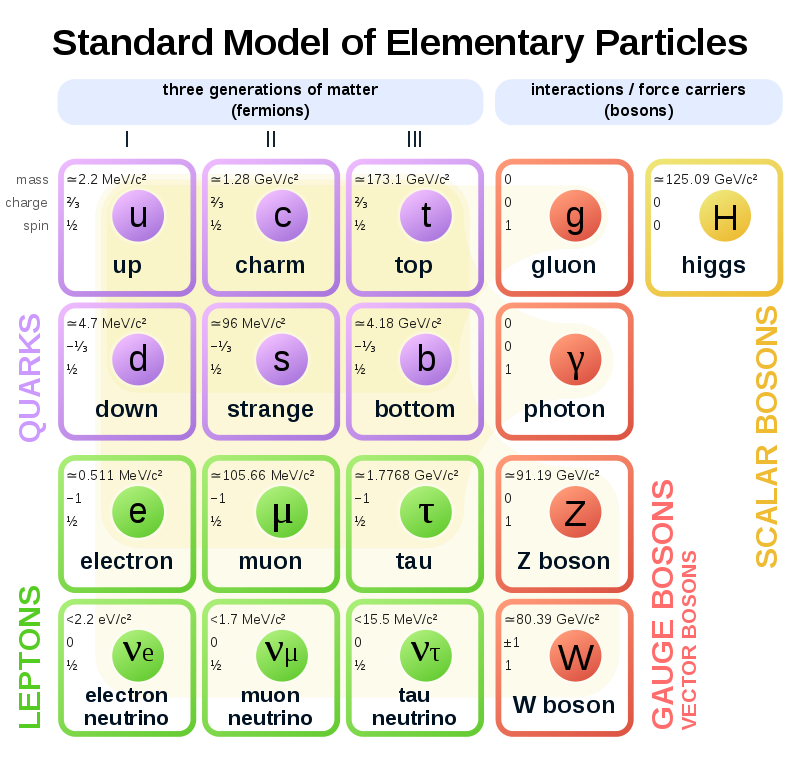
\includegraphics[width=.95\linewidth]{figs/chapter_intro/standard_model.png}
\caption{Standard model of fundamental particles. Each of the first three columns forms a generation of matter. The figure is taken from Ref.~\cite{wiki:standard_model}.}
\label{fig:intro_standard_model}
\end{figure}



\subsubsection{Color confinement}
\label{sec:color_confinement}

In QCD, color confinement is the phenomenon that color charged particles (quarks and gluons) cannot be isolated, and therefor cannot be directly observed under normal conditions. This means that quarks and gluons must clump together to form hadrons. The two main types of hadrons are the baryons (three quarks) and mesons (one quark, one antiquark). In addition, colorless glueball formed only of gluons are also consistent with color confinement, though difficult to identify experimentally.

The origin of color confinement lies within one feature of QCD: asymptotic freedom. Unlike QED, where the electric field interaction becomes stronger as the energy scale decreases, asymptotic freedom is a property of some gauge theories that causes interactions between particles to become asymptotically weaker as the energy scale increases and the corresponding length scale decreases. This phenomenon can be understood qualitatively by noting that the force-carrying gluons of QCD have color charge, unlike the photons of QED. Whereas the electric field between electrically charged particles decrease rapidly as those particles are separated, the gluon field between a pair of color charges forms a narrow flux (or string) between them. Because of this behavior of the gluon field, the strong force between the particles is constant regardless of their separation.

Therefore, as two quarks are separated, the energy increases, and at some point it becomes energetically favorable for a new quark-anti-quark pair to appear, rather than extending the string further. As a result of this, when quarks are produced in particle accelerators, instead of seeing the individual quarks in detectors, we observe jets of many color neutral particles clustered together. This process is called hadronization, fragmentation or string melting. As a conclusion, free strongly-interaction quarks can not be produced under normal conditions.



\subsubsection{QCD phase diagram}

Due to color confinement, no ``free'' quarks can be found in the hadronic matter. However, with finite spatial extension, concept of hadronic matter appears to lose its meaning at sufficiently high density. At low density, particular quark in a hadron ``knows'' its partner quark. However, at high density, when hadrons start to interpenetrate each other, a particular quark will not be able to identify the quark which was its partner at lower density~\cite{Chaudhuri:2012yt}. Effectively, once we have a system of mutually interpenetrating hadrons, where each quark finds a number of quarks in its vicinity, quarks behave just like they are ``free''. Similar phenomena can happen at high temperature. As the temperature of a nuclear matter is increased, more and more low mass hadrons will be created. The system again will be dense enough and hadrons will start to interpenetrate. It is customary to call this quark matter as QGP, which is a thermalized state of quarks and gluons, where quarks and gluons are free to move in a nuclear volume rather than a nucleonic volume. Even though the explanation above is over-simplified and on the conceptual level, it still illustrates an idea why QGP only exists in high density and temperature environment.

The phase diagram of quark matter is not well known, either experimentally or theoretically. A commonly conjectured form of phase diagram is shown in the Figure~\ref{fig:intro_QCD_diagram}, as a function of temperature $T$ and baryon chemical potential $\mu_B$. The solid line represents a first order transition which separates hadronic and QGP phase. The end point of this line is the Critical End Point (CEP). The dashed line at small $\mu_B$ indicates a cross-over transition between the QGP and hadronic phases.

\begin{figure}[H]
\centering
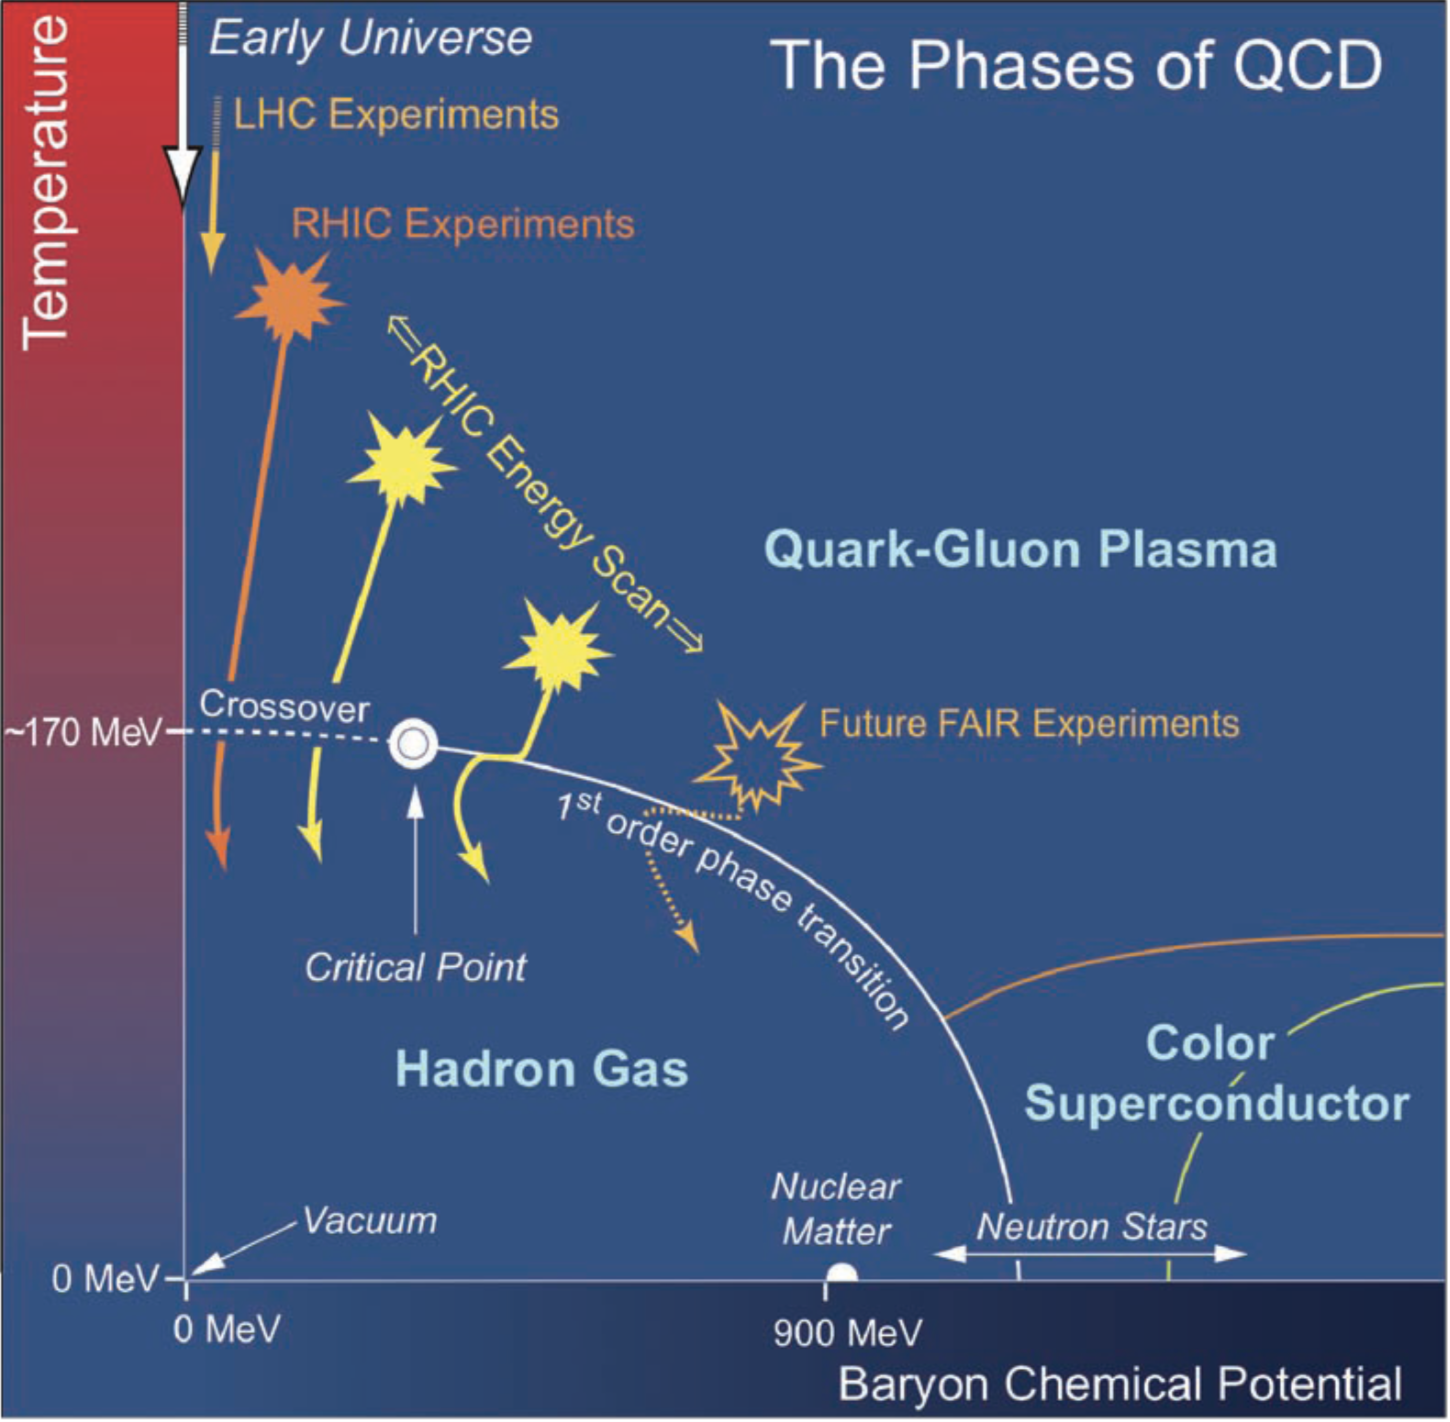
\includegraphics[width=.6\linewidth]{figs/chapter_intro/QCD_diagram.png}
\caption{Schematic QCD phase diagram for nuclear matter. The solid lines show the phase boundaries for the indicated phases. The solid circle depicts the critical point. Possible trajectories for systems created in the QGP phase at different accelerator facilities are also shown.}
\label{fig:intro_QCD_diagram}
\end{figure}

Theoretically, there are several approaches to locate the QCD phase transition boundary. Lattice QCD~\cite{Gupta:1997nd} (LQCD) is a well-established non-perturbative approach formulated on a grid or lattice of points in space and time. LQCD is favored because analytic or pertubative solutions in low-energy QCD are hard or impossible to obtain due to the high non-linear nature of the strong force and the large coupling constant at low energies. However, numerical LQCD calculations can be extremely computationally intensive, and currently there is no formulation of LQCD that allows us to simulate real-time dynamics of QGP. Another independent approach is to incorporate the QCD Lagrangian into MC models such as PYTHIA and HIJING. The results from these models provide important references for comparisons between models and experiments. We will follow this second approach in this dissertation.



\subsubsection{QGP in cosmology}

Why is QGP important to study? For a complete review, refer to Ref.~\cite{Busza:2018rrf}. In the early universe, when dense and temperature are very high, QGP is presumed to be existed. The timeline of big bang can be described as follows:
\begin{itemize}
\item At the earliest time, temperature is at the order of Planck scale temperature. At this stage, quantum gravity is important. String theorists are putting enormous efforts trying to understand this stage.
\item At the later stage of evolution, it is the grand unification scale. Strong and electroweak interactions are unified at this sale. The universe at this scale may also be supersymmetric, where each fermion a boson exists and vice-versa.
\item As the universe further expands and cools, strong and electroweak interactions are separated. At this lower temperature (100 GeV), electroweak symmetry breaks and Baryon asymmetry may be produced. Universe exists as QGP.
\item As temperature approaches 100 MeV, deconfinement-confinement transition occur, and hadrons are formed. All heavy-ion collisions are designed to study matter around this temperature.
\item At temperature 1 MeV, nucleosynthesis starts and light elements are formed. This temperature range is also well studied in nuclear physics experiments.
\item At temperature 1 eV, universe changes from ionised gas to a gas of neutral atoms and structures begin to form.
\end{itemize}

QGP may also exist at the core of a neutron star. Since the radius of neutron star is $\sim 10$ km, but very dense (10 times normal nuclear matter density), at such high density matter is likely to be in the form of QGP. The major difference between QGP at the early universe and that in neutron star is the temperature: at the core of the neutron star it is cold QGP with $T\sim 0$ MeV.



\subsubsection{QGP in heavy ion collision}
\label{sec:qgp_in_lab}

To achieve the high density and temperature for the generation of QGP in lab, over the past 15 years, scientists have been conducting Heavy Ion (HI) experiments by colliding nucleus with high energy. The evolution of HI collisions partially follows several stages of the early universe, and is illustrated in Figure~\ref{fig:intro_QGP_evolution}. In experiments, it is important to understand the evolution of HI collisions since we do not have direct access to the QGP itself. By measuring final stage particles and modeling initial conditions provide important constraints to the properties of QGP.

\begin{figure}[H]
\centering
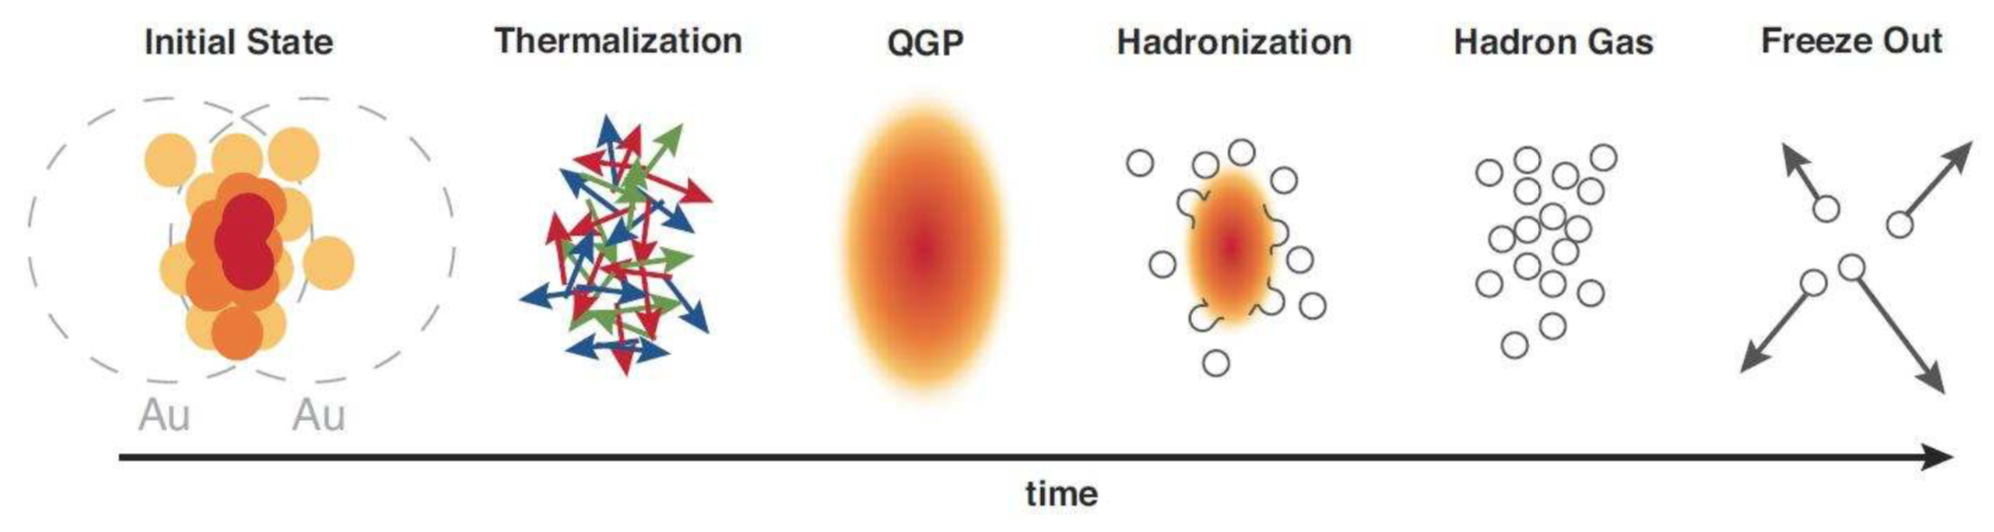
\includegraphics[width=.95\linewidth]{figs/chapter_intro/QGP_evolution.png}
\caption{Schematic illustration of the evolution of nuclear matter created in HI collision. The figure is taken from M. McCumber's PhD thesis.}
\label{fig:intro_QGP_evolution}
\end{figure}

Each stage in the HI collision is briefly discussed as follows:
\begin{itemize}
\item Initial state: in relativistic HI collisions, due to Lorentz contraction, nucleus appear to be "pancake" shape in the lab frame. Participating nucleons collide, generate entropy and produce a nuclear matter with non-uniform energy density. Such non-uniform geometry shape is an important feature for flow measurement, and can be described in two prevailing models: Glauber~\cite{Glauber:1955qq} and Color Glass Condensate (CGC)~\cite{Kharzeev:2002ei}. We will discuss Glauber model in details in Section~\ref{sec:glauber_model}.
\item Thermalization: participating quarks and gluons interact among each other and the system approaches thermal equilibrium. The thermalization time is approximately $\leq 1$ fm/c, a very rapid thermalization as suggested by hydrodynamic calculations~\cite{Adare:2009qk}.
\item QGP: the dense and equilibrated QGP is formed, which then continues to expand and cool down.
\item Hadronization: as the QGP expands, the energy density and temperature decrease, partons begin to form into bound state, i.e. hadrons. This process is named as "recombination" or "coalescence"~\cite{Fries:2008hs}. As discussed above, fragmentation is another different mechanism for partons to hadronize.
\item Hadron gas: at this stage, newly produced hadrons are weakly coupled and still exhibit collective behavior and the whole system is still in equilibrium. The system resembles a dilute gas and can be described by the transport models. Studies showed that the lifetime of this stage is so small that its influence is very limited~\cite{Afanasiev:2007tv}.
\item Freeze out: as the system keeps expanding and diluting, local thermal equilibrium breaks and interactions among hadrons are negligible. Finally the particles stop interact and are observed by the detectors.
\end{itemize}

HI physicists developed different observables that are sensitive to different stages of the HI evolutions, which are summarized in Section~\ref{sec:probing_qgp}, after we introduce the kinematics in HI collision.



\subsection{Kinematics of HI collisions}

To make this dissertation self-consistent, we will introduce kinematics of HI collisions~\cite{Chaudhuri:2012yt}. In relativistic nucleus-nucleus collisions, since the nucleus in the initial stage and particles particles from the final stage travel at the speed close to light, it is convenient to use kinematic variables which take simple form under Lorentz transformation, after changing the frame of reference. In this section, we will first briefly introduce the Lorentz transformation, then discuss several key kinematics frequently used in HI collisions.



\subsubsection{Lorentz transformation}

If $x^\mu$ is the coordinate in one frame of reference, then in another frame of reference the coordinates $x'^{\mu}$ must satisfy:
\begin{equation}
g_{\mu\nu} dx'^\mu dx'^\nu = g_{\mu\nu} dx^\mu dx^\nu
\end{equation}
where Einstein's summation convention is used. $g_{\mu\nu}$ is called the space-time metric:
\begin{equation}
g_{\mu\nu} \equiv diag(1, -1, -1, -1),
\end{equation}
and the natural units $c=1$ is assumed:

In other words, the Lorentz transformation keeps the space-time distance invariant under the transformation. It also has one special property that the speed of light is same in the two frame of reference.

A general Lorentz transformation consists of rotation and translation. Lorentz transformation without rotation is called Lorentz boost. For example, consider the Lorentz boost along the $z$ direction by velocity $\beta$. The transformation can then be written as:
\begin{equation}
\begin{bmatrix}
t' \\
z'
\end{bmatrix}
=
\begin{bmatrix}
\gamma & -\beta\gamma \\
-\beta\gamma & \gamma
\end{bmatrix}
\begin{bmatrix}
t \\
z
\end{bmatrix}
\end{equation}
where $\gamma = 1/\sqrt{1-\beta^2}$ is the Lorentz factor.



\subsubsection{Rapidity variable}

In relativistic energy, rapidity is defined as:
\begin{equation}
\begin{split}
y &= \frac{1}{2} \ln \frac{E+p_z}{E-p_z} \\
&= \tanh^{-1}(\beta_L)
\end{split}
\end{equation}
where $\beta_L = p_z / E$ is called the longitudinal velocity. Rapidity has the advantage over $\beta_L$ that they are additive under a longitudinal boost: a particle with rapidity $y$ in a give frame has rapidity $y + dy$ in a frame which moves relative to the first frame with rapidity $dy$ in the $-z$ direction. This is because the relativistic velocity $\beta_1$ and $\beta_2$ fulfill the addition formula:
\begin{equation}
\beta = \frac{\beta_1 + \beta_2}{1 + \beta_1 \beta_2},
\end{equation}
which is exactly the addition formula for hyperbolic tangents:
\begin{equation}
\tanh (y_1 + y_2) = \frac{\tanh(y_1) + \tanh(y_2)}{1 + \tanh(y_1)\tanh(y_2)}.
\end{equation}

Rapidity is the relativistic analog of non-relativistic velocity. In the non-relativistic limit $p \ll m$, rapidity can be written as:
\begin{equation}
\begin{split}
y &= \frac{1}{2} \ln \frac{\sqrt{p^2 + m^2} + mv_z}{\sqrt{p^2 + m^2} - mv_z} \\
&= \frac{1}{2} [\ln(1+v_z) - \ln(1-v_z)] \\
&\approx v_z
\end{split}
\end{equation}

In terms of the rapidity variables, particle 4-momentum can be parameterized as:
\begin{equation}
p^\mu = (E, p_x, p_y, p_z) = (m_T \cosh y, p_x, p_y, m_T \sinh y)
\end{equation}
with transverse mass $m_T \equiv \sqrt{m^2 + \pT^2} = \sqrt{m^2 + p_x^2 + p_y^2}$.



\subsubsection{Pseudorapidity variable}

For a particle emitted at an angle $\theta$ with respect to the beam axis, rapidity variable can be written as:
\begin{equation}
\begin{split}
y &= \frac{1}{2} \ln \frac{E + p_z}{E - p_z} \\
&= \frac{1}{2} \ln \frac{\sqrt{m^2 + p^2} + p\cos\theta}{\sqrt{m^2 + p^2} - p\cos\theta}
\end{split}
\end{equation}

At very high energy, we have $p \gg m$, and the mass term can be neglected:
\begin{equation}
\begin{split}
y &= \frac{1}{2} \frac{p + p\cos\theta}{p - p\cos\theta} \\
&= - \ln \frac{\theta}{2} \\
&\equiv \eta,
\end{split}
\end{equation}
where $\eta$ is called pseudorapidity. Only angle $\theta$ determine the pseudorapidity. It is a very convenient parameter for experimentalists since details of particles, like mass and full momentum, are not known. While angle of emission $\theta$ can be easily measured experimentally.



\subsubsection{Invariant distribution}

In experiment, one key observable is the distribution of final stage particles. We will construct a Lorentz boost invariant observable that is related to particle distribution.

The differential of Lorentz boost in longitudinal direction is:
\begin{equation}
\begin{split}
dp'_z &= \gamma (dp_z - \beta E) = \gamma (dp_z - \beta \frac{p_z dp_z}{E}) \\
&= \frac{dp_z}{E}\gamma(E - \beta p_z) = \frac{dp_z}{E} E',
\end{split}
\end{equation}
where $EdE = p_z dp_z$ has been used. This means $dp_z / E$ is Lorentz invariant. Since $\pT$ is also Lorentz invariant, $d^3p / E$ is Lorentz invariant.

Then we can construct the Lorentz invariant differential yield:
\begin{equation}
E\frac{d^3 N}{d^3 p} = E\frac{d^3 N}{d^2 \pT dp_z} = \frac{d^3 N}{d^2 \pT dy},
\end{equation}
where the relation $dp_z / E = dy$ is used. Some times experimental results are given in terms of pseudorapidity. The transformation from $(y, \pT)$ to $(\eta, \pT)$ is written as follows:
\begin{equation}
\frac{d^3 N}{d\eta d\pT} = \sqrt{1 - \frac{m^2}{m^2_T \cosh^2 y}}\frac{d^3 N}{dy d\pT}
\end{equation}



\subsubsection{Luminosity}

The luminosity is an important parameter in collider experiments. The reaction rate in a collider is given by:
\begin{equation}
R = \sigma L,
\end{equation}
where $\sigma$ is the interaction cross section and $L$ is the luminosity, in the unit of $\text{cm}^{-2}\text{s}^{-1}$. The luminosity is defined as:
\begin{equation}
L = f n \frac{N_1 N_2}{A},
\end{equation}
where:
\begin{itemize}
\item $f$: revolution frequency
\item $N_1$: number of particles in bunch 1
\item $N_2$: number of particles in bunch 2
\item $n$: number of bunches in one beam in the storage ring
\item $A$: cross-sectional area of the beams
\end{itemize}



\subsubsection{Collision geometry}

In HI collisions, since the number of nucleons is large, nucleus can be approximated as a round shape, as shown in Figure~\ref{fig:intro_HI_geometry}. The impact parameter $b$ is defined as the distance between the centers of nucleus. Due to the elliptic shape of the overlapping region, different kinds of planes can be defined:
\begin{itemize}
\item Reaction Plane (RP): supported by the vector of impact parameter and the beam direction;
\item Participant Plane (PP): supported by the average vector of participants and the beam direction;
\item Event Plane (EP): supported by the average vector of final particles and the beam direction.
\end{itemize}
The reaction and participant planes are defined in the initial stage, thus cannot be measured in experiment directly. While the event plane is one of the key observables in flow analysis.

\begin{figure}[H]
\centering
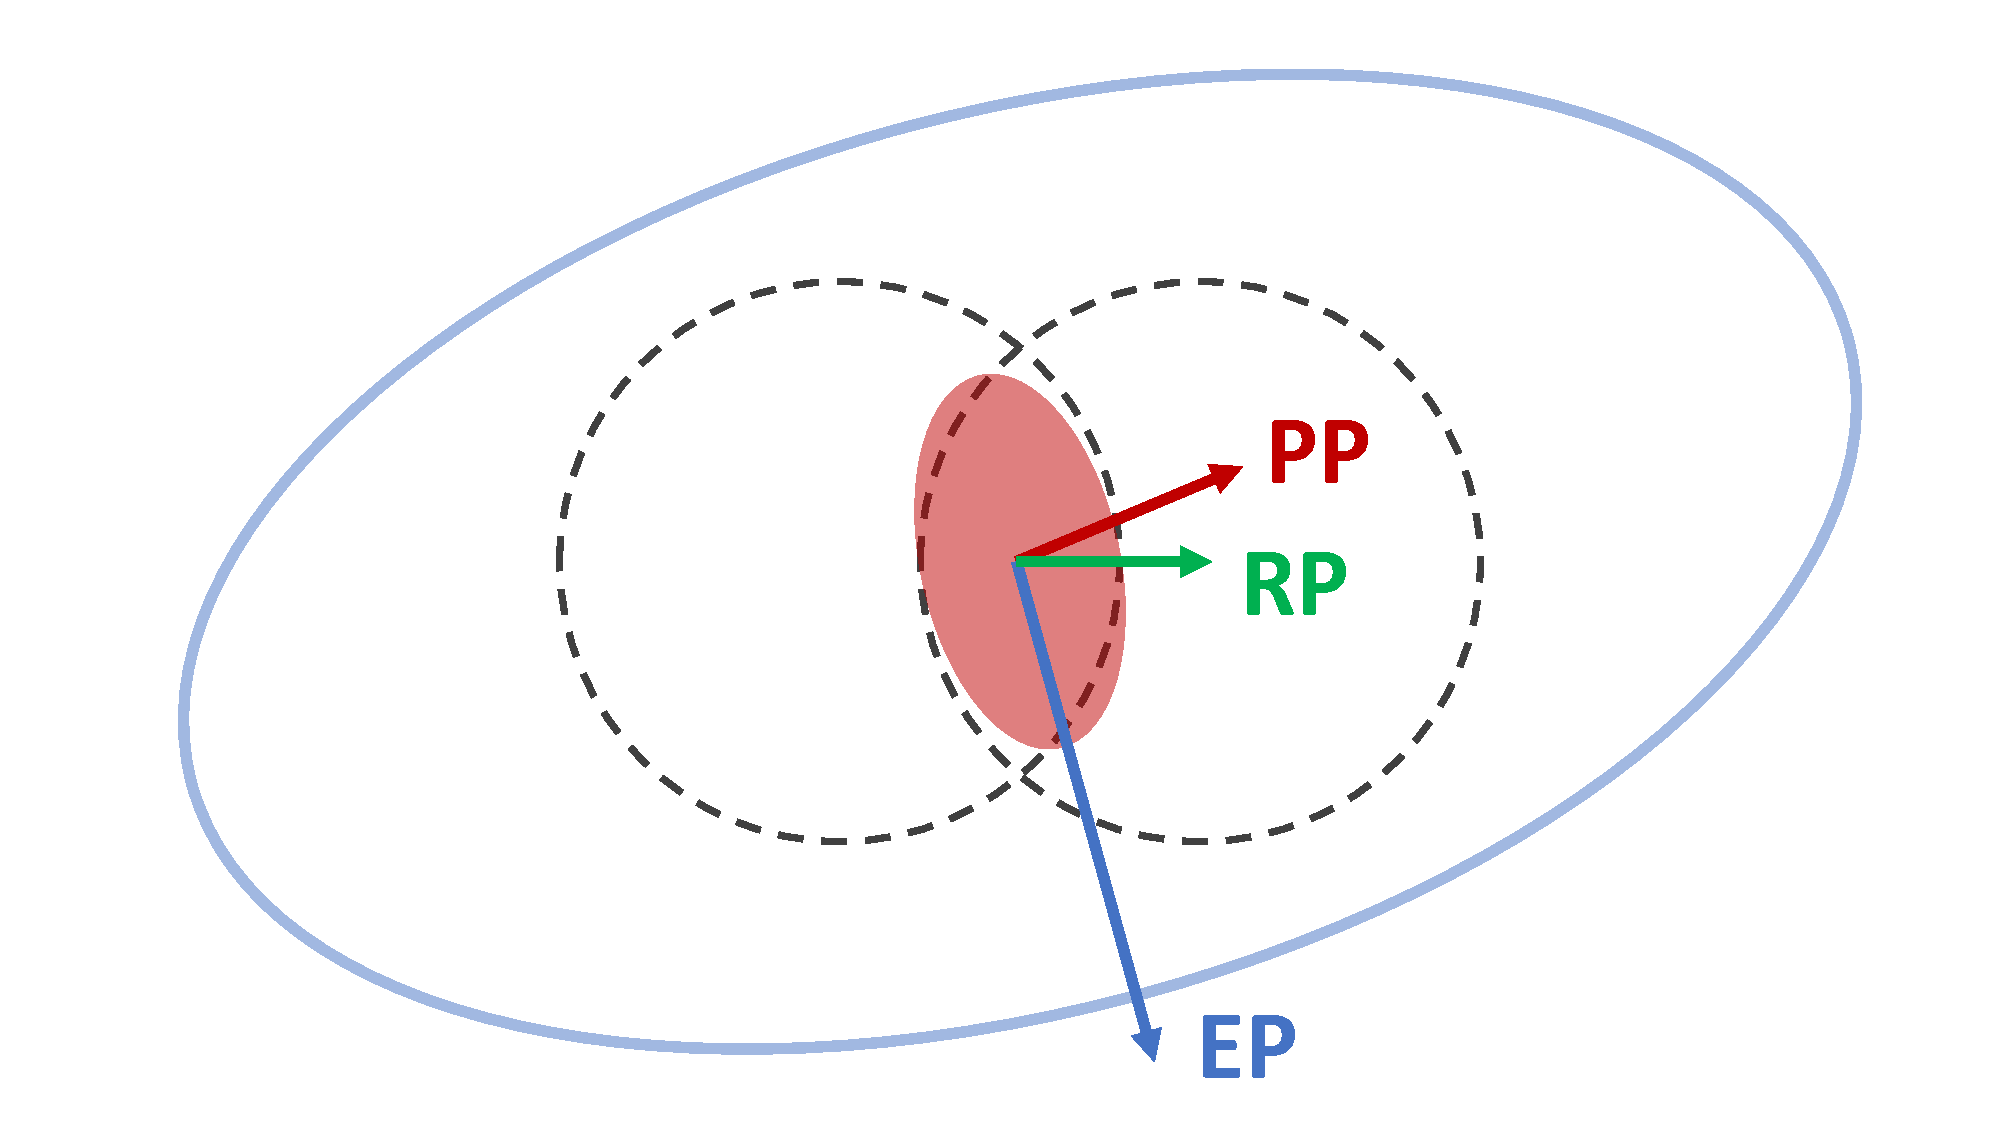
\includegraphics[width=.7\linewidth]{figs/chapter_intro/HI_geometry}
\caption{The definitions of the Reaction Plane (RP), Participant Plane (PP) and Event Plane (EP).}
\label{fig:intro_HI_geometry}
\end{figure}

The particle azimuthal distribution measured with respect to the event plane is not isotropic, and it is conventional to expand it in a Fourier series:
\begin{equation}
E \frac{d^3 N}{d^3 p} = \frac{1}{2\pi} \frac{d^2 N}{\pT d\pT dy}[1+\sum_{n=1} 2 v_n \cos (n(\phi-\Psi))]
\end{equation}
where $\Psi$ is the azimuthal angle of event plane. Note that the left part of the equation is boost invariant. The flow harmonics $v_n$ can be calculated as:
\begin{equation}
v_n = \lr{\cos (n(\phi - \Psi))}
\end{equation}
where the angle brackets mean an average over all particles in all events. Flow coefficients are used for a quantitative characterization of the event anisotropy. The sine term are not present because of the symmetric with respect to the reaction plane.



\subsubsection{Centrality}

Depending upon the impact parameter of the collision, several types of collisions can be defined:
\begin{itemize}
\item Central collision: two nuclei collide head on;
\item Peripheral collision: only glancing interaction between two nuclei.
\end{itemize}
One could image the system created in a central collision can be very different different from that created in a peripheral collision, thus it is crucial to study the observables as a function of impact parameter. Impact parameter of a collision can not be measured experimentally, however, one can have an one-to-one correspondence between impact parameter and some experimental observable. In practice, particle multiplicity $\Nch$ and transverse energy $\Et$ are used since they are monotonic functions of impact parameter. In other cases, by utilizing the detector very far away from the collision point, energy of the spectators can also be an anti-correlated proxy for the impact parameter. See Section~\ref{sec:zero_degree_calorimeter} for details.

The grouping of the events can be done quantitatively. Define a minimum bias collision where all possible collisions are allowed. Figure~\ref{fig:intro_HI_centrality} illustrates how centrality is defined. In this example, distribution of charged particle multiplicity $\Nch$ from $|\eta|<1$ in a minimum bias collision is cut into successive intervals starting from maximum value of multiplicity. First $5\%$ of the high $\Nch$ events corresponds to the top $5\%$ or $0-5\%$ collision centrality. Similarly, centrality class can be defined by measuring the transverse energy.

\begin{figure}[H]
\centering
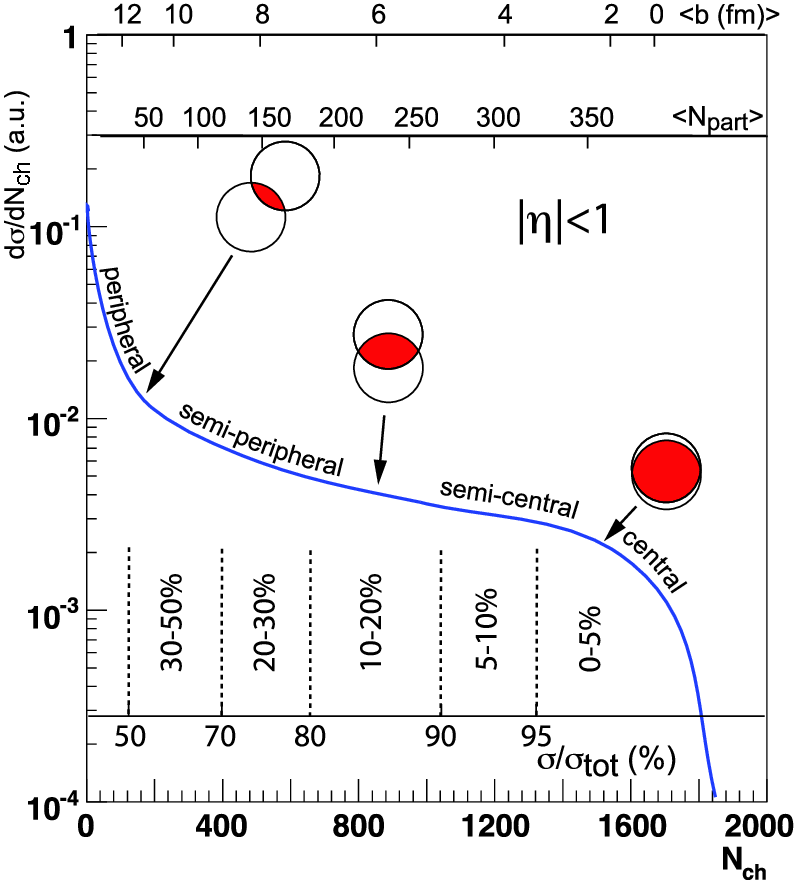
\includegraphics[width=.5\linewidth]{figs/chapter_intro/HI_centrality.png}
\caption{The correlation between the number of participating nucleons in a heavy-ion collision, their cross section and the impact parameter $b$, defining the centrality classes. This figure is taken from Ref.~\cite{Betz:2009jw}.}
\label{fig:intro_HI_centrality}
\end{figure}

Instead of impact parameter, one often defines centrality in terms of number of participating nucleons $N_\text{part}$ (as shown in Figure~\ref{fig:intro_HI_centrality}) or in terms of binary nucleon collision number. These measures have one-to-one relationship with impact parameter and can be calculated in any initial stage models, like Glauber model.



\subsection{Examples of QGP probes}
\label{sec:probing_qgp}

As discussed in Section~\ref{sec:qgp_in_lab}, experimentally it is not possible to probe the QGP directly. In this section, we will present an overview of several major experimental observables that are used to probe the existence and properties of QGP.

\subsubsection{Strangeness production}

The study of the properties of QGP can be undertaken using quarks not present in daily matter observed around us. The experimental and theoretical work relies on the idea of strangeness enhancement. Unlike the up and down quarks, strange quarks are not brought into the reaction by the colliding nuclei. Therefore, any strange quarks or antiquarks observed in experiments have been made from the kinetic energy of colliding nuclei. Furthermore, the mass of strange quarks and antiquarks is equivalent to the temperature or energy at which protons, neutrons and other hadrons dissolve into quarks. This means that the abundance of strange quarks is sensitive to the conditions, structure and dynamics of the deconfined matter phase, and if their number is large it can be assumed that deconfinement conditions were reached.

Strange quarks are naturally radioactive and decay by weak interactions into lighter quarks on a timescale that is extremely long compared with the nuclear-collision time. This makes it relatively easy to detect strange particles through the tracks left by their decay products. Measurement of abundant formation of $K_S^0$, $\Lambda$, $\Xi$ and $\Omega$ as well as their antiparticles is an important observation claiming that QGP has been formed. This abundant formation is often presented in comparison with the scaled expectation from normal proton-proton collisions.

In Figure~\ref{fig:intro_strangeness_ALICE}, the ratios of the yields of $K_S^0$, $\Lambda$, $\Xi$ and $\Omega$ to the pion $(\pi^+ + \pi^-)$ yield as a function of $\lr{d\Nch / d\eta}$ are compared to $p$+Pb and Pb+Pb results at the LHC~\cite{ALICE:2017jyt}. A significant enhancement of strange to non-strange hadron production is observed with increasing particle multiplicity in $pp$ collision. The behavior observed in $pp$ collisions resembles that of $p$+Pb collisions at a slightly lower center-of-mass energy, in terms of both the values of the ratios and their evolution with multiplicity. At high multiplicity, the yield ratios reach values similar to the ones observed in Pb+Pb collisions, where no significant change with multiplicity is observed beyond an initial slight rises. For a more complete review on strangeness enhancement, refer to Ref.~\cite{Koch:2017pda}.

\begin{figure}[H]
\centering
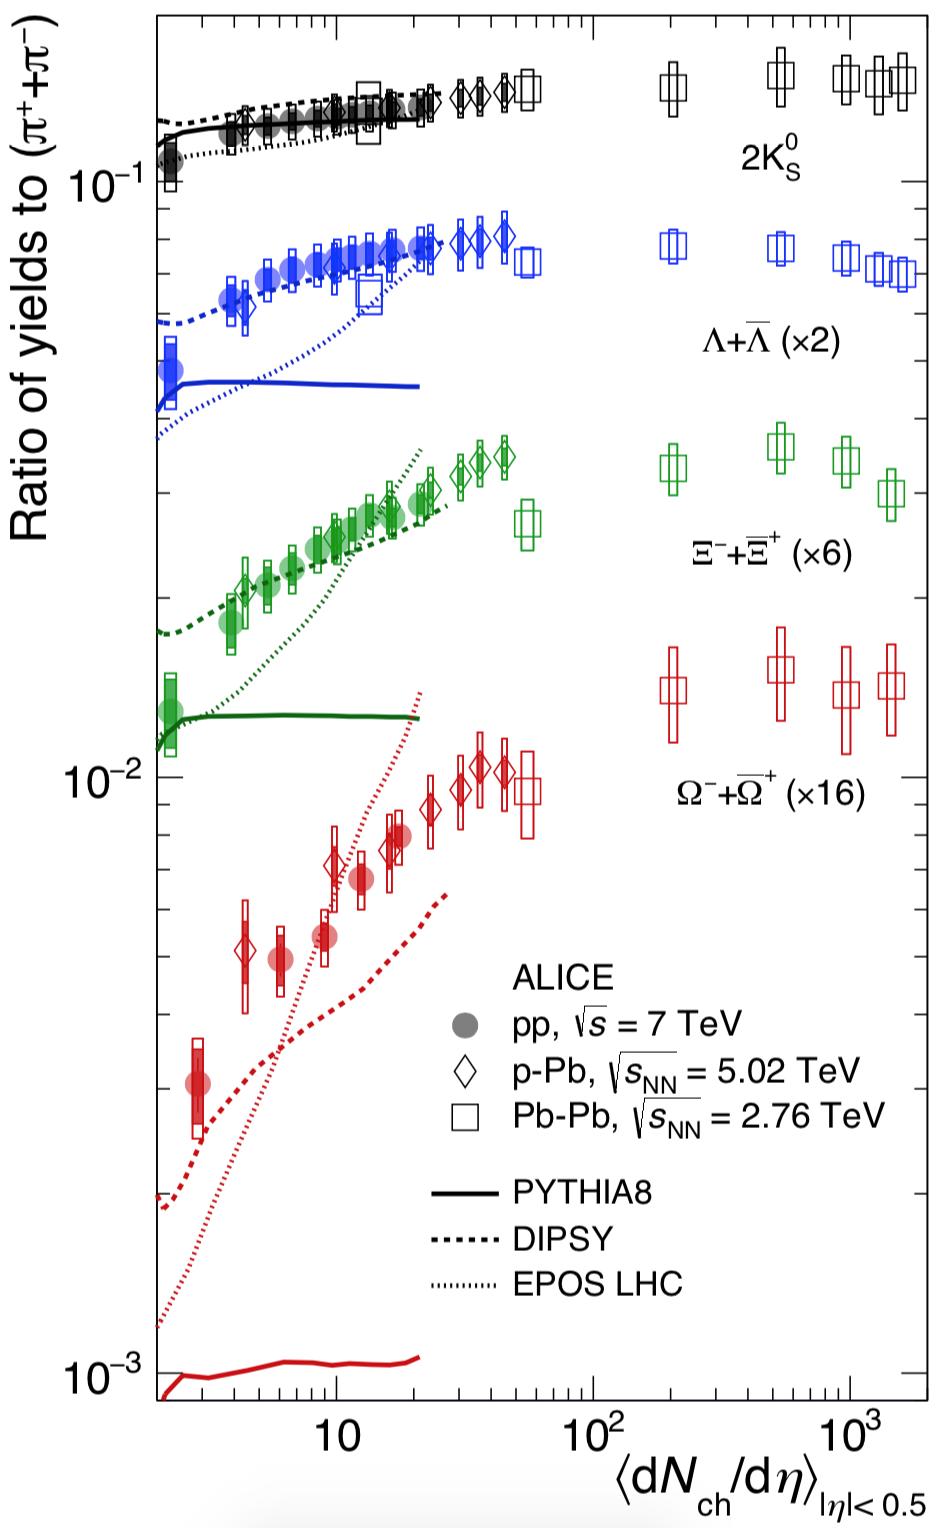
\includegraphics[width=.5\linewidth]{figs/chapter_intro/strangeness_ALICE.png}
\caption{$\pT$ integrated yield ratios to pions as a function of $\lr{d\Nch / d\eta}$ measured in $|y|<0.5$. The values are compared to calculations from MC models and to results obtained in $p$+Pb and Pb+Pb collisions at the LHC. This figure is taken from Ref.~\cite{ALICE:2017jyt}.}
\label{fig:intro_strangeness_ALICE}
\end{figure}



\subsubsection{Elliptic flow}

Elliptic flow describes the azimuthal momentum space anisotropy of particle emission from non-central HI collisions in the plane transverse to the beam direction, and is defined as the second harmonic coefficient of the azimuthal Fourier decomposition of the momentum distribution. Elliptic flow is a fundamental observable since it directly reflects the initial spatial anisotropy, of the nuclear overlap region in the transverse plane, directly translated into the observed momentum distribution of identified particles. Since the spatial anisotropy is largest at the beginning of the evolution, elliptic flow is especially sensitive to the early stages of system evolution. With absence of QGP, distribution of free-streaming particle will be uniform in the transverse direction, thus elliptic flow is strong evidence for the existence of QGP. The focus of this dissertation will be on elliptic flow and we will extend the discussions in Section~\ref{sec:transverse_measurements}.

Figure~\ref{fig:intro_v2_ALICE} presents the comparison of the fully $\pT$ integrated $v_2$ measured in the $20-30\%$ centrality in Pb+Pb collisions with results at lower energies~\cite{Adam:2016izf}. A continuous increase of anisotropic flow for this centrality has been observed from SPS/RHIC to LHC energies. For these fully $\pT$ integrated coefficients, an increase of $5\%$ is observed going from $\sqrt{s_\text{NN}}=2.76$ to 5.02 TeV, which is close to values of the hydrodynamic calculations. For a complete review on collective flow and hydrodynamics, refer to Ref.~\cite{Heinz:2013th, Jeon:2015dfa}.

\begin{figure}[H]
\centering
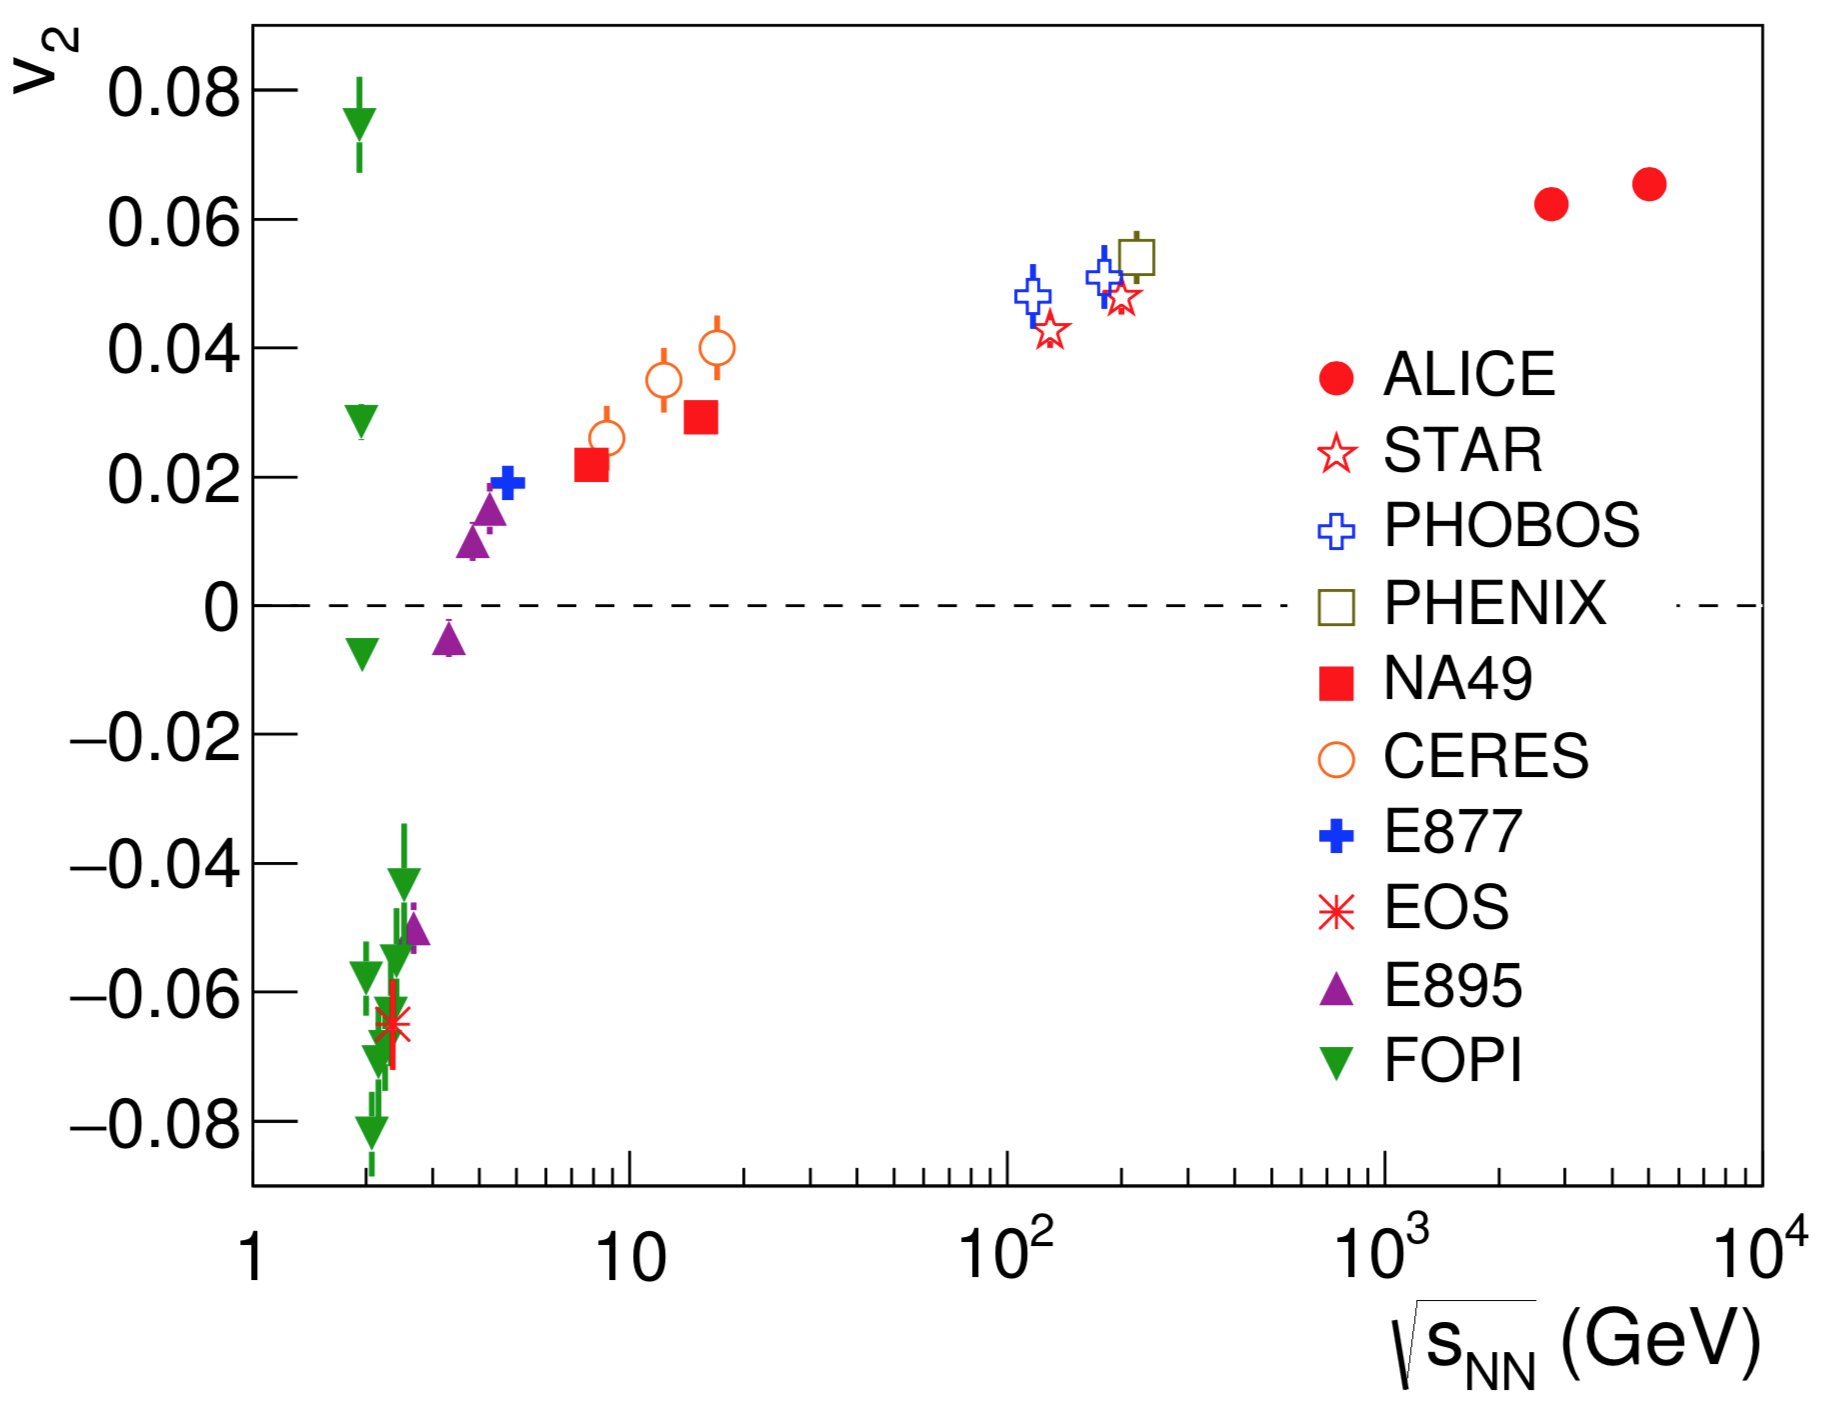
\includegraphics[width=.6\linewidth]{figs/chapter_intro/v2_ALICE.png}
\caption{Integrated elliptic flow $v_2\{4\}$ for the $20-30\%$ most central Pb+Pb collisions at $\sqrt{s_\text{NN}}=5.02$ TeV compared with $v_2$ measurements at lower energies with similar centralities. This figure is taken from Ref.~\cite{Adam:2016izf}.}
\label{fig:intro_v2_ALICE}
\end{figure}



\subsubsection{Jet quenching}

QCD jet produced from early stage collisions of beam quarks and gluons from two nuclei play an essential role in studying transport properties of the QGP produced in these energetic collisions~\cite{Qin:2015srf}. During their propagation through the hot and dense medium, the interaction between hard jets and the colored medium will lead to parton energy loss, denoted as jet quenching. During the last decades, there have been many striking experimental signatures of jet energy loss at RHIC and LHC. 

Figure~\ref{fig:intro_jet_RAA_ATLAS} shows the measurements of the nuclear modification factor $R_{AA}$ for inclusive jet production in Pb+Pb collisions~\cite{Aaboud:2018twu}. The inclusive jet nuclear modification factor $R_{AA}$ is defined as follows:
\begin{equation}
R_{AA}^\text{jet} = \frac{\frac{1}{N_\text{evt}}\frac{d^2 N_\text{jet}}{d\pT dy}|_\text{cent}}{\lr{T_{AA}}\frac{d^2 \sigma_\text{jet}}{d\pT dy}|_{pp}},
\end{equation}
where $N_\text{jet}$ and $\sigma_\text{jet}$ are the jet yield in Pb+Pb collisions and the jet cross-section in $pp$ collisions, respectively. $N_\text{evt}$ is the total number of Pb+Pb collisions within a chosen centrality interval. A clear suppression of jet production in central Pb+Pb collisions relative to $pp$ collision is observed. In the $0-10\%$ centrality interval, $R_{AA}$ is approximately 0.45 at $\pT=100$ GeV, and is observed to grow slowly (quenching decreases) with increasing jet $\pT$, reaching a value of 0.6 for jets with $\pT$ around 800 GeV.
\begin{figure}[H]
\centering
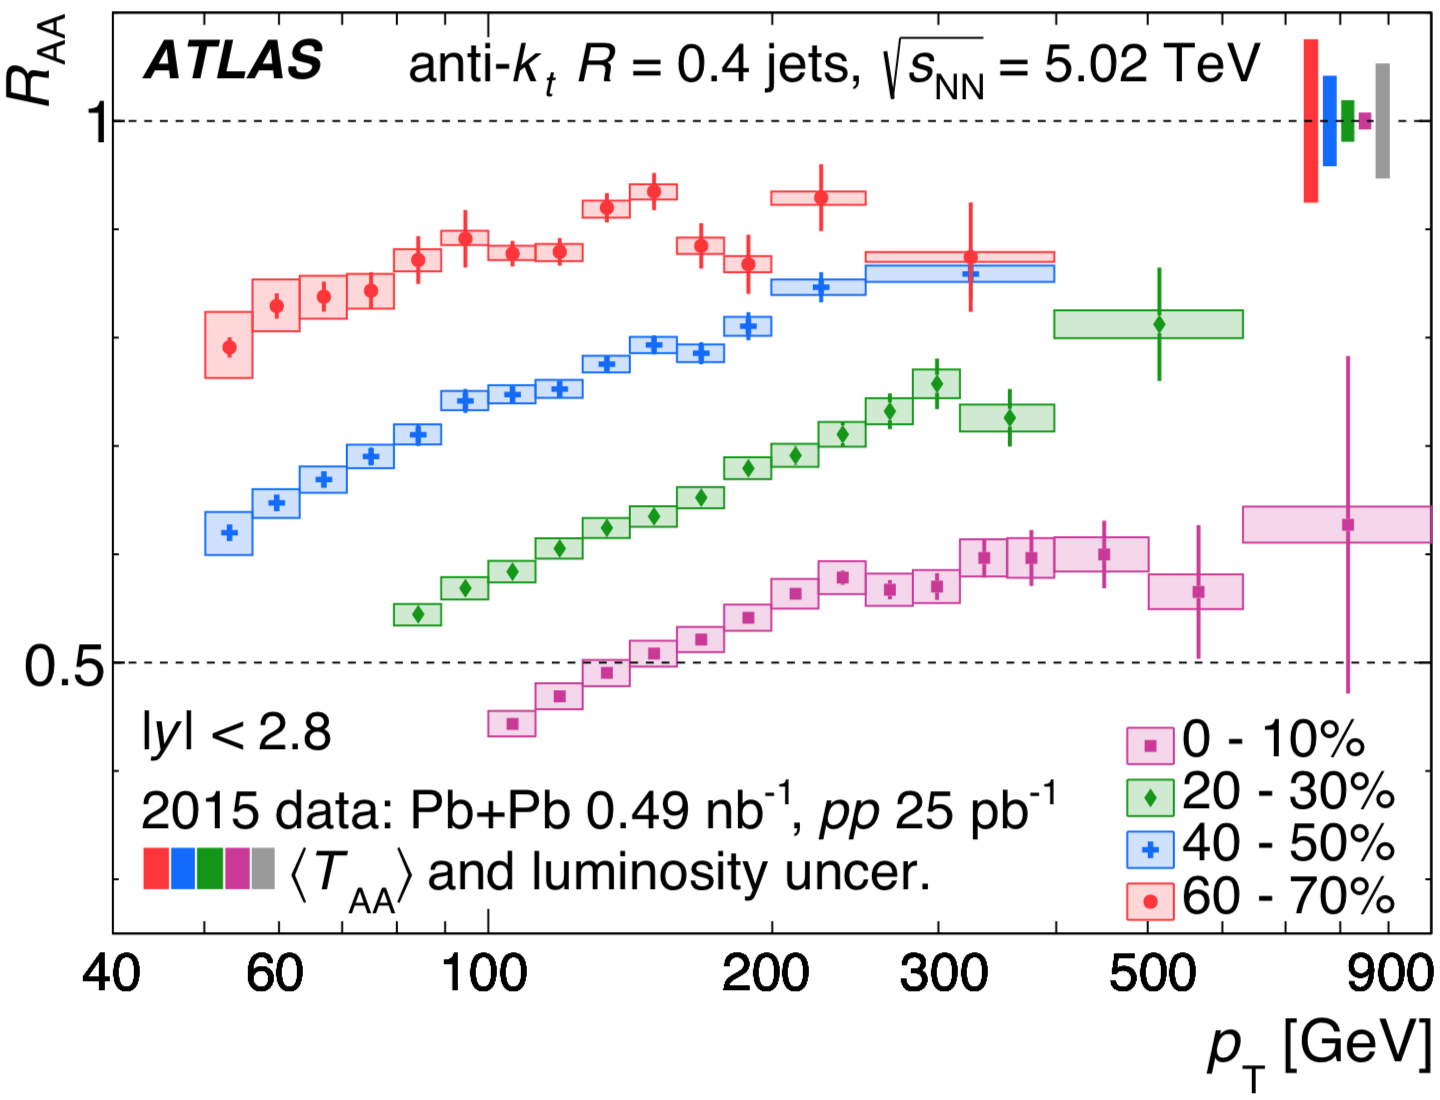
\includegraphics[width=.6\linewidth]{figs/chapter_intro/jet_RAA_ATLAS.png}
\caption{The $R_{AA}$ values as a function of jet $\pT$ for jets with $|y|<2.8$ for four centrality intervals. This figure is taken from Ref.~\cite{Aaboud:2018twu}.}
\label{fig:intro_jet_RAA_ATLAS}
\end{figure}

Another approach to study the effect of jet-medium interaction is the correlated back-to-back jet pairs~\cite{Qin:2015srf}. The energy loss of full jets can be studied by measuring the imbalance/asymmetry of the transverse energies between two correlated jets. The energy asymmetry factor $A_J$ for the correlated jet pairs is defined as:
\begin{equation}
A_J = \frac{E_{\text{T},1}-E_{\text{T},2}}{E_{\text{T},1}+E_{\text{T},2}},
\end{equation}
where $E_{\text{T}, i}$ denotes the transverse energy of the leading and sub-leading jets, respectively. The relative azimuthal angle $\Delta\phi \equiv |\phi_1 - \phi_2|$ between two correlated jets can also provide information about the degree of deflection that jet experience after passing through the hot and dense QGP medium.

The dijet asymmetry and $\Delta\phi$ distributions are shown in four centrality bins in Figure~\ref{fig:intro_jet_asym_ATLAS}, where they are compared with proton-proton data and with fully reconstructed HIJING + PYTHIA simulated events~\cite{Aad:2010bu}. The dijet asymmetry in peripheral Pb+Pb events is similar to that in both $pp$ and simulated events; however, as the events become more central, the Pb+Pb data distributions develop different characteristics, indicating an increased rate of highly asymmetric dijet events. The $\Delta\phi$ distributions show that the leading and second jets are primarily back-to-back in all centrality bins; however, a systematic increase is observed in the rate of second jets at large angles relative to the recoil direction as the events become more central. For a more complete review on jet quenching, refer to Ref.~\cite{dEnterria:2009xfs}.
\begin{figure}[H]
\centering
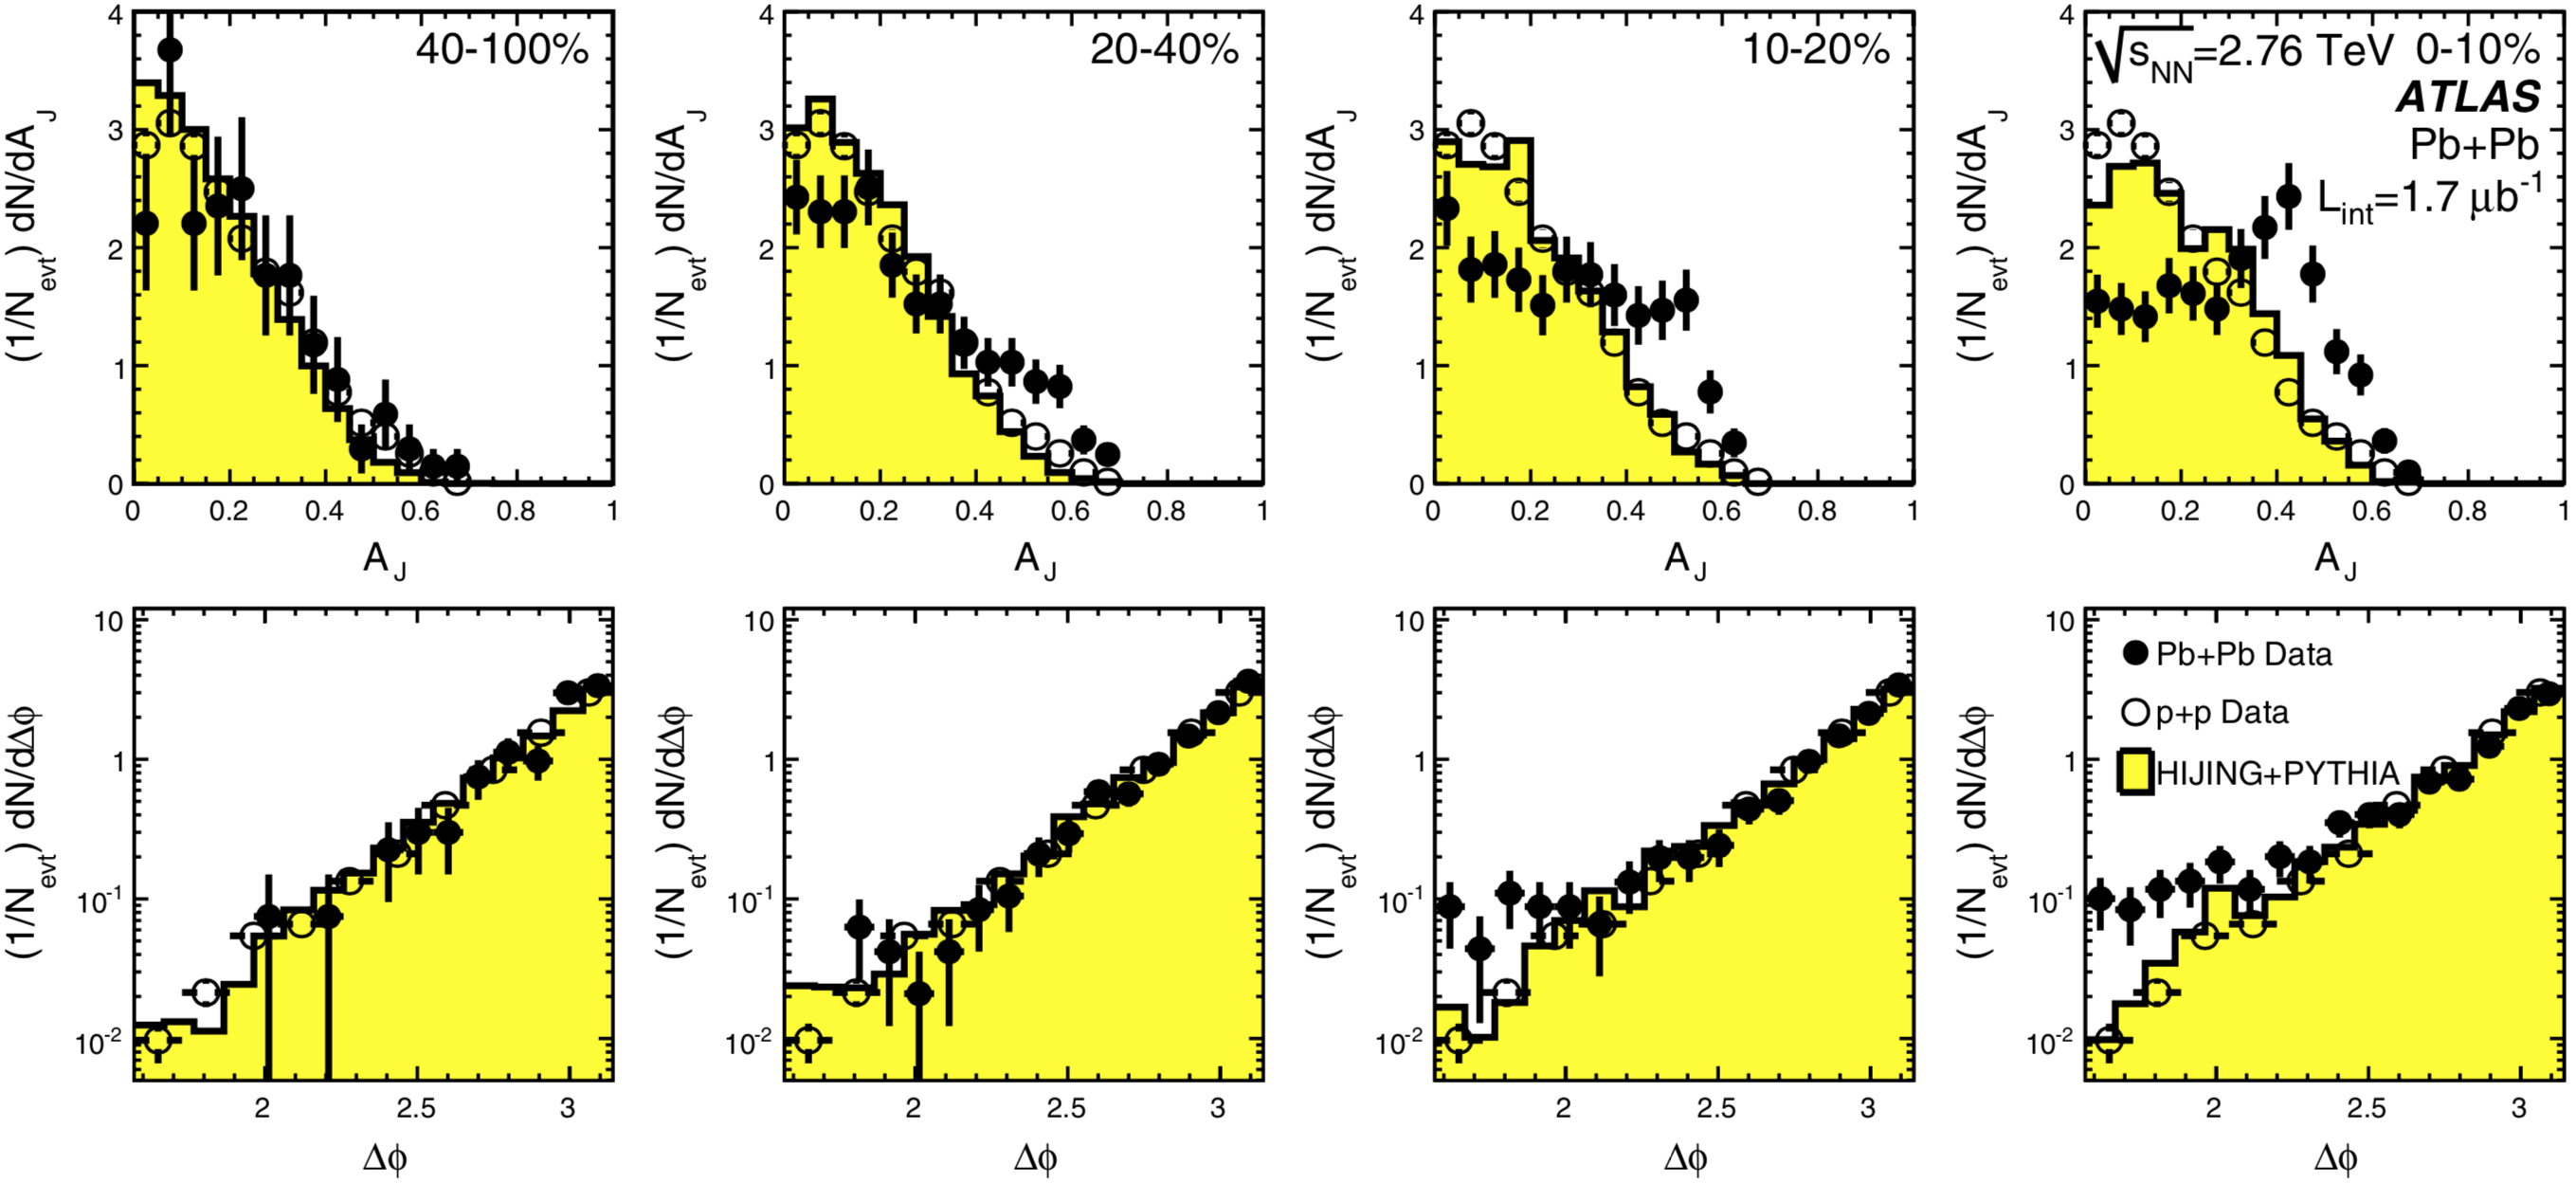
\includegraphics[width=.95\linewidth]{figs/chapter_intro/jet_asym_ATLAS.png}
\caption{Top: dijet asymmetry distribution for data and unquenched HIJING with superimposed PYTHIA dijets, as a function of centrality. Proton-proton data, analyzed with the same jet selection, are shown as open circles. Bottom: Distribution of $\Delta\phi$, the azimuthal angle between the two jets, for data and HIJING + PYTHIA, also as a function of centrality. This figure is taken from Ref.~\cite{Aad:2010bu}.}
\label{fig:intro_jet_asym_ATLAS}
\end{figure}



\subsubsection{Fluctuations of conserved quantities}

Experimental confirmation of the existence of the critical point will be the most direct verification of QCD theory in the non-perturbative region and evidence of the existence of QGP~\cite{Luo:2015cea}. Fluctuations of conserved quantities, such as net-baryon, net-charge and net-strangeness, are predicted to be sensitive to the correlation length of the system~\cite{Stephanov:2008qz} and directly connected to the susceptibilities computed in the theoretical calculations~\cite{Gupta:2011wh}. Thus it can serve as a powerful tool to probe the phase transition and critical point signal in heavy-ion collisions.

Figure~\ref{fig:intro_CP_STAR} shows the energy dependence of $S\sigma$ (ratio of 3rd-order and 2nd-order cumulant) and $\kappa\sigma^2$ (ratio of 4th-order and 2nd-order cumulant) for $\Delta N_p \equiv N_p^+ - N_p^-$ for Au+Au collisions for two collision centralities~\cite{Adamczyk:2013dal}. The $S\sigma$ values normalized to the corresponding Skellam expectations are shown in the bottom panel. The Skellam expectations reflect a system of totally uncorrelated, statistically random particle production. The corresponding results from the $pp$ collisions are also shown and found to be similar to peripheral Au+Au collisions. The data also show deviations from the hadron resonance gas model. The deviations of $S\sigma$ and $\kappa\sigma^2$ below Skellam expectation are qualitatively consistent with a QCD based model which includes a critical point. However the UrQMD model which does not include a critical point also shows deviations from the Skellam expectations. Hence conclusions on the existence of critical point can be made only after multiple sources of backgrounds are removed. For a more complete review of fluctuations of conserved quantities, refer to Ref.~\cite{Luo:2017faz}.
\begin{figure}[H]
\centering
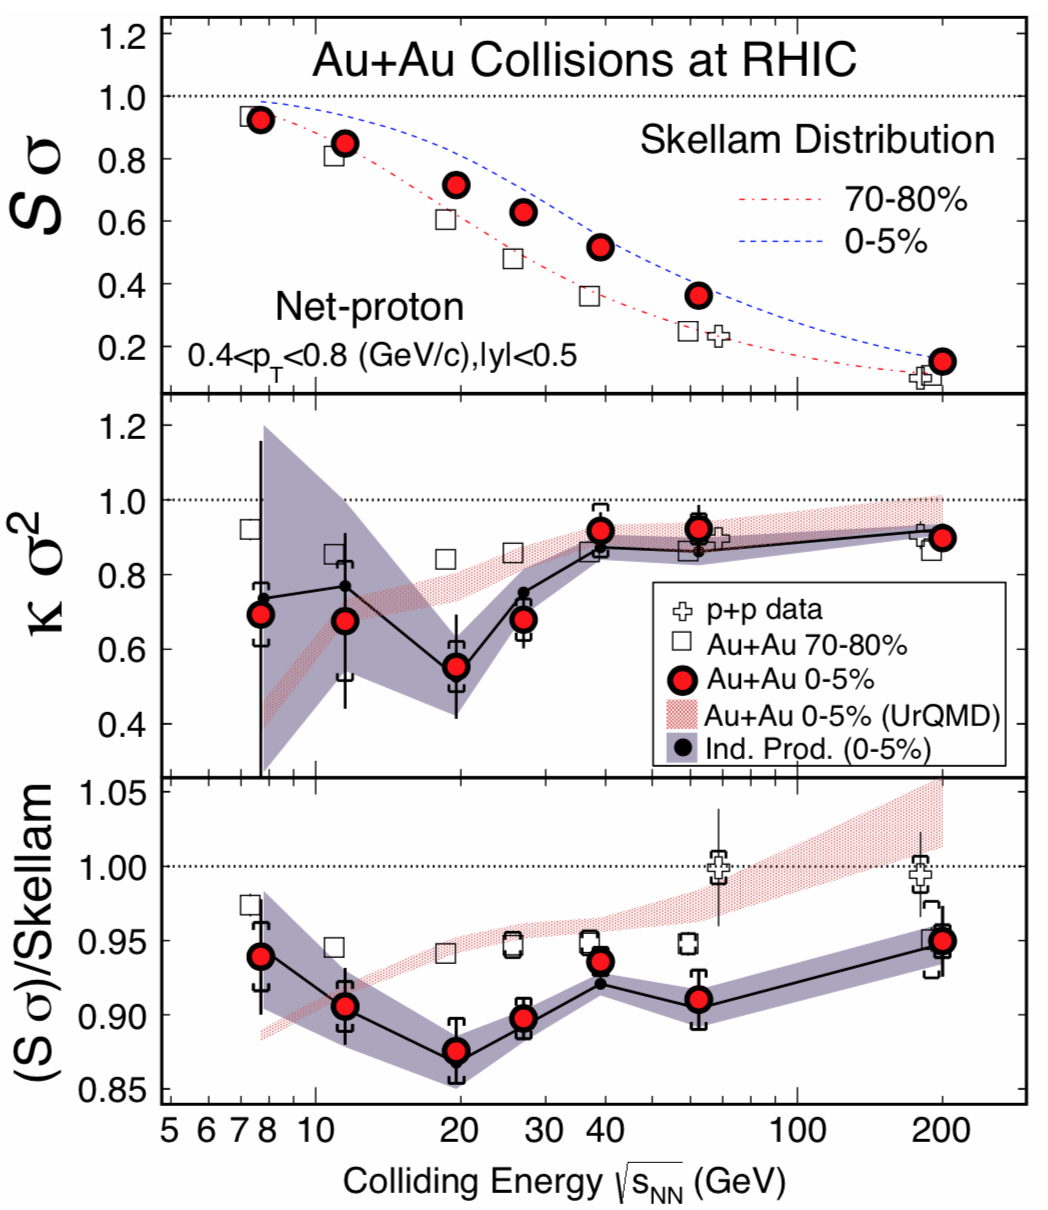
\includegraphics[width=.5\linewidth]{figs/chapter_intro/CP_STAR.png}
\caption{Collision energy and centrality dependence of the net-proton $S\sigma$ and $\kappa\sigma^2$ from Au+Au and $pp$ collisions at RHIC. Skellam distributions for corresponding collision centralities are shown in the top panel. This figure is taken from Ref.~\cite{Adamczyk:2013dal}.}
\label{fig:intro_CP_STAR}
\end{figure}



\subsubsection{Hanbury Brown and Twist (HBT)}

HBT correlations, which probe the space-time extent of a particle-emitting source, may provide valuable insights into the QGP source~\cite{Aaboud:2017xpw}. The HBT method originated in astronomy~\cite{HanburyBrown:1956bqd}, where space-time correlations of photons due to wave function symmetrization are used to measure the size of distant stars. The procedure can be adapted to the extremely small sources encountered in hadronic collisions if identical-particle Bose-Einstein correlations are instead studied in relative momentum space. In a typical HBT analysis, the two-particle correlation functions are fit to a function of relative momentum that is often a Gaussian or exponential function. The parameters of the fits that relate to the space-time extent of the source function are referred to as the HBT radii.

Invariant radii $R_\text{inv}$ are shown for several centralities in Figure~\ref{fig:intro_HBT_ATLAS} as a function a function of the cube root of average $d\Nch / d\eta$~\cite{Aaboud:2017xpw}. For both $k_\text{T}$ intervals shown, the scaling of $R_\text{inv}$ with $\lr{d\Nch / d\eta}^{1/3}$ is close to linear but with a slightly increasing slope at higher multiplicities. This observation is consistent with the prediction that the size of the QGP source should increase with the average multiplicity $d\Nch / d\eta$. In addition, the invariant radius has a steeper trend versus multiplicity at lower $k_\text{T}$. For a more complete review on HBT in heavy-ion collisions, refer to Ref.~\cite{Lisa:2005dd}.

\begin{figure}[H]
\centering
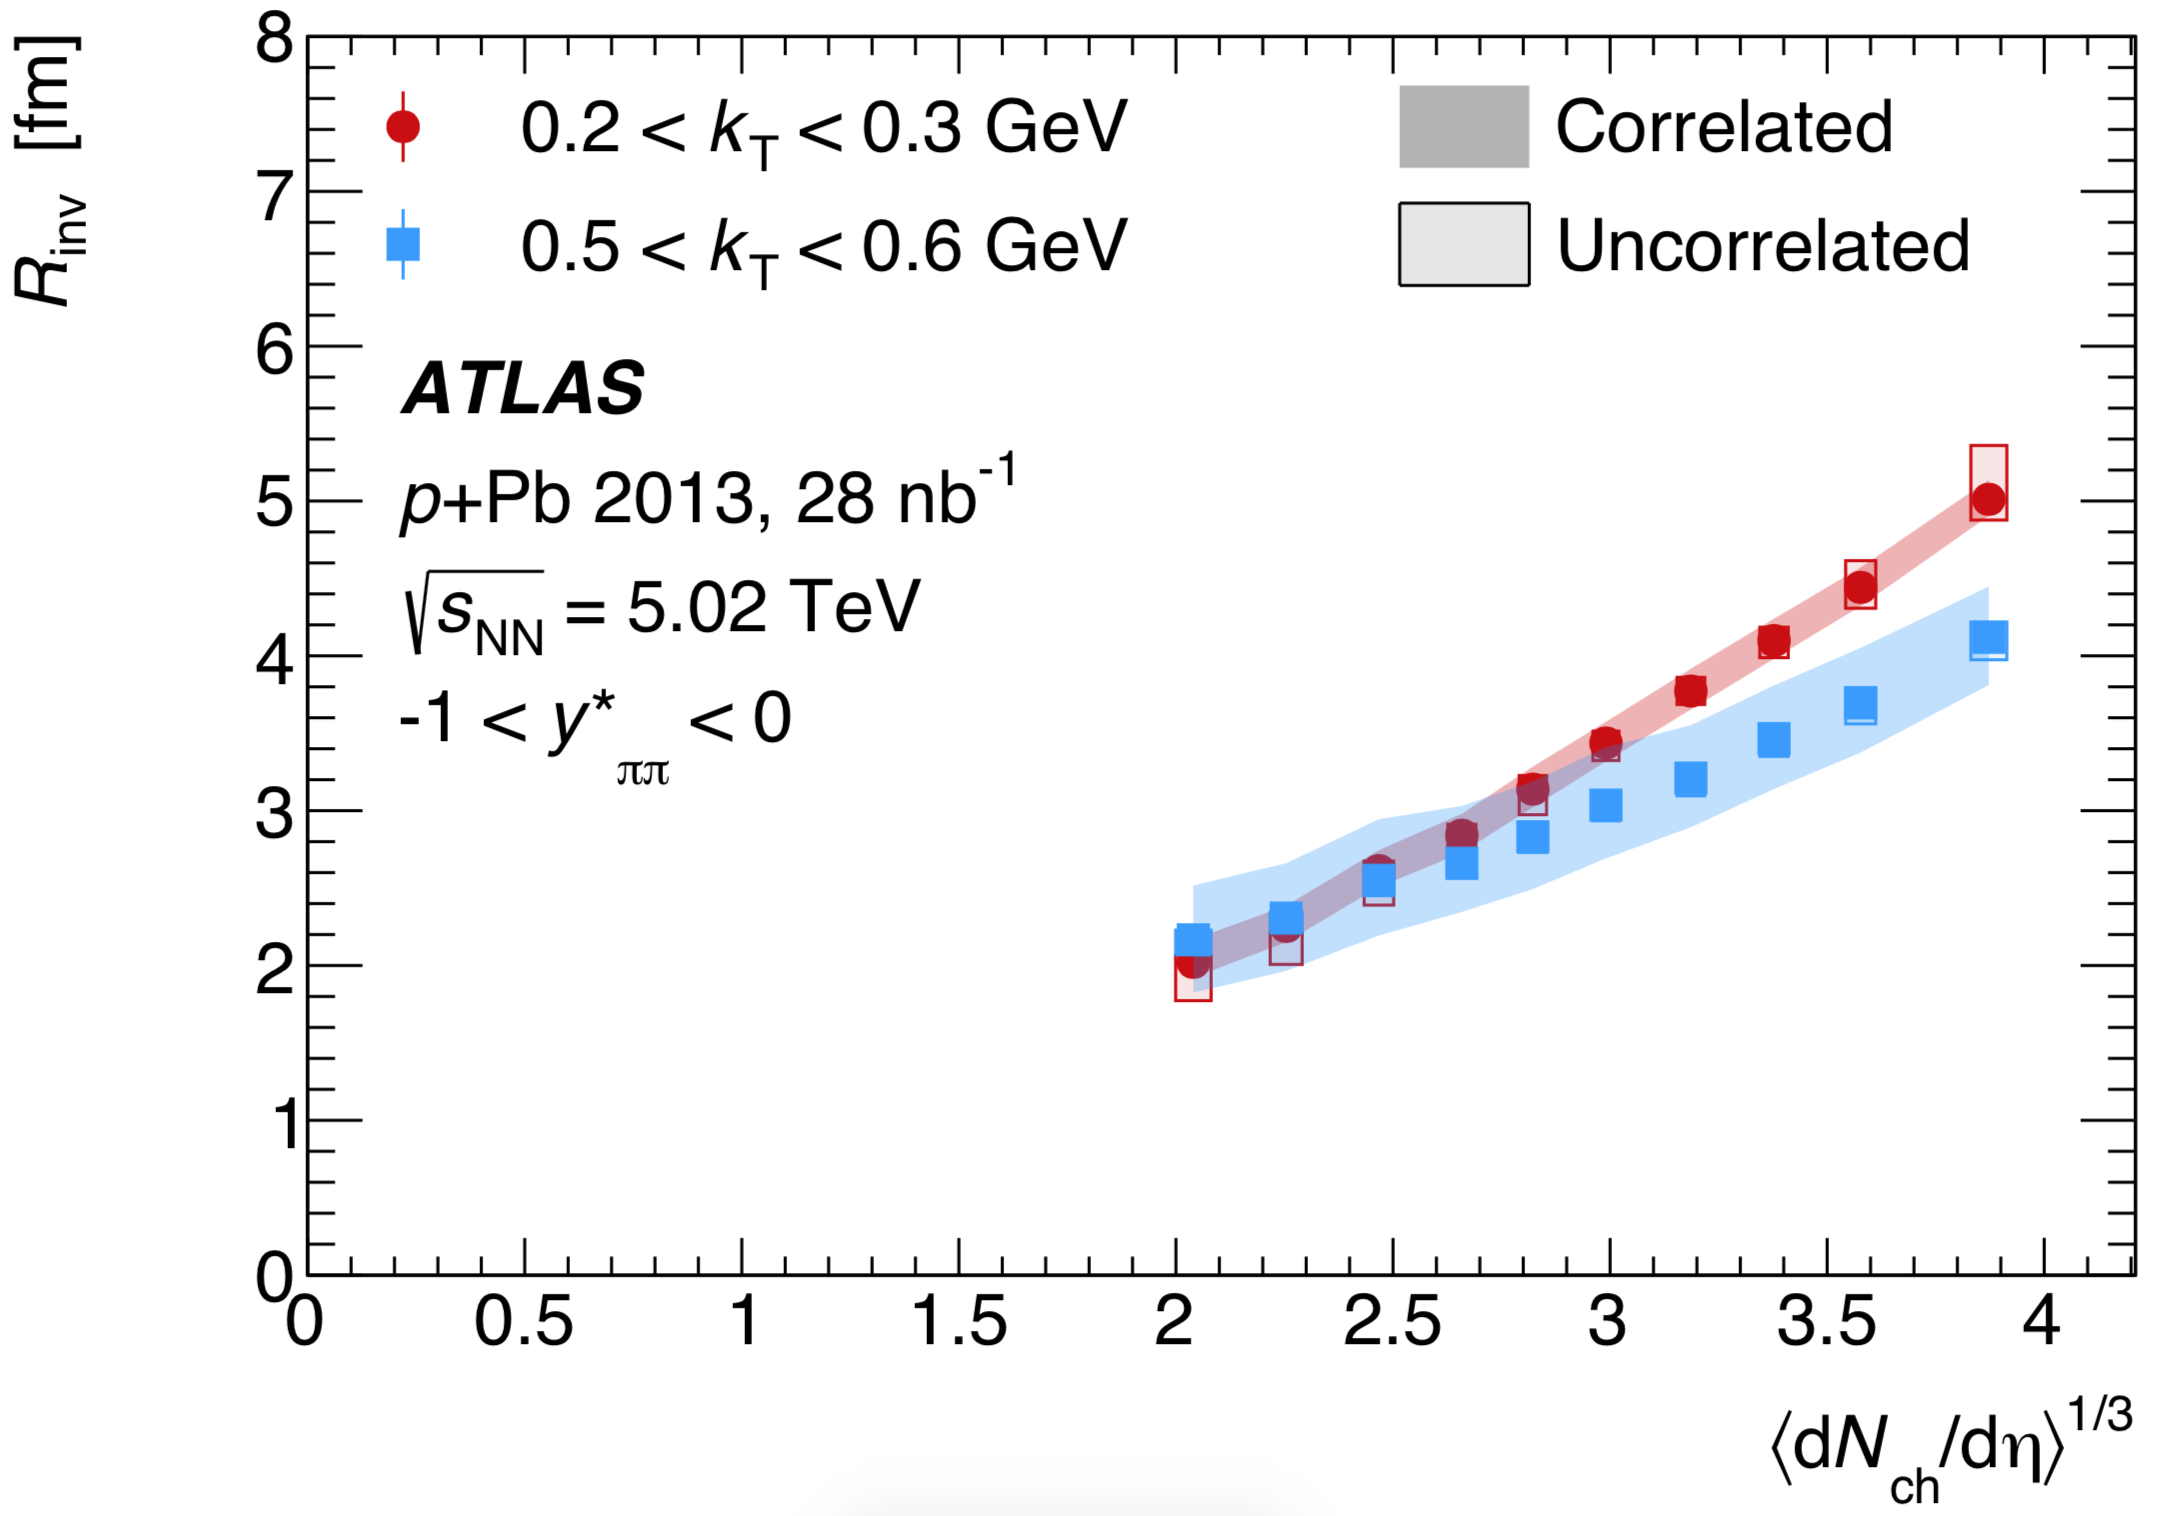
\includegraphics[width=.6\linewidth]{figs/chapter_intro/HBT_ATLAS.png}
\caption{Exponential fit results for Invariant radii $R_\text{inv}$ as a function of the cube root of average charged-particle multiplicity $\lr{d\Nch / d\eta}^{1/3}$, where the average is taken over $|\eta|<1.5$. This figure is taken from Ref.~\cite{Aaboud:2017xpw}.}
\label{fig:intro_HBT_ATLAS}
\end{figure}



\subsection{Motivation of this dissertation}

QGP produced in the HI collisions is unstable and will decay into stable particles that can be observed by detectors. By measuring distribution and event-by-event fluctuation of final stage particles, we could learn the initial stage conditions before the generation of QGP, and the hydrodynamical nature of the QGP expansion. Among all the final stage observables, flow is a fundamental observable to probe the initial spatial anisotropy and the fireball evolution. In this dissertation, we will provide new insights to the current understanding of flow by measuring the multiplicity and flow fluctuation in both transverse and longitudinal directions. In this section, an overview of present status of the flow measurements, as well as the challenges, are presented.



\subsubsection{Measurements in the transverse plane}
\label{sec:transverse_measurements}

The non-uniform initial geometry of the collision zone leads to an azimuthal anisotropy in the profile of the produced particles. The eccentricities in the initial geometry profile would eventually evolve to azimuthal anisotropy for the collision products. Currently there are many aspects of flow measurements in the transverse direction, each trying to address different problems.

\begin{itemize}
\item \textbf{Triangle flow and beyond} In the early days of the flow analysis, due to the "almond-like" shape of the overlap nucleus, elliptic flow ($v_2$) was thought to be dominating the transverse anisotropy. It was later realized that on the event-by-event basis, the initial geometry is not smooth but fluctuates around the average elliptic shape due to random positions of participated nucleons. Triangle flow ($v_3$), and even quadruple flow ($v_4$) provide important constrains on the fluctuations of the initial stage. One challenge in measuring $v_3$ and $v_4$ is that their signal strength are much smaller than the $v_2$. By utilizing the full statistics cumulated over the past few years of LHC, we are able to obtain high precise measurements of $v_3$ and $v_4$ in this dissertation. Refer to Section~\ref{sec:flow_cumulants_for_pvn} for details.
\item \textbf{Correlation between flow harmonics} In the early studies it was regularly assumed that the harmonics $v_n$ respond linearly to the eccentricities $\epsilon_n$ of the same order. However, recent studies argue that a relationship between event-by-event fluctuations of amplitudes of two different flow harmonics $v_n$ and $v_m$ can exist. In this dissertation, we investigated the correlations between $v_2$ and $v_3$, as well as $v_2$ and $v_4$. Refer to Section~\ref{sec:flow_cumulants_for_pvnvm} for details.
\item \textbf{Multi-particle nature of collective flow} An important question about the particle correlation measurements is whether it involves all particles in the event or if it is arises merely from correlations among a few particles. Since collective flow is intrinsically a multi-particle phenomenon, it can be probed more directly using cumulants based on multi-particle correlation techniques. We studied azimuthal correlations involving four and six particles in multiple collision systems. Refer to Section~\ref{sec:flow_cumulants_for_pvn} for details.
\item \textbf{$\pT$ dependence of multi-particle correlations} Another factor that breaks the $v_n \propto \epsilon_n$ is the hydrodynamical evolution and final state effects. Hydrodynamic model calculations suggest strong $\pT$-dependent fluctuations of $v_n$ even in a single event. Such final-state intra-event flow fluctuations may change $v_n$ in a $\pT$ dependent way, and can be quantified by comparing $v_n$ measurements using particles in different $\pT$ ranges. In this dissertation, for each observable, we presented the results in multiple $\pT$ ranges. Refer to Section~\ref{sec:flow_cumulants_for_pvn} for details.
\item \textbf{System size dependence} Experimental data has implied values of $\eta/s$ close to $0.2$ at LHC energy, however, uncertainties in the modeling of the initial state have prevented the extraction of more precision information. The data from different collision systems with different nuclei sizes may provide an opportunity to further constrain $\eta/s$. Our studies utilized the new collected Xe+Xe data, and compared the flow results to previous measured Pb+Pb results. Various initial state models predict Xe+Xe and Pb+Pb collisions have similar values of $\epsilon_2$, therefore the ratios of Xe+Xe to Pb+Pb $v_2$ coefficients in the mid-centrality range could be directly sensitive to $\eta/s$. Refer to Section~\ref{sec:novel_collision_systems_xexe} for details.
\item \textbf{Smallest QGP droplet} Many flow and other measurements have shown that QGP might exist in ion-ion collisions. In recent years, two-particle flow correlation shows hints of elliptic flow in the small systems like proton-proton and proton-lead. To confirm previous observation, we have developed special triggers to collect enough $pp$ events in the high multiplicity region. The four-particle cumulants we measured shows a negative sign that supports the collective phenomenon in the small systems. Our new results contributed to the discussions in search for the smallest QGP droplet produced in the experiment. Refer to Section~\ref{comparison_between_different_cumulant_methods} for details. (For a review of collectivity in small systems, refer to Ref.~\cite{Nagle:2018nvi}.)
\item \textbf{Background suppression} Depending on the signals we are interested in, there are many backgrounds that need to be suppressed. In the flow measurements, one of the most significant background arises from particle correlations among a few particles, due to resonance decays, jets, or multi-jet production (non-flow). Non-flow is especially significant in smaller collision systems and we have developed a novel subevent algorithm to effectively remove such background. Another important background originates from our limited access to the initial stage quantities such as number of participating nucleons $N_\text{part}$. Since centrality defined in experiment is only an estimate of $N_\text{part}$ on the average level, the fluctuation of centrality will have an impact on all the fluctuations measurements. In this dissertation, we also spent some efforts investigating such effect in flow cumulant measurements. Refer to Section~\ref{sec:subevent_cumulant_method} and Section~\ref{sec:glauber_model} for details.
\end{itemize}



\subsubsection{Measurements in the longitudinal direction}

Before the collision of nucleus, the number of nucleon participants in the target and projectile fluctuate from event-to-event. This longitudinal fluctuation directly affects the entropy production at very early time of the collision, well before the onset of the collective flow. Experimental measurements provide a window into the space-time picture of the collective expansion as well as the medium properties that drives the expansion.

Longitudinal correlations have been measured extensively in previous studies, however, many questions still remain to be addressed. There are currently two majors areas for longitudinal measurements:
\begin{itemize}
\item \textbf{Multiplicity correlation} To study the early-time density fluctuations in pseudorapidity, forward-backward correlations of particle multiplicity in two $\eta$ ranges were measured in many collision systems. Instead of using limited information, we proposed a more general and comprehensive method by decomposing the correlation function into orthogonal Legendre polynomial functions (or into principal components as suggested by others), each representing a unique component of the measured forward-backward correlation. Furthermore, we developed a data-driven method to suppress the multiplicity correlations from the final state such as resonance decays, single-jet fragmentation, and Bose-Einstein correlations. In this dissertation, our new methods were applied from large to small collision systems. Refer to Section~\ref{sec:fb_atlas_data} for details.
\item \textbf{Flow decorrelation} Most previous flow studies assumed that the initial condition and space-time evolution of the matter are boost-invariant in the longitudinal direction. Recent model studies of two-particle correlations as a function of pseudorapidity $\eta$ revealed strong event-by-event fluctuations of the flow magnitude and phase between two well-separated pseudorapidities, named as flow decorrelation. Even though in this dissertation we do not measure flow decorrelation directly, we will have brief discussions on this topic when introducing the subevent technique. Refer to Section~\ref{sec:flow_decorrelation} for details.
\end{itemize}



\subsection{Outline of this dissertation}

In the first half of Section~\ref{chapter:detector}, we will introduce the setup of Large Hadron Collider and describe all the sub-detectors of the ATLAS detector that have been used in our measurements. In the second half of Section.~\ref{chapter:detector}, we will explain how the data (Pb+Pb, Xe+Xe, $p$+Pb and $pp$) were gathered and cleaned. Track selection and reconstruction procedures are also discussed in this section.

In Section~\ref{chapter:fbcorr}, we will present the longitudinal multiplicity correlation measurements, using HIJING and AMPT models, as well as the ATLAS data. We will first discuss the limitations of previous analyses, and then introduce a new observable to dissect longitudinal dynamics. A data-driven technique to suppression background is explained. After presenting the results in models and data, we will summarize and discuss the potential improvements on the measurements.

In Section~\ref{chapter:subcumu}, we will present the subevent flow cumulant studies, using PYTHIA model and the ATLAS data. We will first point out that the standard cumulant method suffers from non-flow background, then the state-of-the-art subevent algorithm is introduced and validated in model. After applying the new method successfully to ATLAS data, we will also discuss the extension of this new method to other measurements.

In Section~\ref{chapter:centfluc}, we will present the flow and centrality fluctuation studies, using Glauber model and ATLAS data. First, we will explain what is centrality fluctuation and how to measure it in a simple Glauber model. Then we will explain how to qualitatively measure this effect in a model-independent way. Different collision system, Xe+Xe, will also be covered at the end of this section.

In Section~\ref{chapter:summary}, we will review all the puzzles and challenges we mentioned in the introduction section, then summarize how the studies in this dissertation help to answer those questions.

In the Appendix~\ref{chapter:appendix}, two technical aspects of our studies will be discussed: first is how to develop an algorithm to speed up the multi-particle cumulant calculation; second is a walk-through of estimating the systematic uncertainties in these measurements.













\newpage
{\bf\huge{Chapter 2}\par}
\section{The ATLAS detector and data taking}
\label{chapter:detector}

The Large Hadron Collider (LHC)~\cite{Evans:2008zzb} at CERN is currently the world's newest, largest and most powerful collider, located near Geneva, Switzerland. It is designed to collide proton-proton with a center of mass of 14 TeV and an unprecedented luminosity of $10^{-34}\text{cm}^{-2}\text{s}^{-1}$. It can also collide heavy ions, like Pb+Pb and Xe+Xe, with an energy of several TeV per nucleon and a peak luminosity of $10^{-27}\text{cm}^{-2}\text{s}^{-1}$. In this section, we aim to describe the designs of LHC and ATLAS detector, as well as the data acquisition and selection procedure.

\subsection{The Large Hadron Collider}

The LHC~\cite{Evans:2008zzb} is a two-ring-superconducting-hadron accelerator and collider installed in the existing 26.7 km tunnel that was constructed between 1984 and 1989 for the CERN LEP machine. The LEP tunnel has eight straight sections and eight arcs and lies between 45 m and 170 m below the surface on a plane inclined at $1.4\%$ sloping. LHC contains two counter-propagating beams containing bunches of protons or ions that cross each other at four points, where collisions take place. At these crossing points, located four LHC detectors: ATLAS, CMS, ALICE and LHCb. ALICE is specially designed for the heavy-ion program, while ATLAS and CMS are mainly targeted for proton collisions, and will collect heavy-ion data for about one month each year. The bending power for the beams is provided by 1232 superconducting dipole magnets, each 15 m long and capable of generating 8.3 T magnetic fields. To focus the beam, quadrupole magnets are implemented. Accelerating cavities are used to compensate for the energy loss and keep the bunches at a constant energy.

In Run 2, Pb ion can achieve the energy up to 5.02 TeV per nucleon. Ions are boosted in a sequence of accelerators before injected into the LHC. An example of the sequence is shown in Figure~\ref{fig:detector_cartoon_LHC}, where Pb ions go through LINAC3, LEIR, PS, SPS and LHC, with the energy being ramped up at each stage: 4.2 MeV, 72 MeV, 6 GeV, 177 GeV and 2.76 TeV.

\begin{figure}[H]
\centering
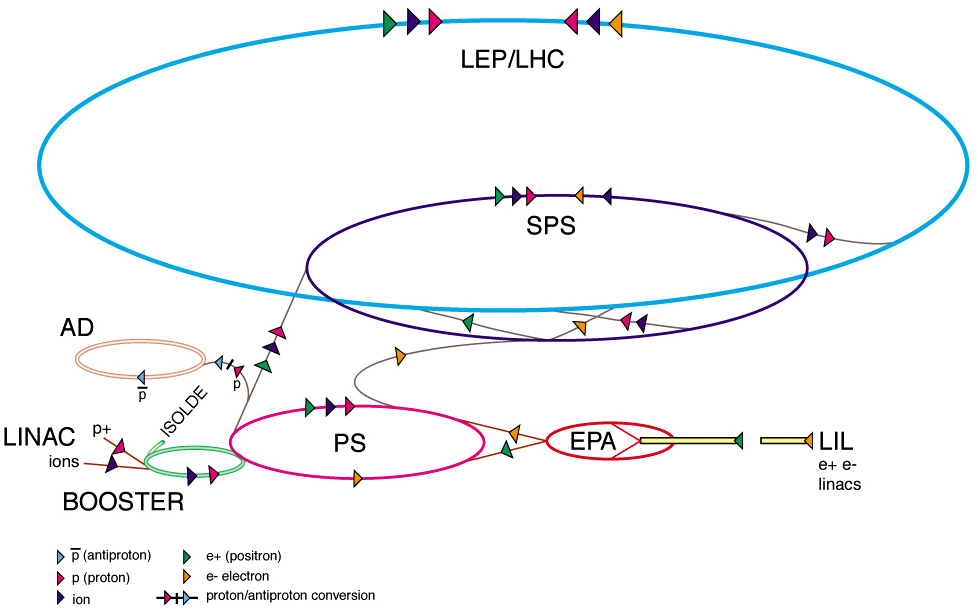
\includegraphics[width=.95\linewidth]{figs/chapter_detector/cartoon_LHC.jpg}
\caption{The CERN accelerator sequence. The figure is taken from Ref.~\cite{Jean-Luc:841493}.}
\label{fig:detector_cartoon_LHC}
\end{figure}



\subsection{The ATLAS detector}

The physics goals of heavy-ion program can be turned into a set of general requirements for the LHC detectors:
\begin{itemize}
\item Due to the experimental conditions, the detectors require fast, radiation-hard electronics and sensor elements.
\item High detector granularity is needed to handle the particle fluxes and to reduce the influence of overlapping events;
\item Large acceptance in pseudorapidity with almost full azimuthal angle coverage is required;
\item Good charged particle momentum resolution and reconstruction efficiency in the inner tracker are essential;
\item Highly efficient triggering on low transverse-momentum objects with sufficient background rejection;
\end{itemize}

ATLAS (A Toroidal LHC ApparatuS)~\cite{Aad:2008zzm} is a multi purpose detector located at Point-1 of the LHC cavern. While mainly designed to study the $pp$ collisions, its fine granularity and large acceptance makes it an ideal detector for study Pb+Pb and $p$Pb collisions as well. The overall ATLAS detector layout is shown in Figure~\ref{fig:detector_ATLAS_detector}. The ATLAS detector is nominally forward-backward symmetric with respect to the interaction point, and covers the full azimuthal angle. The magnet configuration comprises a thin superconducting solenoid surrounding the inner-detector cavity, and three large superconducting toroids (one barrel and two end-caps) arranged with an eight-fold azimuthal symmetry around the calorimeters. This fundamental choice has driven the design the rest of the detector. In this section, only the subsystems that are used in this work are described:
\begin{itemize}
\item Inner Detector (ID);
\item Forward Calorimeter (FCal);
\item Zero-Degree Calorimeter (ZDC);
\item Minimum-Bias Trigger Scintillators (MBST);
\end{itemize}

\begin{figure}[H]
\centering
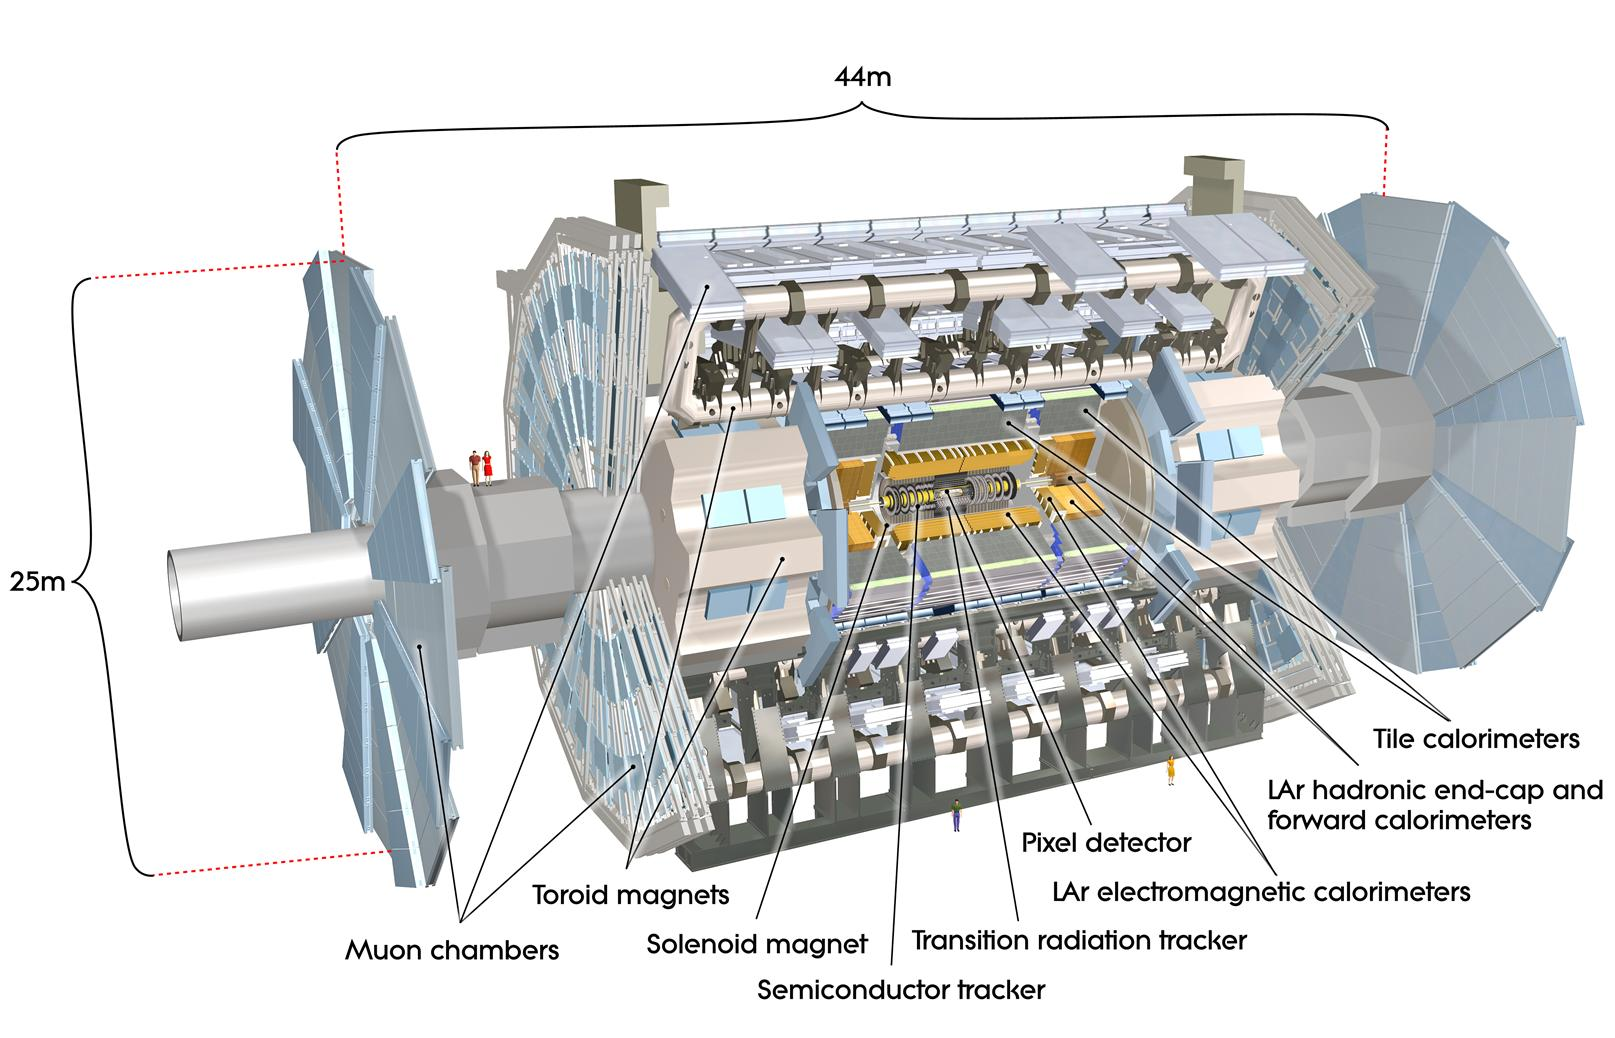
\includegraphics[width=.95\linewidth]{figs/chapter_detector/ATLAS_detector.jpg}
\caption{Cut-away view of the ATLAS detector. The dimensions of the detector are 25 m in height and 44 m in length. The overall weight of the detector is approximately 7000 tonnes.}
\label{fig:detector_ATLAS_detector}
\end{figure}



\subsubsection{Inner Detector}

The ATLAS Inner Detector (ID)~\cite{Aad:2008zzm} is designed to provide hermetic and robust pattern recognition, excellent momentum resolution and both primary and secondary vertex measurements for charged tracks above a given $\pT$ threshold (nominally 0.5 GeV, but can go as low as 0.1 GeV in some cases) and within the pseudorapidity range $|\eta|<2.5$. The ID layout, as shown in Figure~\ref{fig:detector_ATLAS_ID}, reflects the performance requirements. The ID is contained within a cylindrical envelope of 7 m and of radius 1.2 m, within a solenoidal magnetic field of 2 T.

\begin{figure}[H]
\centering
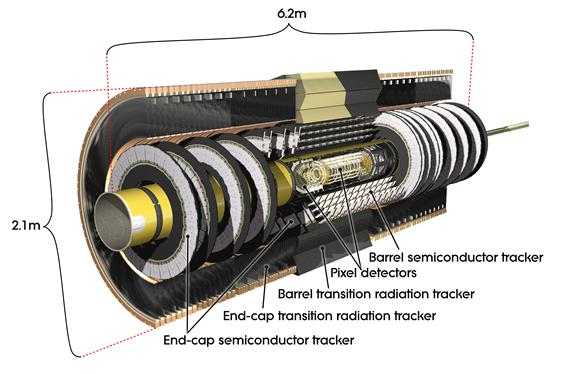
\includegraphics[width=.95\linewidth]{figs/chapter_detector/ATLAS_ID.jpg}
\caption{Cut-away view of the ATLAS Inner Detector. The ID is contained within a cylindrical envelope of length 7 m and of radius 1.2 m, within a solenoidal magnetic field of 2 T.}
\label{fig:detector_ATLAS_ID}
\end{figure}

The ID consists of three independent but complementary sub-detectors. At inner radii, high-resolution pattern recognition capabilities are available using discrete space-points from silicon Pixel layers and stereo pairs of silicon micro-strip (SCT) layers. At large radii, the transition radiation tracker (TRT) comprises many layers of gaseous straw tube elements interleaved with transition radiation material. Pixel, SCT and TRT sub-detectors will be described below separately.



\paragraph{Pixel}

The pixel~\cite{Aad:2008zz} detector is the innermost element of the Inner Detector as shown in Figure~\ref{fig:detector_ATLAS_ID}. The pixel tracker is designed to provide at least three points on a charged track emanating from the collision region. The principle components of the pixel tracking system are the following:
\begin{itemize}
\item The active region of the pixel detector, which is composed of three barrel layers and a total of six disk layers, three at each end of the barrel region;
\item Internal services and their associated mechanical support structures on both ends of the active detector region;
\item A pixel support tube into which the active part of the pixel detector and the services and related support structures are inserted and located;
\item External services that are connected to the internal services at the end of the pixel support tube.
\end{itemize}

The active region of the pixel detector is shown in a schematic view in Figure~\ref{fig:detector_ATLAS_ID_pixel}. The active part of the pixel system consists of three barrel layers: Layer 0, Layer 1 and Layer 2, and two identical endcap regions, each with three disk layers. The basic building block of the active part of the pixel detector is a module that is composed of silicon sensors, front-end electronics and flex-hybrids with control circuits. All modules are functionally identical at the sensor/integrated circuit level, but different somewhat in the interconnection schemes for barrel modules and disk modules. The nominal pixel size is 50 microns in the $\phi$ direction and 400 microns in $z$ (beam axis) and $r$ (disk region). There are 46080 pixel electronics channels in a module. The total number of pixels in the system approximately 67 million in the barrel and 13 million in the endcaps, covering a total area of about 1.7 $\text{m}^2$.

\begin{figure}[H]
\centering
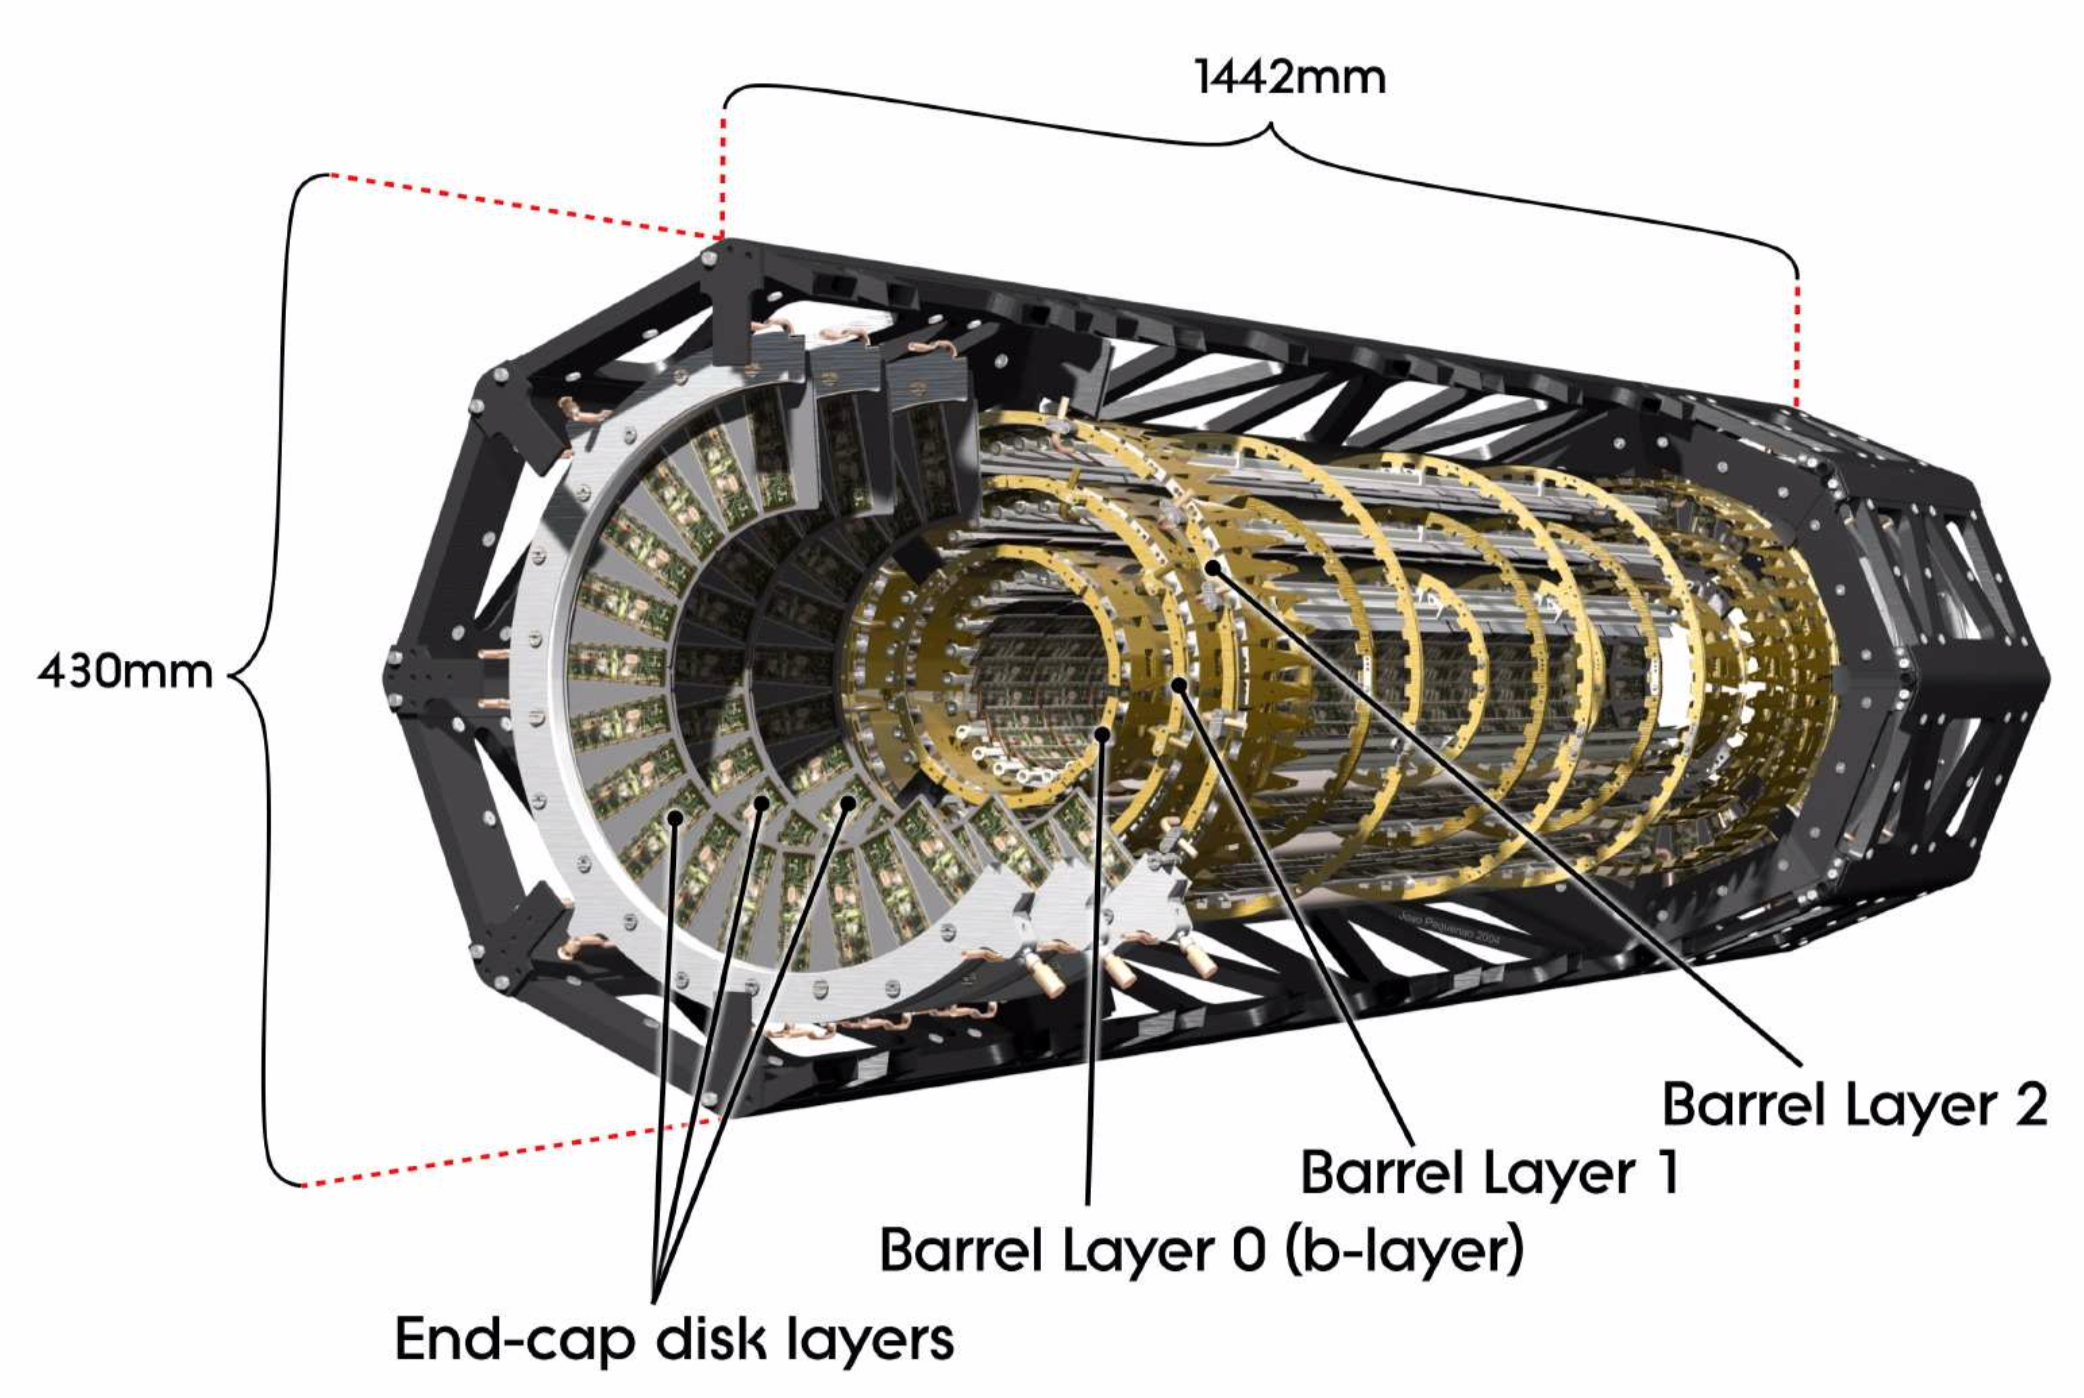
\includegraphics[width=.95\linewidth]{figs/chapter_detector/ATLAS_ID_pixel.png}
\caption{A schematic view of the active region of the pixel detector consisting of barrel and endcap layers.}
\label{fig:detector_ATLAS_ID_pixel}
\end{figure}

To get an idea of the number of pixel hits in different region, left panel of Figure~\ref{fig:detector_ATLAS_ID_pixel_hits} shows an average number of pixel hits per track as a function of pseudorapidity $\eta$. For $|\eta|<2.0$, the average pixel hits is around four, instead of three, which corresponds to the three barrel layers discussed above. This is because an additional pixel layer, the insertable B-layer (IBL), was installed between Run 1 (2010-2013) and Run 2 (2015-2018). This additional layer further increases the performance of tracking reconstruction. For $2.0<|\eta|<2.5$, the average pixel hits is larger, due to the additional endcap layers. The right panel of Figure~\ref{fig:detector_ATLAS_ID_pixel_hits} shows the distribution of number of pixel hits per track. It suggests that most tracks go through all the four barrel layers, while very few tracks could have pixel hits up to 7. The consistency between 2017 and 2015 means that the performance of pixel sub-detector is stable during the Run 2.

\begin{figure}[H]
\centering
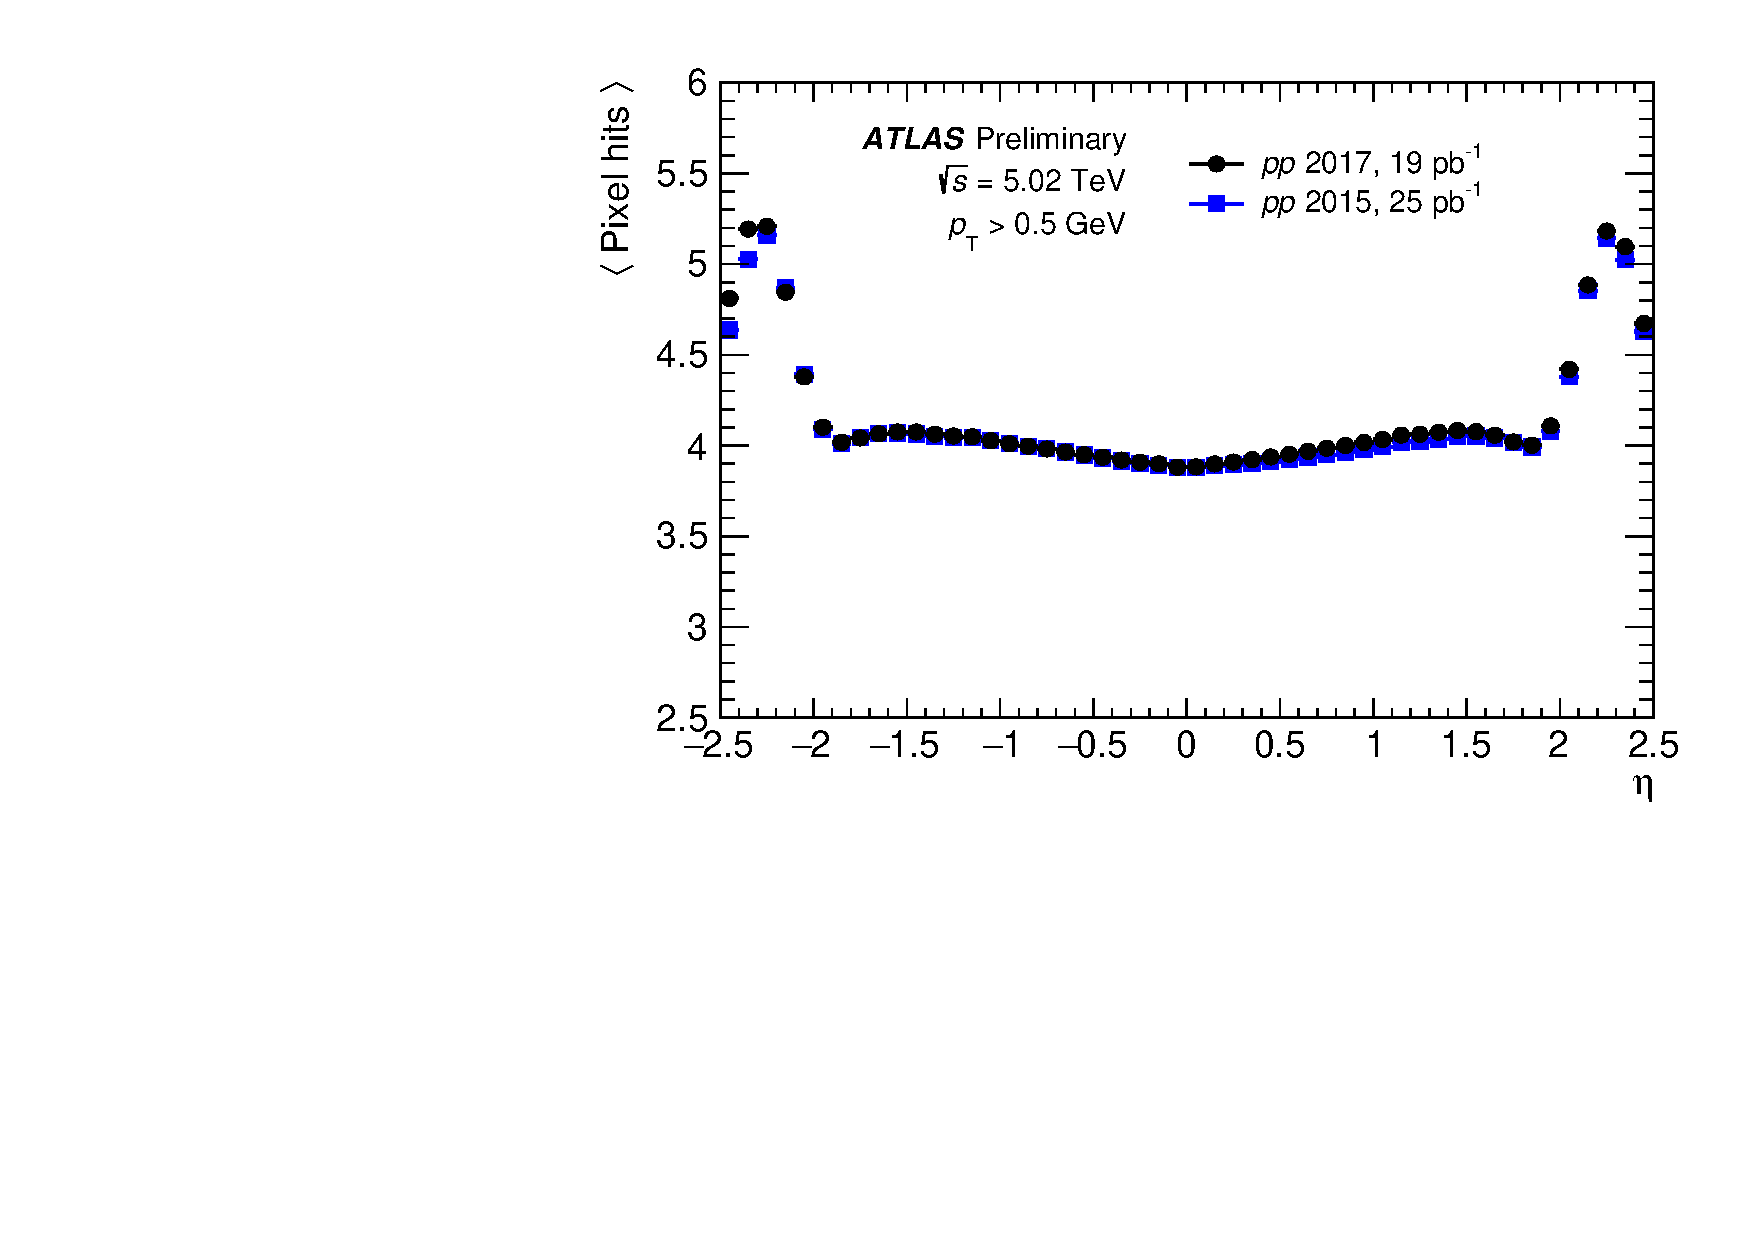
\includegraphics[width=.475\linewidth]{figs/chapter_detector/ATLAS_ID_pixel_hits1.pdf}
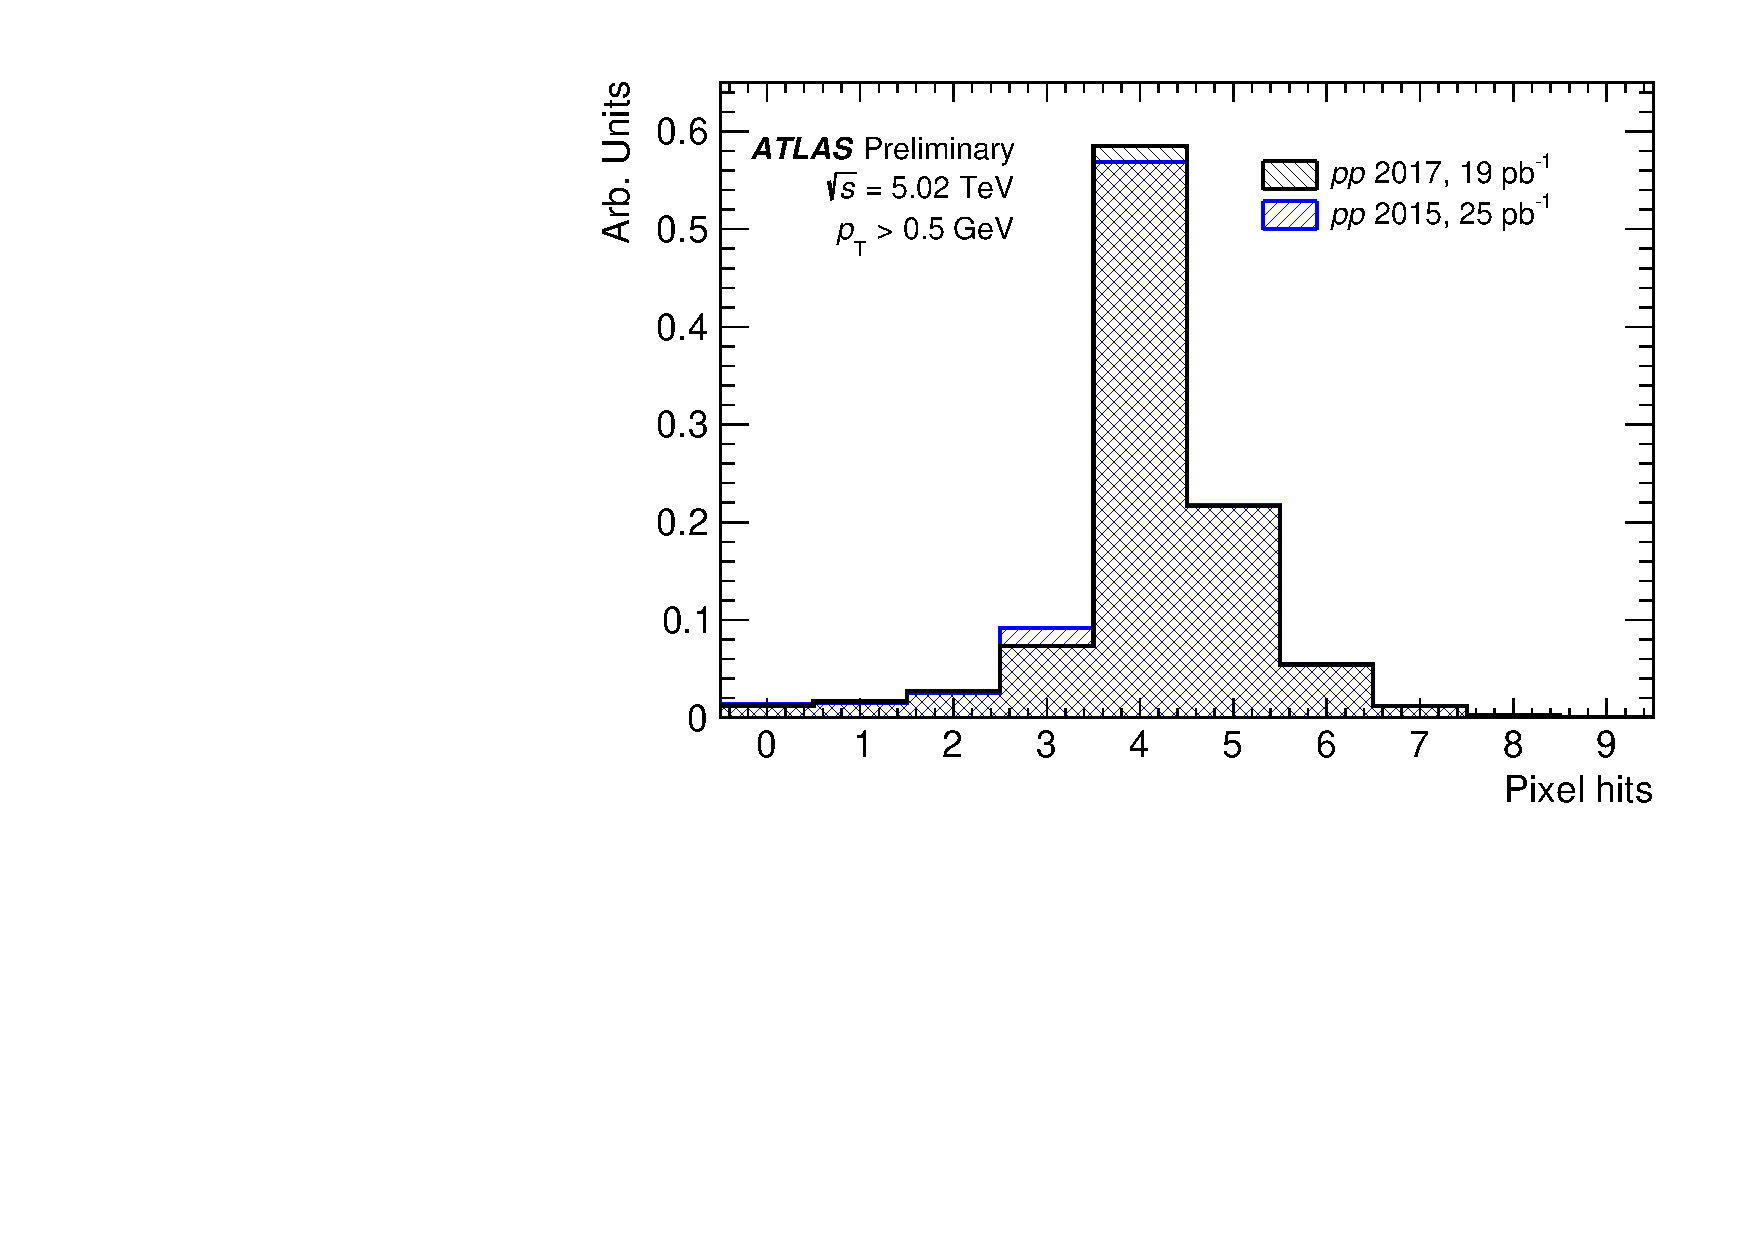
\includegraphics[width=.475\linewidth]{figs/chapter_detector/ATLAS_ID_pixel_hits2.pdf}
\caption{Left: an average number of pixel hits per track as a function of pseudorapidity. Right: a number of pixel hits per track. Tracks are required to have $\pT>0.5$ GeV. Events are required to have a reconstructed vertex.}
\label{fig:detector_ATLAS_ID_pixel_hits}
\end{figure}



\paragraph{SCT}

The SemiConductor Tracker (SCT)~\cite{Ahmad:2007zza} surround the pixel detector, and uses semiconductor technology to provide precision space-point coordinates. In the SCT there are four cylinders in the barrel and nine disks in each of the two endcaps, with every layer able to read out a position in two dimensions. There are in total 8448 identical rectangular single-sided $p$-in-$n$ sensors installed in the ATLAS barrel SCT and 6944 single-sided $p$-in-$n$ sensors, of five different wedge-shaped geometries, in the SCT endcaps. The micro strip sensors are assembled as part of barrel and endcap detection modules in the SCT. In most cases there are two single-sided sensors on each side of a module, glued back-to-back around a high thermal conductivity substrate. The sensor strips are AC-coupled to binary readout electronics, with the ABCD3TA custom ASIC~\cite{Campabadal:2005rj} providing the front-end amplification, discrimination, pipeline, de-randomisation and data compression functions. The layout of the barrel sensors within an SCT module is shown in Figure~\ref{fig:detector_ATLAS_ID_SCT}, together with modules mounted on a barrel.

\begin{figure}[H]
\centering
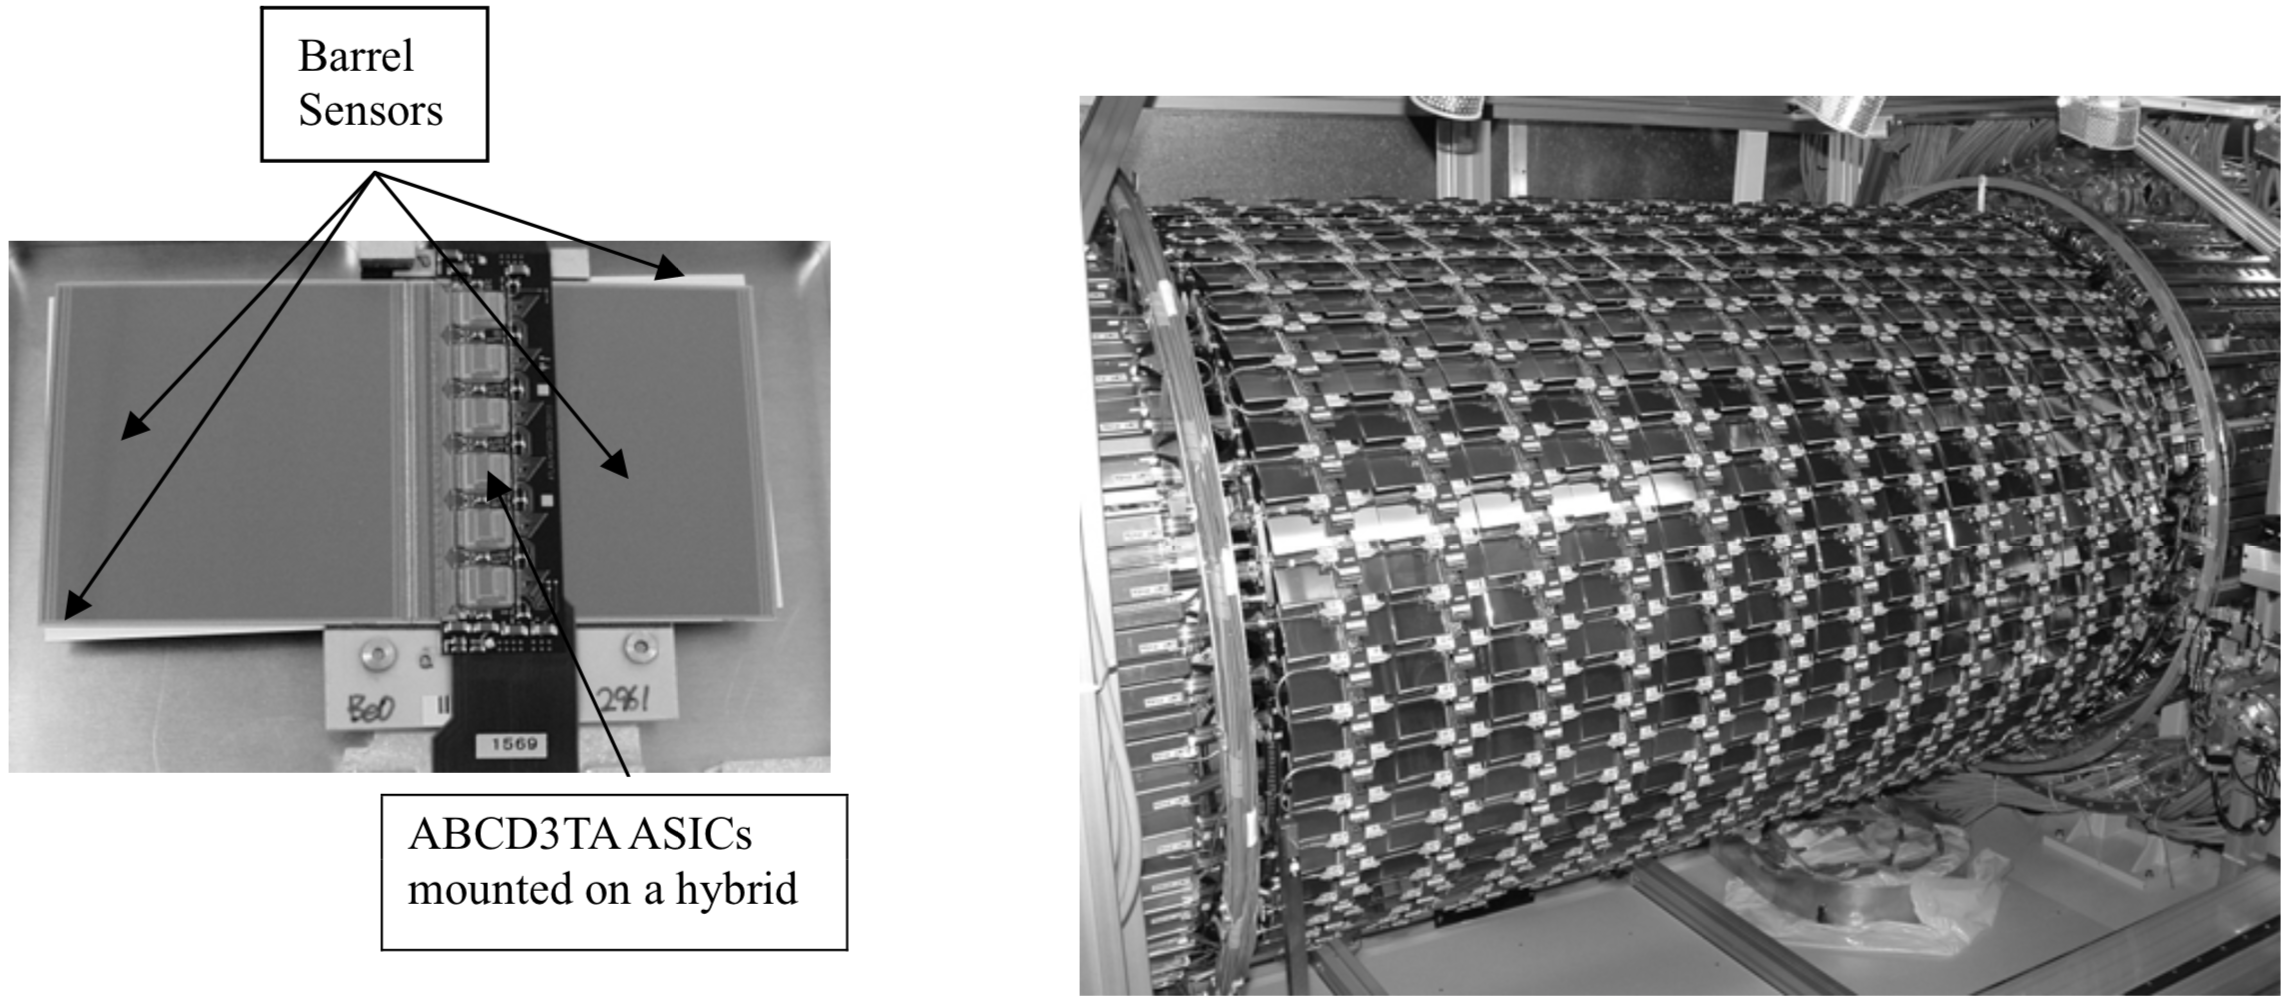
\includegraphics[width=.95\linewidth]{figs/chapter_detector/ATLAS_ID_SCT.png}
\caption{Left: Layout of the 4 sensors (2 on the upper surface, 2 on the lower surface, with 40 mrad stereo rotation) in the SCT barrel module. The readout ASICs are mounted on a hybrid, bridged over the sensors. Right: Modules mounted on the outermost of the 4 barrel structures of the ATLAS SCT.}
\label{fig:detector_ATLAS_ID_SCT}
\end{figure}

To get an idea of the number of hits per track in different regions of the SCT detector, left panel of Figure~\ref{fig:detector_ATLAS_ID_SCT_hits} shows an average number of SCT hits as a function of pseudorapidity $\eta$. For $|\eta|<1.5$, the average SCT hits is around 8, which corresponds to the four cylinders (2 sensors on each side) in the barrel region. For $1.5<|\eta|<2.5$, the average SCT hits is larger, due to additional 9 endcap disks. The right panel of Figure~\ref{fig:detector_ATLAS_ID_SCT_hits} shows the distribution of number of SCT hits per track. The number of hits for most track is between 8 and 10. The consistency between 2017 and 2015 indicates that the performance of SCT is stable during the Run 2.

\begin{figure}[H]
\centering
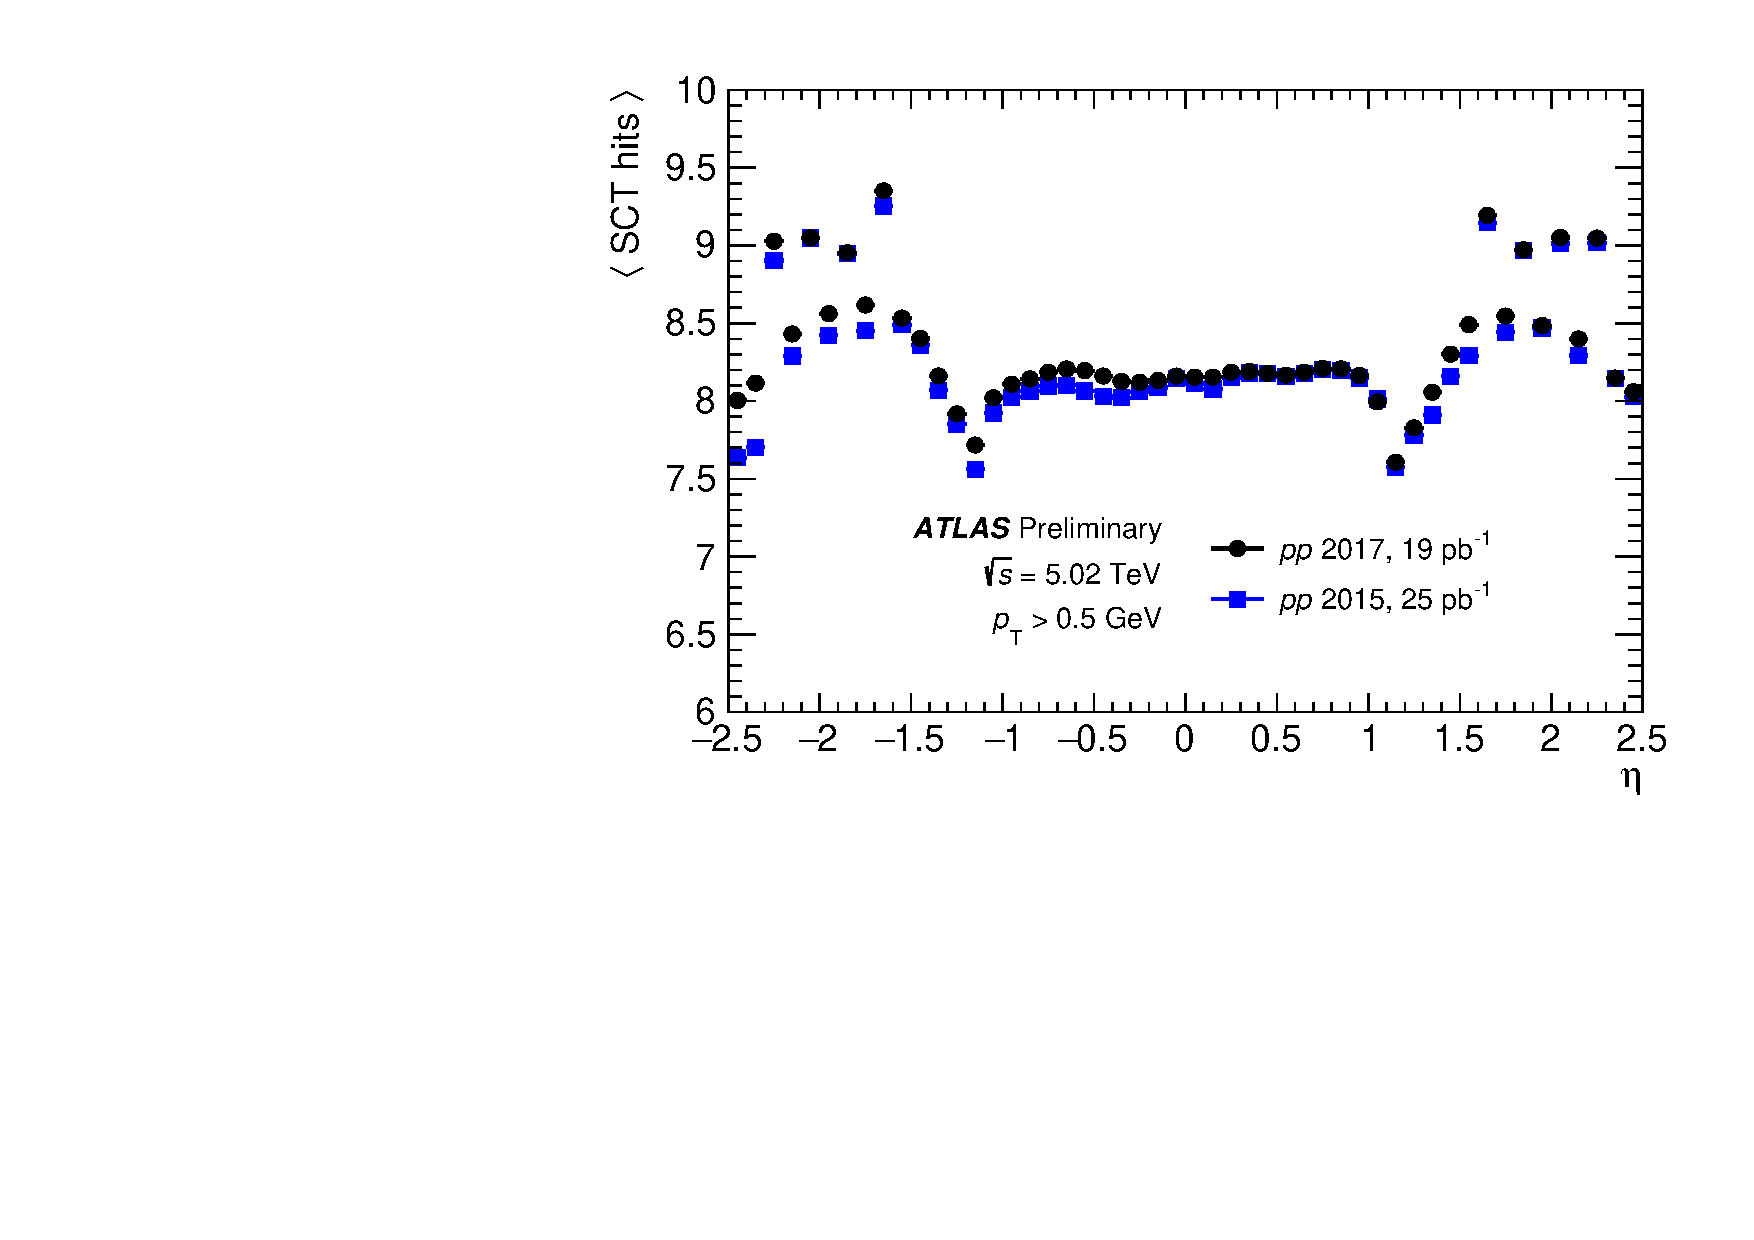
\includegraphics[width=.475\linewidth]{figs/chapter_detector/ATLAS_ID_SCT_hits1.pdf}
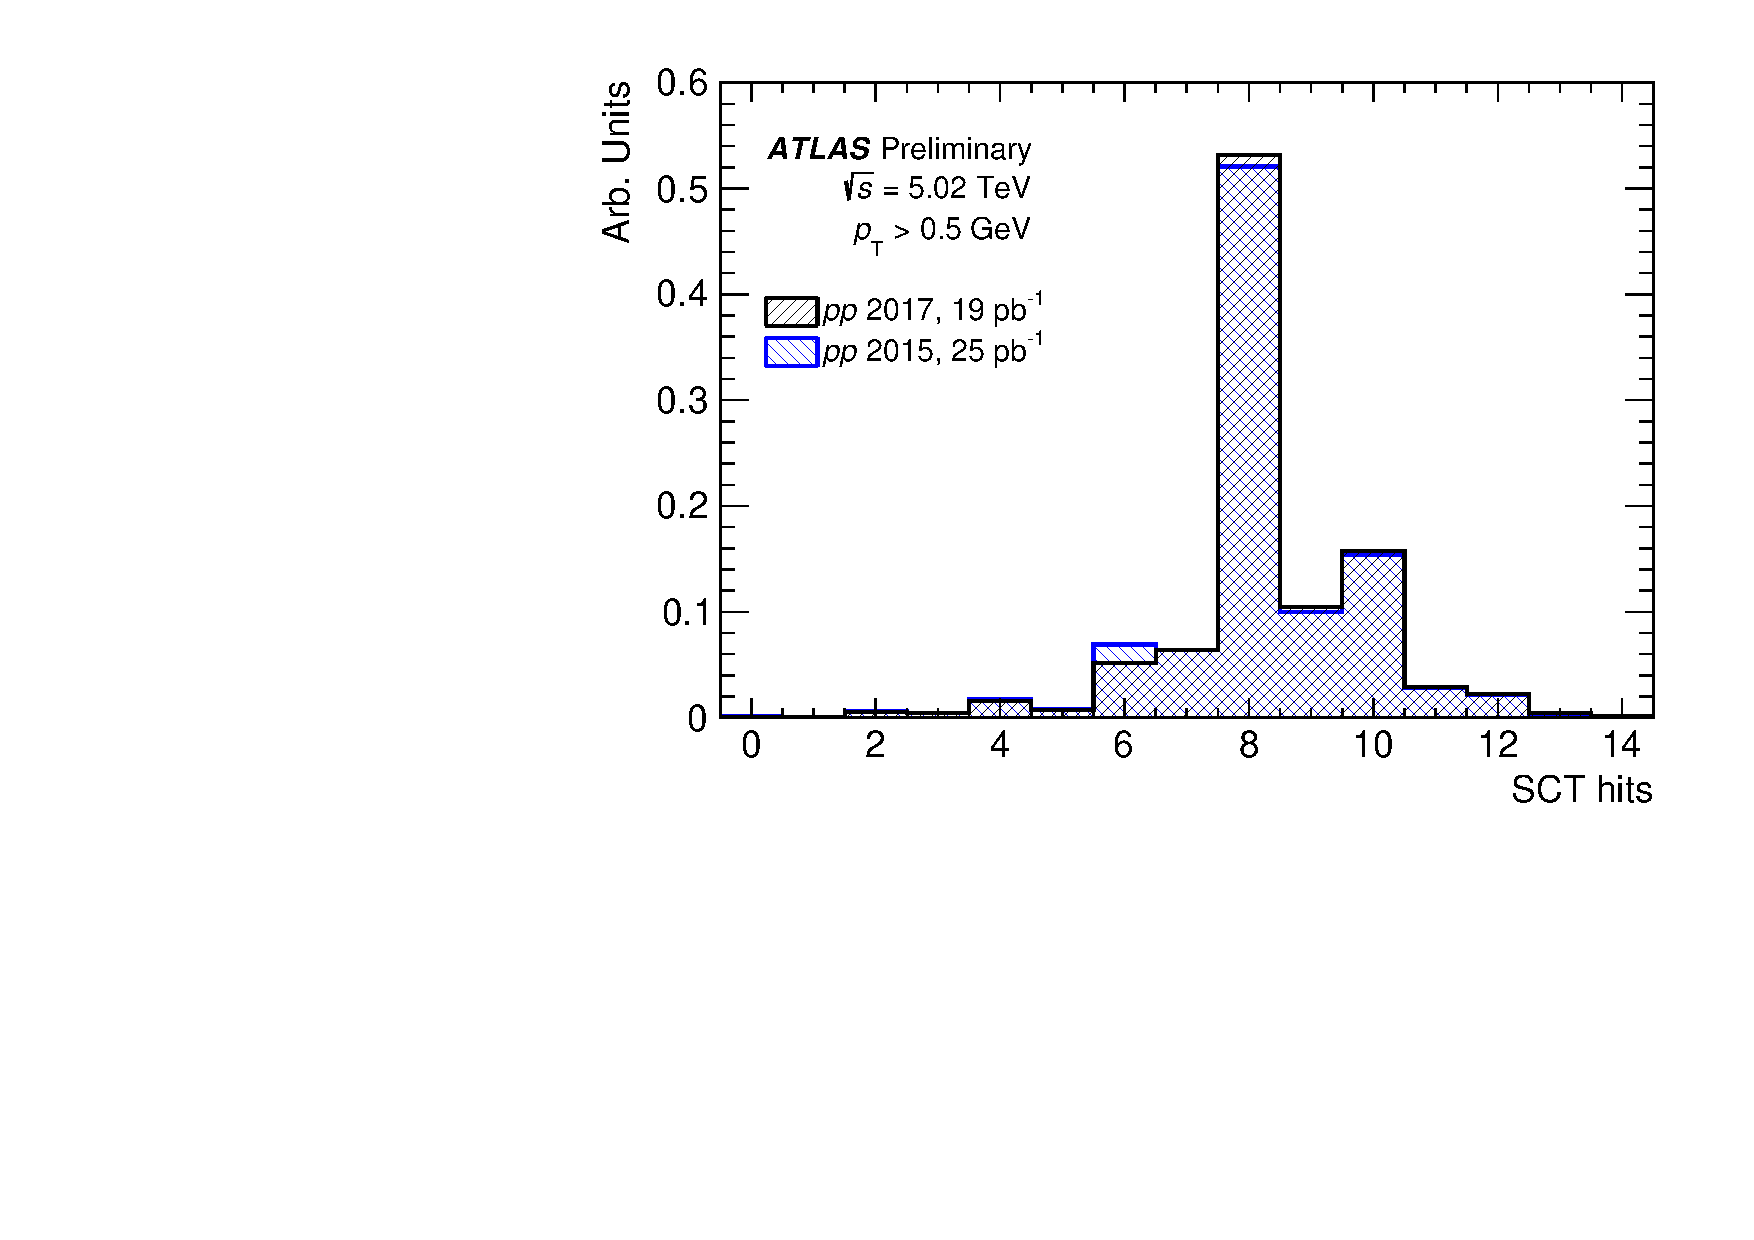
\includegraphics[width=.475\linewidth]{figs/chapter_detector/ATLAS_ID_SCT_hits2.pdf}
\caption{Left: an average number of SCT hits per track as a function of pseudorapidity. Right: a number of SCT hits per track. Tracks are required to have $\pT>0.5$ GeV. Events are required to have a reconstructed vertex.}
\label{fig:detector_ATLAS_ID_SCT_hits}
\end{figure}



\paragraph{TRT}

The Transition Radiation Tracker (TRT)~\cite{Abat:2008zza} consists of three parts: a barrel and two endcaps. Its basic elements are thin-walled proportional drift tubes, hereafter called straws. Straw tubes were chosen as detecting elements because they offer a high degree of modularity of the detector and because they can be easily integrated into a medium producing transition without compromising the continuous tracking concept. The barrel part is comprised of 52544 straws 144 cm in length oriented parallel to the beam. The two end-caps each contain 122880 straps 37 cm in length radially aligned to the beam axis. The detector geometry guarantees that particles cross 35-40 straws in a pseudorapidity interval from 0 to 2, providing continuous tracking at larger radii of the Inner Detector while enhancing its pattern recognition ability. The TRT was not used in the heavy-ion program due to high occupancy in most central events which limited its use for tracking and electron identification. The analyses presented here do not make use of the TRT hits information.



\subsubsection{Forward Calorimeter}

Calorimeters measure the energy a particle loses as it passes through the detector. It is usually designed to stop entire or absorb most of the particles coming from a collision, forcing them to deposit all of their energy within the detector. Calorimeters typically consist of layers of passive or absorbing high-density material, for example lead, interleaved with layers of an active medium such as solid lead-glass or liquid argon. Electromagnetic calorimeters measure the energy of electrons and photons as they interact with the matter. Hadronic calorimeters sample the energy of hadrons as they interact with atomic nuclei. Calorimeters can stop most known particles except muons and neutrinos.

Complete calorimeter hermeticity is important for many physics studies at the LHC. In order to extend the pseudorapidity coverage up to 4.9 units, ATLAS uses a liquid argon Forward Calorimeter (FCal)~\cite{Artamonov:2008zz} integrated into the endcap cryostat. The ATLAS FCal covers the pseudorapidity range $3.1 < |\eta| < 4.9$. The main challenge in designing the FCal was to ensure that it would function reliably in the extremely hostile environment close to the LHC beams. In order to have some measurement of longitudinal shower environment, the FCal is divided into three sections, as shown in Figure~\ref{fig:detector_ATLAS_FCal}. In all three sections the construction is such that only radiation hard materials are used, and there are no adhesives used in the joints. All three modules use a novel electrode structure. This consists of copper tubes parallel to the beam axis, which contain electrode rods. In the FCal1 the electrode rods and the calorimeter matrix are copper. This serves to ensure a good thermal conductivity close the shower maximum, and avoids local heating, and perhaps boiling of the liquid argon. In order to have an extremely dense detector, the FCal2 and FCal3 modules have tungsten electrode rods, and the matrix consists of small sintered tungsten slugs. The liquid argon gap between the electrode rods, and the copper electrodes tubes is maintained by a spiral of radiation hard PEEK plastic in all three modules.

\begin{figure}[H]
\centering
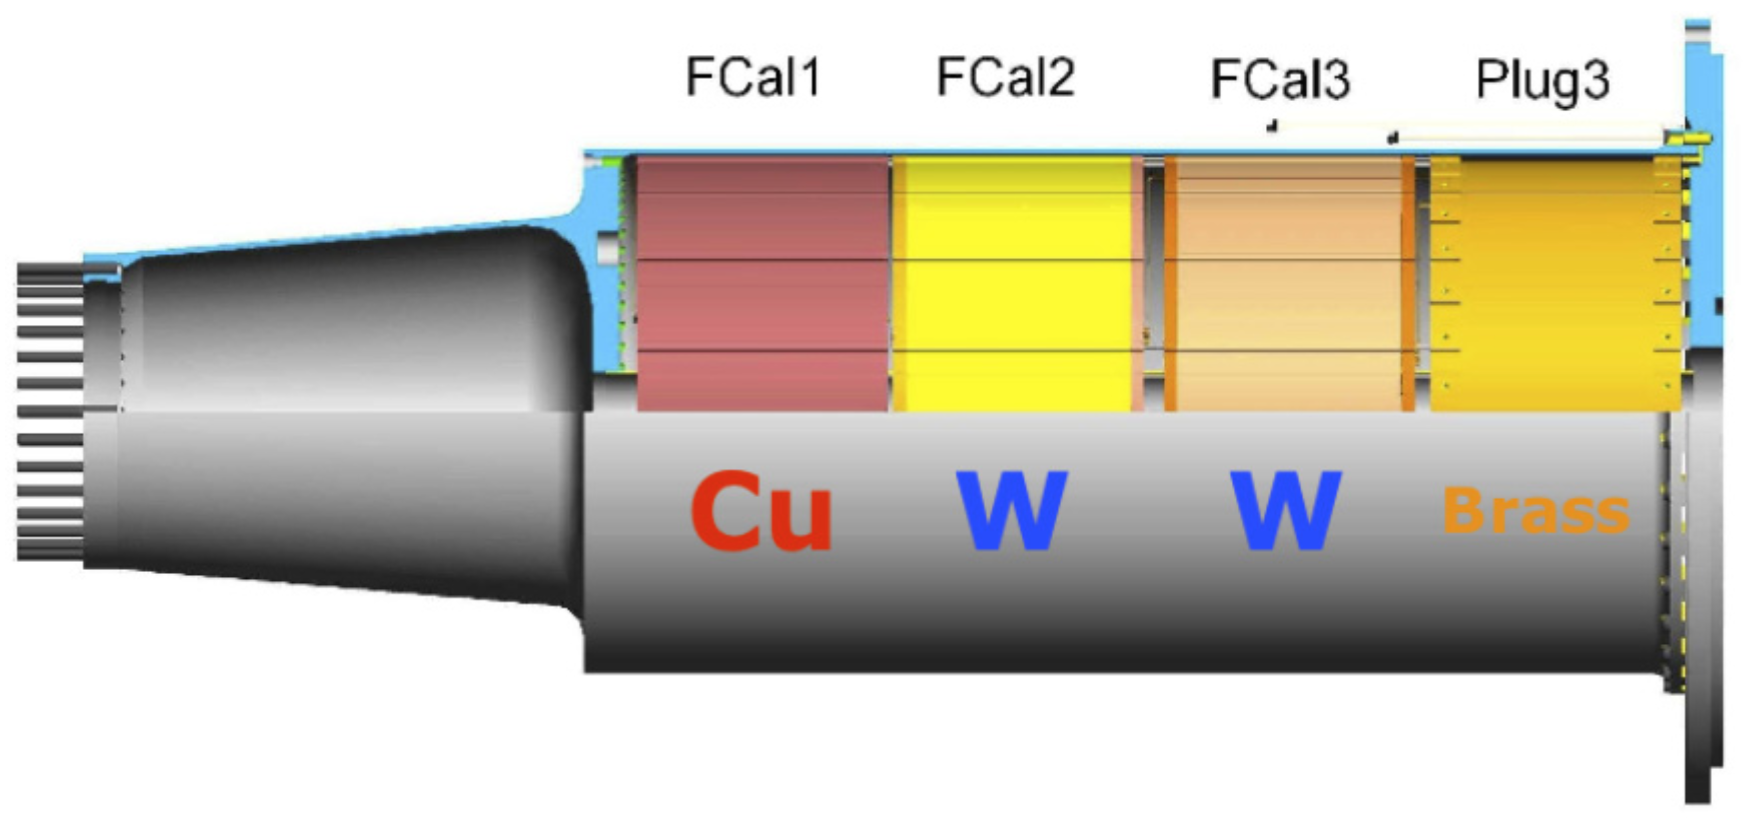
\includegraphics[width=.475\linewidth]{figs/chapter_detector/ATLAS_FCal.png}
\caption{The general arrangement of the FCal, and details of the electrode spacing.}
\label{fig:detector_ATLAS_FCal}
\end{figure}

Left panel of Figure~\ref{fig:detector_ATLAS_FCal_Nch} presents the correlation between number of reconstructed charged particles $\Nchrec$ and total transverse energy in FCal $\Et^\text{FCal}$. A strong correlation is observed. Since in most flow analysis azimuthal angular distribution is measured using charged particles, $\Et^\text{FCal}$ provides an independent observable to quantify the event activities. The determination of centrality using $\Et^\text{FCal}$ will be discussed in Section~\ref{sec:centrality_determination}.

\begin{figure}[H]
\centering
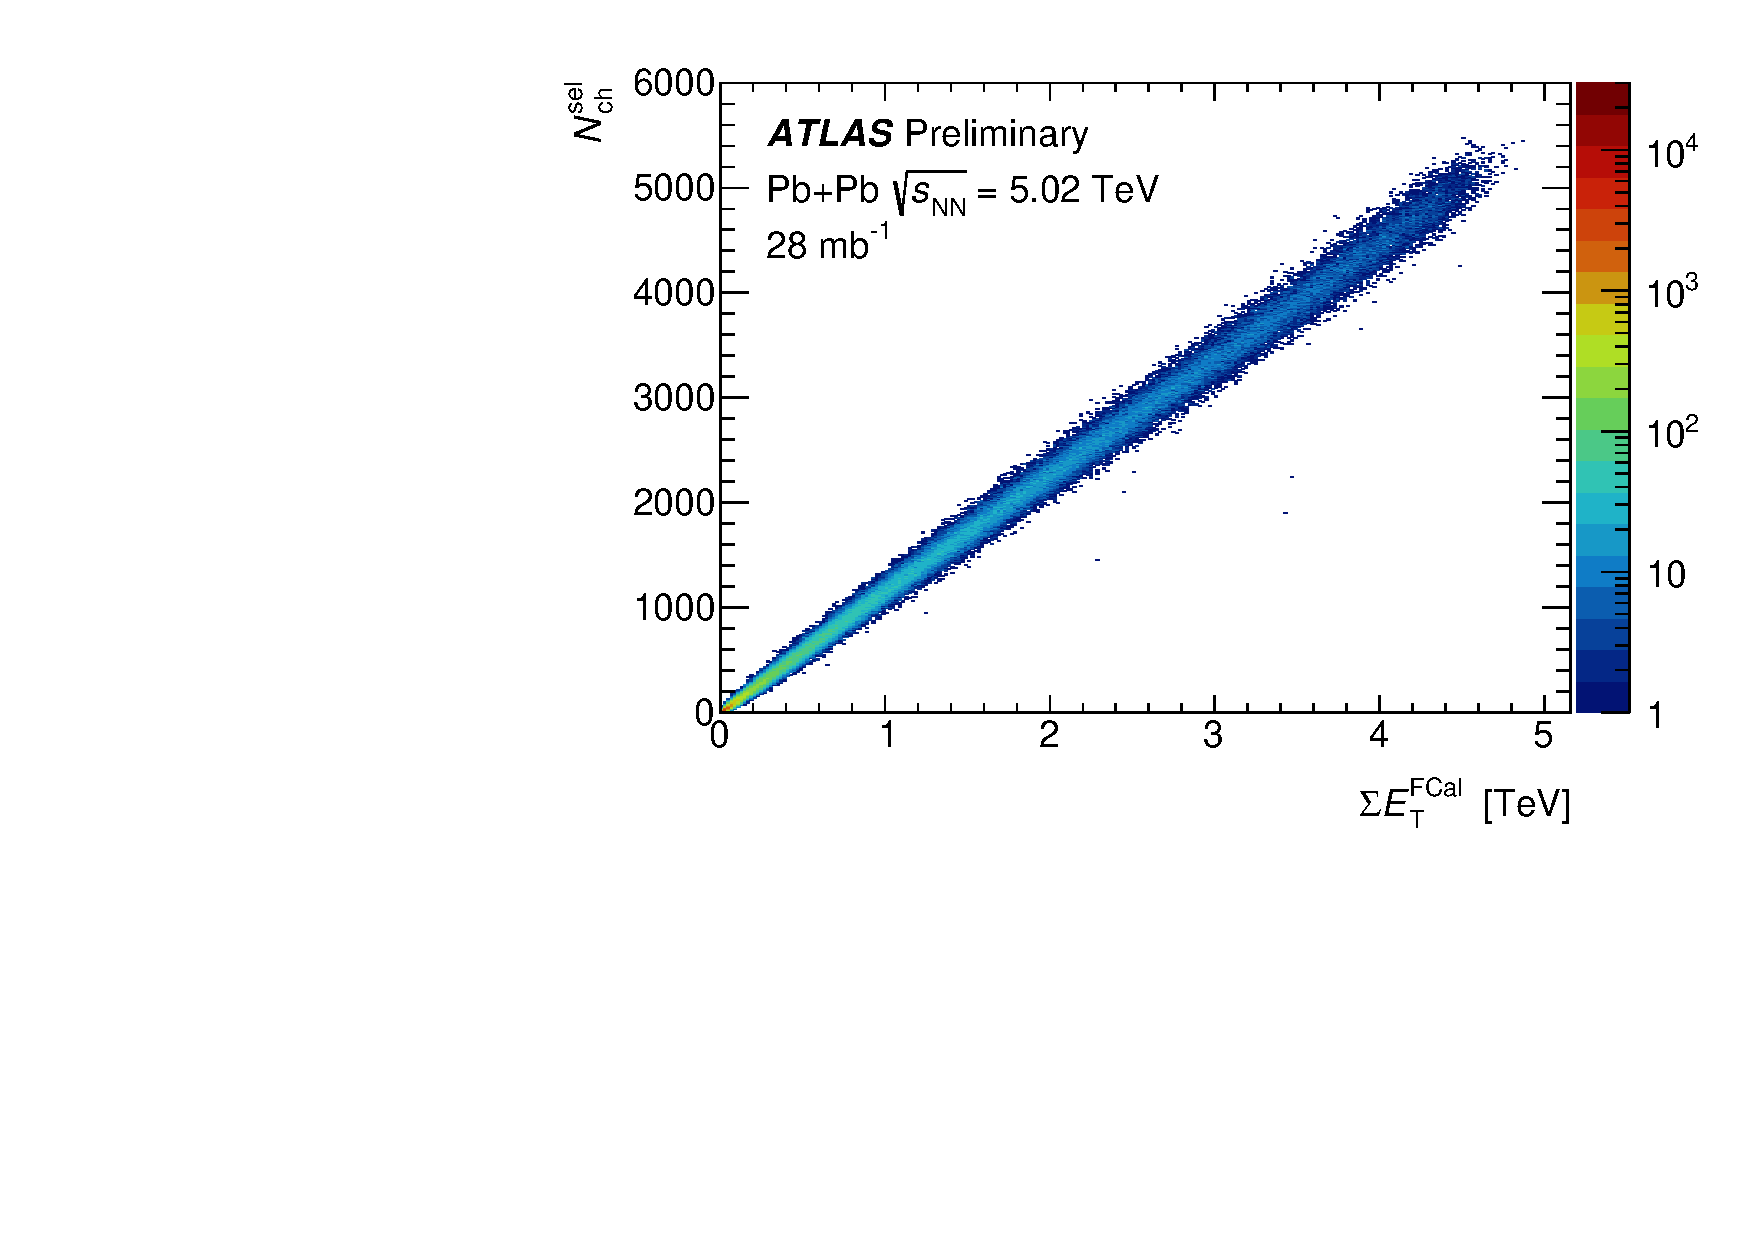
\includegraphics[width=.475\linewidth]{figs/chapter_detector/ATLAS_FCal_Nch.pdf}
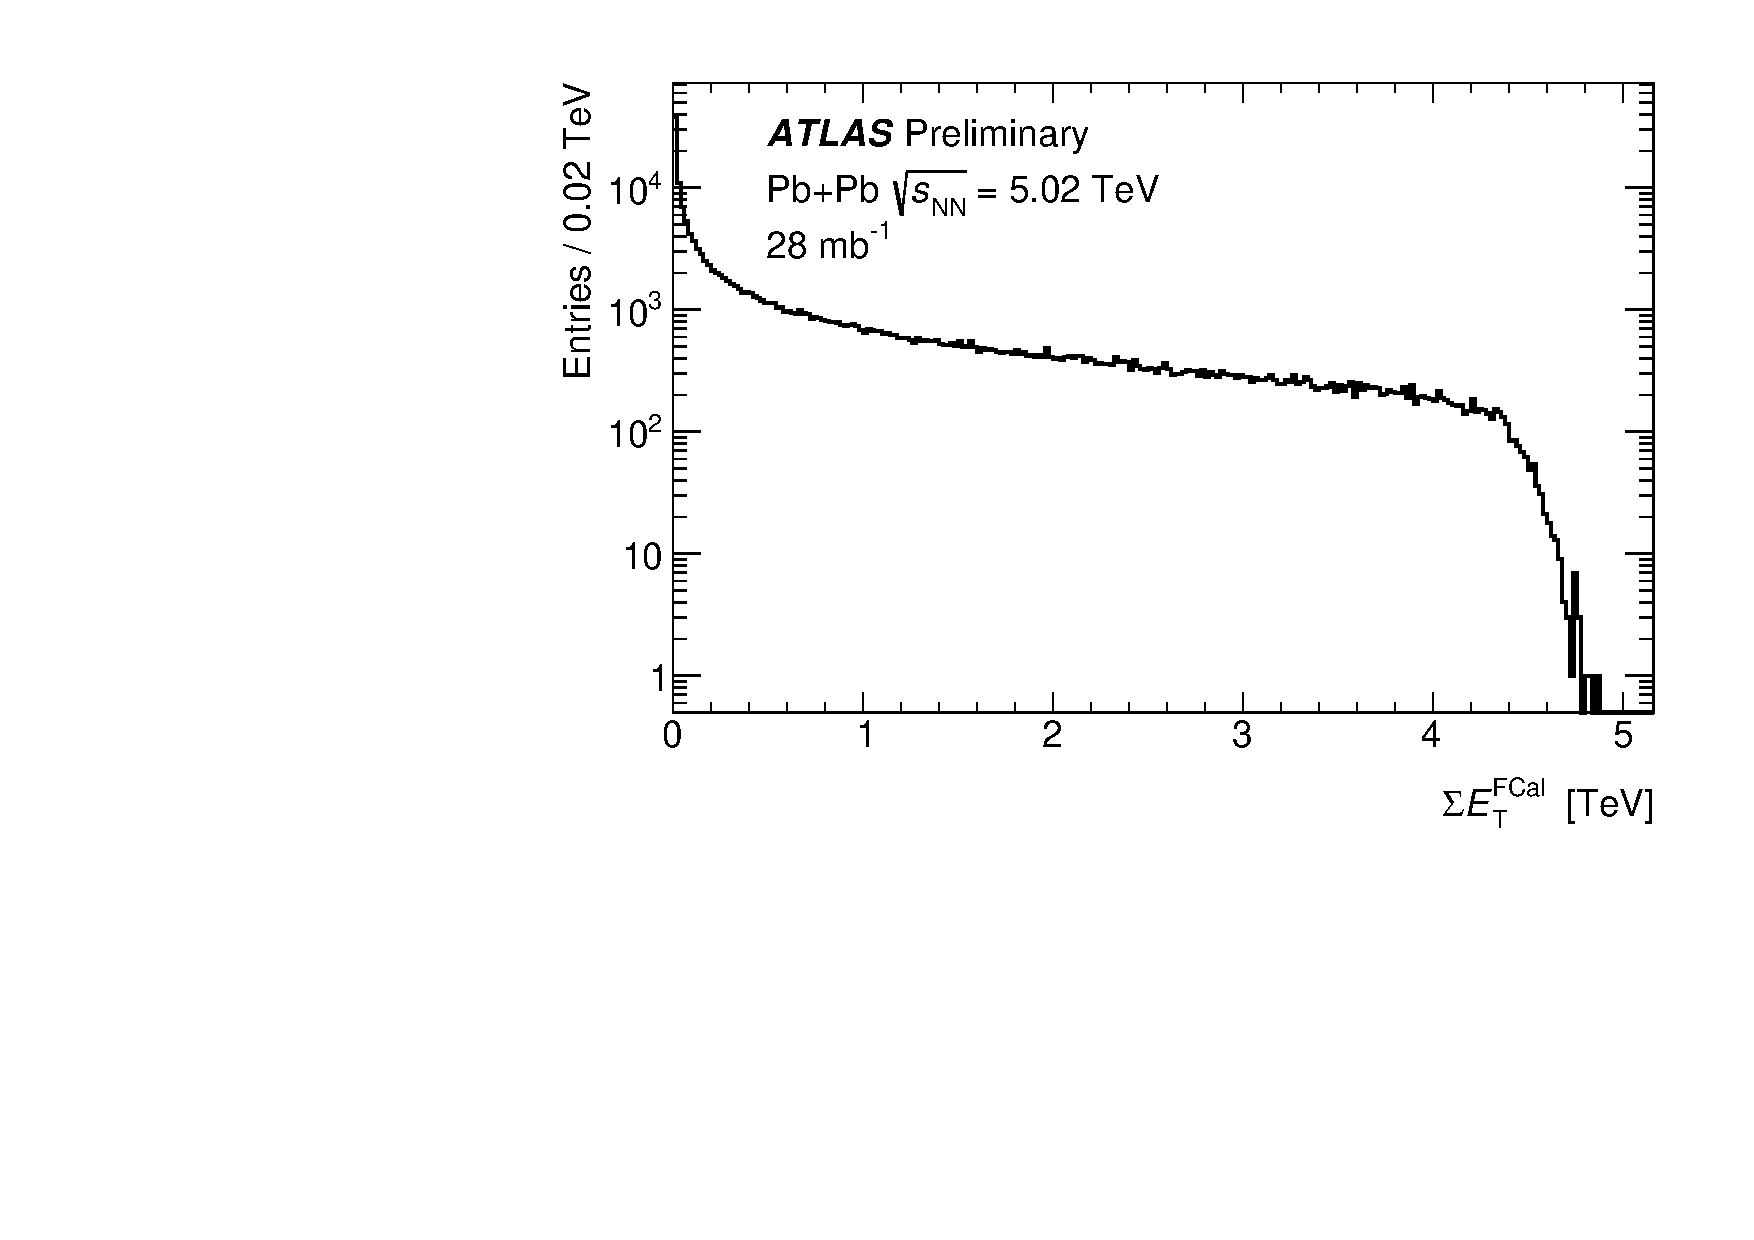
\includegraphics[width=.475\linewidth]{figs/chapter_detector/ATLAS_FCaldis.pdf}
\caption{Left: number of reconstructed charged particle $\Nchrec$, versus total transverse energy $\Et^\text{FCal}$ in the FCal. Tracks are selected from a pseudorapidity range $|\eta|<2.5$ with transverse momentum $\pT>0.3$ GeV. A reconstructed primary vertex is required. Right: distribution of $\Et^\text{FCal}$.}
\label{fig:detector_ATLAS_FCal_Nch}
\end{figure}



\subsubsection{Zero Degree Calorimeter}
\label{sec:zero_degree_calorimeter}

The primary role of Zero Degree Calorimeter (ZDC)~\cite{ATLAS:2007aa} is in event characterization. The ZDC measures the participant number by sampling the spectator neutrons. The ZDC can also measure the orientation of the impact parameter. The secondary role of the ZDC is as a device for luminosity measurement. The ZDC (coincidence) cross-section can be reliably calculated.

The ZDC is located 140 m from the centra of ATLAS on either side, after the beam-pipe splits into two, covering the region $|\eta|>8.3$. It gets its name as it is located along the beam (at zero degrees). Only the neutral particles from the event manage to reach the ZDC as the charged particles are deflected away by the magnetic fields in the beam-pipe. Thus in Pb+Pb collisions the ZDC measures spectator neutrons. Each side of the ZDC consists of four modules as shown in the left bottom panel of Figure~\ref{fig:detector_ATLAS_ZDC}. The detailed design of the modules is shown in the right panel of Figure~\ref{fig:detector_ATLAS_ZDC}. Each module consists of 11 tungsten plates 10 mm thick in the beam direction and steel plates at the front and back (also 10 mm thick). Sandwiched between the plates are 1.5 mm diameter quartz rods that run vertically and are viewed by photomultiplier tubes (PMT) from above, via light-pipes. The quartz rods collect Cherenkov radiation from shower particles and guide them to the PMTs. Each PMT is read out by several channels of a Pre Processor Module (PPM), The PPMs are 64 channel, 40 MHz, 10 bit ADCs. The first two ZDC modules on the C side and the second module on the A side also have quartz rods arranged in an x-y grid along the beam-pipe. These can be used for position measurements of the showers. They were however not used in any of the analyses presented here. 

\begin{figure}[H]
\centering
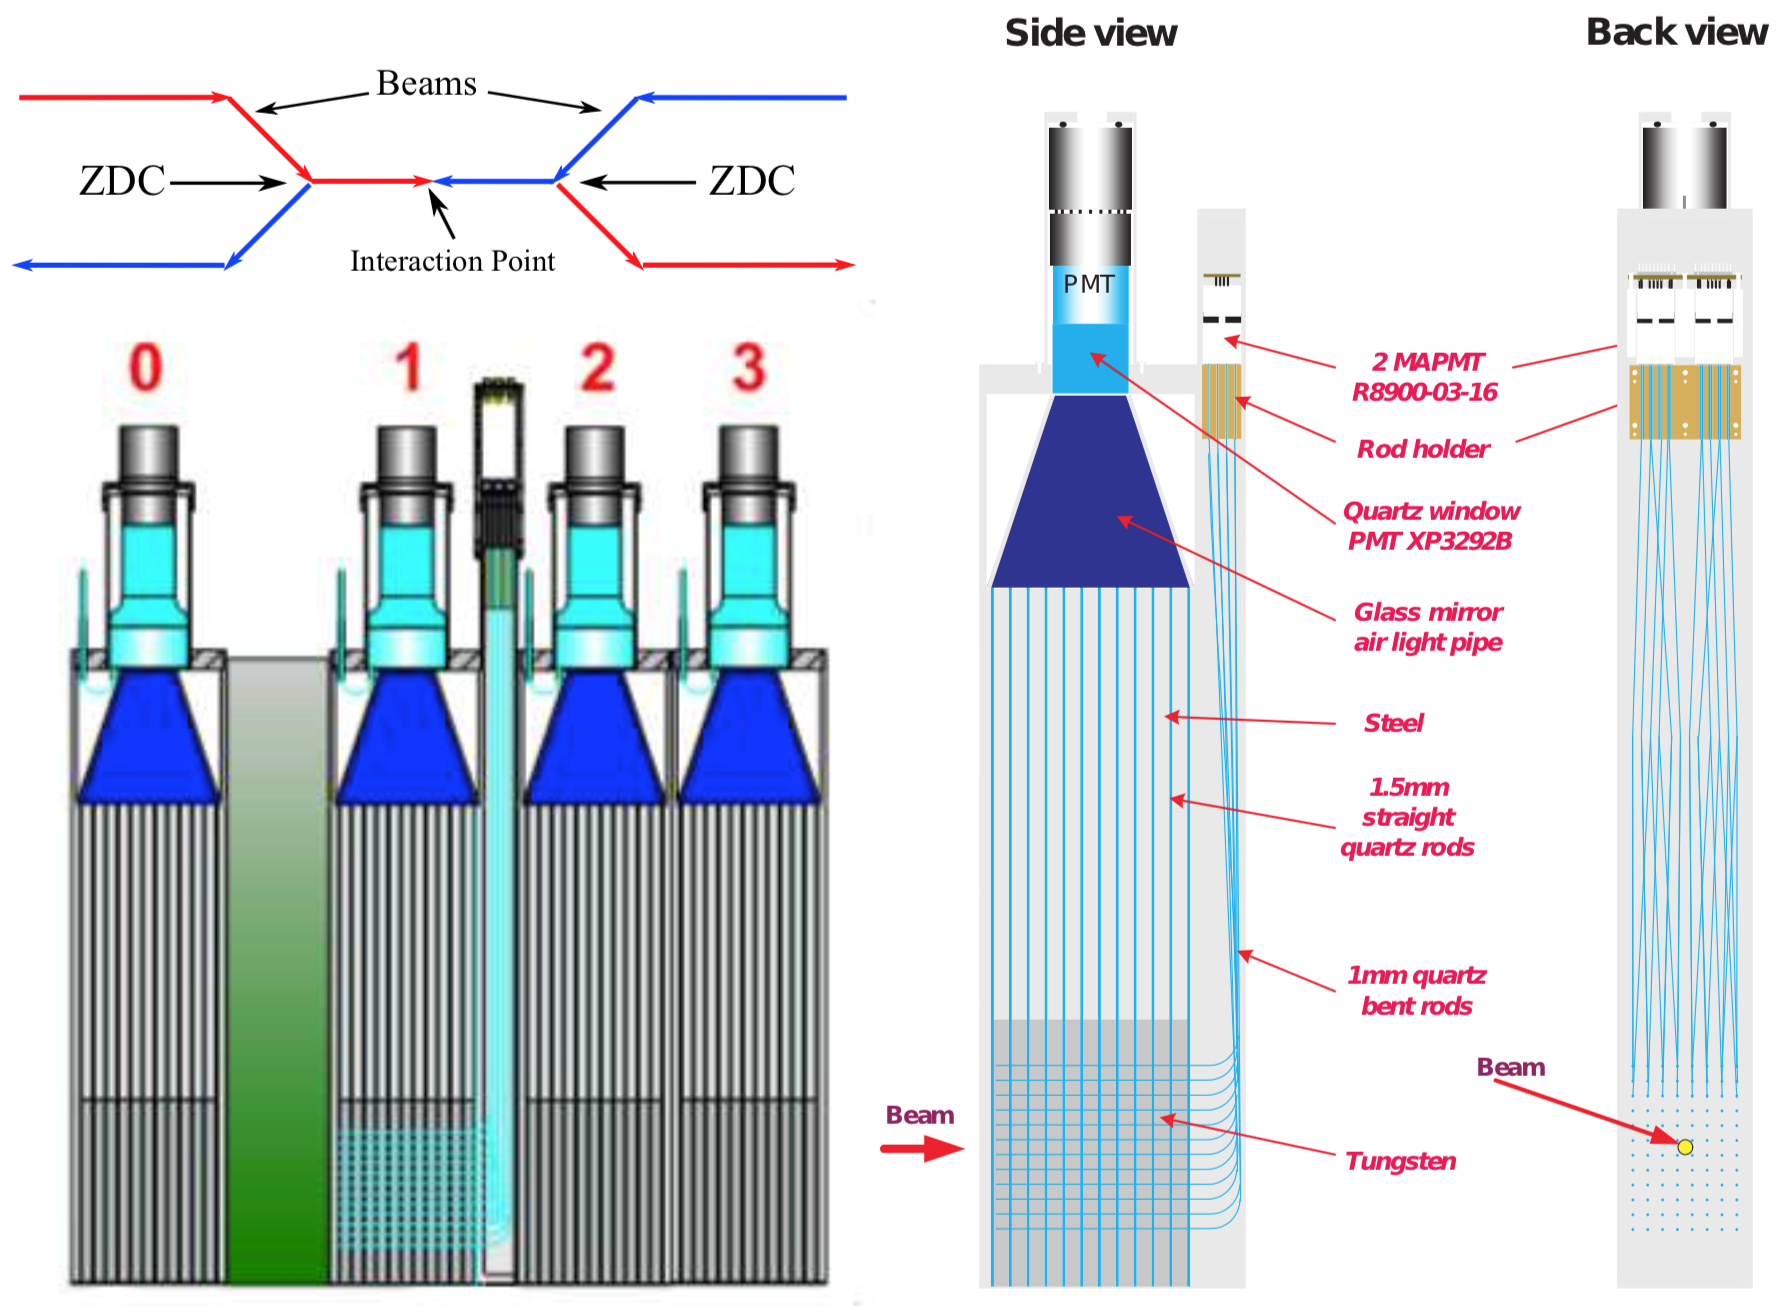
\includegraphics[width=.95\linewidth]{figs/chapter_detector/ATLAS_ZDC.png}
\caption{Left top: the location of the ZDC. Left bottom: the four ZDC modules on the A-side. Right: details of a ZDC module.}
\label{fig:detector_ATLAS_ZDC}
\end{figure}

To get an idea of the energy distribution deposited in ZDC, left panel of Figure~\ref{fig:detector_ATLAS_ZDC_FCal} shows the energy in the ZDC arm C, divided by the most probable energy of the single neutron peak. Peaks showing contributions from up to four neutrons emitted in a single event are clearly visible. Right panel of Figure~\ref{fig:detector_ATLAS_ZDC_FCal} shows the correlation of the sum of the energies in the two ZDC arms, normalized to the single neutron energy, v.s. the sum of transverse energies measured in the FCal. In peripheral collisions ($\Et^\text{FCal}<0.5$ TeV), sum of energies in ZDC and FCal are correlated. While from mid-central to central collisions ($\Et^\text{FCal}>1.0$ TeV), sum of energies in ZDC and FCal are anti-correlated. This is because in these collisions, ZDC mainly measures the energy from spectators, while FCal measures the energy from participants. Numbers of spectators and participants are anti-correlated. The additional events observed beyond the main band of the correlation are mostly pile-up events, i.e. events with more than one reconstructed vertices. This correlation can be used to suppress the fraction of pile-up events (Section~\ref{sec:event_selection}).

\begin{figure}[H]
\centering
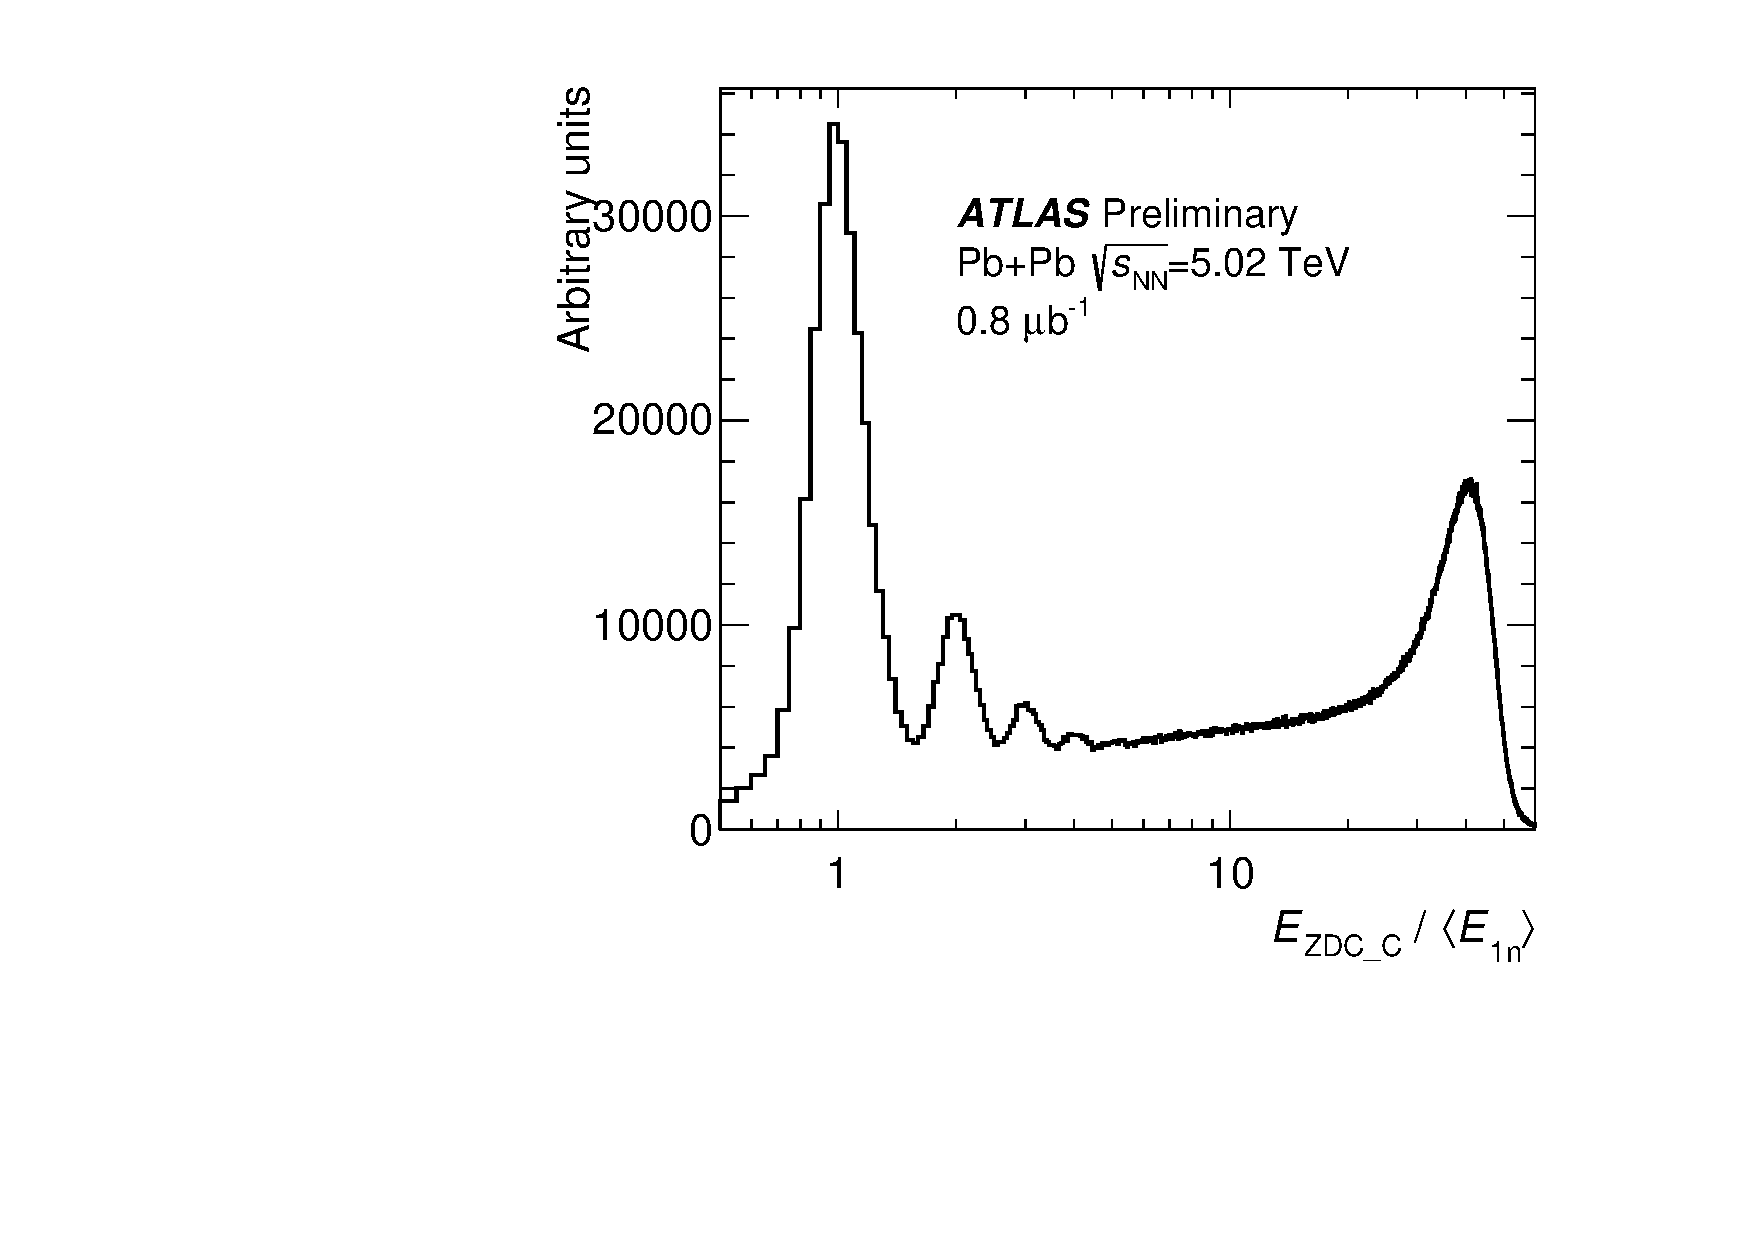
\includegraphics[width=.475\linewidth]{figs/chapter_detector/ATLAS_ZDCdis.pdf}
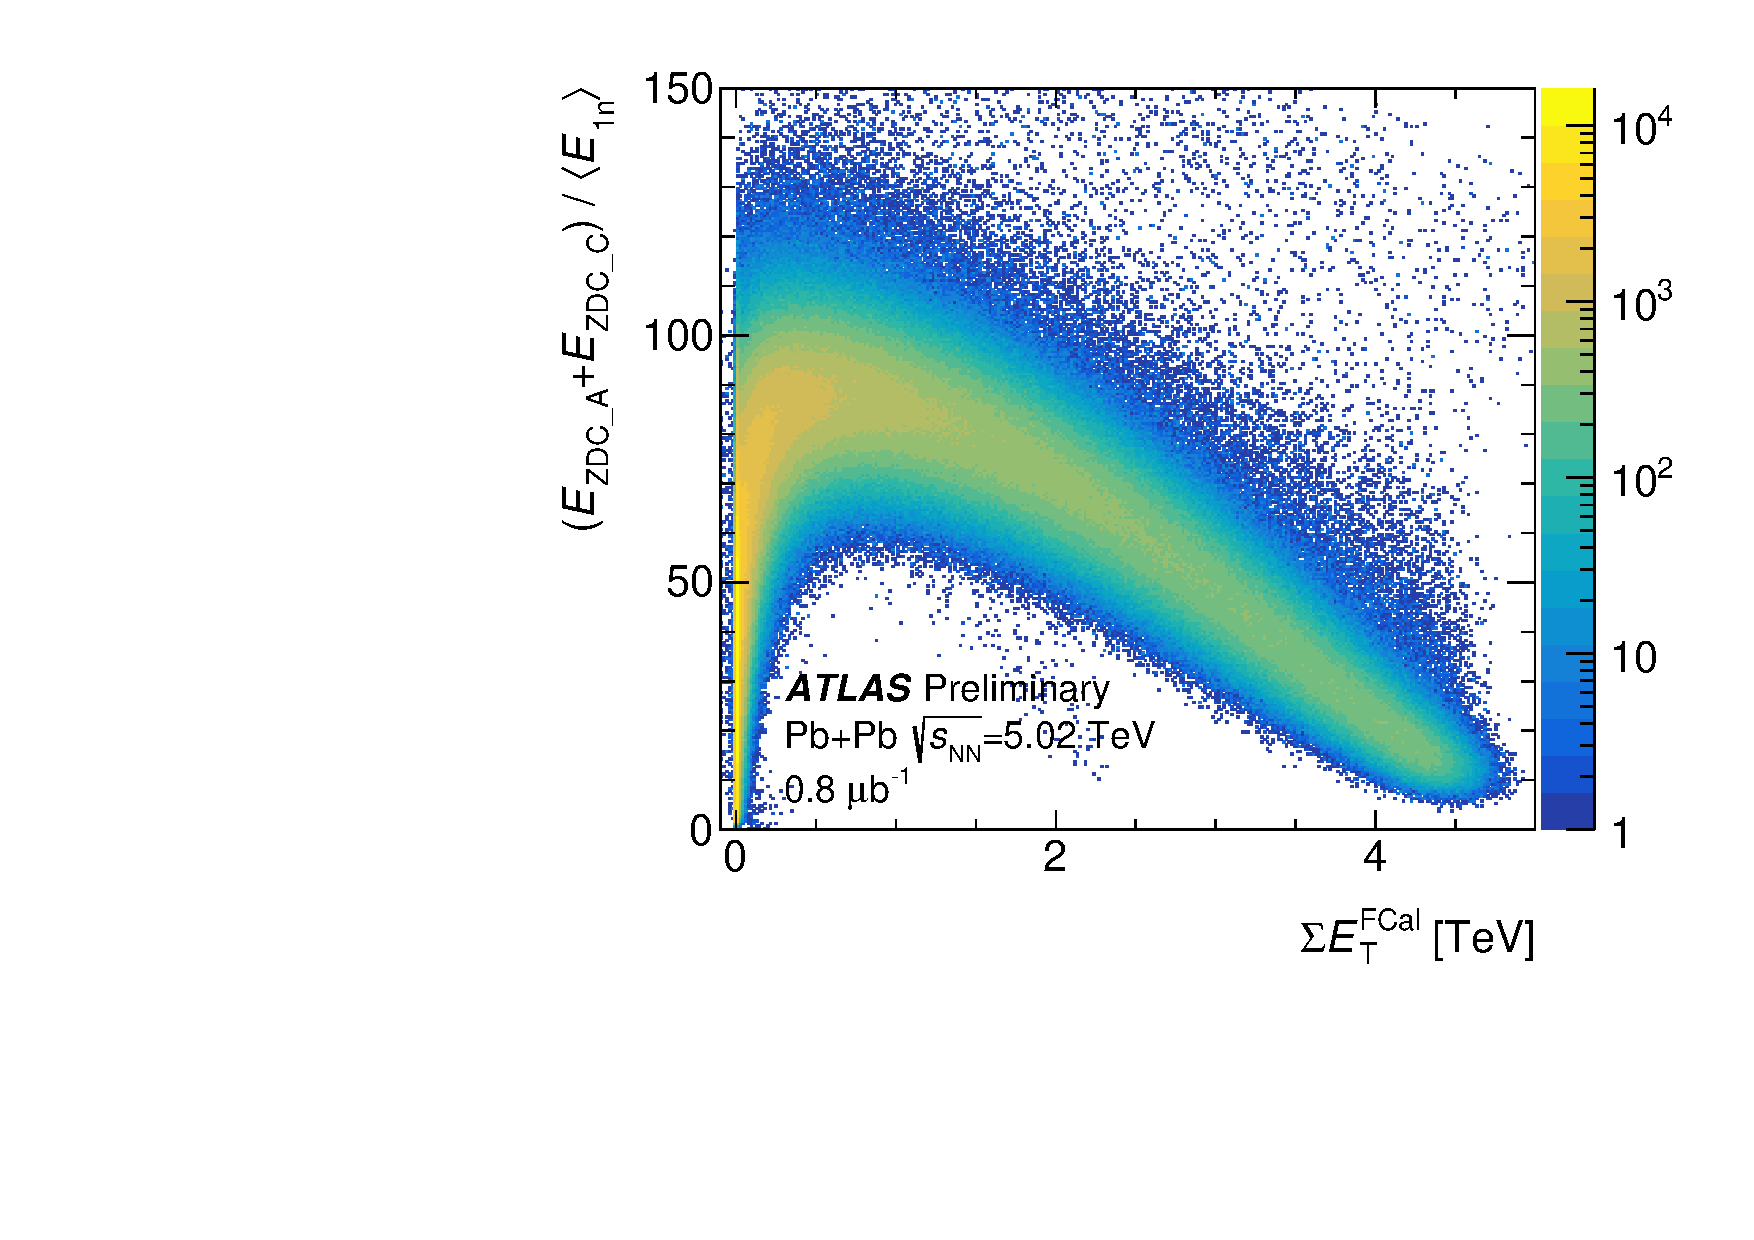
\includegraphics[width=.475\linewidth]{figs/chapter_detector/ATLAS_ZDC_FCal.pdf}
\caption{Left: Energy in the ZDC arm C (negative rapidity), divided by the most probable energy of the single neutron peak. Peaks showing contributions from up to four neutrons emitted in a single event are clearly visible. Right: Correlation of the sum of the energies in the two ZDC arms, normalized to the single neutron energy, v.s. the sum of transverse energies measured in the FCal. For both plots, a reconstructed vertex is also required to be present in each event.}
\label{fig:detector_ATLAS_ZDC_FCal}
\end{figure}



\subsubsection{Minimum-Bias Trigger Scintillators}

Minimum Bias Trigger Scintillators (MBTS)~\cite{Sidoti:2014kra} delivered the primary triggers for selecting events from real LHC collisions with the smallest bias. The MBTS consist of 2 cm thick polystyrene scintillator disks mounted on both sides of the interaction point at a distance of approximately 3.6 m along the beam pipe. Each side has an inner and outer ring in $\eta$ of eight counters in the azimuthal angle $\phi$, as shown in Figure~\ref{fig:detector_ATLAS_MBTS}. The outer counters pseudorapidity acceptance is $2.08 < |\eta| < 2.78$, while the acceptance for inner counters is $2.78 < |\eta| < 3.75$. Wavelength shifting fibers are embedded in grooves at the edges of the counters and are grouped at the center of the module between the two pieces of scintillator. These optical fibers guide the emitted light to PMTs. The MBTS signals, after being shaped and amplified in such a way that the pulse amplitude is proportional to the amount of energy deposited in the counter, are fed into leading edge discriminators and sent as 25 ns pulses to the Central Trigger Processor (CTP). The total charge collected as well as the arrival time of the signal are recorded. An MBTS hit is defined as a signal above the discriminator threshold. At the CTP input, the 32 MBTS signals are stretched to 200 ns and the hit multiplicity is calculated for each side independently. The CTP combines individual signals in L1 trigger items like $\verb|L1_MBTS_1|$, which require at least one hit in the MBTS detectors. The use of MBTS as minimum-bias triggers will be discussed in the data acquisition section.

\begin{figure}[H]
\centering
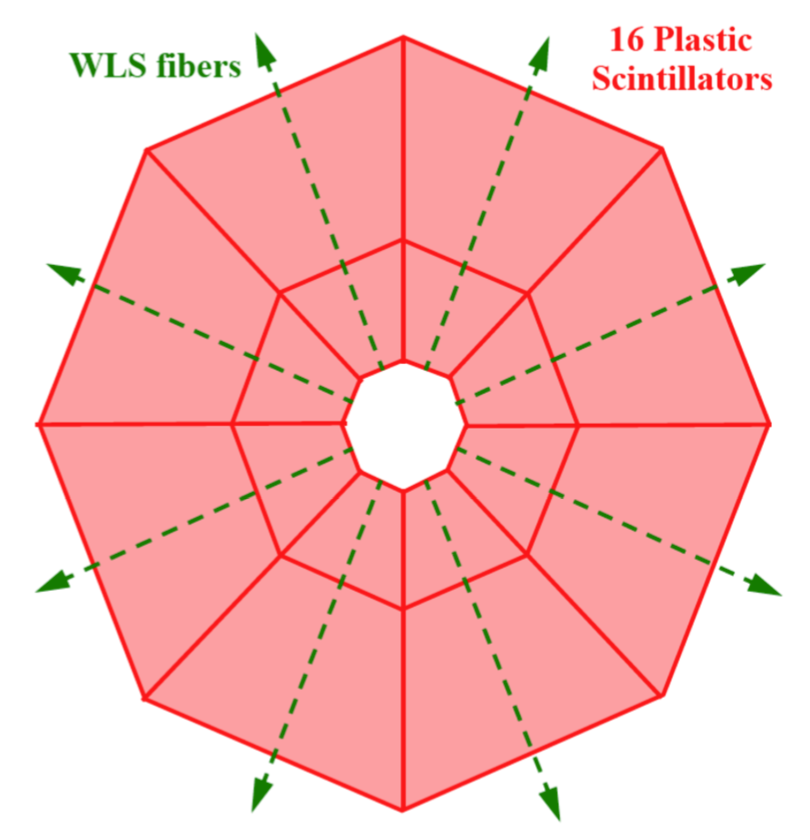
\includegraphics[width=.475\linewidth]{figs/chapter_detector/ATLAS_MBTS.png}
\caption{Layout of one of the two MBTS disks.}
\label{fig:detector_ATLAS_MBTS}
\end{figure}



\subsection{Data acquisition and selection}

The measurements presented in this thesis were gathered from the following data sets:
\begin{itemize}
\item Pb+Pb at $\sqrt{s_\text{NN}}=5.02$ TeV, recorded in 2015;
\item Xe+Xe at $\sqrt{s_\text{NN}}=5.44$ TeV, recorded in 2017;
\item $p$+Pb at $\sqrt{s}=5.02$ TeV, recorded in 2016;
\item $pp$ at $\sqrt{s}=13$ TeV, recorded in 2015 and 2016;
\end{itemize}
In the following sections, we will discuss the trigger, event selection, track selection and tracking efficiency, for each of the datasets above.



\subsubsection{Pb+Pb at $\sqrt{s_\text{NN}}=5.02$ TeV}

The Pb+Pb datasets were obtained from a sample of minimum-bias and ultra-central Pb+Pb collisions at $\sqrt{s_\text{NN}}=5.02$ TeV recorded by ATLAS in 2015 (Run 2). The corresponding integrated luminosity are approximately 470 $\mu b^{-1}$. The measurements were performed using the ATLAS inner detector and forward calorimeters.



\paragraph{Trigger}

The minimum-bias triggers for 5.02 TeV Pb+Pb collisions are:
\begin{itemize}
\item \verb|HLT_mb_sptrk_ion_L1ZDC_A_C_VTE50|
\item \verb|HLT_noalg_mb_L1TE50|
\end{itemize}
where \verb|sptrk| requires at least one reconstructed track at the HLT level, \verb|L1ZDC_A_C| requires at least one hit in both sides of ZDC detector. The major difference between these two triggers is Level-1 (L1) total energy \verb|TE|: \verb|VTE50| requires total energy less than 50 GeV while \verb|TE50| larger than 50 GeV.

To enhance the statistics in ultra-central collisions, Ultra-Central Collision (UCC) triggers are also included:
\begin{itemize}
\item \verb|HLT_hi_th1_ucc_L1TE14000|
\item \verb|HLT_hi_th2_ucc_L1TE14000|
\item \verb|HLT_hi_th3_ucc_L1TE14000|
\end{itemize}
where \verb|L1TE| denotes the minimum L1 total energy cut and \verb|th| corresponds to the various online minimum FCal Calorimeter $\Et$ cut at the High-Level Trigger (HLT) level.

Figure~\ref{fig:detector_ATLAS_trigger_PbPb502} shows the FCal $\Et$ distributions seeded by two major UCC triggers, compared with those seeded by minimum-bias (MinBias) triggers. UCC triggers collected about 20 times more event statistics compared with MinBias trigger in the ultra-central collisions. Furthermore, the turn-on curves of UCC trigger efficiencies are very shape, which means the selection bias caused by these triggers is negligible. The impact from trigger efficiency will be discussed in details in Section~\ref{sec:trigger_selection_bias}.

\begin{figure}[H]
\centering
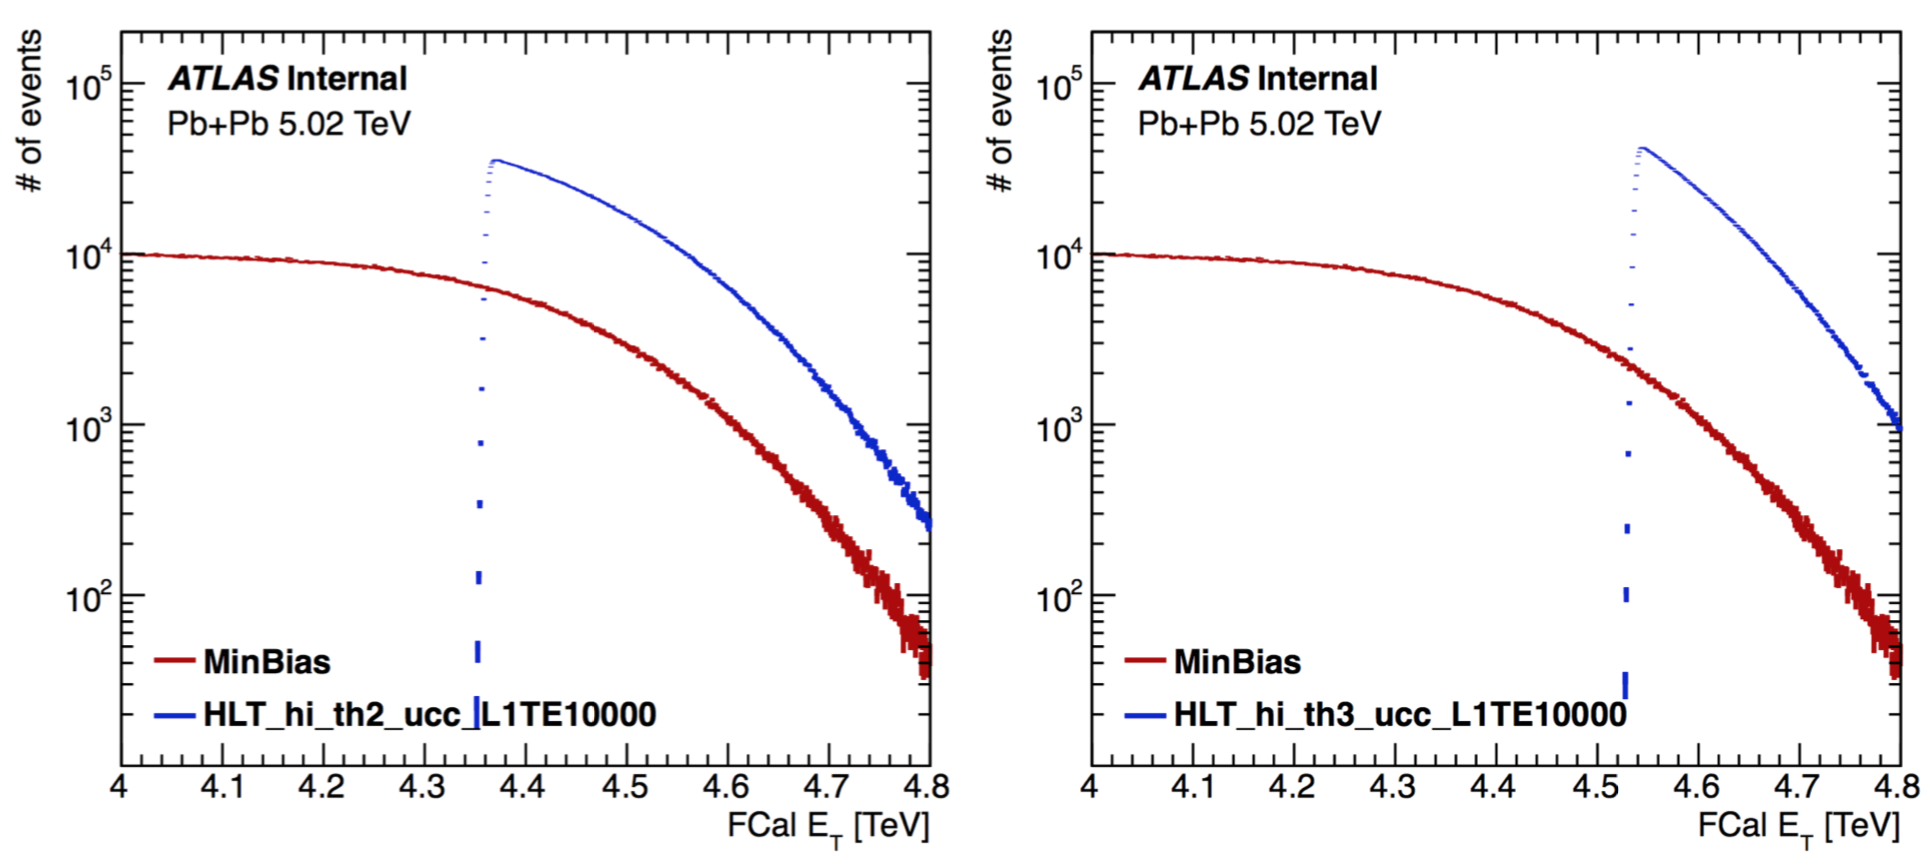
\includegraphics[width=.95\linewidth]{figs/chapter_detector/ATLAS_trigger_PbPb502.png}
\caption{FCal $\Et$ distributions for two major UCC triggers (red points), compared with MinBias trigger (blue points).}
\label{fig:detector_ATLAS_trigger_PbPb502}
\end{figure}



\paragraph{Event selection}
\label{sec:event_selection}

The event selections for 5.02 TeV Pb+Pb events are:
\begin{itemize}
\item Pass Good Run List (GRL);
\item Have a primary reconstructed vertex;
\item Events with detector errors (LAr, Tile, SCT) removed;
\item Vertex position cut: $|z_\text{vtx}|<100$ mm;
\end{itemize}
where the definitions of centrality and pileup events will be discussed below. In this thesis we are cutting the vertex position at 100 mm instead of 150 mm in previous published Pb+Pb analysis. This is because multiplicity distribution along $\eta$ changes with $z_\text{vtx}$ position, which might have a minor impact on forward-backward analysis and subevent cumulant analysis, since those analyses are highly $\eta-$dependent. In order to avoid introducing large multiplicity fluctuations in the forward $\eta$ region, we further constrain the vertex position to 100 mm, and we will not loose much statistics with this tighter cut.

In the 2015 Pb+Pb run, the luminosity conditions provided by the LHC result in an average probability of $0.1\%$ that an event contains two or more Pb+Pb collisions (pileup). The pileup events are suppressed by only using the tracks from primary vertex. The remaining pileup events are further suppressed on the correlation between energies deposited in FCal and ZDC. This signal in the ZDC is calibrated to the number of detected neutrons $N_n$ based on the location of the peak corresponding to a single neutron. Figure~\ref{fig:detector_ATLAS_pileup_PbPb502} shows the procedure of pileup rejection and its performance. The left panel shows the correlation between number of neutrons in the ZDC and total transverse energy $\Et$ in the FCal. The ``banana''-shaped main band covers the events with a single vertex. While in a pileup event, both the number of neutrons and FCal $\Et$ are larger than those from a single event, and this is illustrated by the events in the ``grass'' region above the main band. To clean up the pileup, one way is by applying a linear cut on the correlation map, indicated by the black straight line, and another approach is cutting off $0.1\%$ of the events in the tails of $N_\text{neutrons}$ distribution in each FCal $E_\text{T}$ slice, indicated by the red curve. In this analysis, we will use the $0.1\%$ cut as the default cut. The right panel shows the performance of the two pileup rejection methods just mentioned. The Y-axis represents the fraction of rejected pileup events out of all the pileup events. The rejection rate is low at low FCal $\Et$, this is because the band for pileup events mostly overlaps with the main band for single events. However, since the fraction of pileup events is very low in peripheral collisions, the low rejection rate has no impact on the results. On the other hand, the rejection rate reaches $100\%$ in UCC, where the fraction of pileup event is high, meaning that almost all the pileup events are rejected using this $0.1\%$ pileup cut. The systematics relating to the pileup cut will be discussed in Section~\ref{sec:pileup_rejection}.

\begin{figure}[H]
\centering
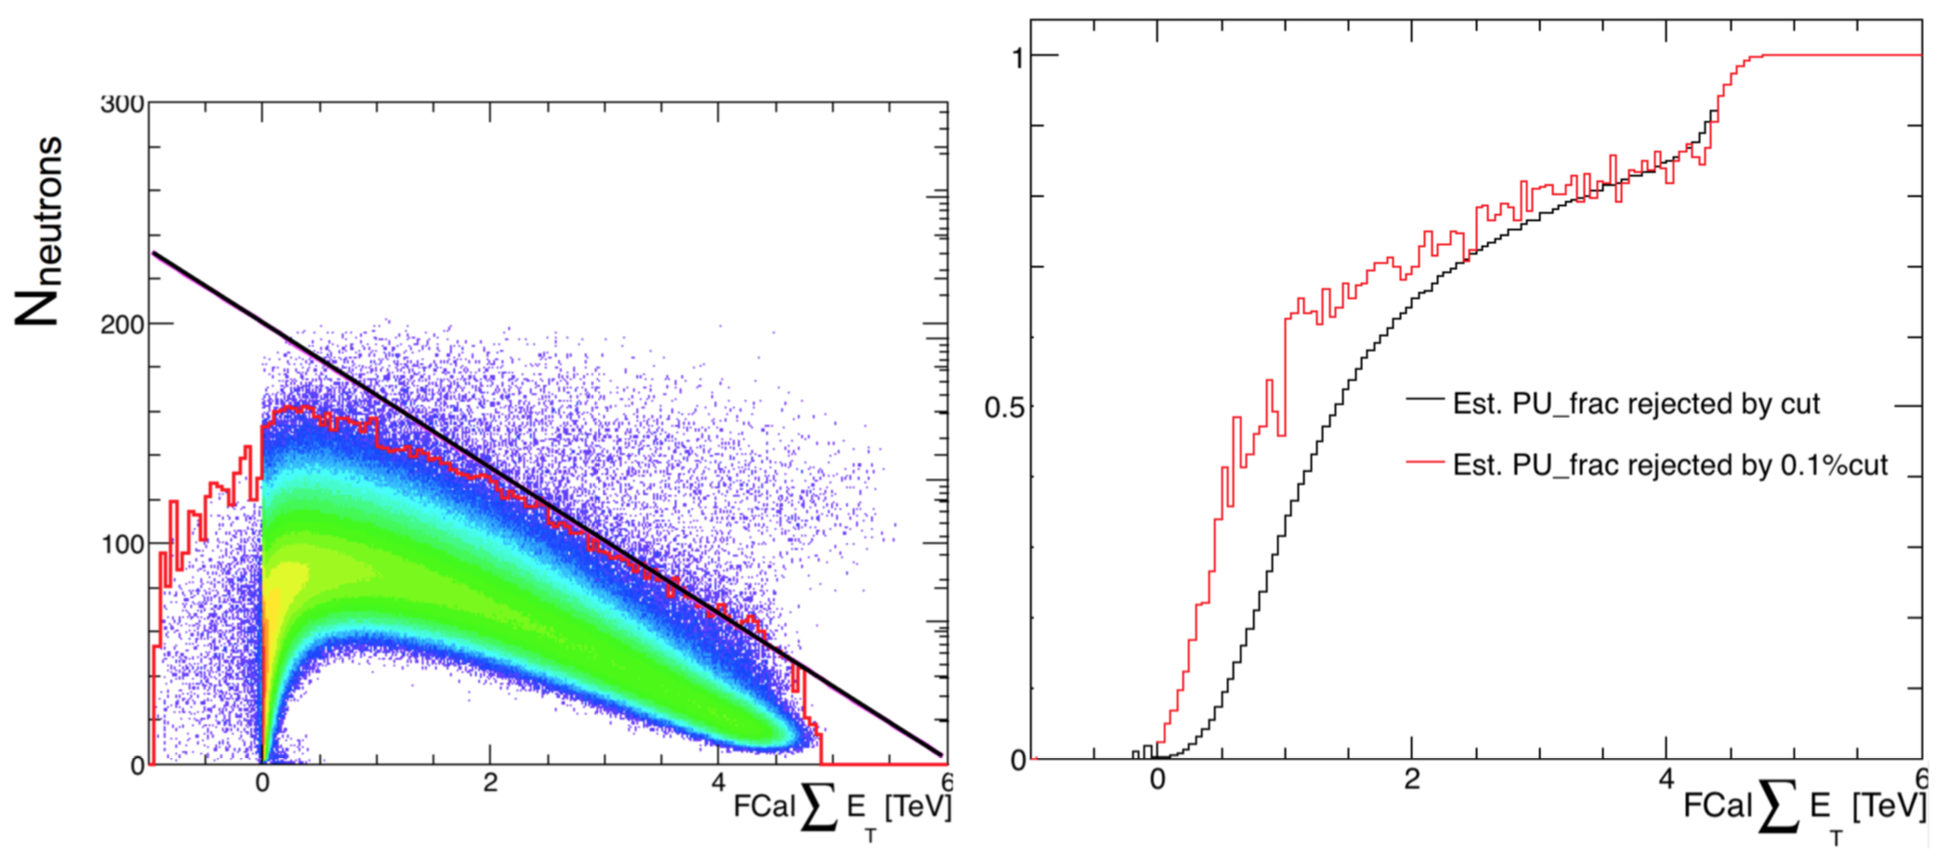
\includegraphics[width=.95\linewidth]{figs/chapter_detector/ATLAS_pileup_PbPb502.png}
\caption{Left: the correlation between calibrated number of neutrons in the ZDC and FCal $\Et$. Right: the fraction of rejected pileup events in all pileup events. Two rejection criteria are shown: a linear cut and $0.1\%$ cut.}
\label{fig:detector_ATLAS_pileup_PbPb502}
\end{figure}



\paragraph{Centrality determination}
\label{sec:centrality_determination}

The heavy-ion collision geometry is defined by its impact parameter $b$. As the actual event-by-event impact parameter is not accessible experimentally, the centrality classification is based on the transverse energy measured in the FCal, $\Et^\text{FCal}$, which exhibits a strong monotonic correlation with $b$. A model based on the Monte Carlo (MC) Glauber approach~\cite{Miller:2007ri} is used to obtain the mapping from the observed $\Et^\text{FCal}$ to the primary properties, such as the number of binary nucleon-nucleon interactions, $N_\text{coll}$, or the number of nucleons participating in the nuclear collision, $N_\text{part}$, for each centrality interval. The Glauber model also provides a correspondence between the $\Et^\text{FCal}$ distribution and the sampling fraction of the total inelastic Pb+Pb cross-section, allowing the setting of the centrality percentiles. For this analysis a selection of the $80\%$ most central collisions (i.e. centrality 0-80$\%$) is used to avoid any diffractive, photonuclear, and other inelastic process that contribute significantly to very peripheral collisions. Figure~\ref{fig:detector_ATLAS_centrality_PbPb276} shows the distribution of $\Et^\text{FCal}$ in the 2.76 TeV Pb+Pb data, and thresholds for the selection of several centrality intervals. Uncertainties of centrality determination are shown in Section~\ref{sec:centrality_definition}.

\begin{figure}[H]
\centering
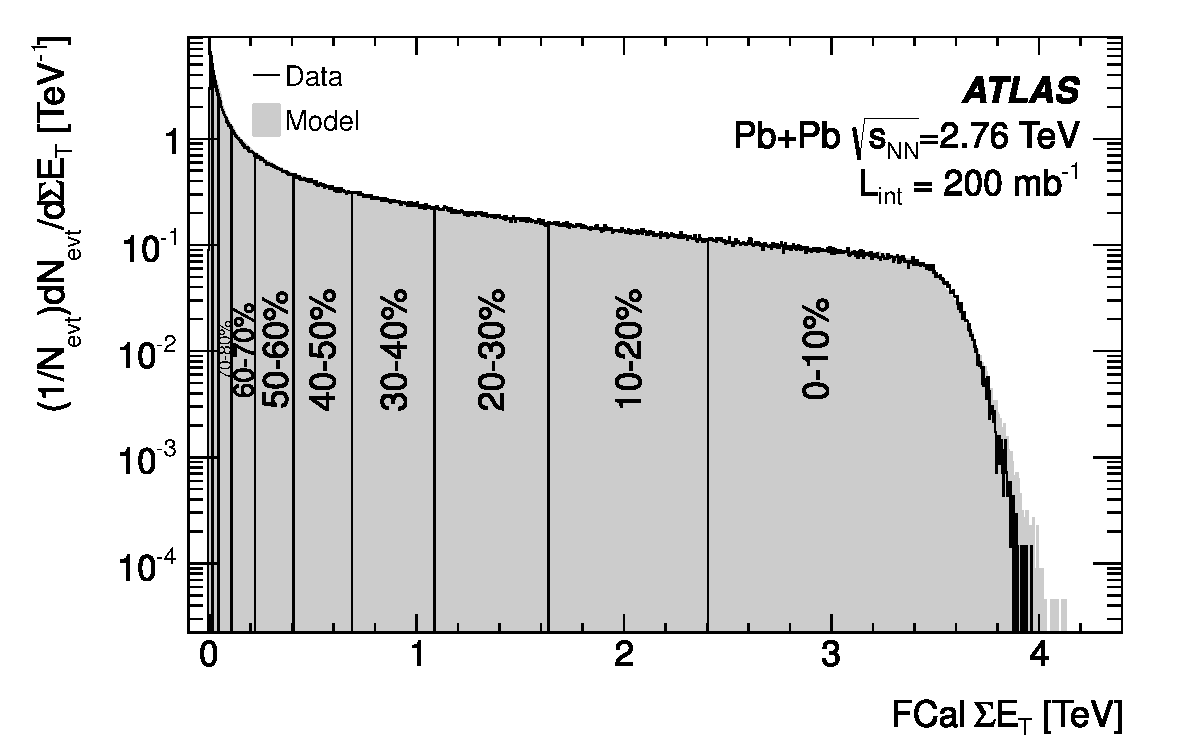
\includegraphics[width=.6\linewidth]{figs/chapter_detector/ATLAS_centrality_PbPb276.pdf}
\caption{Measured $\Et^\text{FCal}$ distribution divided into $10\%$ centrality intervals (black). This figure is taken from Ref.~\cite{ATLAS:2011ah}}
\label{fig:detector_ATLAS_centrality_PbPb276}
\end{figure}



\paragraph{Track selection, efficiency and fake rate}
\label{sec:track_selection_efficiency_and_fake_rate}

The default track selection for the Pb+Pb analysis is HILoose, which is defined as:
\begin{itemize}
\item number of pixel hits $> 0$;
\item number of SCT hits + dead sensors $\geq 6$;
\item if IBL hit is expected: at least 1 IBL hit required;
\item if no IBL hit is expected: a Layer-0 hit if expected;
\item $|d_0| \leq 1.5$ mm;
\item $|z_0 - z_\text{vtx}|\text{sin}\theta \leq 1.5$ mm;
\end{itemize}
where $d_0$ is the minimum transverse distance between a track and its associated vertex, and $z_0$ is the minimum longitudinal distance between a track and vertex. In Section~\ref{sec:track_selection}, a tighter cut, HITight, is applied to check the stability of tracking reconstruction.

To estimate the tracking efficiency and fake rate, HIJING MC samples with similar detector conditions are used. For the reconstructed tracks, the primary tracks, $N_\text{ch}^\text{primary}$, are defined as:
\begin{itemize}
\item pass the HILoose track quality selection;
\item truth match probability $>0.5$;
\item associated truth particle is a primary particle;
\end{itemize}
where truth match probability measures the probability of a reconstructed track matched to its truth track. The primary particle is defined at the truth level:
\begin{itemize}
\item status = 1, charge $!=$ 0;
\item 0 $<$ Barcode $<$ 2E5;
\item strange baryons are excluded;
\end{itemize}

The tracking efficiency $\epsilon$ can then be defined as:
\begin{equation}
\epsilon(\pT, \eta, \text{centrality}) \equiv \frac{N_\text{ch}^\text{primary}}{N_\text{ch}^\text{truth}},
\end{equation}
where $N_\text{ch}^\text{truth}$ denotes the number of primary particles at the truth level, all of which passed the HILoose track quality selection.

The tracking efficiency map is evaluated as a function of $\pT$, $\eta$ and centrality, and the results are shown in Figure~\ref{fig:detector_ATLAS_track_eff_PbPb502}, for different $\pT$ ranges and centralities. $\epsilon(\eta)$ is highest in mid-rapidity $-1<\eta<1$, and decrease by $20\%$ in forward-rapidity. As collision moves to peripheral, the efficiency increases. The tracking efficiency slightly increases towards higher $\pT$. Efficiency from HILoose is higher than HITight as expected.

\begin{figure}[H]
\centering
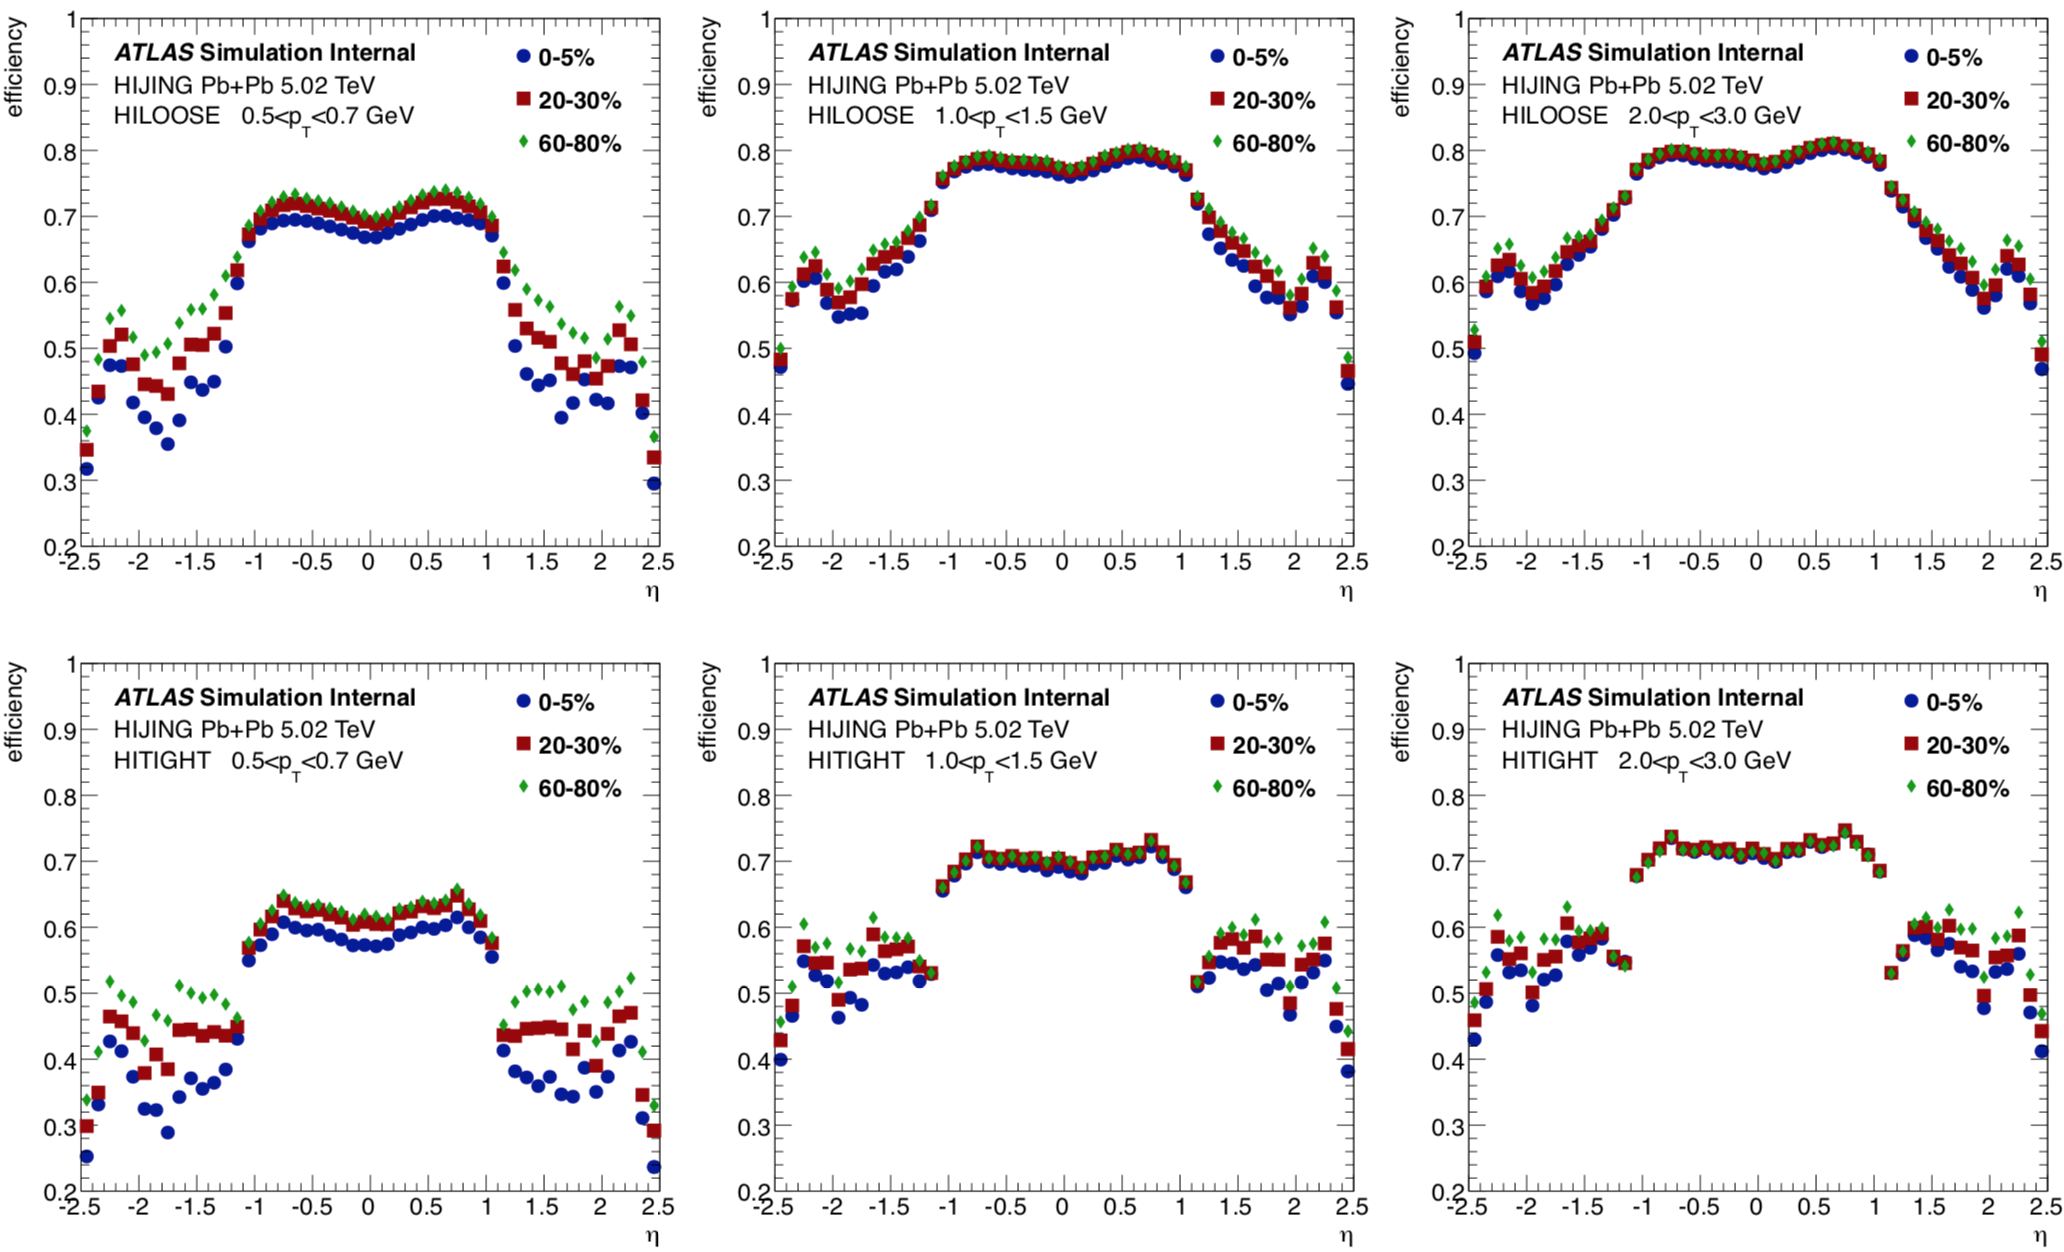
\includegraphics[width=.95\linewidth]{figs/chapter_detector/ATLAS_track_eff_PbPb502.png}
\caption{5.02 TeV Pb+Pb tracking efficiency $\epsilon(\eta)$, for different $\pT$ ranges and centralities. Top row is for HILoose and bottom row is for HITight.}
\label{fig:detector_ATLAS_track_eff_PbPb502}
\end{figure}

The fake track is defined as:
\begin{itemize}
\item pass the HILoose track quality selection;
\item fulfill one of the following:
\begin{itemize}
\item truth match probability $<0.5$;
\item not associate with truth particles;
\item Barcode = 0 of associated truth particle;
\end{itemize}
\end{itemize}

The faction of fake tracks (fake rate) $f$ is defined as:
\begin{equation}
f(\pT, \eta, \text{centrality}) \equiv \frac{N_\text{ch}^\text{fake}}{N_\text{ch}^\text{primary} + N_\text{ch}^\text{fake}},
\end{equation}
where $N_\text{ch}^\text{fake}$ denotes the number of fake tracks.

One of the focuses of our studies is on UCC collisions, where fake rate is significantly higher than MB events. The fake rates map is evaluated as a function of $\pT$, $\eta$ and centrality, and the results are shown in Figure~\ref{fig:detector_ATLAS_track_fake_PbPb502}. $f(\eta)$ is lowest in mid-rapidity $-1<\eta<1$, and increases by more than two times in forward-rapidity. As collision moves to peripheral, the fake rate significantly deceases. The fake rate decreases significantly towards higher $\pT$.

\begin{figure}[H]
\centering
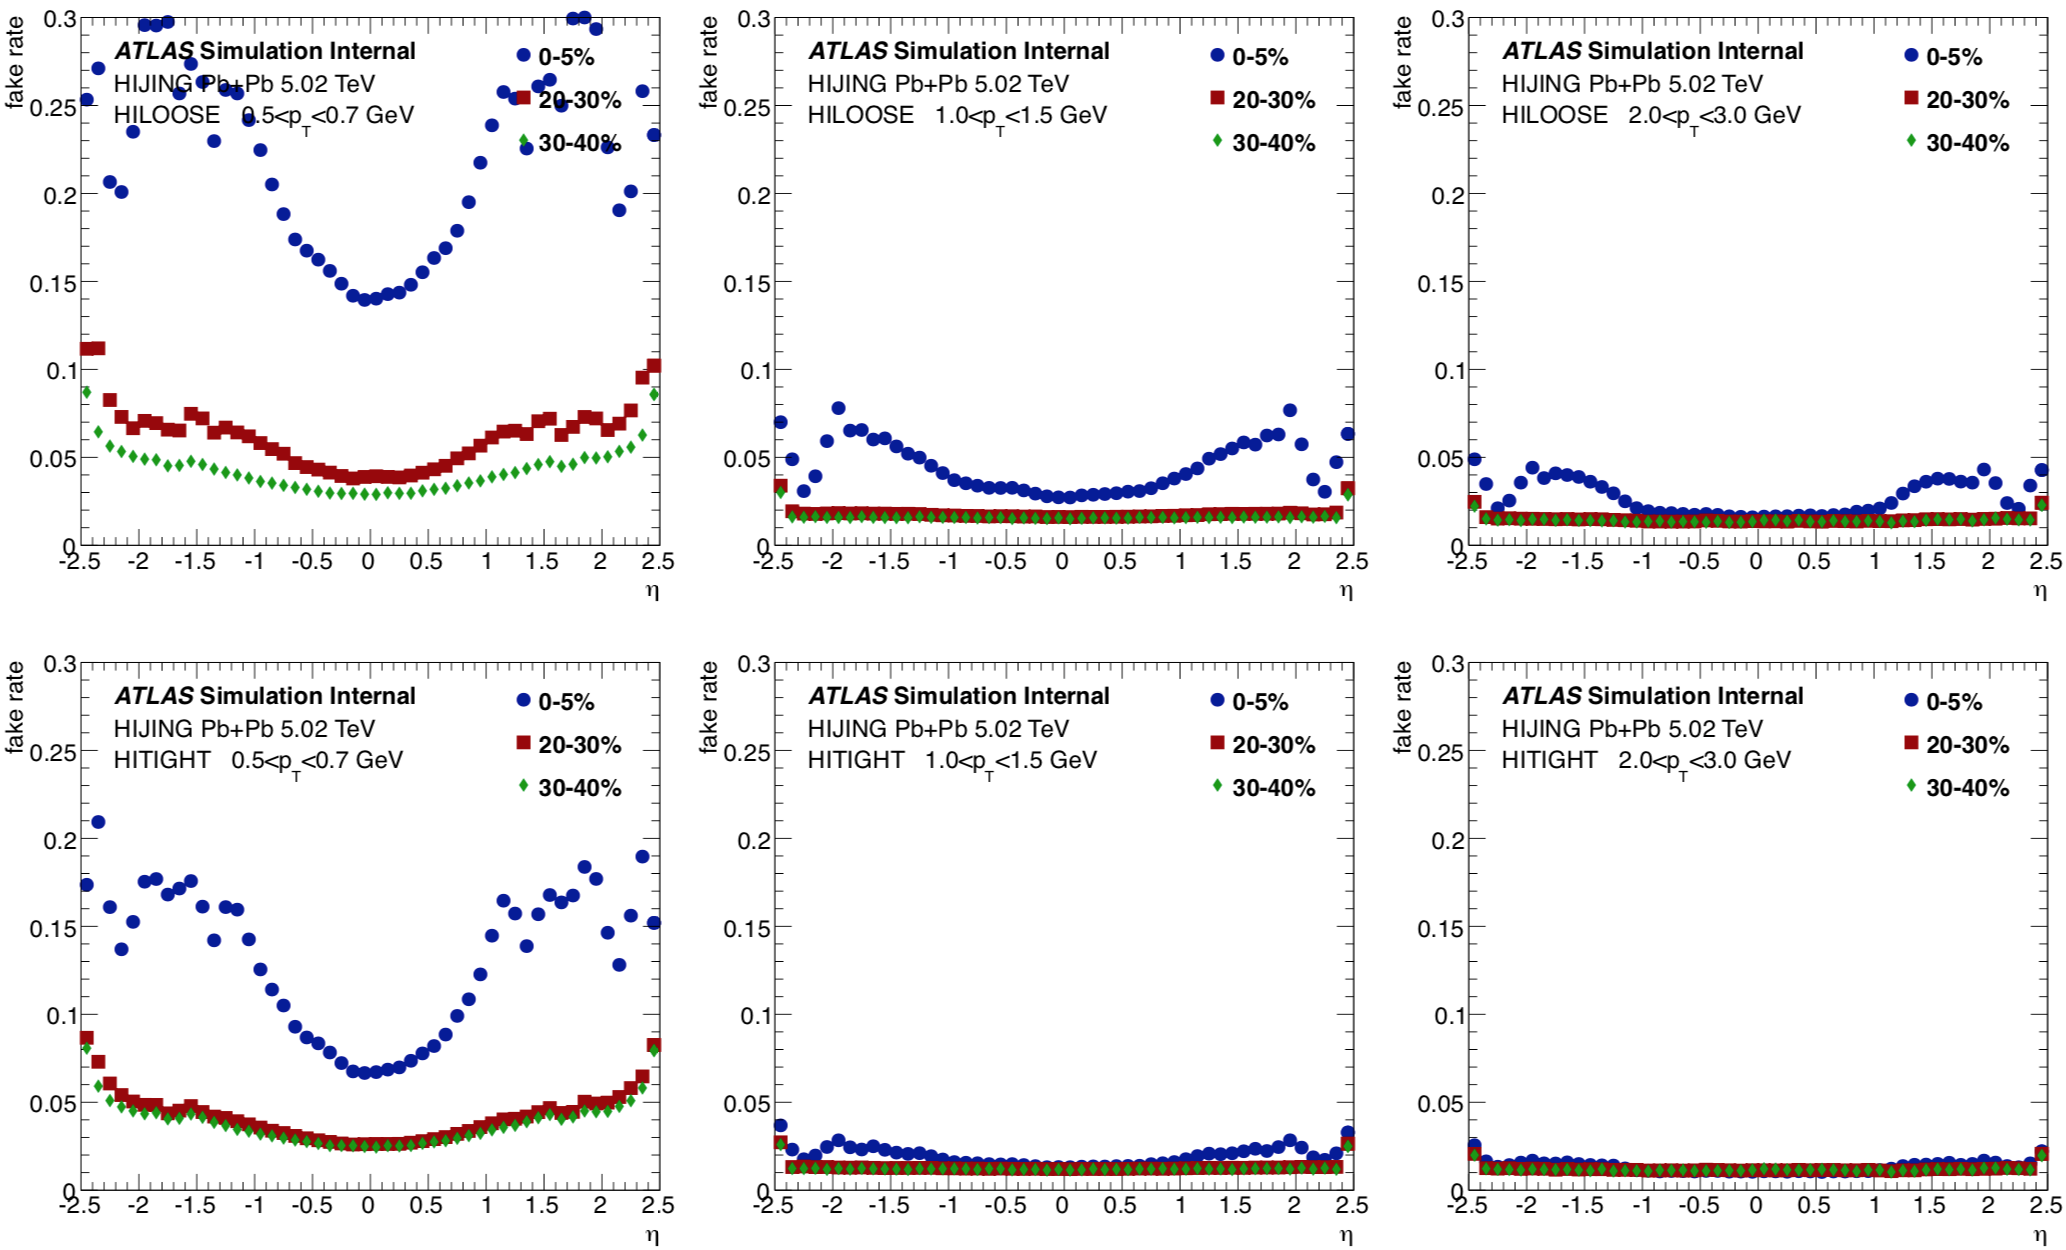
\includegraphics[width=.95\linewidth]{figs/chapter_detector/ATLAS_track_fake_PbPb502.png}
\caption{5.02 TeV Pb+Pb tracking fake rates $f(\eta)$, for different $\pT$ ranges and centralities. Top row is for HILoose and bottom row is for HITight.}
\label{fig:detector_ATLAS_track_fake_PbPb502}
\end{figure}

To compensate the contribution from fake tracks, the efficiency $\epsilon$ can be corrected by defining $\epsilon'$:
\begin{equation}
\epsilon'(\pT, \eta, \text{centrality}) \equiv \frac{N_\text{ch}^\text{primary} + N_\text{ch}^\text{fake}}{N_\text{ch}^\text{truth}} = \frac{\epsilon}{1+f}
\end{equation}
where an additional correction of fake rates $1-f$ is added to the tracking efficiency $\epsilon$. In the analysis, we varied the tracking efficiency within its uncertainties to test the stability of the measurements, and the results are shown in Section~\ref{sec:tracking_efficiency}.



\subsubsection{Xe+Xe at $\sqrt{s_\text{NN}}=5.44$ TeV}

The Xe+Xe analysis uses data from the 2017 LHC Xe+Xe run at $\sqrt{s_\text{NN}}=5.44$ TeV. The data were recorded during a single 8 hour fill in October 2017. The data were recorded into several streams. This analysis uses data from the MinBias stream only.



\paragraph{Trigger}

The MinBias events were recorded by the following two triggers:
\begin{itemize}
\item \verb|HLT_mb_sptrk_L1MBTS_1_VTE4|: At level-1, this trigger requires less than 4 GeV transverse energy in the calorimeter together with a signal in one of the MBTS detectors. At the high level trigger, this requires one reconstructed track. This trigger is meant to select peripheral events;
\item \verb|HLT_noalg_mb_L1TE4|: This trigger simply requires that the L1 transverse energy to be greater than 4 GeV;
\end{itemize}

During the data collection, none of the events passed \verb|L1VTE4| without prescale, and the prescale value varies between 3.3 and 8.0. On the other hand, all the events passed \verb|L1TE4| trigger without prescaling. To properly include the events that passed trigger \verb|L1VTE4|, an event weight $w_\text{trig}$ has been applied to the measured observable. As a summary, the FCal $\Et$ distributions with different trigger selections are shown in Figure~\ref{fig:detector_ATLAS_trigger_XeXe544}. Without $w_\text{trig}$ weight, the combined distribution shows a depletion for FCal $\Et<40$ GeV, which disappears after $w_\text{trig}$ is applied. Since the prescale for \verb|L1TE4| is one, with and without $w_\text{trig}$ weighting have no effects on the $\Et$ distribution.

\begin{figure}[H]
\centering
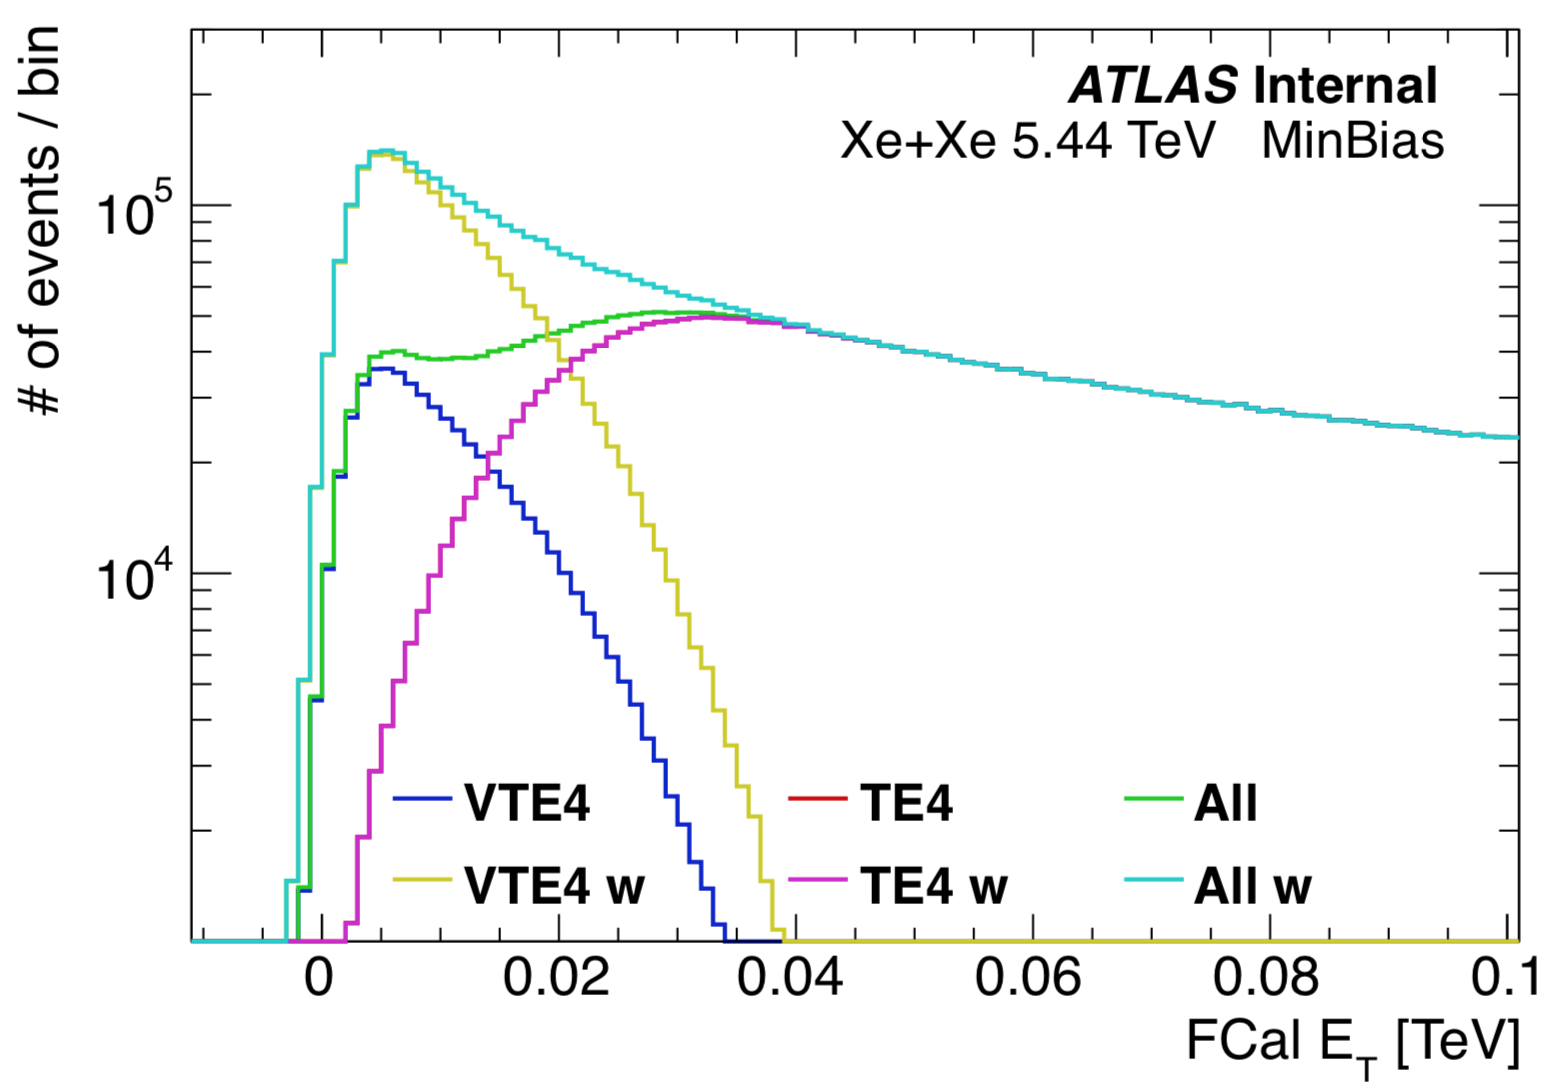
\includegraphics[width=.6\linewidth]{figs/chapter_detector/ATLAS_trigger_XeXe544.png}
\caption{FCal $\Et$ distributions with different trigger selections. ``All'' combines the events passing L1VTE4 and L1TE4. ``w'' meas the distributions are $w_\text{trig}$ weighted.}
\label{fig:detector_ATLAS_trigger_XeXe544}
\end{figure}



\paragraph{Event selection}

The basic event selection of Xe+Xe is exactly the same as Pb+Pb, as discussed in Section~\ref{sec:event_selection}.

During the Xe+Xe run the peak $\mu$ is about 0.00019 and the peak luminosity is 0.000211e30 $\text{cm}^{-2}\text{s}^{-1}$, thus the expected fraction of pileup events is not high. In this analysis pileup rejection is done utilizing the tight correlation between the FCal $\Et$ and the number of reconstructed tracks associated with the primary vertex, as shown in Figure~\ref{fig:detector_ATLAS_FCal_Nch_XeXe544}. The tightly correlated band seen along the diagonal is the correlation from events with a single vertex. Pileup events typically have a much larger FCal $\Et$ at the same value of $\Nchrec$, since $\Nchrec$ denotes the number of tracks associated with the primary vertex and is not affected by pileup. While the FCal $\Et$ is larger due to the additional tracks from the pileup vertex. The pileup events can be rejected by removing events with large FCal $\Et$, at a given $\Nchrec$ such that the event lies outside the tight correlation band between the $\Nchrec$ and the FCal $\Et$. This is shown in Figure~\ref{fig:detector_ATLAS_FCal_Nch_XeXe544} by the red lines. The fraction of events rejected by this cut is approximately $0.1\%$. This cut does not reject pileup events where the FCal $\Et$ is only modified slightly such that they fall within the diagonal band. However, including such events does not affect the analysis, as they only have slightly wrong values of FCal $\Et$ assigned to them, and therefore have only a small error in the assigned centrality.

\begin{figure}[H]
\centering
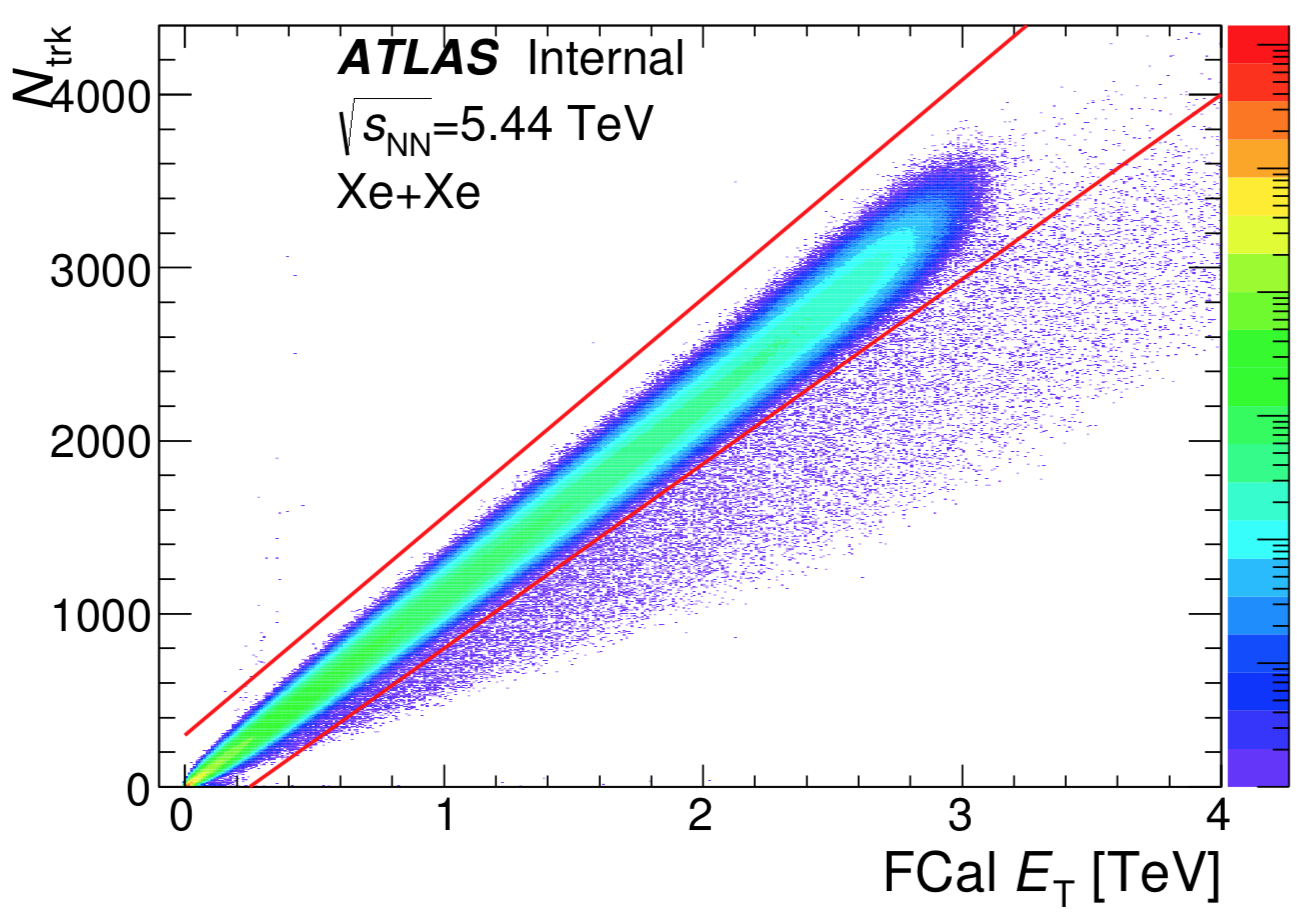
\includegraphics[width=.6\linewidth]{figs/chapter_detector/ATLAS_FCal_Nch_XeXe544.png}
\caption{The correlation between FCal $\Et$ and the number of reconstructed tracks (without any restriction on $\pT$ or quality). The red lines show fiducial cuts to reject pileup and other bad events.}
\label{fig:detector_ATLAS_FCal_Nch_XeXe544}
\end{figure}



\paragraph{Centrality determination}

The MinBias events are binned into centrality percentiles based on the FCal $\Et$. The left panel of Figure~\ref{fig:detector_ATLAS_centrality_XeXe544} shows the FCal $\Et$ distribution for the events used in this analysis, together with the defined centrality classes. The right panel shows the centrality distributions for the MinBias events.

\begin{figure}[H]
\centering
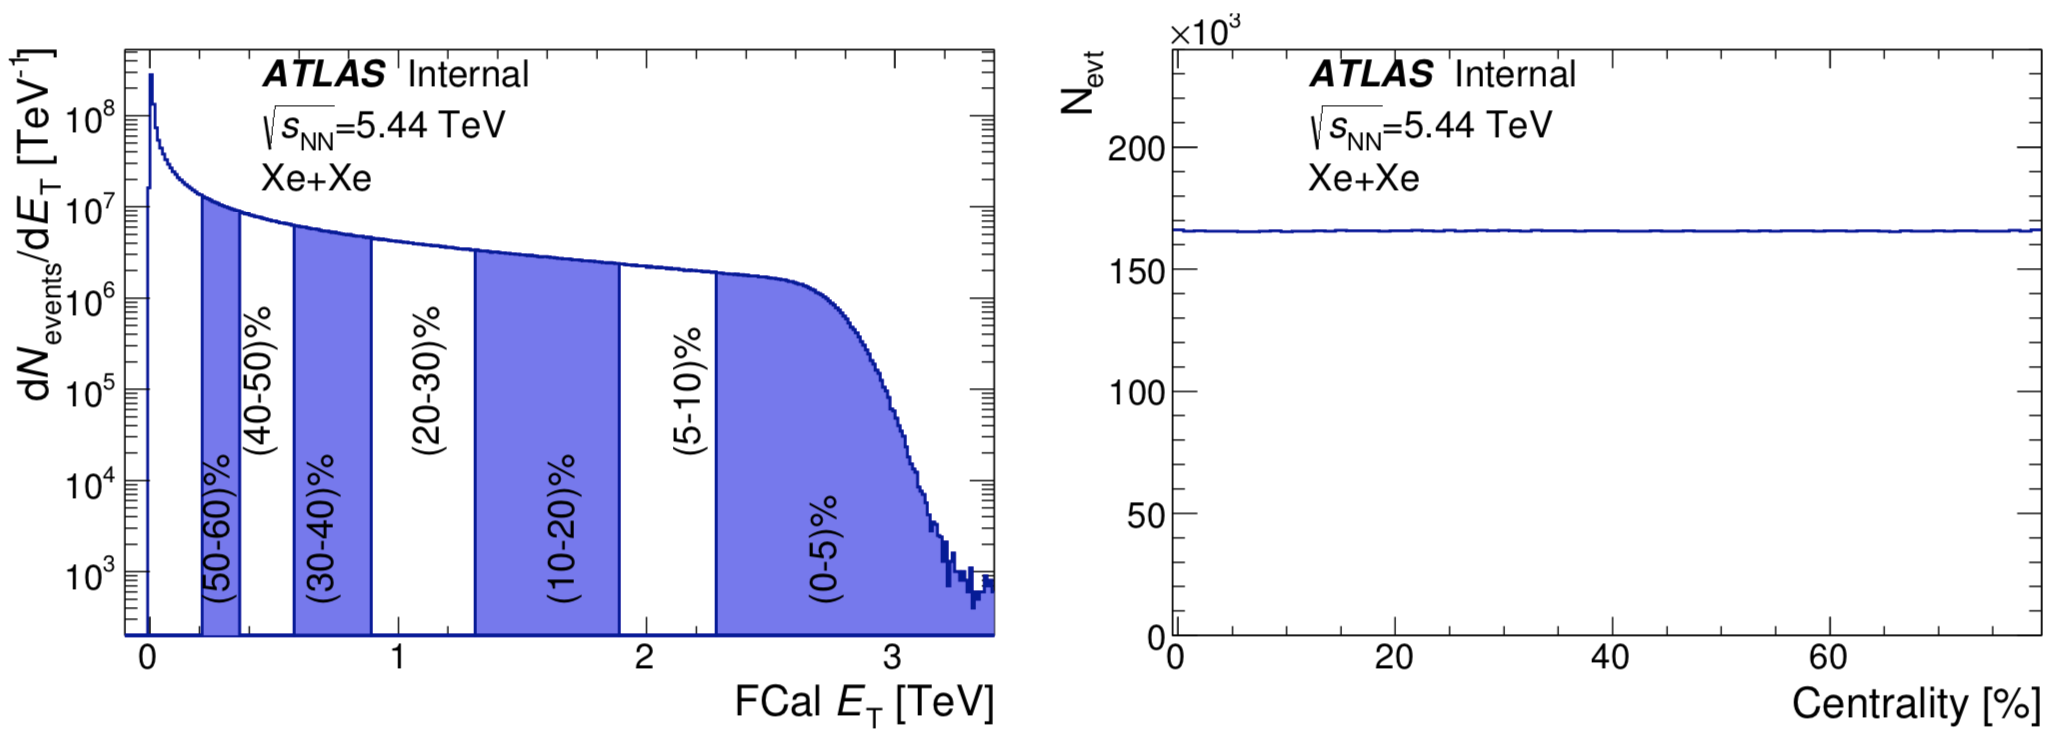
\includegraphics[width=.95\linewidth]{figs/chapter_detector/ATLAS_centrality_XeXe544.png}
\caption{Left: The FCal $\Et$ distribution in MinBias events together with the binning used to define some of the centrality classes. Right: The centrality distribution for MinBias events over the $0-80\%$ centrality interval.}
\label{fig:detector_ATLAS_centrality_XeXe544}
\end{figure}

It is interesting to note that the FCal $\Et$ distribution for the Xe+Xe events has a very similar shape to that seen in previously shown Pb+Pb events. This is shown in Figure~\ref{fig:detector_ATLAS_centrality_XePb}, where after scaling the Pb+Pb FCal $\Et$ distribution by an empirical factor of 0.65, it nearly coincides with the Xe+Xe distribution. It is also interesting to note that the number of nucleons in Xe+Xe is approximated 0.62 (129/208) of the number of nucleons in Pb. Nonetheless, an independent centrality cuts were established for Xe+Xe.

\begin{figure}[H]
\centering
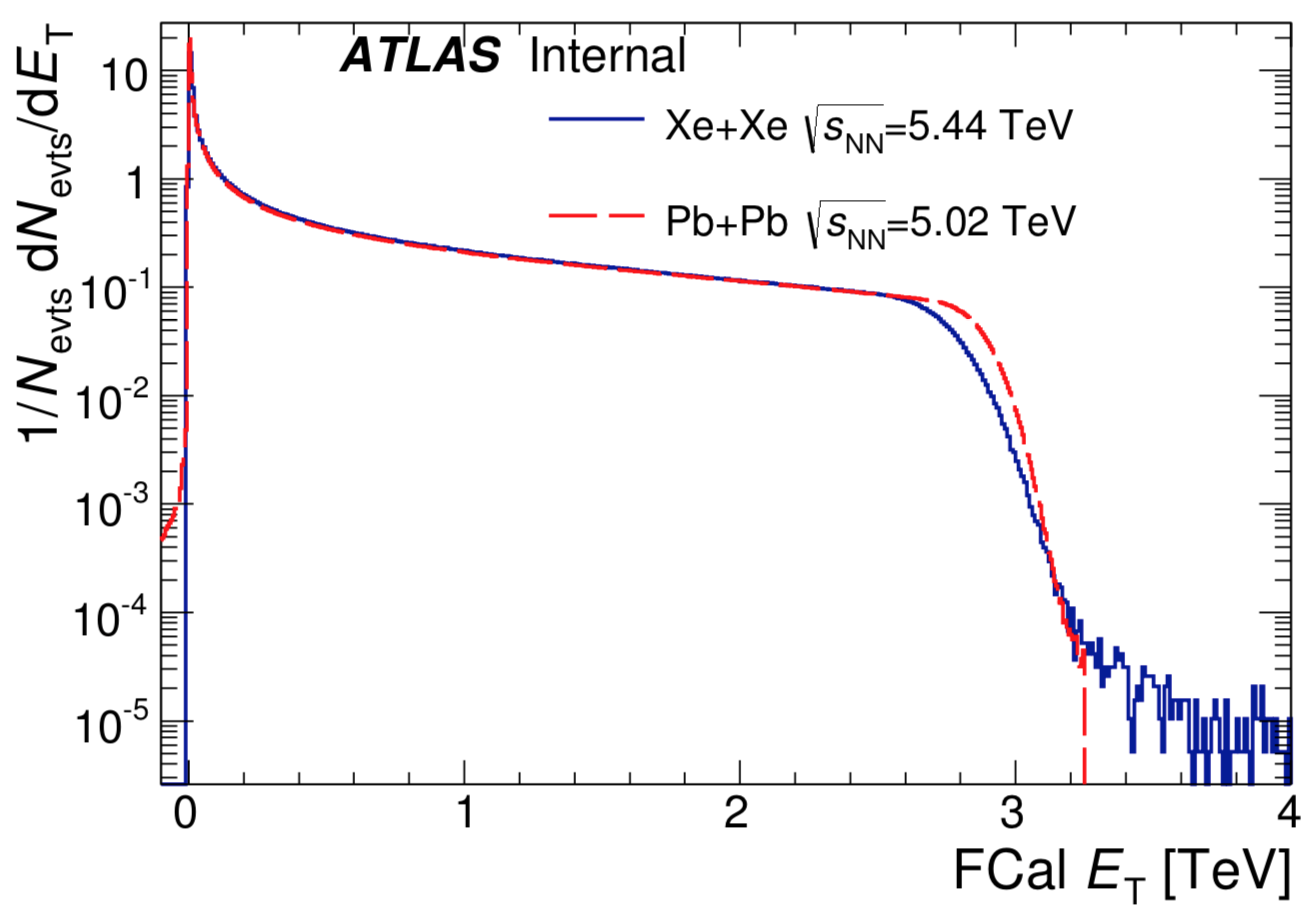
\includegraphics[width=.6\linewidth]{figs/chapter_detector/ATLAS_centrality_XePb.png}
\caption{Comparison between the FCal $\Et$ distribution in Pb+Pb events at $\sqrt{s_\text{NN}}=5.02$ TeV, and the Xe+Xe events at $\sqrt{s_\text{NN}}=5.44$ TeV. The $\Et$ distribution for Pb+Pb events is scaled by an empirical factor of 0.65.}
\label{fig:detector_ATLAS_centrality_XePb}
\end{figure}



\paragraph{Track selection, efficiency and fake rate}

The track selection for Xe+Xe is exactly same as Pb+Pb discussed in previous section. Performance of tracking cuts was established in the MC sample of simulated one million HIJING events. The tracking performance depends on the overall event activity (especially the fake rate) therefore it is obtained from the MC events of similar multiplicities to data. For that, for each centrality bin in data the track multiplicity was obtained. Then efficiency and fake rates were obtained from MC for matching multiplicities. The procedure is identical to the one used for Pb+Pb data described in previous section. Figure~\ref{fig:detector_ATLAS_track_eff_XeXe544} and Figure~\ref{fig:detector_ATLAS_track_fake_XeXe544} show efficiency and fake rates, for different $\pT$, $\eta$ and centrality ranges.

\begin{figure}[H]
\centering
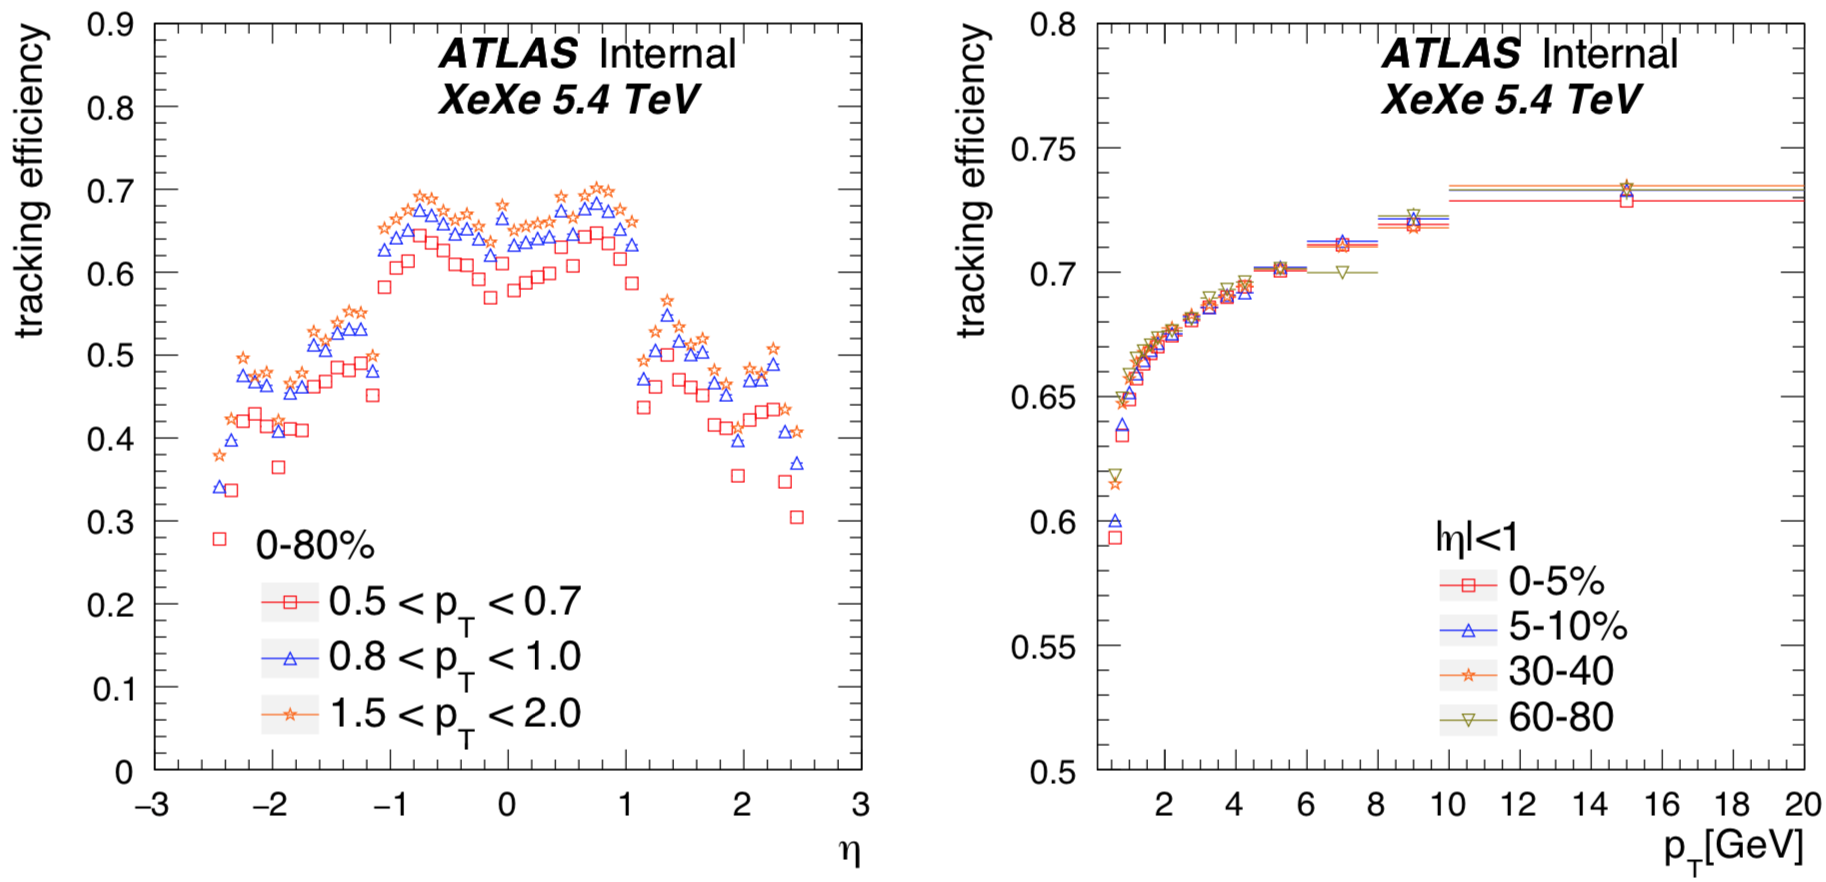
\includegraphics[width=.95\linewidth]{figs/chapter_detector/ATLAS_track_eff_XeXe544.png}
\caption{Tracking efficiency as a function of $\eta$ (left) and $\pT$ (right) for selected centrality and $\pT$ ranges.}
\label{fig:detector_ATLAS_track_eff_XeXe544}
\end{figure}

\begin{figure}[H]
\centering
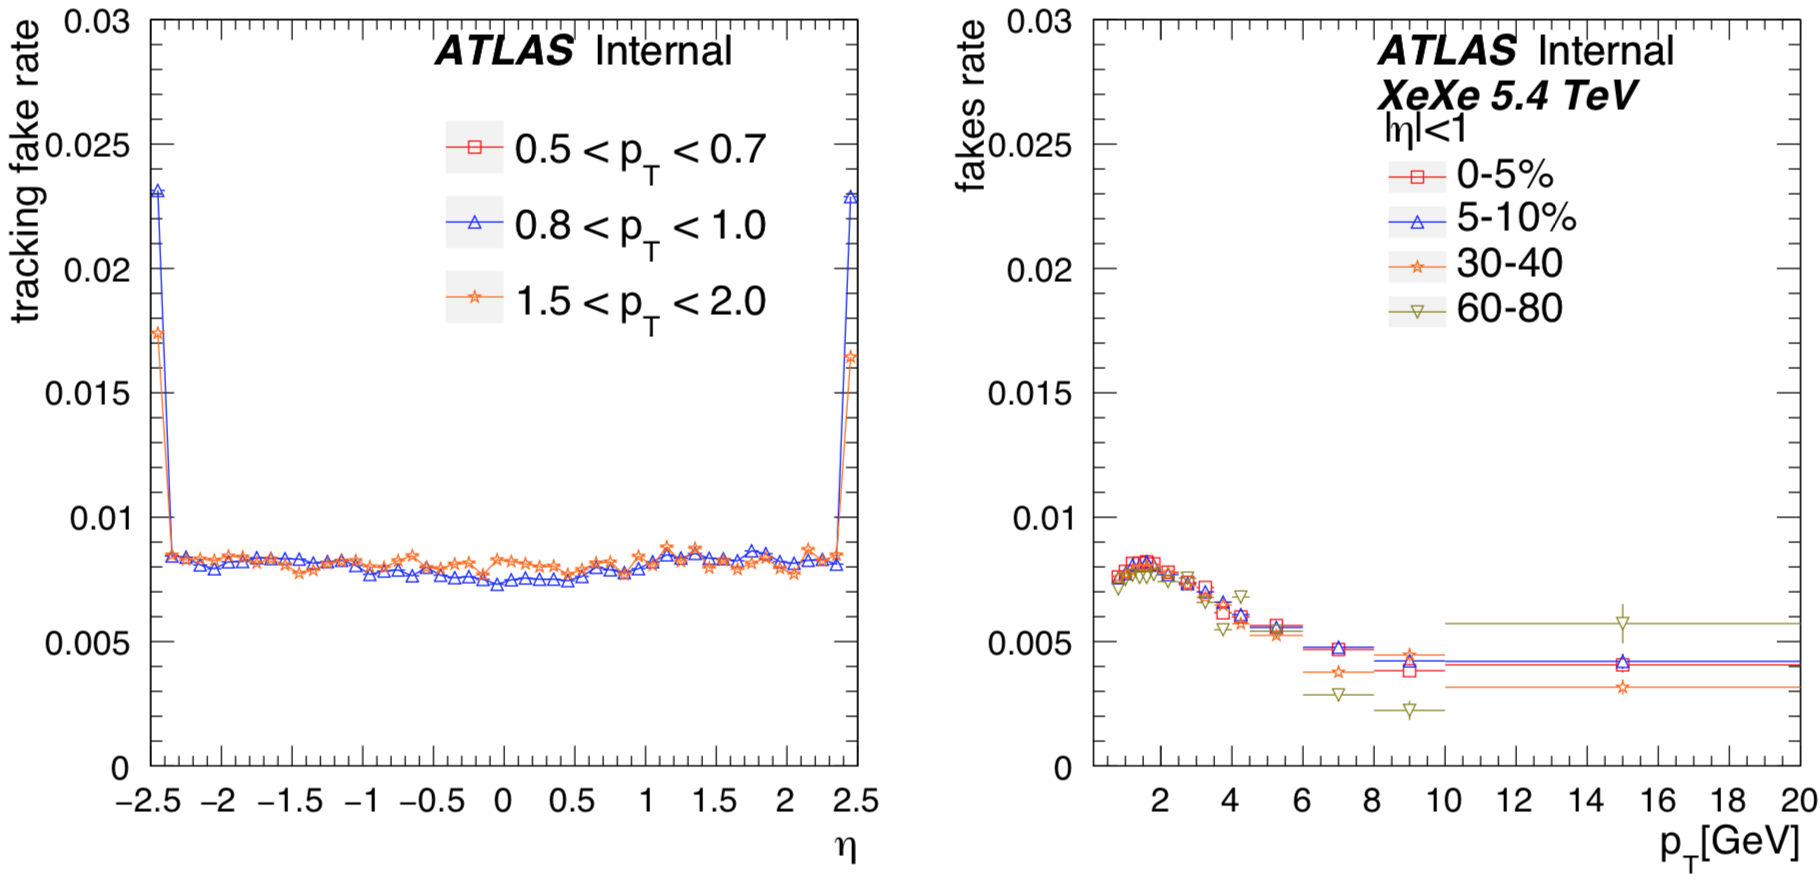
\includegraphics[width=.95\linewidth]{figs/chapter_detector/ATLAS_track_fake_XeXe544.png}
\caption{Fake rates as a function of $\eta$ (left) and $\pT$ (right) for selected centrality and $\pT$ ranges. The $\eta$ dependence is shown for $10\%$ most central events, where fake rate is highest.}
\label{fig:detector_ATLAS_track_fake_XeXe544}
\end{figure}



\subsubsection{$p$+Pb at $\sqrt{s}=5.02$ TeV}

$p$+Pb data at $\sqrt{s}=5.02$ TeV data have been collected in 2013 (Run 1) and 2016 (Run 2). Since the event and tracking selections are quite different between Run 1 and Run 2, they will be discussed separately in the following sections.



\paragraph{Trigger}

The triggers applied in 5.02 TeV $p$+Pb have two parts: MinBias and High Multiplicity Track (HMT). A list of all the major MinBias and HMT triggers used in 2013 is summarized as follows:
\begin{itemize}
\item \verb|EF_mbMbts_1_1_counter|
\item \verb|EF_hip_trkX_TEY_counter|
\end{itemize}
where two new algorithms are used:
\begin{itemize}
\item \verb|mbMbts_1_1|: HLT trigger requires at least 1 hit on both sides of MBTS;
\item \verb|trkX|: HLT trigger requires at least X online reconstructed tracks;
\end{itemize}
The threshold combinations $(X, Y)$ for number of tracks (\verb|trk|) and total energy (\verb|TE|) are (100, 10), (130, 10), (150, 50), (185, 50), (200, 65) and (225, 65).

A summary of statistics with all the major triggers used in this thesis are shown in Figure~\ref{fig:detector_ATLAS_trigger_pPb2013}.
\begin{figure}[H]
\centering
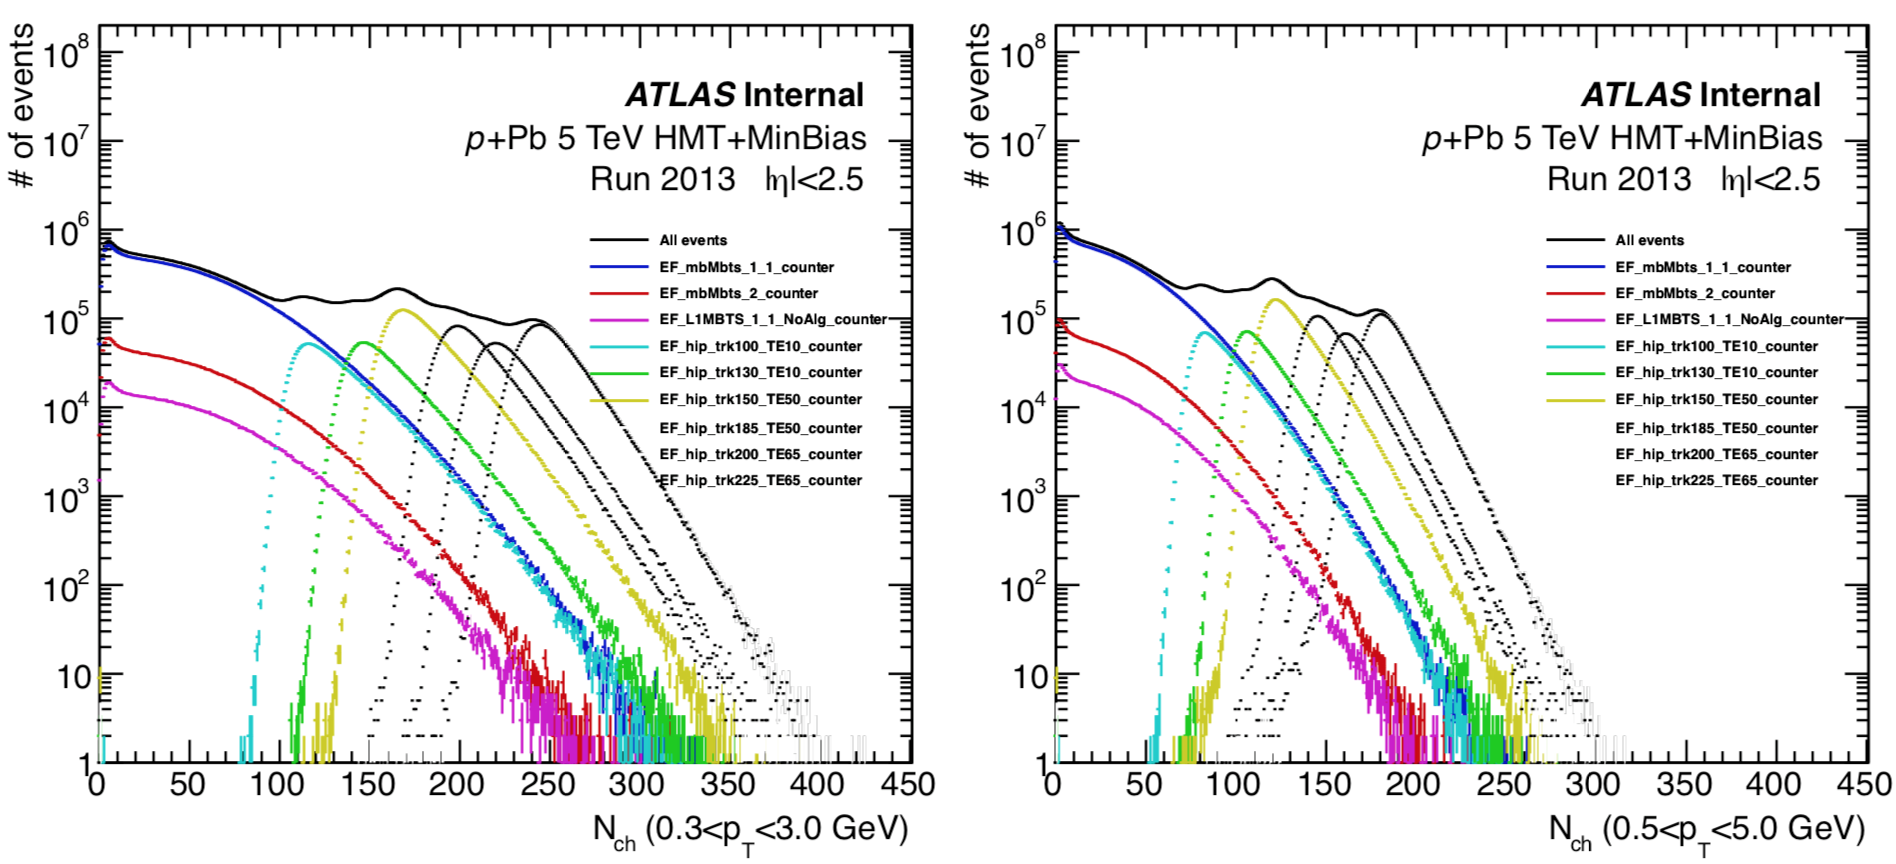
\includegraphics[width=.95\linewidth]{figs/chapter_detector/ATLAS_trigger_pPb2013.png}
\caption{Distributions of number of tracks with two $\pT$ thresholds, for 5.02 TeV $p$+Pb run in 2013. The major MinBias and HMT triggers are plotted separately.}
\label{fig:detector_ATLAS_trigger_pPb2013}
\end{figure}

Due to the reason that the intermediate $\Nchrec$ region is not covered by the 2013 HMT triggers, several new HMT triggers with intermediate $\Nchrec$ thresholds are specially designed for the 2016 data taking. Together with MinBias triggers, all the major triggers used in this thesis are summarized as follows:
\begin{itemize}
\item \verb|HLT_noalg_mb_L1MBST_1|
\item \verb|HLT_noalg_mb_L1MBST_1_1|
\item \verb|HLT_mb_sp100_trkX_hmt_L1MBST_1_1|
\end{itemize}
where all the HMT triggers are seeded on \verb|L1MBTS_1_1|, which is different from 2013 since the luminosity is much lower. The new algorithms are:
\begin{itemize}
\item \verb|L1MBST_1| requires at least one hit in one of the MBST detectors;
\item \verb|L1MBST_1_1| requires at least one hit in both of the MBST detectors;
\item \verb|sp100| requires at least 100 space points in for the HLT track reconstruction.
\end{itemize}
The thresholds $X$ for number of tracks (\verb|trk|) are 10, 20, 30, 60, 80, 100 and 110.

The summary of statistics with all the major triggers used in this thesis are shown in Figure~\ref{fig:detector_ATLAS_trigger_pPb2016}.
\begin{figure}[H]
\centering
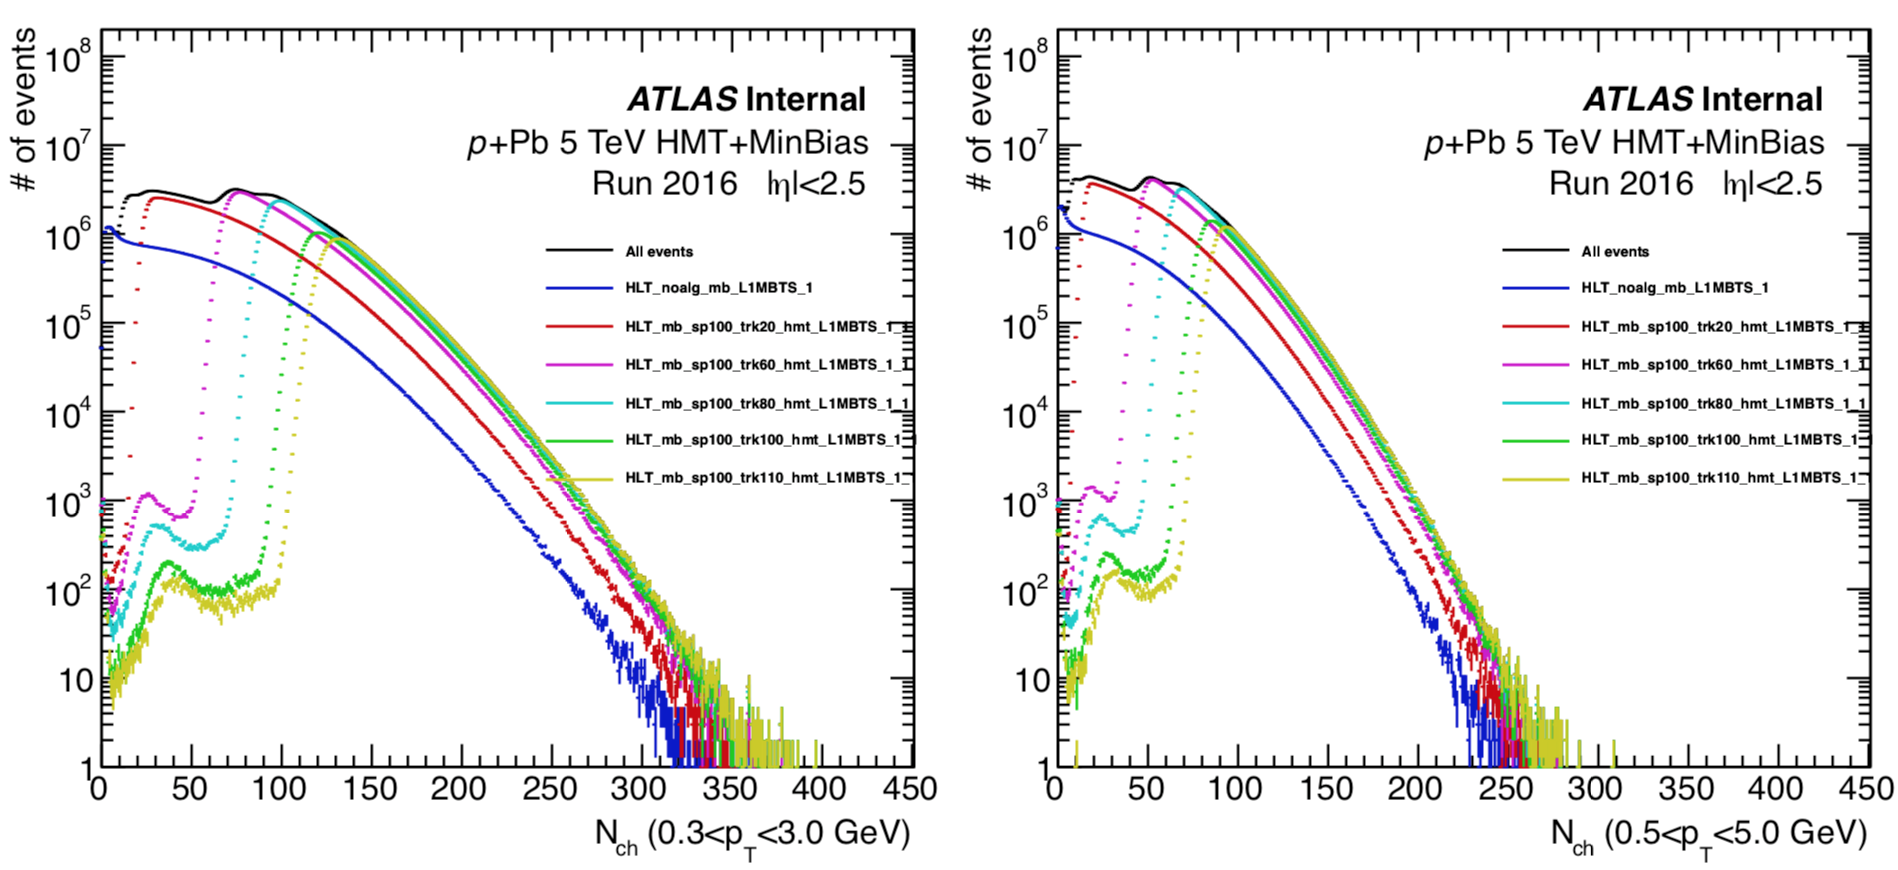
\includegraphics[width=.95\linewidth]{figs/chapter_detector/ATLAS_trigger_pPb2016.png}
\caption{Distributions of number of tracks with two $\pT$ thresholds, for 5.02 TeV $p$+Pb run in 2016. The major MinBias and HMT triggers are plotted separately.}
\label{fig:detector_ATLAS_trigger_pPb2016}
\end{figure}



\paragraph{Event selection}

In 2013, low-$\mu$ 5.02 TeV $p$+Pb data were collected with the ATLAS detectors. Each event is required to pass the following cuts:
\begin{itemize}
\item Good run list;
\item A primary reconstructed vertex with $z_\text{vtx}<100$ mm;
\item MBTS timing cuts
\begin{itemize}
\item $|\text{time}_\text{A}|$ or $|\text{time}_\text{C}|$ must not be equal to 75 or 0 ns;
\item $|\text{time}_\text{A} - \text{time}_\text{C}|<10$ ns;
\end{itemize}
\end{itemize}
and the pileup events are suppressed by rejecting events containing more than one good reconstructed vertex. The remaining pileup events are further suppressed based on the signal in the ZDC on the Pb-fragmentation side. This signal is calibrated to the number of detected neutrons $N_\text{n}$ based on the location of the peak corresponding to a single neutron. The distribution of $N_\text{n}$ in events with pileup is broader than that for events without pileup. Hence, a simple cut on the high tail end of the ZDC signal distribution further suppresses the pileup, which retaining more than $98\%$ of the events without pileup. After this pileup rejection procedure, the residual fraction is estimated to be $1\%$ in the event class with the highest track multiplicity studied in this analysis.

In 2016, 5.02 TeV $p$+Pb data was collected with lower $\mu$ value than 2013. In addition to the event selections in 2013 (without MBTS timing cuts), events with problematic detectors are also removed. Since $\mu$ value of 2016's run is much lower than 2013's, cleaning pileup events is not crucial.



\paragraph{Track selection, efficiency and fake rate}

The track selection criteria for 2016 $p$+Pb is quite different from Pb+Pb. The analysis uses the $p$+Pb data reprocessed with the tracking extended down to 0.1 GeV:
\begin{itemize}
\item Present hit in B-Layer if expected
\item Number of Pixel hits $\geq 1$
\item SCT hits:
\begin{itemize}
\item SCT hits $\geq$ 2 for $0.1 < \pT < 0.2$ GeV
\item SCT hits $\geq$ 4 for $0.2 < \pT < 0.3$ GeV
\item SCT hits $\geq$ 6 for $\pT > 0.3$ GeV
\end{itemize}
\item significance cuts:
\begin{itemize}
\item $|\frac{d_0}{err_{d_0}}|<3$
\item $|\frac{z_0\sin\theta}{err_{z_0\sin\theta}}|<3$
\end{itemize}
\end{itemize}

Tracking efficiency is estimated in a similar way as Pb+Pb. The tracking efficiency evaluated as a function of $\eta$ for different $\pT$ ranges compared between different multiplicity ranges are shown in Figure~\ref{fig:detector_ATLAS_track_eff_pPb}. The efficiency is lower in the lowest $\pT$ range ($0.1<\pT<0.2$ GeV), but changes weakly with increase in the $\pT$ above that. The $\eta$ dependence of the efficiency is also different the lowest $\pT$ range, but remains nearly consistent in the highest $\pT$ ranges. The $\eta$ dependence of the efficiency is also much weaker than that seen in central Pb+Pb collisions. Efficiency shows very weak dependence with multiplicity although the lowest multiplicity ranges shows a lightly lower efficiency than the rest of the multiplicity ranges.

\begin{figure}[H]
\centering
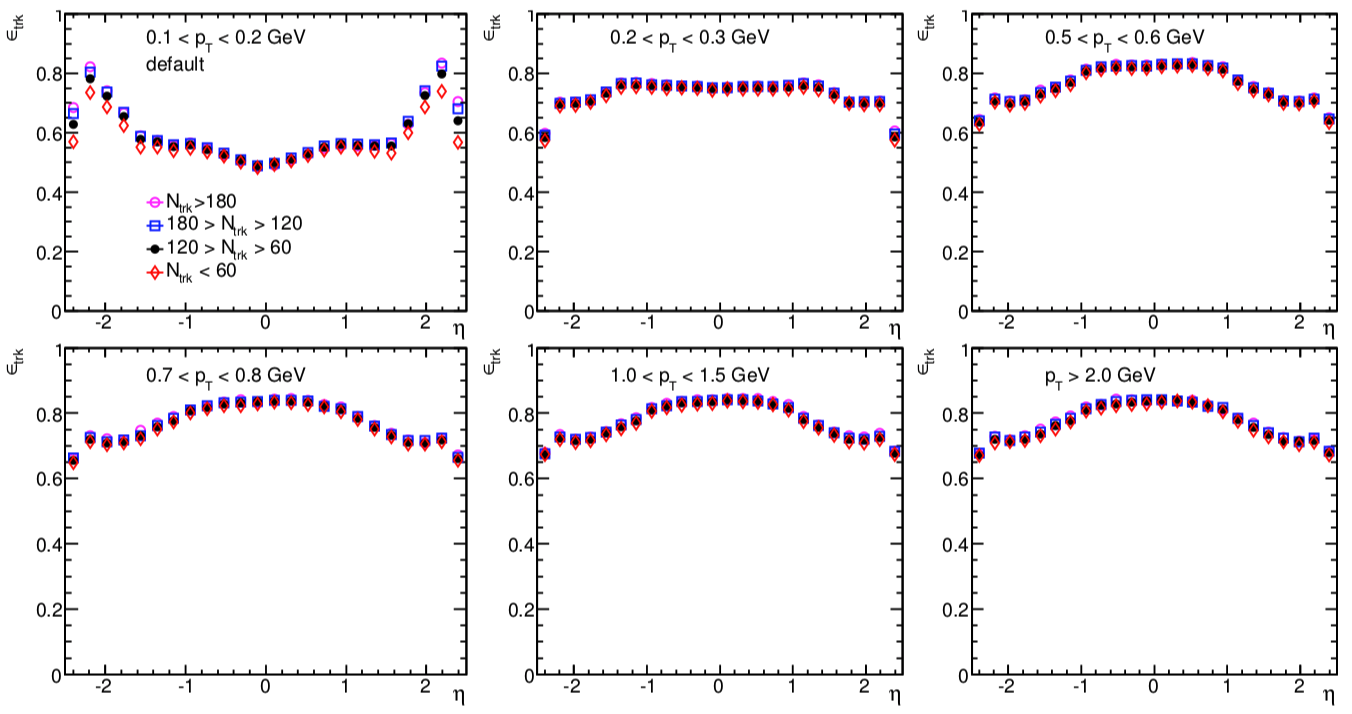
\includegraphics[width=.95\linewidth]{figs/chapter_detector/ATLAS_track_eff_pPb.png}
\caption{Tracking efficiency $\epsilon$ as a function of $\eta$ for default selection requirements for different transverse momentum $\pT$ ranges compared between different multiplicity bins, for $p$+Pb.}
\label{fig:detector_ATLAS_track_eff_pPb}
\end{figure}



\subsubsection{$pp$ at $\sqrt{s}=13$ TeV}

In 2015 and 2016, low-$\mu$ and intermediate-$\mu$ $pp$ data was collected by ATLAS detectors. An additional pixel layer, the ``Insertable B Layer'' (IBL) installed between Run 1 and Run 2, is used in the $pp$ measurement. There are four run periods depending on the triggers and will be discussed below.



\paragraph{Trigger}

The triggers that have been used in this analysis have both MinBias and HMT triggers. The HMT triggers are developed to enhance event statistics in high multiplicity region. Since the main uncertainty in many measurements, like cumulants, are from statistical errors, HMT triggers are crucial in order to extend the measurement to higher multiplicity region. The list of all major triggers used are listed as follows:
\begin{itemize}
\item \verb|HLT_mb_sptrk|
\item \verb|HLT_noalg_mb_MBTS_1|
\item \verb|HLT_noalg_mb_MBTS_1_1|
\item \verb|HLT_mb_mbts_L1MBTS_1_1|
\item \verb|HLT_mb_sp400_trk40_hmt_L1MBTS_1_1|
\item \verb|HLT_mb_sp900_trk50_hmt_L1TE5|
\item \verb|HLT_mb_sp900_trk60_hmt_L1MBTS_1_1|
\item \verb|HLT_mb_sp1000_trk70_hmt_L1TE5|
\item \verb|HLT_mb_sp1400_trk90_hmt_L1TE10|
\end{itemize}

Figure~\ref{fig:detector_ATLAS_trigger_pp13} shows the distributions of number of tracks from two $\pT$ thresholds: $0.3<\pT<3.0$ GeV (left panel) and $0.5<\pT<5.0$ GeV (right panel). Due to a large number of HMT triggers, only selected triggers are shown.

\begin{figure}[H]
\centering
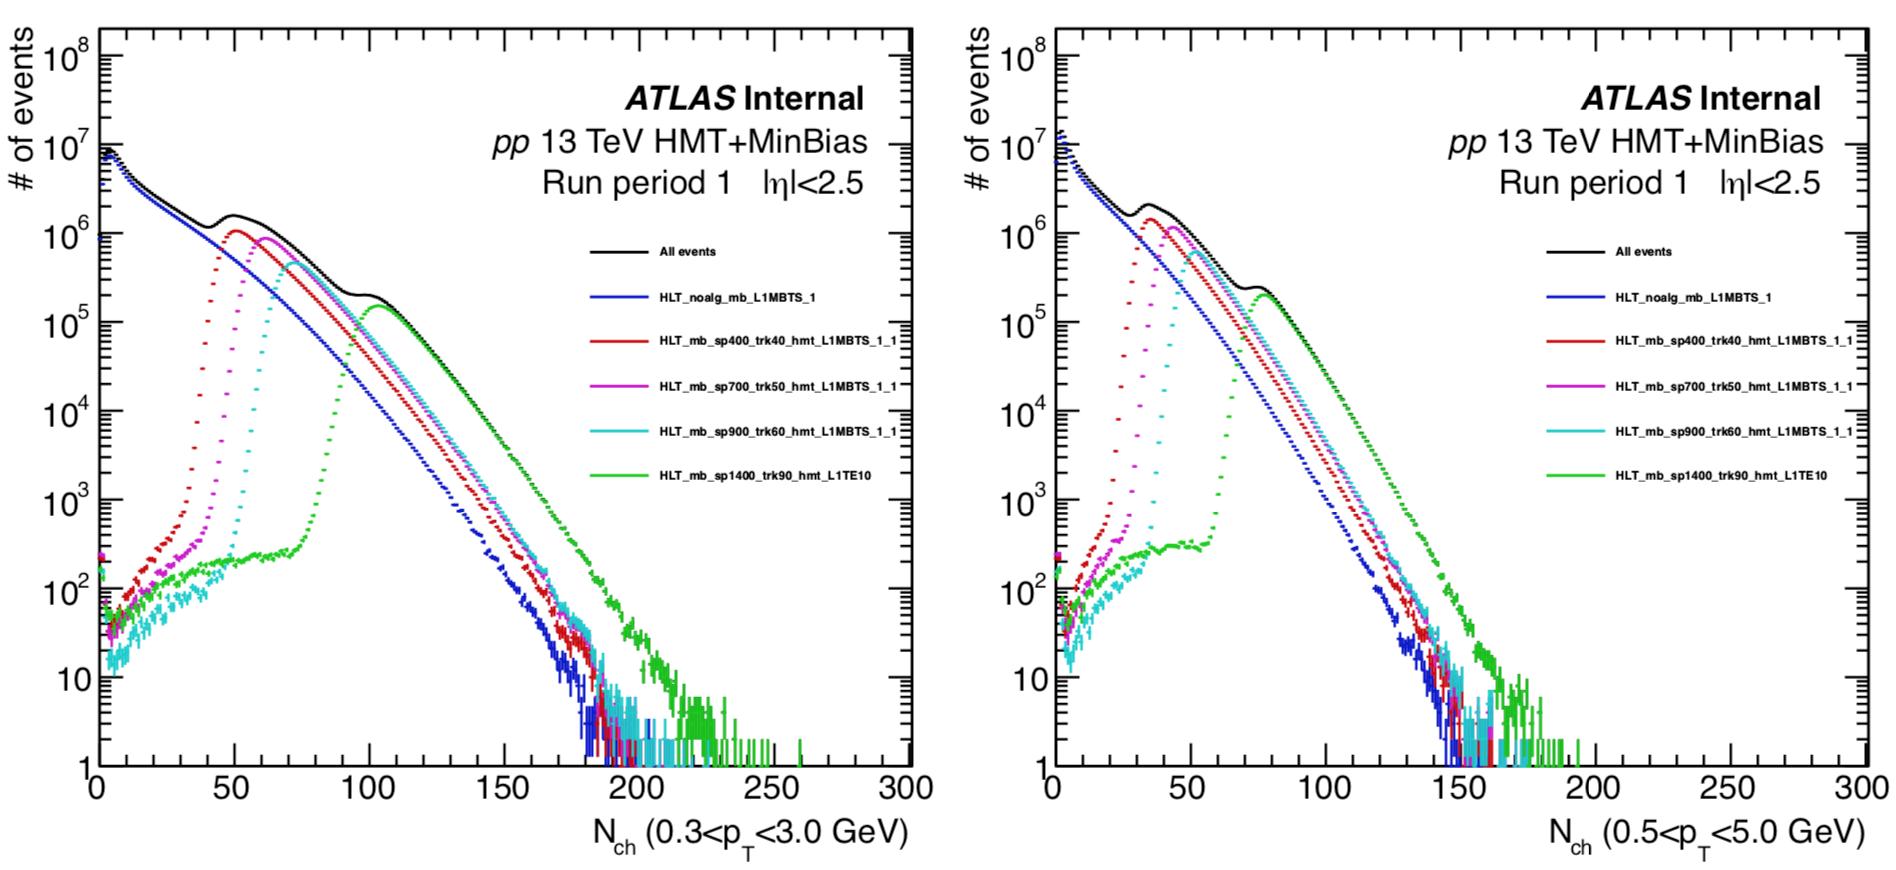
\includegraphics[width=.95\linewidth]{figs/chapter_detector/ATLAS_trigger_pp13.png}
\caption{Distributions of number of tracks with two $\pT$ thresholds, in 13 TeV $pp$, with selected MinBias and HMT triggers. "All events" means all the MinBias and HMT triggers combined.}
\label{fig:detector_ATLAS_trigger_pp13}
\end{figure}



\paragraph{Event selection}

The event selection criteria for $pp$ are exactly the same as Pb+Pb at $\sqrt{s_\text{NN}}=5.02$ TeV, see Section~\ref{sec:event_selection} for details.



\paragraph{Track selection, efficiency and fake rate}

The track selection for $pp$ is slightly different from $p$+Pb:
\begin{itemize}
\item If IBL hit is expected: at least 1 IBL hit;
\item If no IBL hit is expected: a Layer-0 hit if expected;
\item At least 1 pixel hit + dead sensors;
\item SCT hits:
\begin{itemize}
\item $\pT<0.3$ GeV: at least 2 SCT hits + dead sensors;
\item $\pT<0.4$ GeV: at least 4 SCT hits + dead sensors;
\item $\pT>0.4$ GeV: at least 6 SCT hits + dead sensors;
\end{itemize}
\item If $\pT>10$ GeV: $\chi^2$ probability < 0.01;
\item $|d_0|<1.5$;
\item $|z_0-z_\text{vtx}|\sin\theta<1.5$;
\end{itemize}

The PYTHIA A2 tune was used to produce $pp$ collisions with the same energy as in the data. The detector response is simulated with GEANT 4 with conditions matching those present during the data-taking. The simulated events are reconstructed with the same algorithms as data, in particular using the same track reconstruction as for the data.

The definitions of tracking efficiency and fake rates are identical to the Pb+Pb collision system (Section~\ref{sec:track_selection_efficiency_and_fake_rate}). The tracking efficiency is shown in Figure~\ref{fig:detector_ATLAS_track_eff_pp13}. The boundaries of $\Nchrec$ are chosen to make each $\Nchrec$ range contain enough statistics for the efficiency measurement. The efficiency is higher in high multiplicity. Linear interpolation is applied in data analysis to obtain more precise efficiency in cases when $\pT$ or $\eta$ are not in the bin center.
\begin{figure}[H]
\centering
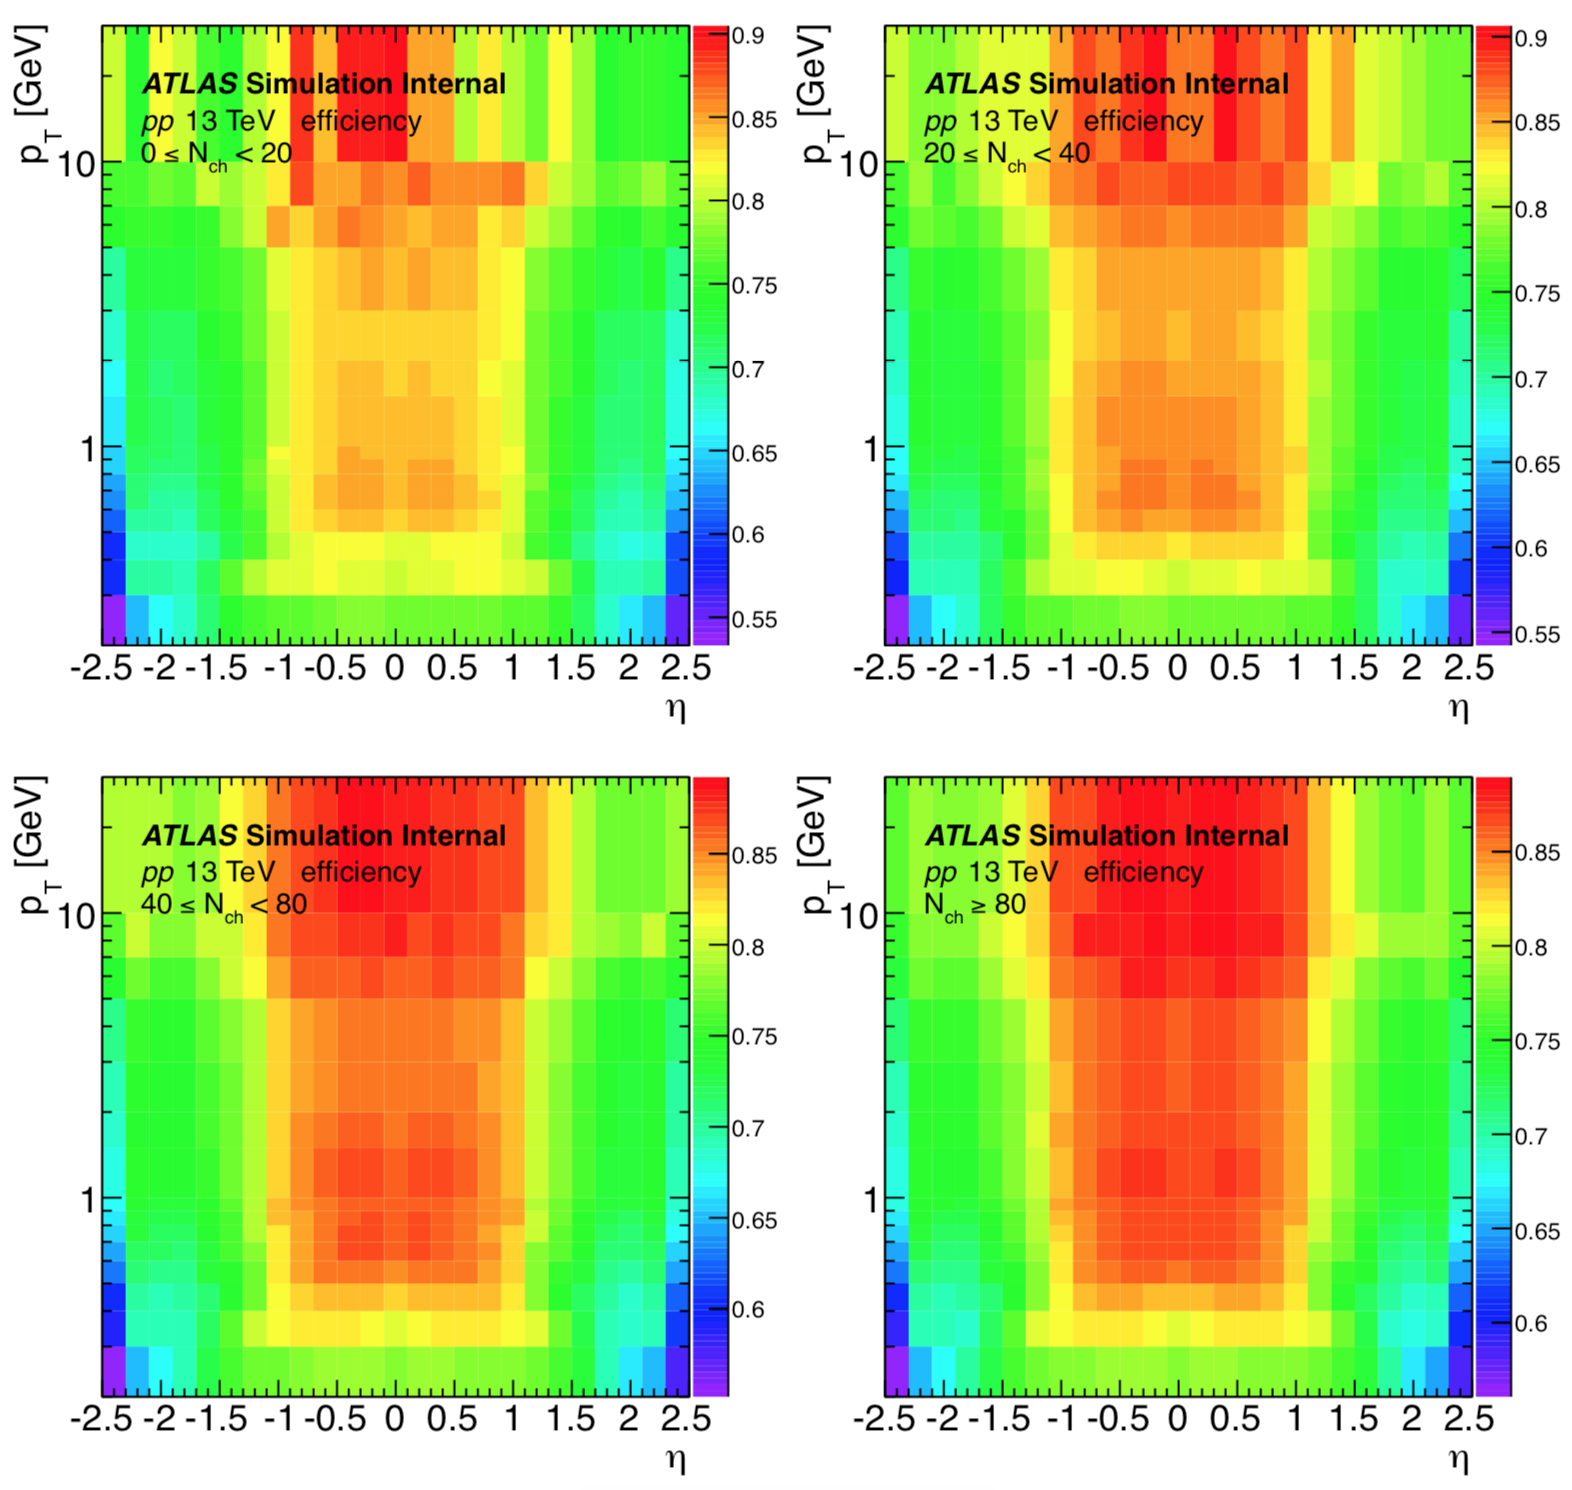
\includegraphics[width=.95\linewidth]{figs/chapter_detector/ATLAS_track_eff_pp13.png}
\caption{Tracking efficiency $\epsilon(\eta, \pT)$. Different panels are for different $\Nchrec$ ranges.}
\label{fig:detector_ATLAS_track_eff_pp13}
\end{figure}

The fake rates are shown in Figure~\ref{fig:detector_ATLAS_track_fake_pp13}, where four panels are for four different $\Nchrec$ ranges, respectively. Since the maximum fake rate is smaller than the level of $0.1\%$, even for the lowest $\pT$, unlike central Pb+Pb, fake rates have no impact on the $pp$ data analysis.
\begin{figure}[H]
\centering
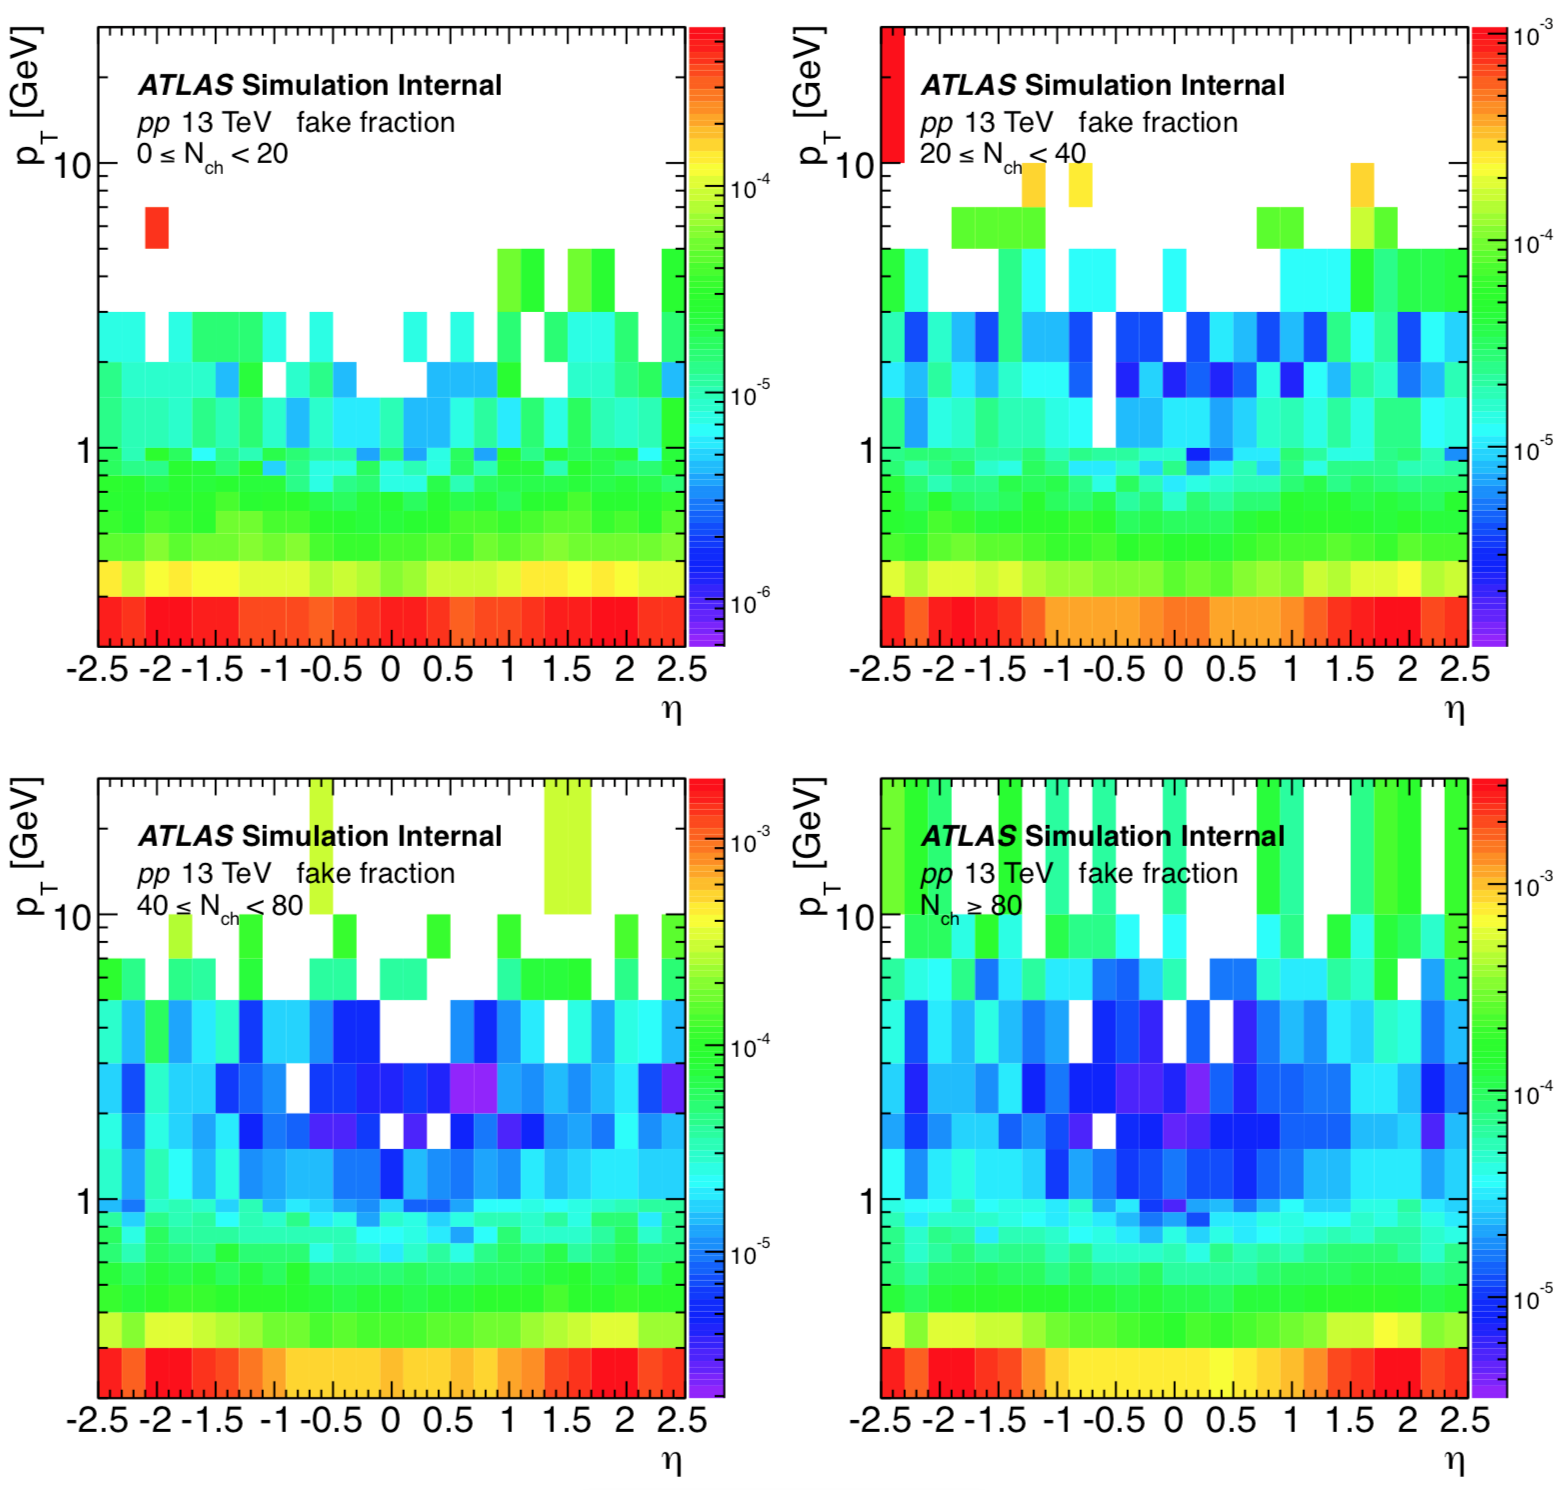
\includegraphics[width=.95\linewidth]{figs/chapter_detector/ATLAS_track_fake_pp13.png}
\caption{Fake rates $f(\eta, \pT)$. Different panels are for different $\Nchrec$ ranges.}
\label{fig:detector_ATLAS_track_fake_pp13}
\end{figure}





\newpage
{\bf\huge{Chapter 3}\par}
\section{Forward-Backward Multiplicity Correlations}
\label{chapter:fbcorr}

\subsection{Introduction}

Heavy-ion collisions at RHIC and LHC have two defining characteristics which are the focus of many studies:
\begin{itemize}
\item large density fluctuations in the initial state of the collisions that vary event to event;
\item the rapid formation of a strongly coupled quark gluon plasma that expands hydrodynamically with very low specific viscosity.
\end{itemize}
The latter characteristic leads to a very efficient transfer of the initial density fluctuations into the final-state collective flow correlations in momentum space. Conversely, experimental measurements of these correlations provide a window into the space-time picture of the collective expansion as well as the medium properties that drive the expansion. The measurement of harmonic flow coefficients $v_n$~\cite{Adare:2014kci, ALICE:2011ab, ATLAS:2012at, Chatrchyan:2013kba} and their event-by-event (EbyE) fluctuations~\cite{Aad:2013xma, Aad:2014fla, Aad:2015lwa} has placed important constraints on the shear viscosity and density fluctuations in the initial state~\cite{Luzum:2013yya, Gale:2013da, Heinz:2013th, Jia:2014jca}, which are discussed in details in Section~\ref{chapter:subcumu} and Section~\ref{chapter:centfluc}.



\subsubsection{Forward-backward multiplicity correlations}

Recently, similar ideas have been proposed to study the initial-state density fluctuations in the longitudinal direction~\cite{Bozek:2010vz, Bzdak:2012tp, Jia:2014ysa, Bhalerao:2014mua}. These longitudinal fluctuations directly seed the entropy production at very early time of the collisions, well before the onset of the collective flow, and appear as correlations of the multiplicity of produced particles separated in rapidity. For example, EbyE difference between the number of nucleon participants in the target and the projectile, $\Nf$ and $\Nb$, may result in a long-range asymmetry of the fireball~\cite{Bzdak:2012tp, Jia:2014ysa, Bialas:2011bz}; the fluctuation of emission profile among participants may lead to higher-order shape fluctuations in rapidity~\cite{Bzdak:2012tp, Jia:2014vja} (assuming that the emission sources for particle production can be associated with individual wounded nucleons). To be more specific, the multiplicity as a function of $\eta$ can be decomposed into:
\begin{equation}
N(\eta) = f_+(\eta) \Nf + f_-(\eta) \Nb
\end{equation}
where $f_+$ and $f_-$ represent the forward and backward emission functions respectively, shown in Figure~\ref{fig:fbcorr_cartoon_fb}. This simplified model is named as independence wounded nucleon model, and we will validate it using HIJING~\cite{Gyulassy:1994ew} and AMPT~\cite{Lin:2004en} MC models in Section~\ref{sec:hijing_and_ampt_models}.
\begin{figure}[H]
\centering
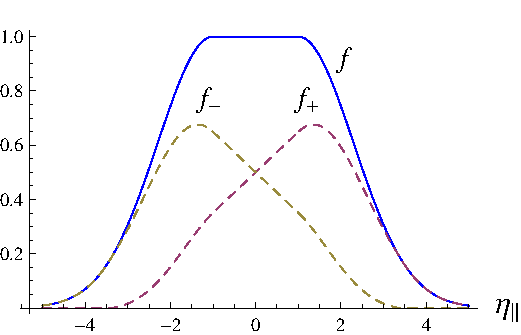
\includegraphics[width=.75\linewidth]{figs/chapter_fbcorr/cartoon_fb.pdf}
\caption{Cartoon showing particle production as a function of $\eta$. $f_+$ and $f_-$ correspond to the forward and backward emission functions respectively.}
\label{fig:fbcorr_cartoon_fb}
\end{figure}

On the other hand, short-range correlations can also be generated dynamically including resonance decay, jet fragmentation, and Bose-Einstein correlations. These correlations are typically localized over a smaller range of the $\eta$ and can be sensitive to final state effects. We will discuss the influences of short-range correlations in the ATLAS data analysis (see Section~\ref{sec:fb_atlas_data}).



\subsubsection{Previous studies and their limitations}

Most previous studies of the longitudinal multiplicity correlation are limited to two rapidity windows symmetric around the center-of-mass of the collision, commonly known as the forward-backward (FB) correlations~\cite{Bialas:2010zb}. The correlation strength is defined by the dependence of the average charged particle multiplicity in the backward hemisphere, $\lr{N_b}$, on the event multiplicity in the forward hemisphere, $N_f$, such that $\lr{N_b} = a + b N_f$, where $a$ is a constant and $b$ measures the correlation strength:
\begin{equation}
b = \frac{\lr{N_f N_b} - \lr{N_f}\lr{N_b}}{\lr{N_f^2} - \lr{N_f}^2} = \frac{D_{bf}^2}{D_{ff}^2}
\end{equation}
where $D_{bf}^2$ (covariance) and $D_{ff}^2$ (variance) are the backward-forward and forward-forward dispersions, respectively~\cite{Abelev:2009ag}. Since $N_f$ and $N_b$ are taken from two symmetric $\eta$ windows at $(\eta, -\eta)$, $\Delta\eta$ is used to quantify the separation of two windows. Correlation strength and similar observables have been measured experimentally in $e^+ e^-$~\cite{Braunschweig:1989bp}, $pp$~\cite{Uhlig:1977dc, ATLAS:2012as, Adam:2015mya}, $p\bar{p}$~\cite{Ansorge:1988fg, Alexopoulos:1995ft} and $A+A$~\cite{Abelev:2009ag} collisions where significant FB asymmetric component has been identified.

Figure~\ref{fig:fbcorr_star_fb} shows the FB correlation strength $b$ as a function of $\Delta\eta$ for $pp$ and centrality selected Au+Au collisions. It is observed that the magnitude of the FB correlation strength decreases with the decrease in centrality. The FB correlation strength evolves from a nearly flat function for $0-10\%$ to a sharply decreasing function with $\Delta\eta$ for the $40-50\%$ and $50-80\%$ centrality bins. Figure~\ref{fig:fbcorr_star_fb} also shows that the dependence of the FB correlation strength with $\Delta\eta$ is quite different in central Au+Au compared to $pp$ collisions.

\begin{figure}[H]
\centering
\includegraphics[width=.7\linewidth]{figs/chapter_fbcorr/star_fb.pdf}
\caption{(b) FB correlation strength for $10-20$, $20-30$, $30-40$, $40-50$ and $50-80\%$ Au+Au and (c) for $pp$ collisions as function of $\Delta\eta$ at $\sqrt{s_\text{NN}}=200$ GeV. The error bars represent the systematic point-to-point error. The boxes show the correlated systematic errors. This figure is taken from Ref.~\cite{Abelev:2009ag}.}
\label{fig:fbcorr_star_fb}
\end{figure}

However, there are few puzzles associated with these measurements, e.g., why correlation strength is stronger in central collisions, where the wounded nucleon fluctuations are smaller? How the short-range correlations affect the results? These questions reflect the limitations of previous correlation strength measurements:
\begin{itemize}
\item Correlation strength $b$ only measures multiplicity correlations in symmetric $\eta$ windows, hence lack of important information such as correlation between mid-rapidity and forward-rapidity;
\item Correlation strength $b$ is diluted by the variance in the denominator. This might explain the observed centrality dependence of the signal: peripheral events have larger tracking efficiency and statistical fluctuation, which leads to smaller $b$;
\item Short-range correlations usually extend to $\Delta\eta \sim 1$, and observed $\Delta\eta$-dependence for $\Delta\eta < 1$ might be due to the residual short-range correlations.
\end{itemize}

Recently, to address all of the limitations above, the forward-backward multiplicity correlation studies are extended by decomposing $N(\eta)$ into Chebyshev polynomials~\cite{Bzdak:2012tp} or into principle components~\cite{Bhalerao:2014mua}, with each mode representing the different components of the measured FB correlation. In our studies, we further extend the existing method by proposing a single-particle method that obtains these shape components directly from each event, as well as a two-particle correlation method that gives the ensemble RMS average of these shape components. We apply the method to HIJING and AMPT models and successfully extract the different shape components of the multiplicity fluctuation. The first component is found to be found to be directly related to the long-range asymmetry of the fireball, while the higher-order components are more related to the short-range correlations. The extracted components are also found to be dampened by the final-state interactions. To suppress the short-range correlations, the newly proposed correlators are measured with same and opposite changed particles separately, and this suppression technique is applied to the ATLAS data, as well as the QCD-inspired models such as PYTHIA~\cite{Sjostrand:2007gs} and EPOS~\cite{Pierog:2013ria}, to reveal the longitudinal multiplicity fluctuations in $pp$, $p$+Pb and Pb+Pb collision systems.



\subsection{Methodology}

\subsubsection{Observables}

\paragraph{Single-particle method}

Following previous notations, in a single event, the number of charged particles (multiplicity) in a given $\eta$ window is denoted as $N(\eta)$. To get rid of the average multiplicity, we define a normalized quantity $\rho(\eta)$:
\begin{equation}
\rho(\eta) \equiv \frac{N(\eta)}{\lr{N(\eta)}},
\end{equation}
where $\lr{N(\eta)}$ is the average distribution for a given event-multiplicity class. Legendre polynomials $P_n(x)$:
\begin{equation}
\begin{split}
P_0(x) &= 1 \\
P_1(x) &= x \\
P_2(x) &= \frac{1}{2}(3x^2 - 1)
\end{split}
\end{equation}
are used to quantify the shape of longitudinal multiplicity fluctuation. The particle density $\rho(\eta)$ in the interval $[-Y, Y]$ is then written in terms of Legendre polynomials:
\begin{equation}
\begin{split}
\rho(\eta) &\propto 1 + \sum a_n T_n(\eta) \\
T_n(\eta) &\equiv \sqrt{\frac{2n+1}{3}} Y P_n(\frac{\eta}{Y})
\end{split}
\end{equation}
where $a_n$ is the coefficient to be measured and the scaling factor $\sqrt{\frac{2n+1}{3}}$ is chosen such that $T_1(\eta)=\eta$.



\paragraph{Two-particle correlation method}

Single particle density $\rho(\eta)$ cannot be measured as an average over many similar events, due to $\lr{\rho(\eta)} = 1$. Thus the two-particle correlation function in $\eta$ is defined as:
\begin{equation}
C(\eta_1, \eta_2) \equiv \frac{\lr{N(\eta_1)N(\eta_2)}}{\lr{N(\eta_1)}\lr{N(\eta_2)}} = \lr{\rho(\eta_1)\rho(\eta_2)},
\end{equation}
where again the $N(\eta)$ is the multiplicity density distribution in a single event and $\lr{N(\eta)}$ is the average distribution for a given event-multiplicity class. The correlation function is directly related to a single-particle quantity $\rho(\eta)$, which characterizes the fluctuation of multiplicity in a single event relative to the average shape of the event class.

Compared with the correlation strength $b$, $C(\eta_1, \eta_2)$ has two advantages:
\begin{itemize}
\item $\eta_1$ and $\eta_2$ are not necessarily symmetric about zero, which makes $C(\eta_1, \eta_2)$ measures all possible correlated pairs in the full $\eta$ ranges $[-Y, Y]$;
\item The denominator of $C(\eta_1, \eta_2)$ is no longer a variance, thus tracking efficiency and statistical fluctuations have no influences on this new observable. 
\end{itemize}

In the single particle method, by construction, $\lr{a_n} = 0$. In the two-particle correlation method, we are going to measure $\lr{a_n a_m}$. Plug the $\rho(\eta)$ into the definition of $C(\eta_1, \eta_2)$ and we have:
\begin{equation}
C(\eta_1, \eta_2) = 1 + \sum \lr{a_n a_m} T_n(\eta_1) T_m(\eta_2)
\end{equation}
where $\lr{a_n a_m} \neq 0$, and this is one of the reasons why two particle correlation method is introduced. The shapes of the first two bases $T_n(\eta_1)T_m(\eta_2)$ are shown in Figure~\ref{fig:fbcorr_Legendre_base_2D}.

\begin{figure}[H]
\centering
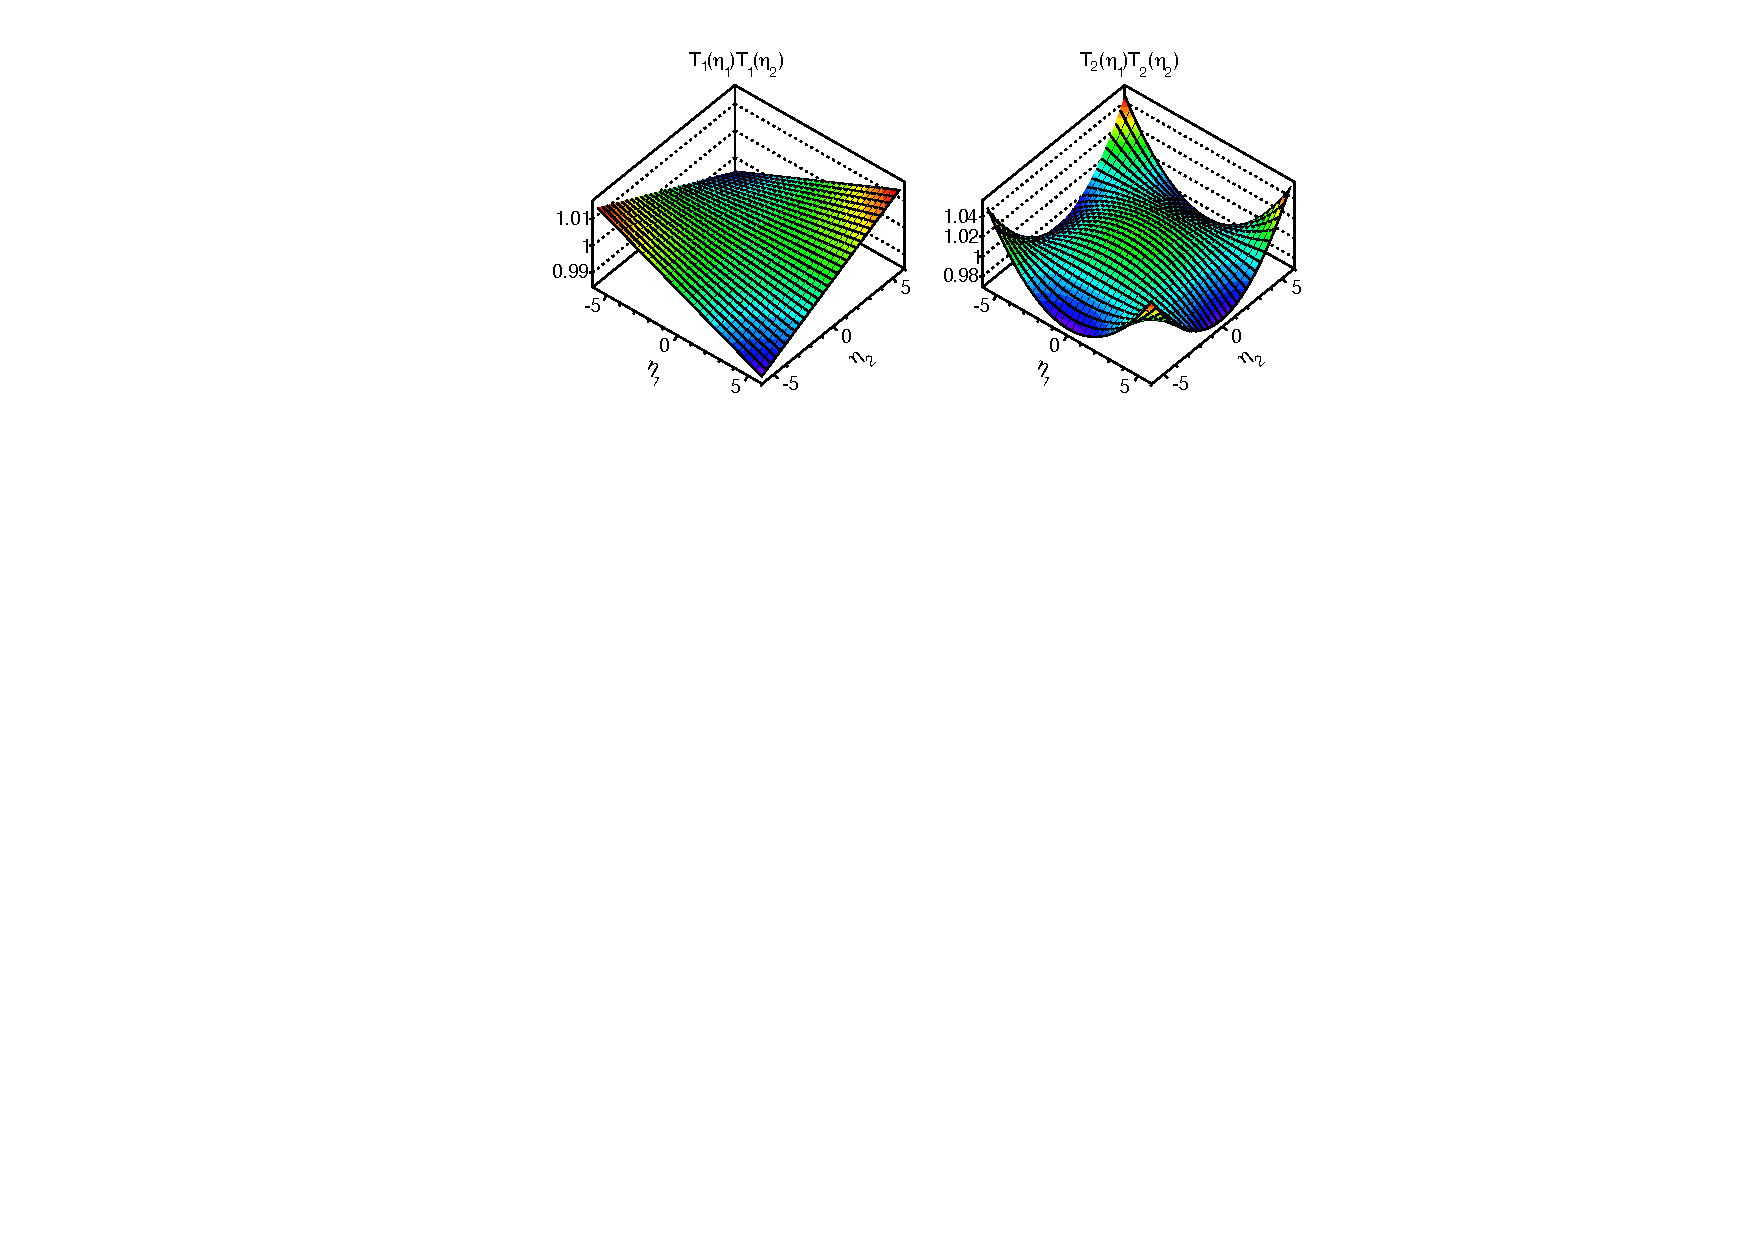
\includegraphics[width=.95\linewidth]{figs/chapter_fbcorr/Legendre_base_2D.pdf}
\caption{The shape of the first two bases associated with $\lr{a_n a_m}$ in the two-particle correlation function. They are plotted assuming $\lr{a_n a_m}=0.01$.}
\label{fig:fbcorr_Legendre_base_2D}
\end{figure}

Using the orthogonal relations of the Legendre polynomials:
\begin{equation}
\begin{split}
\int_{-Y}^Y T_n(\eta) d\eta &= 0 \\
\int_{-Y}^Y T_n(\eta) T_m(\eta) d\eta &= \frac{2Y^2}{3}\delta_{nm}
\end{split}
\end{equation}
where factor $\frac{2Y^2}{3}$ remains because of the scaling factor $\sqrt{\frac{2n+1}{3}}$ in the definition of $T_n(\eta)$, one could calculate the two-particle Legendre coefficients directly:
\begin{equation}
\lr{a_n a_m} = (\frac{3}{2Y^3})^2 \int_{-Y}^Y C(\eta_1, \eta_2) T_n(\eta_1) T_m(\eta_2) d\eta_1 d\eta_2
\end{equation}
One of the reasons we prefer Legendre polynomials to Chebyshev polynomials~\cite{Bzdak:2012tp} is that in the orthogonal relation of Legendre polynomials, there is no additional weight as a function of $\eta$. The two-particle correlation method measures, in effect, the RMS values of the EbyE $a_n$, $\sqrt{\lr{a_n^2}}$, or the cross correlation between $a_n$ and $a_m$, $\lr{a_n a_m}$. The correlation functions satisfy the symmetric condition $C(\eta_1, \eta_2) = C(\eta_2, \eta_1)$.

Among all the terms of $\lr{a_n a_m}$, terms such as $\lr{a_0 a_n}$ involve the correlation between shape fluctuation $a_n$ and the overall multiplicity fluctuation $a_0$. Provided all deviations from one are small, the terms involving $\lr{a_0 a_n}$ can be removed. We define normalized two-particle correlation $C_N(\eta_1, \eta_2)$:
\begin{equation}
\begin{split}
C_N(\eta_1, \eta_2) &= \frac{C(\eta_1, \eta_2)}{C_p(\eta_1) C_p(\eta_2)} \\
C_p(\eta_1) &= \frac{\int_{-Y}^Y C(\eta_1, \eta_2) d\eta_2}{2Y} \\
C_p(\eta_2) &= \frac{\int_{-Y}^Y C(\eta_1, \eta_2) d\eta_1}{2Y}
\end{split}
\end{equation}
where the quantities $C_p(\eta_1)$ and $C_p(\eta_2)$ are referred to as the single-particle modes. The $\lr{a_0 a_0}$ term can be removed by renormalizing average value in the $\eta_1$, $\eta_2$ phase space to be one.



\subsubsection{Removal of short-range correlation}

\paragraph{Outline}

The aim of our studies is to measure and parametrize the long-range correlation (LRC), which requires the separation and subtraction of the short-range correlation (SRC). The separation of SRC and LRC is quite involved and so is briefly summarized here, with details left to the sections below.

The core of the separation method is to exploit the difference between the correlations for opposite-charge and same-charge pairs, $C^{+-}(\eta_1, \eta_2)$ and $C^{\pm\pm}(\eta_1, \eta_2)$, respectively. The SRC component centered around $\eta_- \equiv \eta_1 - \eta_2 \sim 0$ is found to be much stronger for opposite-charge pairs, primarily due to local charge conservation, while the LRC and single-particle modes are expected to be independent of the charge combination. With this assumption, the ratio $R(\eta_1, \eta_2)$ can be approximated by:
\begin{equation}
\begin{split}
R(\eta_1, \eta_2) &= \frac{C^{+-}(\eta_1, \eta_2)}{C^{\pm\pm}(\eta_1, \eta_2)} \\
&= \frac{1 + C_\text{LRC}^{+-}(\eta_1, \eta_2) + \dSo(\eta_1, \eta_2)}{1 + C_\text{LRC}^{\pm\pm}(\eta_1, \eta_2) + \dSs(\eta_1, \eta_2)} \\
&\approx 1 + \dSo(\eta_1, \eta_2) - \dSs(\eta_1, \eta_2)
\end{split}
\end{equation}
where $C_\text{LRC}(\eta_1, \eta_2)$ and $\delta_\text{SRC}(\eta_1, \eta_2)$ represent the correlations for LRC and SRC separately. The results can be approximated because both LRC and SRC are significantly smaller than one.

Our studies further assume that the dependence of $\delta_\text{SRC}$ on $\eta_-$ and $\eta_+ \equiv \eta_1 + \eta_2$ factorizes and that the dependence on $\eta_+$ is independent of the charge combinations
\begin{equation}
\begin{split}
\dSo(\eta_+, \eta_-) &= f(\eta_+)g^{+-}(\eta_-) \\
\dSs(\eta_+, \eta_-) &= f(\eta_+) g^{\pm\pm}(\eta_-)
\end{split}
\end{equation}
where $g^{+-}(\eta_-)$ and $g^{\pm\pm}(\eta_-)$ are allowed to differ in both shape and magnitude. The validity of these various assumptions is confirmed in the data from the extracted $\delta_{SRC}^{+-}(\eta_+, \eta_-)$ and $\delta_{SRC}^{\pm\pm}(\eta_+, \eta_-)$ after applying the separation procedure. With these assumptions, $f(\eta_+)$ can be determined from $R$ by suitable integration over $\eta_-$, as described in Section~\ref{sec:probing_the_src_via_the_same_charge_and_opposite_charge_correlations}.

To complete the determination of $\dSs$, the quantity $g^{\pm\pm}$ is determined and parameterized from suitable projections of $C_N^{\pm\pm}(\eta_+, \eta_-)$ in the $\eta_-$ direction, as described in Section~\ref{sec:separation_of_the_src_and_the_lrc}. The use of $C_N^{\pm\pm}$ rather than $C^{\pm\pm}$ is because the former does not contain the single-particle modes. The procedure to obtain a correlation function with the SRC subtracted is also described in Section~\ref{sec:separation_of_the_src_and_the_lrc}. With $\dSs$ determined, $\dSo$ can be obtained directly. The $\dSs$ and $\dSo$ are then averaged to obtain the SRC for all charge combinations, $\delta_\text{SRC}$.

This SRC estimation technique is mainly applied to the ATLAS data, and briefly tested on PYTHIA and EPOS MC samples. For demonstration purpose, Pb+Pb and $p$+Pb collision systems are discussed in the section.



\paragraph{Probing the SRC via the same-charge and opposite-charge correlations}
\label{sec:probing_the_src_via_the_same_charge_and_opposite_charge_correlations}

Figure~\ref{fig:fbcorr_ATLAS_SRCremoval_PbPb} shows separately the correlation functions for same-charge pairs and opposite-charge pairs from Pb+Pb collisions with $200 \le \Nchrec < 220$. The ratio of the two, $R(\eta_1, \eta_2)$, is shown in the top right panel. The correlation functions show a narrow ridge-like shape along $\eta_1 \approx \eta_2$ or $\eta_- \approx 0$, and a falloff towards the corners at $\eta_1 = -\eta_2 \approx \pm 2.4$. The magnitude of the ridge for the opposite-charge pairs is stronger than that for the same-charge pairs, which is characteristic of the influence from SRC from jet fragmentation or resonance decays. In regions away from the SRC, i.e., large values of $|\eta_-|$, the ratio approaches unity, suggesting that the magnitude of the LRC is independent of the charge combinations. To quantify the shape of the SRC in the ratio along $\eta_+$, $R$ is expressed in terms of $\eta_+$ and $\eta_-$, $R(\eta_+, \eta_-)$, and the following quantity is calculated:
\begin{equation}
f(\eta_+) = \frac{\frac{1}{0.8} \int_{-0.4}^{0.4} R(\eta_+, \eta_-)d\eta_- - 1}{\frac{1}{0.8} \int_{-0.4}^{0.4} R(0, \eta_-)d\eta_- - 1}
\end{equation}
As shown in Figure~\ref{fig:fbcorr_ATLAS_SRCremoval_PbPb}, the quantity $f(\eta_+)$ is nearly constant in Pb+Pb collisions, implying that the SRC is consistent with being independent of $\eta_+$. To quantify the shape of the SRC along the $\eta_-$ direction, $R(\eta_+, \eta_-)$ is fitted to a Gaussian function in slices of $\eta_+$. The width, as shown in the bottom middle panel of Figure~\ref{fig:fbcorr_ATLAS_SRCremoval_PbPb}, is constant, which may suggest that the shape of the SRC in $\eta_-$ is the same for different $\eta_+$ slices.

\begin{figure}[H]
\centering
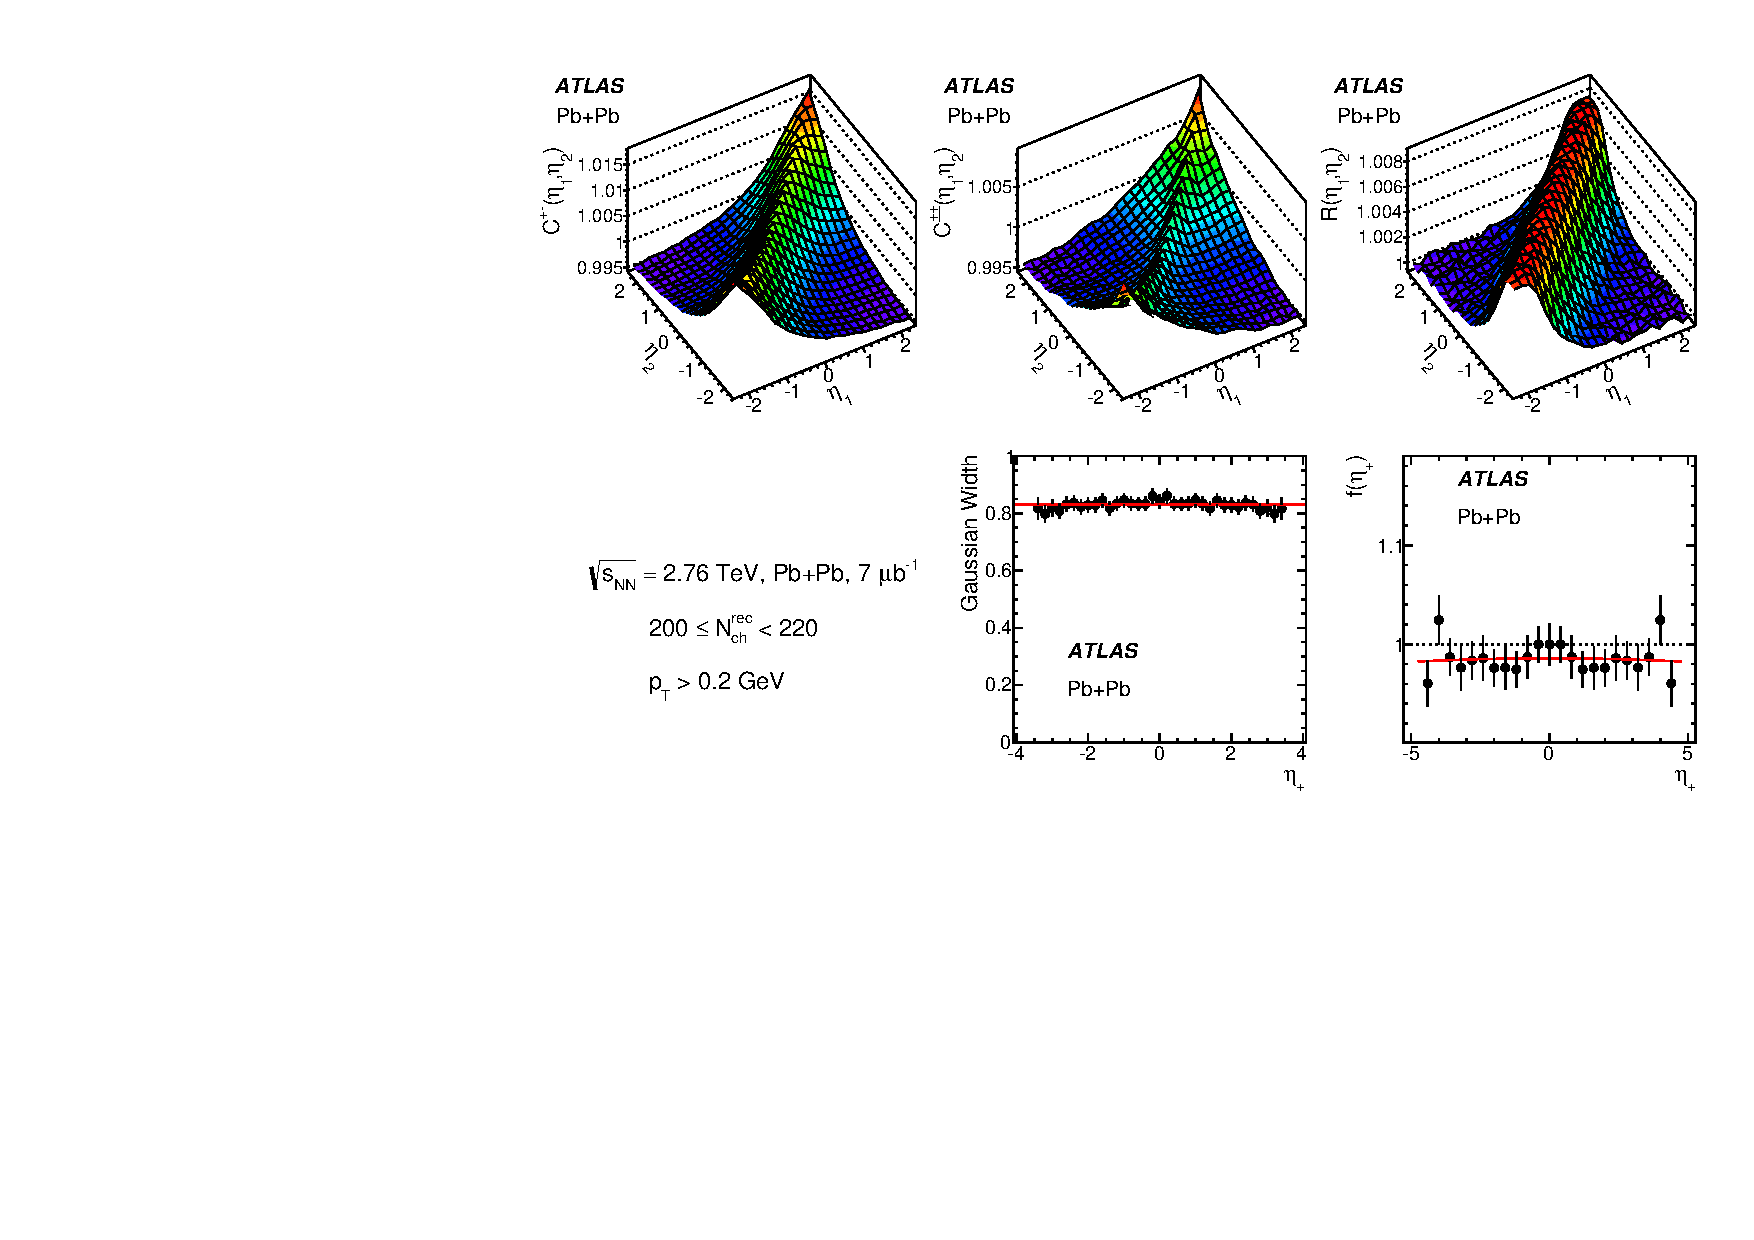
\includegraphics[width=.95\linewidth]{figs/chapter_fbcorr/ATLAS_SRCremoval_PbPb.pdf}
\caption{The correlation functions for opposite-charge pairs $C^{+-}(\eta_1, \eta_2)$ (top left), same-charge pairs $C^{\pm\pm}(\eta_1, \eta_2)$ (top middle) and the ratio $R(\eta_1, \eta_2)$ (top right) for Pb+Pb collisions with $200 \le \Nchrec < 220$. The width and magnitude of the short-range Gaussian peak of the ratio are shown in the lower middle and right panels. The error bars represent the statistical uncertainties, and the solid lines indicate a quadratic fit.}
\label{fig:fbcorr_ATLAS_SRCremoval_PbPb}
\end{figure}

Figure~\ref{fig:fbcorr_ATLAS_SRCremoval_pPb} shows the correlation function in $p$+Pb collisions with multiplicity similar to the Pb+Pb data in Figure~\ref{fig:fbcorr_ATLAS_SRCremoval_PbPb}. The correlation function shows a significant asymmetry between the proton-going side (positive $\eta_+$) and lead-going side (negative $\eta_+$). However, much of this asymmetry appears to be confined to a small $|\eta_-|$ region where the SRC dominates. The magnitude of the SRC, estimated by $f(\eta_+)$ shown in the bottom-right panel, increases by about $50\%$ from the lead-going side (negative $\eta_+$) to the proton-going side (positive $\eta_+$), but the width of the SRC in $\eta_-$ is independent of $\eta_+$ as shown in the bottom-middle panel. In contrast, the LRC has no dependence on the charge combinations, since the value of $R$ approaches unity at large $|\eta_-|$.

\begin{figure}[H]
\centering
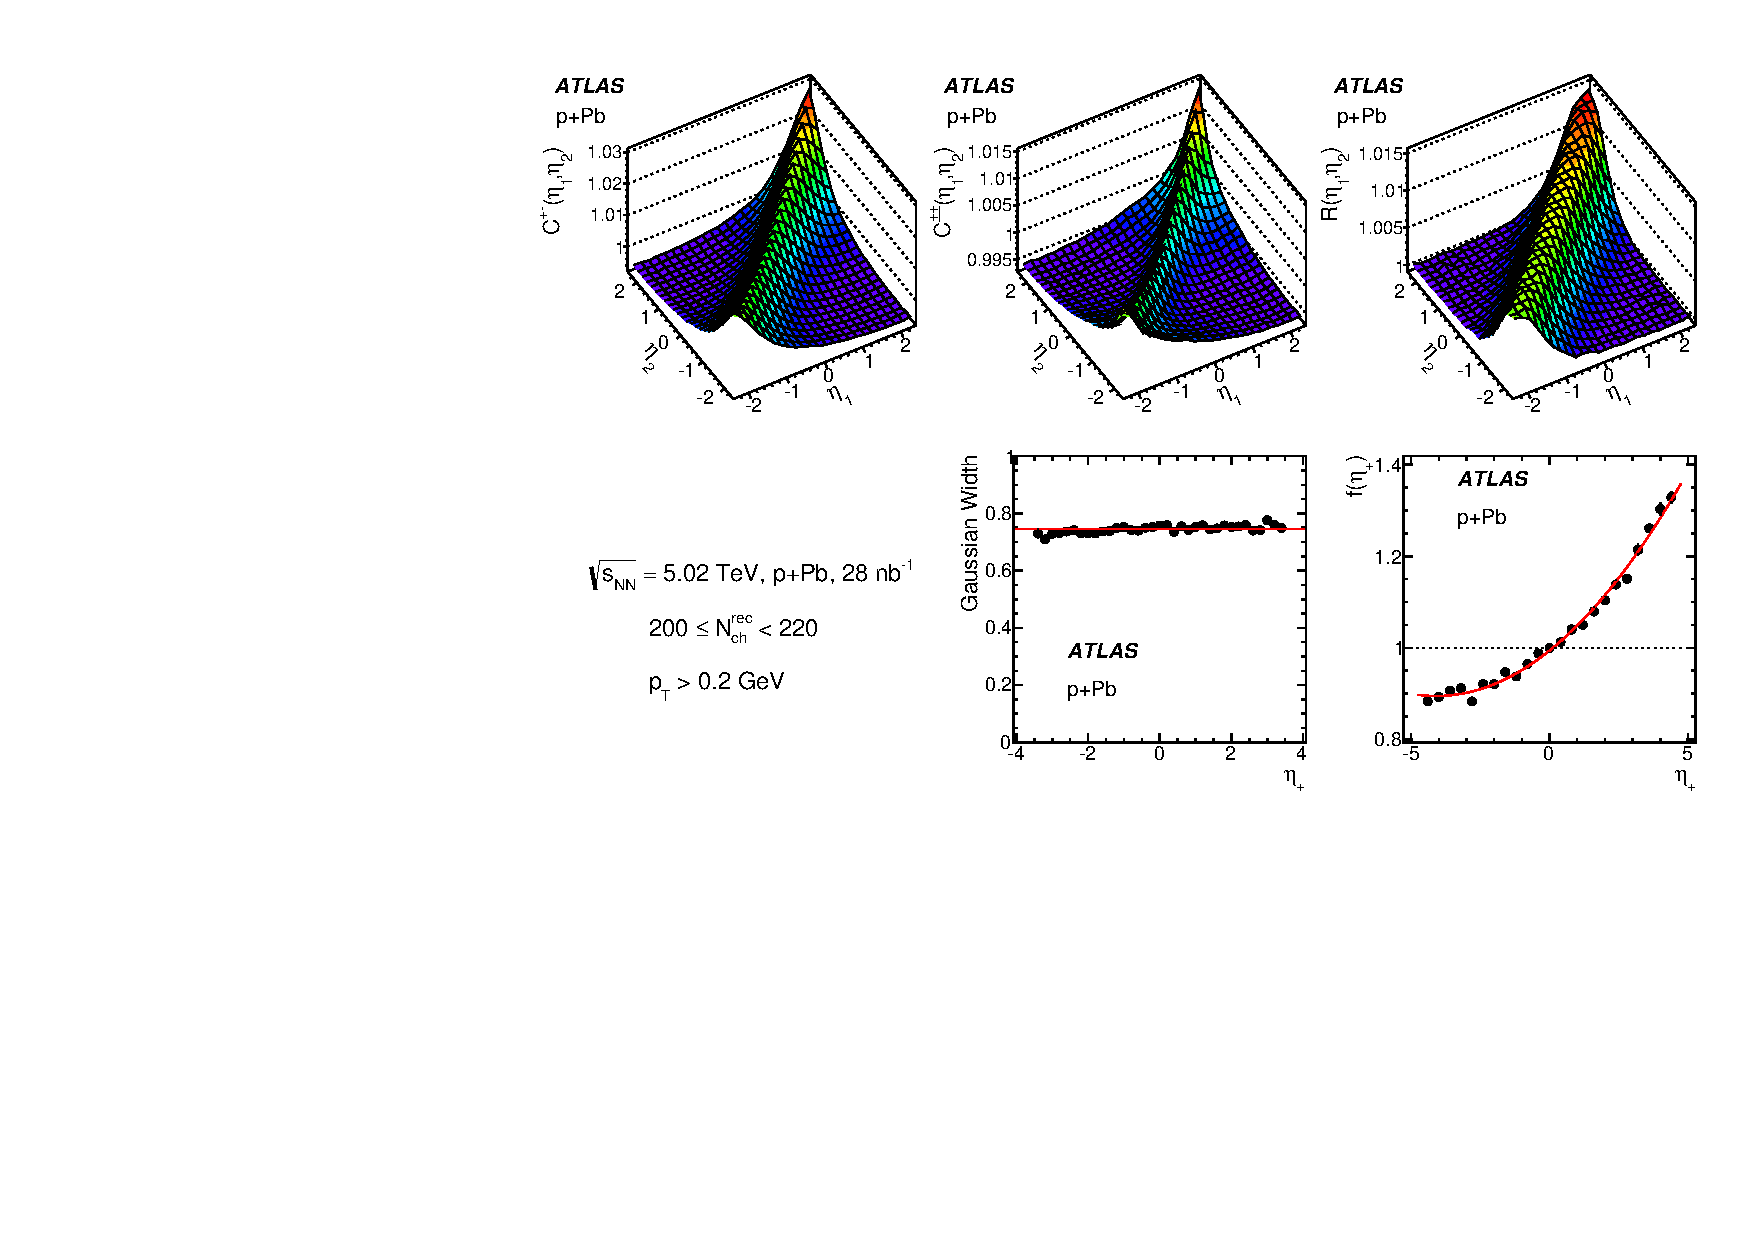
\includegraphics[width=.95\linewidth]{figs/chapter_fbcorr/ATLAS_SRCremoval_pPb.pdf}
\caption{The correlation functions for opposite-charge pairs $C^{+-}(\eta_1, \eta_2)$ (top left), same-charge pairs $C^{\pm\pm}(\eta_1, \eta_2)$ (top middle) and the ratio $R(\eta_1, \eta_2)$ (top right) for $p$+Pb collisions with $200 \le \Nchrec < 220$. The width and magnitude of the short-range Gaussian peak of the ratio are shown in the lower middle and right panels. The error bars represent the statistical uncertainties, and the solid lines indicate a quadratic fit.}
\label{fig:fbcorr_ATLAS_SRCremoval_pPb}
\end{figure}

Left panel of Figure~\ref{fig:fbcorr_ATLAS_SRCremoval_sysComp} shows the width in $\eta_-$ of the short-range component as a function of $\Nch$ in the three collision systems. The width is obtained as the Gaussian width of $R(\eta_+, \eta_-)$ in the $\eta_-$ direction, and then averaged over $\eta_+$ as the width is observed to be independent of $\eta_+$, as shown in Figure~\ref{fig:fbcorr_ATLAS_SRCremoval_PbPb} and~\ref{fig:fbcorr_ATLAS_SRCremoval_pPb}. This width reflects the extent of the short-range correlation in $\eta$, and it is observed to decrease with increasing $\Nch$ in all collision systems. At the same $\Nch$ value, the width is smallest in $pp$ collisions and largest in Pb+Pb collisions. In the right panel of Figure~\ref{fig:fbcorr_ATLAS_SRCremoval_sysComp}, the width of the short-range component from $pp$ data is compared with PYTHIA 8 based on the A2 tune~\cite{ATL-PHYS-PUB-2011-014} and EPOS based on the LHC tune~\cite{Pierog:2013ria}. The width of is underestimated by PYTHIA 2 A2 and overestimated by EPOS LHC.

\begin{figure}[H]
\centering
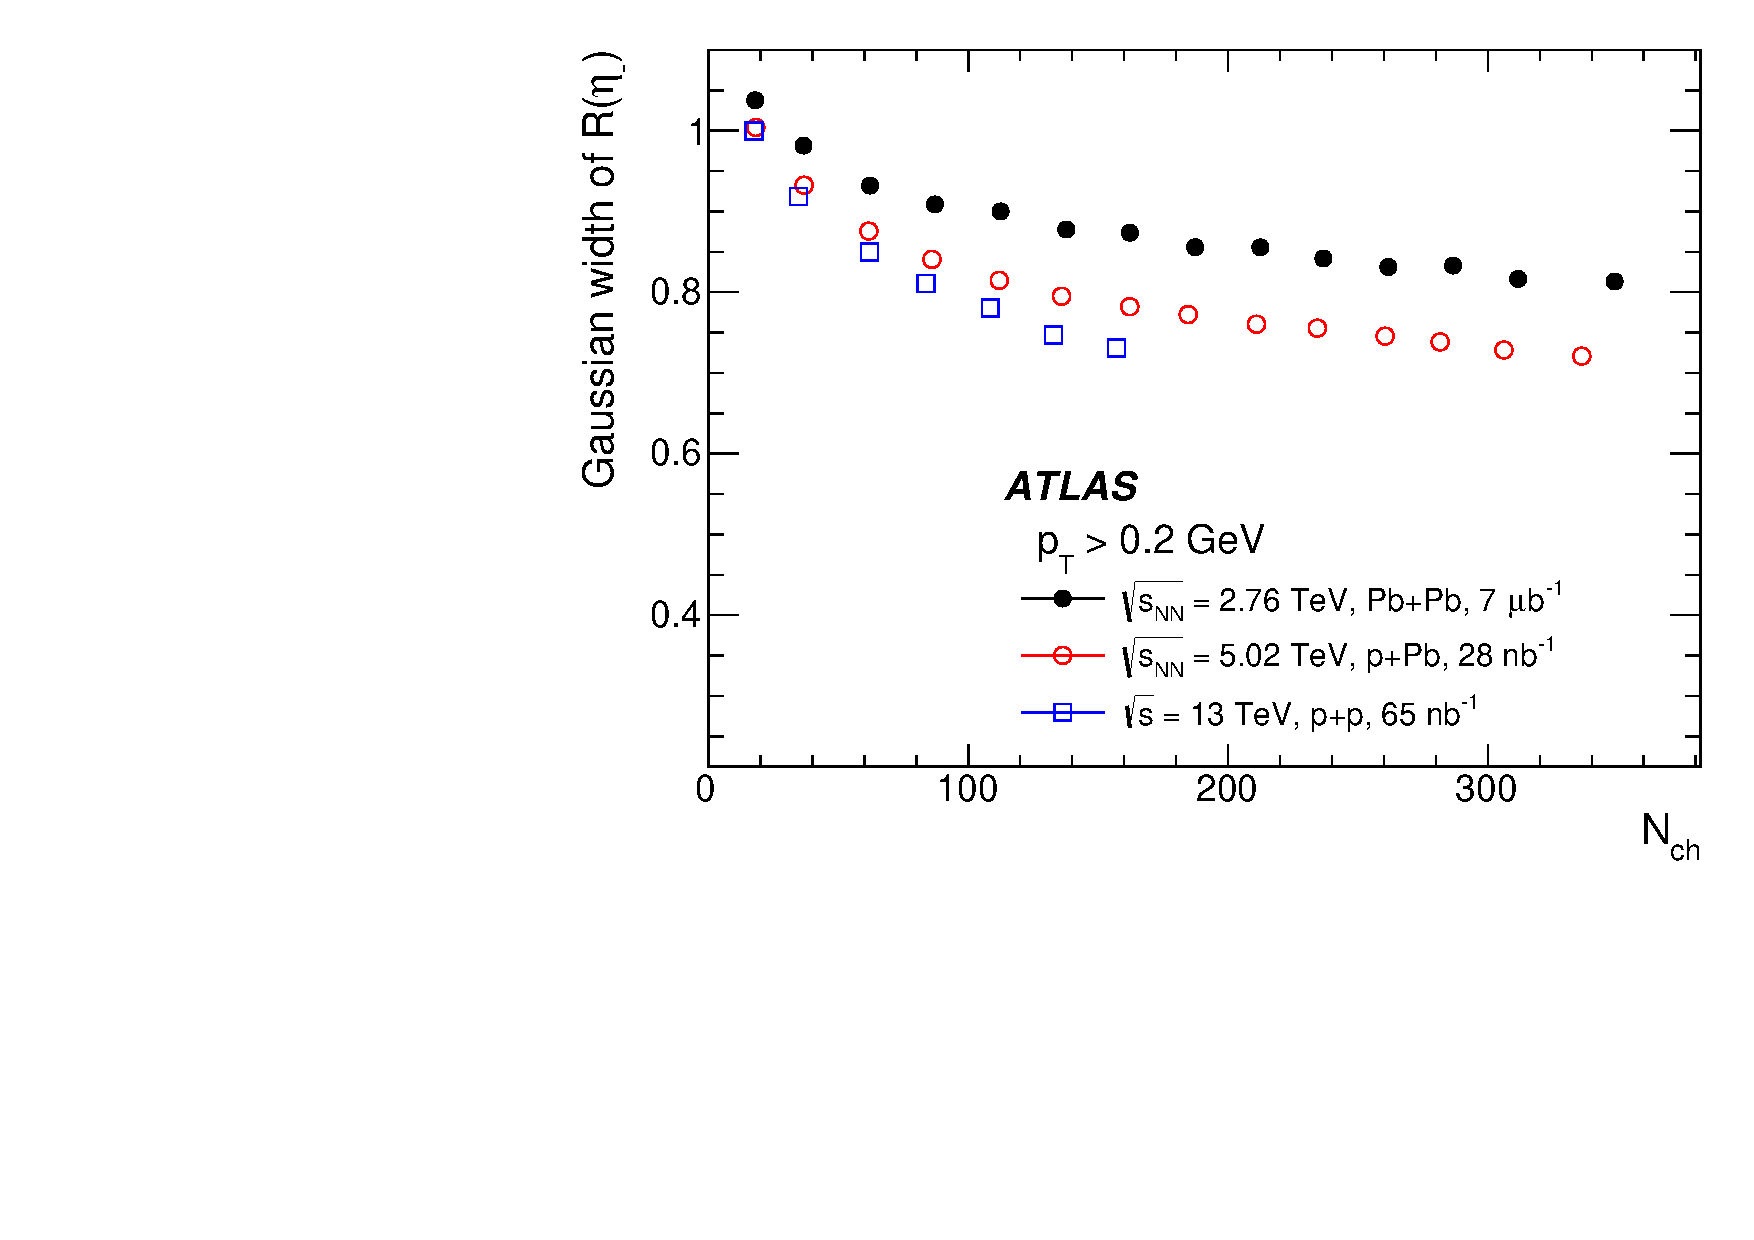
\includegraphics[width=.475\linewidth]{figs/chapter_fbcorr/ATLAS_SRCremoval_sysComp.pdf}
\includegraphics[width=.475\linewidth]{figs/chapter_fbcorr/ATLAS_SRCremoval_modelComp.pdf}
\caption{The width of the short-range component in $R(\eta_+, \eta_-)$ along the $\eta_-$ direction as a function of $\Nch$: in three collision systems (left), compared between data and two models.}
\label{fig:fbcorr_ATLAS_SRCremoval_sysComp}
\end{figure}



\paragraph{Separation of the SRC and the LRC}
\label{sec:separation_of_the_src_and_the_lrc}

As discussed before, the ratio of the correlation function between opposite-charge and same-charge pairs $R(\eta_+, \eta_-)$ is the key to the separation of the SRC and LRC. Following above equations, this ratio can be approximated by:
\begin{equation}
\begin{split}
R(\eta_+, \eta_-) &\approx 1 + f(\eta_+) [g^{+-}(\eta_-) - g^{\pm\pm}(\eta_-)] \\
\dSo &= f(\eta_+) g^{+-}(\eta_-) \\
\dSs &= f(\eta_+) g^{\pm\pm}(\eta_-)
\end{split}
\end{equation}
where $f(\eta_+)$ describes the magnitude along $\eta_+$ and can be calculated from $R(\eta_+, \eta_-)$. The functions $g^{+-}$ and $g^{\pm\pm}$ describe the SRC along the $\eta_-$ direction for the two charge combinations, which differ in both magnitude and shape.

In order to estimate the $g^{\pm\pm}(\eta_-)$ function for same-charge pairs, the $C_N(\eta_+, \eta_-)$ distributions for same-charge pairs are projection into one-dimensional $\eta_-$ distributions over a narrow slice $|\eta_+|<0.4$. The distributions are denoted by $C_N(\eta_-)$. They are shown, after a small iterative correction discussed below, in the second column of Figure~\ref{fig:fbcorr_ATLAS_SRCremoval_fit} for the same-charge pairs in Pb+Pb and $p$+Pb collisions. The SRC appears as a narrow peak on top of a distribution that has an approximately quadratic shape. Therefore, a quadratic fit is applied to the data in the region of $|\eta_-|>1.5$, and the difference between the data and fit in the $|\eta_-|<2$ region is taken as the estimated SRC component or the $g^{\pm\pm}(\eta_-)$ function, which is assumed to be zero for $|\eta_-|>2$. This range ($|\eta_-|>1.5$) is about twice the width of the short-range peak in the $R(\eta_+, \eta_-)$ distribution along the $\eta_-$ distribution. This width is observed to decrease from 1.0 to 0.7 as a function of $\Nchrec$ in the $p$+Pb collisions, and is slightly broader in Pb+Pb collisions and slightly narrower in $pp$ collisions at the same $\Nchrec$. The range of the fit is varied from $|\eta_-|>1.0$ to $|\eta_-|>2.0$ to check the sensitivity of the SRC estimation, and the variation is included in the final systematic uncertainties. Furthermore, this study is also repeated for $C_N(\eta_-)$ obtained in several other $\eta_+$ slices within $|\eta_+|<1.2$, and consistent results are obtained. Once the distribution $g^{\pm\pm}(\eta_-)$ for same-charge pairs is obtained from the fit, it is multiplied by the $f(\eta_+)$ function calculated from $R(\eta_+, \eta_-)$ to obtain the $\delta(\eta_1, \eta_2)$ in the full phase space. Subtracting this distribution from the $C_N(\eta_1, \eta_2)$ distribution, one obtains the initial estimate of the correlation function containing mostly the LRC component.

\begin{figure}[H]
\centering
\includegraphics[width=.95\linewidth]{figs/chapter_fbcorr/ATLAS_SRCremoval_fit.pdf}
\caption{The separation of correlation functions for same-charge pairs (first column) into the SRC (third column) and the LRC (last column) for Pb+Pb (top row) and $p$+Pb (bottom row) collisions with $200 \le \Nchrec < 220$. The second column shows the result of the quadratic fit over the $|\eta_-|>1.5$ range of the one-dimensional correlation function projected over the $|\eta_+|<0.4$ slice, which is used to estimate the SRC component. The error bars represent the statistical uncertainties.}
\label{fig:fbcorr_ATLAS_SRCremoval_fit}
\end{figure}



\paragraph{Iterative correction for single-particle mode}

The LRC obtained via this procedure is still affected by a small bias from the SRC via the normalization procedure of $C_N(\eta_1, \eta_2)$. This bias appears because the $\delta_\text{SRC}(\eta_1, \eta_2)$ contribution is removed from the numerator but is still included in the denominator via $C_p(\eta)$. This contribution is not uniform in $\eta$: If the first particle is near mid-rapidity $\eta_1 \approx 0$ then all pairs in $\delta_\text{SRC}(\eta_1, \eta_2)$ contribute to $C_p(\eta_1)$, whereas if the first particle is near the edge of the acceptance $\eta_1 \approx \pm Y$ then only half of the pairs in $\delta_\text{SRC}(\eta_1, \eta_2)$ contribute to $C_p(\eta_1)$. The acceptance bias in $C_p$ is removed via a simple iterative procedure: First, the $\delta_\text{SRC}$ contribution determined from the above procedure is used to eliminate the SRC contribution to the single-particle mode:
\begin{equation}
\begin{split}
C_p^\text{sub}(\eta_1) &= \frac{\int_{-Y}^Y [C(\eta_1, \eta_2) - \delta_\text{SRC}(\eta_1, \eta_2)] d\eta_2}{2Y} \\
C_p^\text{sub}(\eta_2) &= \frac{\int_{-Y}^Y [C(\eta_1, \eta_2) - \delta_\text{SRC}(\eta_1, \eta_2)] d\eta_1}{2Y}.
\end{split}
\end{equation}
The $C_p^\text{sub}(\eta_1)$ and $C_p^\text{sub}(\eta_2)$ are then used to redefine the $C_N$ function:
\begin{equation}
C_N^{'}(\eta_1, \eta_2) = \frac{C(\eta_1, \eta_2)}{C_p^\text{sub}(\eta_1) C_p^\text{sub}(\eta_2)}.
\end{equation}
This distribution, which is very close to the distribution before correction, is shown in the second column of Figure~\ref{fig:fbcorr_ATLAS_SRCremoval_fit} for projection over a narrow slice $|\eta_+|<0.4$. The estimation of $\delta_\text{SRC}(\eta_1, \eta_2)$ is repeated using the previously described procedure for the $C_N^{'}(\eta_1, \eta_2)$, and the extracted distribution is shown in the third column of Figure~\ref{fig:fbcorr_ATLAS_SRCremoval_fit}. Subtracting this distribution from $C_N^{'}(\eta_1, \eta_2)$, one obtains the correlation function containing only the LRC component. The resulting correlation function, denoted $C_N^\text{sub}(\eta_1, \eta_2)$, is shown in the last column of Figure~\ref{fig:fbcorr_ATLAS_SRCremoval_fit}.

The results presented in this study are obtained using the iterative procedure discussed above. In most cases, the results obtained from the iterative procedure are consistent with the one obtained without iteration. In $p$+Pb and Pb+Pb collisions, where the SRC component is small, the difference between the two methods is found to be less than $2\%$. In $pp$ collisions with $\Nchrec>100$, the difference between the two methods reaches $4\%$ where the SRC is large and therefore the bias correction is more important.

In principle, the same analysis procedure can be applied to opposite-charge and all-charge pairs. However, due to the much large SRC, the extracted LRC for opposite-charge pairs has larger uncertainties. Instead, the SRC for opposite-charge pairs is obtained directly:
\begin{equation}
\delta_\text{SRC}^{+-}(\eta_1, \eta_2) = R(\eta_1, \eta_2) - 1 + \delta_\text{SRC}^{\pm\pm}(\eta_1, \eta_2)
\end{equation}
The SRC for all-charge pairs is calculated as the average of $\delta_\text{SRC}^{\pm\pm}$ and $\delta_\text{SRC}^{+-}$ weighted by the number of same-charge and opposite-charge pairs. The LRC is then obtained by subtracting the SRC from the modified $C_N(\eta_1, \eta_2)$ using the same procedure as that for the same-charge pairs.

For $pp$ collisions, the pseudorapidity correlations are also compared with the PYTHIA 8 A2 and EPOS LHC event generators mentioned above. The analysis procedure used on the data is repeated for the two models in order to extract the SRC and LRC components. The correlation is carried our on the generated, as opposed to the reconstructed, charged particles.



\subsubsection{Other independent observables}
\label{sec:fb_other_observables}

In the azimuthal correlation analysis, the azimuthal structure of the correlation function is characterized by harmonic coefficients $v_n$ obtained via a Fourier decomposition~\cite{ATLAS:2012at, Aamodt:2011by}. A similar approach can be applied for pseudorapidity correlations. As discussed above, the correlation functions are expanded into Legendre polynomial functions, and the two-particle Legendre coefficients $\lr{a_n a_m}$ are calculated directly from the correlation. The two-particle correlation method measures, in effect, the RMS values of the EbyE $a_n$, and the final results for the coefficients are presented in terms of $\sqrt{|a_n a_m|}$. As a consequence of the condition for a symmetric collision system, the odd and even coefficients should be uncorrelated in $pp$ and Pb+Pb collisions:
\begin{equation}
\lr{a_n a_{n+1}} = 0.
\end{equation}
However, even in $p$+Pb collisions, the correlation function after SRC removal, $C_M^\text{sub}(\eta_1, \eta_2)$, is observed to be nearly symmetric between $\eta$ and $-\eta$ (right column of Figure~\ref{fig:fbcorr_ATLAS_SRCremoval_fit}), and hence the $\lr{a_n a_{n+1}}$ values are very small and considered to be negligible in this study.

The shape of the first two Legendre bases in 2D are shown in Figure~\ref{fig:fbcorr_Legendre_base_2D}. The first basis function has the shape of $\eta_1 \times \eta_2$ and is directly sensitive to the FB asymmetry of the EbyE fluctuation. The second basis function has a quadratic shape in the $\eta_1$ and $\eta_2$ directions and is sensitive to the EbyE fluctuation in the width of the $N(\eta)$ distribution. It is shown in Section~\ref{sec:fb_atlas_data} that the data require only the first term, in which case the shape of the correlation function can be approximated by
\begin{equation}
C_N^\text{sub}(\eta_1, \eta_2) \approx 1 + \lr{a_1^2}\eta_1\eta_2 = 1 + \frac{\lr{a_1^2}}{4}(\eta_+^2 - \eta_-^2).
\end{equation}
Therefore, a quadratic shape is expected along the two diagonal directions $\eta_+$ and $\eta_-$ of the correlation function, and the $\sqrt{\lr{a_1^2}}$ coefficient can be calculated by a simple quadratic fit of $C_N^\text{sub}$ in narrow slices of $\eta_-$ and $\eta_+$.

Alternatively, $\sqrt{\lr{a_1^2}}$ can also be estimated from a correlator constructed from a simple ratio:
\begin{equation}
\begin{split}
r_N^\text{sub}&(\eta, \eta_\text{ref}) \\
&=\left\{\begin{array}{l} \frac{C_N^\text{sub}(-\eta, \eta_\text{ref})}{C_N^\text{sub}(\eta, \eta_\text{ref})}, \eta_\text{ref}>0, \\ \frac{C_N^\text{sub}(\eta, -\eta_\text{ref})}{C_N^\text{sub}(-\eta, -\eta_\text{ref})}, \eta_\text{ref}<0, \end{array}\right. \\
&\approx 1 - 2 \lr{a_1^2} \eta \eta_\text{ref}
\end{split}
\end{equation}
where $\eta_\text{ref}$ is a narrow interval of 0.2. This correlator has the advantage that most of the single-particle modes are even functions in $\eta$, so they cancel in the ratios. Therefore, this correlator provides a robust consistency check of any potential bias introduced by the normalization procedure to remove the single-particle modes. A similar quantity can also be calculated for $C_N(\eta_1, \eta_2)$, denoted by $r_N(\eta, \eta_\text{ref})$.

In summary, this study uses the following four different methods to estimate $\sqrt{\lr{a_1^2}}$:
\begin{itemize}
\item Legendre decomposition of the 2D correlation function $C_N^\text{sub}(\eta_+, \eta_-)$;
\item Quadratic fit of $C_N^\text{sub}(\eta_-)$ in a narrow slice of $\eta_+$, which gives $\sqrt{\lr{a_1^2}}$ as a function of $\eta_-$;
\item Quadratic fit of $C_N^\text{sub}(\eta_+)$ in a narrow slice of $\eta_-$, which gives $\sqrt{\lr{a_1^2}}$ as a function of $\eta_+$;
\item Linear fit of $r_N^\text{sub}(\eta)$ in a narrow slice of $\eta_\text{ref}$, which gives $\sqrt{\lr{a_1^2}}$ as a function of $\eta_\text{ref}$.
\end{itemize}
The last three fitting methods use the correlation function in limited and largely non-overlapping regions of the $\eta_1$ and $\eta_2$ phase space, and therefore are independent of each other and largely independent of the Legendre decomposition method. Moreover, if the correlation function is dominated by the $\lr{a_1^2}$ term, the results from all four methods should be consistent.



\subsection{Results}

\subsubsection{HIJING and AMPT models}
\label{sec:hijing_and_ampt_models}

\paragraph{Correlating single-particle $a_n$ with participants asymmetry}

The event-by-event observed single-particle $a_n^\text{obs}$ suffers from statistical fluctuations, which can be estimated by randomizing the $N(\eta)$ distribution in each event based on the profile of $\lr{N(\eta)}$ of that event class. The RMS of $a_n$ without the statistical fluctuations can be calculated as:
\begin{equation}
\lr{a_n^2} = \lr{(a_n^\text{obs})^2} - \lr{(a_n^\text{ran})^2}
\end{equation}
where $a_n^\text{ran}$ denotes the coefficient calculated from the randomized events described above.

Figure~\ref{fig:fbcorr_Model_an} compares the centrality dependence of the $a_1$, $a_2$ and $a_3$ in HIJING and AMPT models. The signal strength increases towards more peripheral collisions and the values from AMPT model are consistently smaller than those from HIJING in all centralities.

\begin{figure}[H]
\centering
\includegraphics[width=.95\linewidth]{figs/chapter_fbcorr/Model_an.pdf}
\caption{Centrality dependence of $a_1$ (left), $a_2$ (middle) and $a_3$ (right) for HIJING and AMPT events.}
\label{fig:fbcorr_Model_an}
\end{figure}

In order to find out whether the FB multiplicity fluctuation is related to the difference between $\Nf$ and $\Nb$, $a_n^\text{obs}$ is correlated directly with $A_\text{part}$, defined as
\begin{equation}
A_\text{part} = \frac{\Nf - \Nb}{\Nf + \Nb}
\end{equation}
The results for impact parameter $b=8$ fm from HIJING events are shown in Figure~\ref{fig:fbcorr_Model_an_Anpart} (results for AMPT events are similar). A strong positive correlation between $a_1^\text{obs}$ and $A_\text{part}$ is observed, suggesting that the FB asymmetry in the multiplicity distribution is indeed driven by the asymmetry in the number of participating nucleons in the two colliding nuclei. A weak correlation is also observed between $a_3^\text{obs}$ and $A_\text{part}$, suggesting that the FB asymmetry caused by $A_\text{part}$ contains a small nonlinear odd component. On the other hand, there is no correlation between $a_2^\text{obs}$ (rapidity even) and $A_\text{part}$ (rapidity odd) as expected. The width of these distributions are partially due to statistical smearing effects in $a_n^\text{obs}$, which can be removed by a 2D unfolding, which we leave for a future work.

\begin{figure}[H]
\centering
\includegraphics[width=.95\linewidth]{figs/chapter_fbcorr/Model_an_Anpart.pdf}
\caption{Event-by-event correlation between $a_n^\text{obs}$ and $A_\text{part}$ for $n=1$ (left), $n=2$ (middle) and $n=3$ (right) from HIJING events with $b=8$ fm.}
\label{fig:fbcorr_Model_an_Anpart}
\end{figure}

Left panel of Figure~\ref{fig:fbcorr_Model_an_Anpart_comp} compares the centrality dependence of $\sqrt{\lr{a_1^2}}$ and $\sqrt{\lr{A_\text{part}^2}}$. The similarity in their shapes suggests that the asymmetry between $\Nf$ and $\Nb$ is primarily responsible for the FB asymmetry in $N(\eta)$. Note that the FB asymmetry of $R(\eta)$ arising from $a_1$ can be estimated as
\begin{equation}
A_R(\eta) \approx \sqrt{\lr{a_1^2}} T_1(\eta) = \sqrt{\frac{3}{2}}\sqrt{\lr{a_1^2}}\frac{\eta}{6}.
\end{equation}
The results in Figure~\ref{fig:fbcorr_Model_an_Anpart_comp} imply $\sqrt{\lr{a_1^2}} \approx 0.7 \sqrt{\lr{A_\text{part}^2}}$, and hence $A_R(6) \approx 0.86 \sqrt{\lr{A_\text{part}^2}}$. Therefore, the multiplicity fluctuations in the very forward (backward) rapidity $\pm 6$ are mostly driven by the fluctuations in $\Nf$ ($\Nb$). On the other hand, the fluctuation of total multiplicity $M$ is expected to be driven mainly by the fluctuation of $N_\text{part} = \Nf + \Nb$. Given that $a_1$ is driven by $\Nf-\Nb$, the fluctuation of $M$ should not be independent from fluctuation of $a_1$. Right panel of Figure~\ref{fig:fbcorr_Model_an_Anpart_comp} compares the relative multiplicity fluctuation, $\sigma_M / \lr{M}$, with the fluctuation of number of participants $\sigma_{\Npart} / \lr{\Npart}$. Indeed, the two show very similar centrality dependence after applying a constant scale factor.

\begin{figure}[H]
\centering
\includegraphics[width=.95\linewidth]{figs/chapter_fbcorr/Model_an_Anpart_comp.pdf}
\caption{Comparison between $\sqrt{\lr{a_n^2}}$ and RMS asymmetry in $\Npart$, $\sqrt{\lr{A_\text{part}^2}}$ (left), as well as between total multiplicity fluctuation in terms of $\sigma_{\Nch} / \lr{\Nch}$ and fluctuation of total $\Npart$}
\label{fig:fbcorr_Model_an_Anpart_comp}
\end{figure}

The results shown so far are obtained by calculating $\lr{N(\eta)}$ in narrow bins of $M$. Figure~\ref{fig:fbcorr_Model_an_cent} compares these with results obtained in narrow slices of $\Npart$ or $b$. This comparison is useful because experiments can only measure $\lr{N(\eta)}$ in finite centrality interval for which the overall multiplicity can still have significant fluctuations. Figure~\ref{fig:fbcorr_Model_an_cent} shows that the values of $a_1$ and $a_3$ have very weak dependence on the averaging scheme, which $a_2$ has rather strong dependence. The latter suggests that a significant component of the $a_2$ obtained for binning in $\Npart$ or $b$ arises from the residual centrality dependence in the shape of $\lr{N(\eta)}$.

\begin{figure}[H]
\centering
\includegraphics[width=.95\linewidth]{figs/chapter_fbcorr/Model_an_cent.pdf}
\caption{Comparison of the $a_n$ obtained from the three averaging methods, i.e., binning in total multiplicity, $\Npart$ or impact parameter $b$, for $\lr{N(\eta)}$ for $n=1$ (left), $n=2$ (middle) and $n=3$ (right).}
\label{fig:fbcorr_Model_an_cent}
\end{figure}

To see how this residual centrality dependence can arise, Figure~\ref{fig:fbcorr_Model_eg_cent} compares the $\lr{N(\eta)}$ obtained for events in the upper or lower tails of the total multiplicity distribution for all events with $b=8$ fm. The ratios on the right panel show that the shape of $\lr{N(\eta)}$ can still vary significantly for events with the same impact parameter but different $M$, and this variation leads to a significant $a_2$ contribution. Nevertheless, after removing this residual centrality dependence by binning events in narrow $M$ ranges, a significantly $a_2$ still remains. This irreducible $a_2$ could reflect strong EbyE fluctuations in the amount of nuclear stopping or shift of the effective center-of-mass of the collisions~\cite{Steinberg:2007fg, Vovchenko:2013viu}. Similar results are also observed in HIJING events. We will extend the discussion of this centrality fluctuation in Section~\ref{chapter:centfluc}.

\begin{figure}[H]
\centering
\includegraphics[width=.95\linewidth]{figs/chapter_fbcorr/Model_eg_cent.pdf}
\caption{(a) The average multiplicity distributions for events selected in three multiplicity ranges (see insert) and (b) the ratios to the all events. All events are generated for AMPT model with $b=8$ fm.}
\label{fig:fbcorr_Model_eg_cent}
\end{figure}



\paragraph{Correlating $a_1$ with spectator asymmetry}

If the $a_1$ coefficient is correlated with the fluctuations of $\Nf - \Nb$, then it should be anti-correlated with the asymmetry in the number of spectator nucleons $\Nsf - \Nsb$ since
\begin{equation}
\Nf - \Nb = - (\Nsf - \Nsb).
\end{equation}
The number of spectator nucleons can be measured using calorimeters placed very close to the beamline in the forward region. For example, the ZDC installed in all RHIC and LHC experiments can count the number of spectator neutrons, $N_\text{neu}$, in each event with rather good precision. Unfortunately, the measured neutrons only constitute a small fraction of all spectator nucleons, and hence the correlation between $\Nf - \Nb$ and FB neutron asymmetry $\Nnf - \Nnb$ is expected to be very weak. Nevertheless, studying the correlation between $a_1$ and $\Nsf - \Nsb$ provides an independent and data-driven way for understanding the origin of the FB multiplicity correlations.

Left panel of Figure~\ref{fig:fbcorr_Model_ALICE_neutron} shows the ALICE measurement of the correlation of the ZDC energy with ZEM (forward electromagnetic calorimeter) ($4.8 < |\eta| < 5.7$) energy in Pb+Pb collisions at $\sqrt{s_\text{NN}}=2.76$ TeV~\cite{Abelev:2013qoq}. The latter has a very strong correlation with the Silicon Pixel Detector (SPD) situated in mid-rapidity ($|\eta|<1.9$) as shown by the insert panel. The ZEM signal can be mapped onto the $N_\text{part}$ assuming $E_\text{ZEM} \propto N_\text{part}$, and the ZDC signal is converted to $N_\text{neu}$ from the expected energy for each spectator nucleon of 1.38 TeV: $N_\text{neu} = E_\text{ZDC}/1.38$. From this, the correlation between $N_\text{part}$ and the average number of neutrons $\lr{N_\text{neu}}$ is estimated and shown in the right panel of Figure~\ref{fig:fbcorr_Model_ALICE_neutron}, where the error bars indicate the approximate standard deviations. This correlation is then down-scaled by a factor of two in both axes to give the correlation between $\Nf$ and $\lr{\Nnf}$ or between $\Nb$ and $\lr{\Nnb}$. However, the error bar is reduced only by a factor of $\sqrt{2}$, assuming the sampling of $\Nnf$ is independent of $\Nnb$ once the values of $\Nf$ and $\Nb$ are fixed in each event, hence $\Nsf$ and $\Nsb$ are also fixed. This new distribution is then used to generate the $\Nnf$ and $\Nnb$ for each HIJING or AMPT event based on its $\Nf$ and $\Nb$ values. Finally we calculate the correlation between $\Nnf - \Nnb$ and $a_1^\text{obs}$.

\begin{figure}[H]
\centering
\includegraphics[width=.95\linewidth]{figs/chapter_fbcorr/Model_ALICE_neutron.pdf}
\caption{(a) The correlation of signals in ZDC and ZEM from ALICE experiment; the inset shows the correlation of signals in ZEM and SPD. Then number of neutrons are calculated as $N_\text{neu} = E_\text{ZDC} / 1.38$. (b) The inferred correlation between $N_\text{neu}$ and $\Npart$ used in this study.}
\label{fig:fbcorr_Model_ALICE_neutron}
\end{figure}

The results of this study for AMPT events is summarized in Figure~\ref{fig:fbcorr_Model_neutron_fit}. A clear anti-correlation is seen in mid-central and central collisions. However, the correlation is positive in peripheral collisions, which reflects the fact that the value of $N_\text{neu}$ is positively correlation with $N_\text{part}$ in the peripheral collisions (see Figure~\ref{fig:fbcorr_Model_ALICE_neutron}). This correlation is very weak, $a_1^\text{obs}$ varies by a few percent in the available range of $\Nnf - \Nnb$, but should be measurable in experiments.

\begin{figure}[H]
\centering
\includegraphics[width=.95\linewidth]{figs/chapter_fbcorr/Model_neutron_fit.pdf}
\caption{The estimated correlation between $a_1^\text{obs}$ and $\Nnf - \Nnb$ for peripheral (left), mid-central (middle) and central (right) Pb+Pb collisions.}
\label{fig:fbcorr_Model_neutron_fit}
\end{figure}



\paragraph{Two-particle correlation method}

As discussed above, $a_n$ coefficients can also be calculated from two-particle correlation method. Left panel of Figure~\ref{fig:fbcorr_Model_1pc_2pc_comp} shows the correlation function and $\lr{a_n a_m}$ values from AMPT events with $b=8$ fm. The shape of the correlation function already suggests the dominance of the $\lr{a_1^2}$ term. The coefficients are compared with those obtained from the single-particle method and identical values are observed. This consistency is expected since the two methods are mathematically equivalent. A selected set of coefficients are shown in the right panel of Figure~\ref{fig:fbcorr_Model_1pc_2pc_comp}. No correlations are observed between the odd and even coefficients as expected for symmetric collision system, while small anti-correlations are observed between odd or event terms, i.e., $\lr{a_n a_{n+2}}<0$ and $\lr{a_n a_{n+4}}<0$.

\begin{figure}[H]
\centering
\includegraphics[width=.95\linewidth]{figs/chapter_fbcorr/Model_1pc_2pc_comp.pdf}
\caption{The correlation function (left) and corresponding spectrum $\lr{a_n a_m}$ for $n,m \le 9$ (right) for AMPT events generated with $b=8$ fm, where the $\lr{N(\eta)}$ is calculated in narrow multiplicity bins. The spectrum are compared with those calculated directly from the single-particle method.}
\label{fig:fbcorr_Model_1pc_2pc_comp}
\end{figure}

One important practical advantage of the 2PC method is that it provides a natural way to separate the residual centrality dependence of average shape of $N(\eta)$ from the dynamical shape fluctuations for events with the same centrality:
\begin{equation}
C(\eta_1, \eta_2) = 1 + \frac{1}{2}\lr{a_0 a_0} + \frac{1}{\sqrt{2}}\sum_{n=1}\lr{a_0 a_n}[T_n(\eta1) + T_n(\eta_2)] + \sum_{n,m=1} \lr{a_n a_m}T_n(\eta_1)T_m(\eta_2).
\end{equation}
The first term $\lr{a_0 a_0}$ reflects the multiplicity fluctuation in the given event class, which drops out from the expression if $C(\eta_1, \eta_2)$ is normalized to have a mean value of one, which we shall assume in the following discussion. The second term represents residual centrality dependence in the shape of $\lr{N(\eta)}$. The last term encodes the dynamical shape fluctuations for events with fixed centrality, which can be isolated by dividing the correlation function by its projections on the $\eta_1$ and $\eta_2$ axes:
\begin{equation}
\begin{split}
C_N(\eta_1, \eta_2) &= \frac{C(\eta_1, \eta_2)}{C_p(\eta_1)C_p(\eta_2)}, \\
C_p(\eta_1) &= \frac{\int C(\eta_1, \eta_2) d\eta_2}{2Y}, \\
C_p(\eta_2) &= \frac{\int C(\eta_1, \eta_2) d\eta_1}{2Y}.
\end{split}
\end{equation}
The new correlation function ensures that any residual centrality dependence is taken out from the measured coefficients:
\begin{equation}
C_N(\eta_1, \eta_2) = 1 + \sum_{n,m=1} \lr{a_n a_m} T_n(\eta_1) T_m(\eta_2),
\end{equation}

Figure~\ref{fig:fbcorr_Model_corr_SPM} shows the original correlation function, the product of its projections to the two axes, and the renormalized correlation function for AMPT events for $b=8$ fm, where the average distribution $\lr{N(\eta)}$ is calculated in one bin (as appose to many narrow multiplicity bins then summed as in Figure~\ref{fig:fbcorr_Model_1pc_2pc_comp}). Despite the significant difference in the original correlation function due to the residual centrality dependence, the renormalized correlation function is very similar to that shown in Figure~\ref{fig:fbcorr_Model_1pc_2pc_comp}. The small difference in the four corners of the correlation functions can be attributed to the difference in $\lr{a_2^2}$  between different binning schemes shown in middle panel of Figure~\ref{fig:fbcorr_Model_an_cent}. Thus the $C_N(\eta_1, \eta_2)$ provides a robust way to extract the dynamical shape fluctuations nearly independent of the choice of centrality classes.

\begin{figure}[H]
\centering
\includegraphics[width=.95\linewidth]{figs/chapter_fbcorr/Model_corr_SPM.pdf}
\caption{The correlation function (left), the product of the projections on two axes (middle) and the redefined correlation function (right) for AMPT events generated with $b=8$ fm. The $\lr{N(\eta)}$ is calculated using all events.}
\label{fig:fbcorr_Model_corr_SPM}
\end{figure}

Figure~\ref{fig:fbcorr_Model_corr_modelComp} compares the correlation functions between the HIJING and AMPT, the correlation function from AMPT appears much broader than the HIJING, which is partially responsible for the faster decrease of the spectrum. The AMPT events also show an interesting shallow minimum around $\delta\eta=0$ with a width of about $\pm 0.4$. Since it is absent in HIJING events, this structure must reflect the influence of the final-state effects implemented in the AMPT model. The correlation function is an intuitive observable for understanding the influence of different underlying physics.

\begin{figure}[H]
\centering
\includegraphics[width=.95\linewidth]{figs/chapter_fbcorr/Model_corr_modelComp.pdf}
\caption{The correlation functions for AMPT (left) and HIJING (right) events generated with $b=8$ fm. The $\lr{N(\eta)}$ is calculated using all events.}
\label{fig:fbcorr_Model_corr_modelComp}
\end{figure}

Note that the correlation function obtained via this procedure is affected by a small bias from short-range component, denoted as $\delta_\text{SRC}(\eta_1, \eta_2)$, via the normalization procedure.  However, the short-range component contribution can be estimated and removed by the iterative procedure discussed above. Therefore $C_N^{'}$ is only corrected for the residual centrality dependence and is free of bias from short-range correlations. One can use $C_N^{'}$ instead of $C_N$ to extract $a_n$ spectra. The main effect of the bias is reduce the values of $C_N$ relative to $C_N^{'}$ at the four corners of the $(\eta_1, \eta_2)$ phase space. We shall leave this topic for the ATLAS data analysis.



\subsubsection{ATLAS data}
\label{sec:fb_atlas_data}

The top row of Figure~\ref{fig:fbcorr_ATLAS_corr_2D} shows the correlation functions $C_N(\eta_1, \eta_2)$ in the three collision systems for events with similar multiplicity $100 \le \Nchrec < 120$. The corresponding estimated SRC component $\delta_\text{SRC}(\eta_1, \eta_2)$ and long-range component $C_N^\text{sub}(\eta_1, \eta_2)$ are shown in the middle and bottom rows, respectively. The magnitude of the SRC in $p$+Pb is observed to be larger in the proton-going direction than in the lead-going direction, reflecting the fact that the particle multiplicity is smaller in the proton-going direction. However, this forward-backward asymmetry in $p$+Pb collisions is mainly associated with the SRC component, and the $C_N^\text{sub}(\eta_1, \eta_2)$ distribution shows very little asymmetry. The $C_N(\eta_1, \eta_2)$ distributions show significant differences between the three systems, which is mainly due to their differences in $\delta_\text{SRC}(\eta_1, \eta_2)$. In fact, the estimated long-range component $C_N^\text{sub}(\eta_1, \eta_2)$ shows similar shape and similar overall magnitude for the three systems.

\begin{figure}[H]
\centering
\includegraphics[width=.95\linewidth]{figs/chapter_fbcorr/ATLAS_corr_2D.pdf}
\caption{The distributions of correlation function $C_N(\eta_1, \eta_2)$ (top row), the estimated short-range component $\delta_\text{SRC}(\eta_1, \eta_2)$ (middle row) and long-range component $C_N^\text{sub}(\eta_1, \eta_2)$ (bottom row). They are shown for collisions with $100 \le \Nchrec 120$ in all three collision systems.}
\label{fig:fbcorr_ATLAS_corr_2D}
\end{figure}

To characterize the shape of the correlation functions, the Legendre coefficients $\lr{a_n a_m}$ for the distributions $C_N$ and $C_N^\text{sub}$ shows in Figure~\ref{fig:fbcorr_ATLAS_corr_2D} are calculated and plotted in Figure~\ref{fig:fbcorr_ATLAS_coef}. The $\lr{a_n a_m}$ values are shown for the first six diagonal terms $\lr{a_n^2}$ and the first five mixed terms $\lr{a_n a_{n+2}}$, and they are also compared with coefficients calculated for opposite-charge pairs and same-charge pairs for the same event class. The magnitudes of the $\lr{a_n a_m}$ coefficients calculated for $C_N$ differ significantly for the different charge combinations, and they also increase as the size of the collision system decrease, i.e., $|\lr{a_n a_m}|_{pp} > |\lr{a_n a_m}|_{p\text{+Pb}} > |\lr{a_n a_m}|_\text{Pb+Pb}$ . This is consistent with a large contribution from SRC to all $\lr{a_n a_m}$ coefficients obtained from $C_N$. After removal of the SRC, the $\lr{a_1^2}$ coefficient is quite consistent between different charge combinations and different collision systems. All higher-order coefficients are much smaller, and they are very close to zero within the systematic uncertainties. Therefore, the rest of the discussions focus on the $\sqrt{\lr{a_1^2}}$ results.

\begin{figure}[H]
\centering
\includegraphics[width=.95\linewidth]{figs/chapter_fbcorr/ATLAS_coef.pdf}
\caption{The Legendre spectra $\lr{a_n^2}$ and $\lr{a_n a_{n+2}}$ calculated from correlation functions $C_N(\eta_1, \eta_2)$ and $C_N^\text{sub}(\eta_1, \eta_2)$ (bottom row) in Pb+Pb (left column), $p$+Pb (middle column) and $pp$ (right column) collisions for events with $100 \le \Nchrec < 120$. The shaded bands represent the total uncertainties.}
\label{fig:fbcorr_ATLAS_coef}
\end{figure}

To quantify further the shape of the LRC in $C_N^\text{sub}(\eta_1, \eta_2)$, the $\sqrt{\lr{a_1^2}}$ coefficients are also calculated by fitting the 1D distributions from the three projection methods as discussed in Section~\ref{sec:fb_other_observables}:
\begin{itemize}
\item quadratic fit of $C_N^\text{sub}(\eta_-)$ in a narrow range of $\eta_+$;
\item quadratic fit of $C_N^\text{sub}(\eta_+)$ in a narrow range of $\eta_-$;
\item linear fit of $r_N^\text{sub}(\eta)$ in a narrow range of $\eta_\text{ref}$.
\end{itemize}
The results for Pb+Pb collisions with $100 \le \Nchrec < 120$ are shown in the first row of Figure~\ref{fig:fbcorr_ATLAS_proj_PbPb} for several selected projections and associated fits. The extracted $\sqrt{\lr{a_1^2}}$ values are shown in the bottom row as a function of the range of the projections. They are compared with the $\sqrt{\lr{a_1^2}}$ values obtained directly via the Legendre expansion of the entire $C_N^\text{sub}$ distribution, shown by the horizontal solid line. The $\sqrt{\lr{a_1^2}}$ values from all methods are very similar.

\begin{figure}[H]
\centering
\includegraphics[width=.95\linewidth]{figs/chapter_fbcorr/ATLAS_proj_PbPb.pdf}
\caption{The distributions $C_N^\text{sub}(\eta_-)$ (top left), $C_N^\text{sub}(\eta_+)$ (top middle) and $r_N^\text{sub}(\eta)$ (top right) obtained from $C_N^\text{sub}(\eta_1, \eta_2)$ in three ranges of $\eta_+$, $\eta_-$ and $\eta_\text{ref}$, respectively, from Pb+Pb collisions with $100 \le \Nchrec 120$. The solid lines indicate fits to either a quadratic function or a linear function. The $\sqrt{\lr{a_1^2}}$ values from the fits are shown in the corresponding lower panels as a function of the $\eta_+$, $\eta_-$ and $\eta_\text{ref}$. The solid horizontal line and hashed band indicate the value and uncertainty of $\sqrt{\lr{a_1^2}}$ obtained from a Legendre expansion of the $C_N^\text{sub}(\eta_1, \eta_2)$.}
\label{fig:fbcorr_ATLAS_proj_PbPb}
\end{figure}

Figure~\ref{fig:fbcorr_ATLAS_proj_pPb} and~\ref{fig:fbcorr_ATLAS_proj_pp} show the same observables in $p$+Pb collisions and $pp$ collisions, respectively. Results are quite similar to those in Pb+Pb collisions, albeit with large systematic uncertainties arising from the subtraction of a larger short-range component. For $p$+Pb, the small FB asymmetry in the $C_N^\text{sub}$ distribution along the $\eta_+$ direction is responsible for the difference in the $\sqrt{\lr{a_1^2}}$ between $\eta_+$ and $-\eta_+$ in the bottom left panel and  between $\eta_\text{ref}$ and $-\eta_\text{ref}$ in the bottom right panel, but they still agree within their respective systematic uncertainties.

\begin{figure}[H]
\centering
\includegraphics[width=.95\linewidth]{figs/chapter_fbcorr/ATLAS_proj_pPb.pdf}
\caption{The distributions $C_N^\text{sub}(\eta_-)$ (top left), $C_N^\text{sub}(\eta_+)$ (top middle) and $r_N^\text{sub}(\eta)$ (top right) obtained from $C_N^\text{sub}(\eta_1, \eta_2)$ in three ranges of $\eta_+$, $\eta_-$ and $\eta_\text{ref}$, respectively, from $p$+Pb collisions with $100 \le \Nchrec 120$. The solid lines indicate fits to either a quadratic function or a linear function. The $\sqrt{\lr{a_1^2}}$ values from the fits are shown in the corresponding lower panels as a function of the $\eta_+$, $\eta_-$ and $\eta_\text{ref}$. The solid horizontal line and hashed band indicate the value and uncertainty of $\sqrt{\lr{a_1^2}}$ obtained from a Legendre expansion of the $C_N^\text{sub}(\eta_1, \eta_2)$.}
\label{fig:fbcorr_ATLAS_proj_pPb}
\end{figure}

\begin{figure}[H]
\centering
\includegraphics[width=.95\linewidth]{figs/chapter_fbcorr/ATLAS_proj_pp.pdf}
\caption{The distributions $C_N^\text{sub}(\eta_-)$ (top left), $C_N^\text{sub}(\eta_+)$ (top middle) and $r_N^\text{sub}(\eta)$ (top right) obtained from $C_N^\text{sub}(\eta_1, \eta_2)$ in three ranges of $\eta_+$, $\eta_-$ and $\eta_\text{ref}$, respectively, from $pp$ collisions with $100 \le \Nchrec 120$. The solid lines indicate fits to either a quadratic function or a linear function. The $\sqrt{\lr{a_1^2}}$ values from the fits are shown in the corresponding lower panels as a function of the $\eta_+$, $\eta_-$ and $\eta_\text{ref}$. The solid horizontal line and hashed band indicate the value and uncertainty of $\sqrt{\lr{a_1^2}}$ obtained from a Legendre expansion of the $C_N^\text{sub}(\eta_1, \eta_2)$.}
\label{fig:fbcorr_ATLAS_proj_pp}
\end{figure}

Figure~\ref{fig:fbcorr_ATLAS_a1_methodComp} shows a comparison of the $\sqrt{\lr{a_1^2}}$ values extracted by the four methods as a function of $\Nch$ in the three collision systems. Good agreement between the different methods is observed.

\begin{figure}[H]
\centering
\includegraphics[width=.95\linewidth]{figs/chapter_fbcorr/ATLAS_a1_methodComp.pdf}
\caption{The $\sqrt{\lr{a_1^2}}$ as a function of $\Nch$ from four different methods in Pb+Pb (left), $p$+Pb (middle) and $pp$ (right) collisions. The error bars and shaded bands represent the statistical and systematic uncertainties, respectively.}
\label{fig:fbcorr_ATLAS_a1_methodComp}
\end{figure}

On the other hand, the SRC is expected to have strong dependence on the charge combinations and collision systems, as shown by Figure~\ref{fig:fbcorr_ATLAS_corr_2D} and~\ref{fig:fbcorr_ATLAS_coef}. The magnitude of the SRC is quantified by $\delta_\text{SRC}(\eta_1, \eta_2)$ averaged over the two-particle pseudorapidity phase space:
\begin{equation}
\Delta_\text{SRC} = \frac{\int_{-Y}^Y \delta_\text{SRC}(\eta_1, \eta_2) d\eta_1 d\eta_2}{4Y^2}
\end{equation}
The corresponding distribution of the SRC at the single particle level is $\sqrt{\Delta_\text{SRC}}$, which can be directly compared with the strength of the LRC characterized by $\sqrt{\lr{a_1^2}}$. Figure~\ref{fig:fbcorr_ATLAS_SRC_charge} shows the values of $\sqrt{\Delta_\text{SRC}}$ as a function of $\Nch$ for different charge combinations in the three collision systems. The strength of the SRC always decreases with $\Nch$, and it is larger for smaller collision systems and opposite-charge pairs.

\begin{figure}[H]
\centering
\includegraphics[width=.95\linewidth]{figs/chapter_fbcorr/ATLAS_SRC_charge.pdf}
\caption{The estimated magnitude of the short-range component $\sqrt{\Delta_\text{SRC}}$ as a function of $\Nch$ for all-charge, opposite-charge and same-charge pairs in Pb+Pb (left), $p$+Pb (middle) and $pp$ collisions. The shaded hands represent the systematic uncertainties, and the statistical uncertainties are smaller than the symbols.}
\label{fig:fbcorr_ATLAS_SRC_charge}
\end{figure}

Figure~\ref{fig:fbcorr_ATLAS_SRC_LRC} compares the strength of the SRC in terms of $\sqrt{\Delta_\text{SRC}}$ and the LRC in terms of $\sqrt{\lr{a_1^2}}$ for the three collision systems. The values of $\sqrt{\Delta_\text{SRC}}$ are observed to differ significantly while the values of $\sqrt{\lr{a_1^2}}$ agree within $\pm 10\%$ between the three collision systems.

The strength of SRC and LRC can be related to the number of cluster $n$ contributing to the final multiplicity $\Nch$, where $n$ is the sum of clusters from the projectile and target nucleon or nucleus, $n=n_\text{F} + n_\text{B}$. The LRC is expected to be related to the asymmetry between $n_\text{F}$ and $n_\text{B}$:
\begin{equation}
\begin{split}
A_n &= \frac{n_\text{F} - n_\text{B}}{n_\text{F} + n_\text{B}} \\
\lr{a_1^2} &\propto \lr{A_n^2}
\end{split}
\end{equation}
The clusters could include the participating nucleons, sub-nucleonic degrees of freedom such as the fragmentation of scattered partons, or resonance decays. In an independent cluster model~\cite{Berger:1974vn}, each cluster emits the same number of pairs and the number of clusters follow Poisson fluctuations. In this picture, both the SRC in terms of $\Delta_\text{SRC}$ and LRC in terms of $\lr{a_1^2}$ should scale approximately as the inverse of the number of clusters, and hence, assuming $n$ and $\Nch$ are proportional, the $\sqrt{\Delta_\text{SRC}}$ and $\sqrt{\lr{a_1^2}}$ values in Figure~\ref{fig:fbcorr_ATLAS_SRC_LRC} are expected to follow a simple power-law function in $\Nch$:
\begin{equation}
\sqrt{\Delta_\text{SRC}} \sim \sqrt{\lr{a_1^2}} \sim \frac{1}{n^\alpha} \sim \frac{1}{\Nch^\alpha}, \alpha \approx 0.5.
\end{equation}
A power index that is less than one half, $\alpha<0.5$, would suggest that $n$ grows more slowly than $\Nchrec$, and vice versa.

To test this idea, the $\sqrt{\Delta_\text{SRC}}$ and $\sqrt{\lr{a_1^2}}$ data in Figure~\ref{fig:fbcorr_ATLAS_SRC_LRC} are fitted to a power-law function: $c / \Nch^\alpha$. The function describes the $\Nch$ dependence in all three collision systems, with a reduced $\chi^2$ values ranging between 0.2 and 0.9. The extracted power index values are summarized in Table~\ref{table:fbcorr_ATLAS_power_index}. The values of $\alpha$ for the SRC are found to be smaller for smaller collision systems, they are close to 0.5 in the Pb+Pb collisions and are significantly smaller than 0.5 in the $pp$ collisions. In contrast, the values of $\alpha$ for $\sqrt{\lr{a_1^2}}$ agree within uncertainties between the three systems and are slightly below 0.5.

\begin{figure}[H]
\centering
\includegraphics[width=.95\linewidth]{figs/chapter_fbcorr/ATLAS_SRC_LRC.pdf}
\caption{The estimated magnitude of the short-range component $\sqrt{\Delta_\text{SRC}}$  (left) and $\sqrt{\lr{a_1^2}}$ (right) values as a function of $\Nch$ for all-charge pairs in Pb+Pb, $p$+Pb and $pp$ collisions. The shaded bands represent the systematic uncertainties, and the statistical uncertainties are smaller than the symbols.}
\label{fig:fbcorr_ATLAS_SRC_LRC}
\end{figure}

\begin{table}[H]
\centering
\begin{tabular}{|llll|}
\hline
                                        & Pb+Pb                          & $p$+Pb                         & $pp$                           \\ \hline
$\alpha$ for $\sqrt{\Delta_\text{SRC}}$ & 0.505 $\pm$ 0.011 & 0.450 $\pm$ 0.010 & 0.365 $\pm$ 0.014 \\
$\alpha$ for $\sqrt{\lr{a_1^2}}$        & 0.454 $\pm$ 0.011 & 0.433 $\pm$ 0.014 & 0.465 $\pm$ 0.018 \\ \hline
\end{tabular}
\caption{The power index and associated total uncertainty from a power-law fit of the $\Nch$ dependence of $\sqrt{\Delta_\text{SRC}}$ and $\sqrt{\lr{a_1^2}}$.}
\label{table:fbcorr_ATLAS_power_index}
\end{table}

One striking feature of the correlation function in $p$+Pb collisions, for example in Figure~\ref{fig:fbcorr_ATLAS_corr_2D}, is a large FB asymmetry of the SRC, $\delta_\text{SRC}(\eta_1, \eta_2)$ along the $\eta_+$ direction. Even in $pp$ collisions, the $\delta_\text{SRC}$ distribution is not uniform, but instead shows a quadratic increase towards large $|\eta_+|$ values. According to the discussion above, the shape of the $\delta_\text{SRC}$ distribution in $\eta_+$ is described by the $f(\eta_+)$. Examples of the $f(\eta_+)$ are shown in Figure~\ref{fig:fbcorr_ATLAS_SRC_shape} for $p$+Pb, symmetrized $p$+Pb, $pp$ and Pb+Pb collisions with $100 \le \Nchrec < 120$, where symmetrized $p$+Pb results are obtained by averaging the proton-going and lead-going directions such that $C(\eta_1, \eta_2) = C(-\eta_1, -\eta_2)$.

The independent cluster picture discussed above offers a simple interpretation of the shape of $f(\eta_+)$. Assuming the population of clusters is a function of $\eta$, $n_c(\eta)$, and on average each cluster produces $m$ charged particles according to a Poisson distribution, then the number of the SRC pairs scales as $n_c\lr{m(m-1)}=n_c\lr{m}^2$ and the number of the combinatorial pairs scales as $(n_c\lr{m})^2$. Therefore the strength of the SRC at given $\eta$ is expected to scale as
\begin{equation}
\delta_\text{SRC}(\eta, \eta) \propto \frac{n_c \lr{m(m-1)}}{(n_c\lr{m})^2} = \frac{1}{n_c} \propto \frac{1}{d\Nch / d\eta},
\end{equation}
where $n_c(\eta)$ is assumed to be proportional to the local charge-particle multiplicity density $d\Nch / d\eta$. Hence, the fact that $f(\eta_+)$ is larger in the proton-going direction than in the lead-going direction in $p$+Pb collisions simply reflects the asymmetric shape of the $d\Nch / d\eta$ distribution in each event~\cite{ATLAS:2011ag}. The quadratic shape of $f(\eta_+)$ for $pp$ and symmetrized $p$+Pb systems therefore reflects a large, intrinsic FB asymmetry of $d\Nch / d\eta$ on an event-by-event level. The FB asymmetry in $pp$ collisions is lightly larger than $p$+Pb collisions at comparable $\Nch$, but is significantly less in Pb+Pb collisions. This observation suggests that the FB asymmetry for particle production in $pp$ collisions could be as large as that in $p$+Pb collisions at comparable event activity, whereas the FB asymmetry for particle production is smaller in Pb+Pb collisions.

\begin{figure}[H]
\centering
\includegraphics[width=.95\linewidth]{figs/chapter_fbcorr/ATLAS_SRC_shape.pdf}
\caption{The shape of the SRC in $\eta_+$ represented by $f(\eta_+)$ calculated for $p$+Pb, symmetrized $p$+Pb, $pp$ and Pb+Pb collisions with $100 \le \Nchrec < 120$. The solid lines represent a fit to a quadratic function.}
\label{fig:fbcorr_ATLAS_SRC_shape}
\end{figure}

QCD-inspired models such as PYTHIA and EPOS are often used to describe the particle production in $pp$ collisions. ATLAS has previously compared the predictions of the PYTHIA 8 A2 and EPOS LHC tunes with various single-particle distributions, such as the $\pT$, $\eta$ and the event-by-event $\Nch$ distributions, fully unfolded for detector effects~\cite{Aad:2016mok, Aaboud:2016itf}. Reasonable agreement has been observed for these single-particle observables. In order to perform a data model comparison, the multiplicity correlation procedure used on the data is repeated for the two models to extract the SRC and LRC components. The extracted LRC in these models is then decomposed into Legendre coefficients of different order. The coefficients are found to be dominated by $\sqrt{\lr{a_1^2}}$, consistent with the observation that the shapes of the LRC are similar to those in the $pp$ data in Figure~\ref{fig:fbcorr_ATLAS_corr_2D}. However, the values of $\sqrt{\lr{a_1^2}}$ predicted by the models are found to be much smaller than the $pp$ data at the same $\Nch$.

For a more direct comparison, Figure~\ref{fig:fbcorr_ATLAS_SRC_LRC_modelComp} shows the $\Nch$ dependence of SRC and LRC from the data and the two models in $pp$ collisions. The systematic uncertainties on the model predictions are dominated by the uncertainty in separating the SRC and LRC, as discussed earlier. However, at large $\Nch$, they are also limited by the available MC statistics. There is some indication that the values of $\sqrt{\Delta_\text{SRC}}$ from data are larger than the EPOS predictions and smaller than those from PYTHIA 8. Furthermore, the values from PYTHIA 8 increase for $\Nch>120$, a trend not supported by the data. On the other hand, both models underestimate significantly the values of $\sqrt{\lr{a_1^2}}$, suggesting that the FB multiplicity fluctuations in both models are significantly weaker than in the $pp$ data. Therefore, these two models, which were tuned to describe many single-particle observables, fail to describe the longitudinal correlations between the produced charged particles.

\begin{figure}[H]
\centering
\includegraphics[width=.95\linewidth]{figs/chapter_fbcorr/ATLAS_SRC_LRC_modelComp.pdf}
\caption{The $\sqrt{\Delta_\text{SRC}}$ (left) and $\sqrt{\lr{a_1^2}}$ (right) as a function of $\Nch$ in $pp$ collisions, compared between data and PYTHIA 8 A2 and EPOS LHC. The shaded bands represent the total uncertainties.}
\label{fig:fbcorr_ATLAS_SRC_LRC_modelComp}
\end{figure}



\subsection{Summary and discussion}

In summary, a new method has been proposed to study the longitudinal multiplicity correlations in high-energy nuclear collisions. In this method, events are classified into narrow event activity bins, and EbyE fluctuations are then extracted relative to the average multiplicity distribution in each event activity bin. This procedure allows the separation of the centrality dependence of the multiplicity distribution from the dynamical shape fluctuations. The multiplicity correlations are extracted using the single-particle distribution or two-particle correlation function. The extracted signals are decomposed into a set of orthogonal longitudinal harmonics in terms of Legendre polynomials, which characterize various components of the multiplicity fluctuation of different wavelength in $\eta$.

The first several coefficients $a_n$ are obtained and found to decrease slowly with $n$ in HIJING model but very rapidly with $n$ in AMPT model, which could be due to viscous damping effects of the longitudinal harmonics by the final-state re-scattering effects. The $a_1$ signal is found to strongly correlate with the asymmetry in the number of forward-going and backward-going participating nucleons, which a nonzero $a_2$ signal could be related to the fluctuations of the nuclear stopping or shift of the effective center-of-mass of the collisions. This geometrical origin of the $a_1$ can be experimentally verified by observing an anti-correlation between $a_1$ and the asymmetry of the spectator nucleons detected by the zero-degree calorimeters. Two-particle pseudorapidity correlations also reveal interesting charge-dependent short-range structures in the AMPT model but are absent in the HIJING model, suggesting that these structures are sensitive to the underlying hadronization mechanism. Hence measurement of the multiplicity fluctuation in terms of longitudinal harmonics provides an promising avenue for understanding the particle production mechanism in the early stage of the heavy-ion collisions and for probing the final-state re-scattering effects.

Two-particle pseudorapidity correlations are also measured with the ATLAS detector in Pb+Pb, $p$+Pb and $pp$ collisions. The correlation function $C_\text{N}(\eta_1, \eta_2)$ is measured using charged particles in pseudorapidity range $|\eta|<2.4$ with transverse momentum $\pT>0.2$ GeV, and it is measured as a function of event multiplicity $\Nch$ defined by the total number of charged particles with $|\eta|<2.5$ and $\pT>0.4$ GeV. The correlation function shows an enhancement along the $\eta_1 \approx \eta_2$ direction and suppression at $\eta_1 \approx -\eta_2 \sim \pm 2.4$, consistent with the expectation from an event-by-event forward-backward asymmetry in the multiplicity fluctuation: the long-range correlations or LRC. However, the correlation function also has a large narrow ridge along the $\eta_1 \approx \eta_2$ direction associated with the SRC. The magnitudes of the SRC in $p$+Pb is found to be larger in the proton-going direction than the lead-going direction, reflecting the fact that the particle multiplicity is smaller in the proton-going direction. This is consistent with the observation that the SRC strength increases for smaller $\Nch$. The SRC is observed to be much stronger for opposite-charge pairs than for the same-charge pairs, while the LRC is found to be similar for the two charge combinations. Based on this, a data-driven subtraction method was developed to separate the SRC and LRC. The magnitudes of the SRC and the LRC are then compared for the three collision systems at similar values of $\Nch$.

After subtracting out the $SRC$ $\delta_\text{SRC}(\eta_1, \eta_2)$, the correlation function $C_\text{N}^\text{sub}(\eta_1, \eta_2)$ is decomposed into a sum of products of Legendre polynomials that describe the different shape components, and the coefficients $\lr{a_n a_m}$ are calculated. Significant values are observed for $\lr{a_1^2}$ in all $\Nch$ ranges and higher-order coefficients are consistent with zero, and suggesting that $C_\text{N}^\text{sub}$ has an approximate function form $C_\text{N}^\text{sub} \approx 1 + \lr{a_1^2}\eta_1\eta_2$. The quantity $\lr{a_1^2}$ is also estimated by parameterization of the shape of the correlation function in narrow ranges of $\eta_- = \eta_1 - \eta_2$ and $\eta_+ = \eta_1 + \eta_2$, or from a ratio $C_\text{N}^\text{sub}(\eta_1, \eta_2) / C_\text{N}^\text{sub}(-\eta_1, \eta_2)$, and consistent results are obtained. The magnitude of the SRC and $\sqrt{\lr{a_1^2}}$ are compared for the three collision systems as a function of $\Nch$. Large differences are observed for the SRC, but the values of $\sqrt{\lr{a_1^2}}$ are comparable for the three collision systems as a function of $\Nch$: the values of $\sqrt{\lr{a_1^2}}$ agree within $\pm 10\%$ at the same $\Nch$. The $\Nch$ dependences of both the SRC and $\sqrt{\lr{a_1^2}}$ follow an approximate power-law shape. The power index for $\sqrt{\lr{a_1^2}}$ is approximately the same for the three collision systems. In contrast, the power-law index for the SRC is smaller for smaller collision systems. The SRC distribution shows strong dependence on $\eta_+$ in $p$+Pb and $pp$, but much weaker dependence in Pb+Pb collisions. The $\delta_\text{SRC}(\eta_+)$ distribution, after symmetrizing the proton and lead directions, is found to be similar to the SRC in $pp$ collisions with comparable $\Nch$, suggesting that the EbyE FB asymmetry for particle production is similar in $pp$ and $p$+Pb collisions with comparable event activity. The PYTHIA 8 A2 and EPOS LHC models, which were tuned to describe many single-particle observables in $pp$ collisions, fail to describe the SRC and the LRC observed in the $pp$ data.

Since our method correlates event activities between separate rapidity ranges, it provides a useful way to unfold and quantify the centrality correlations between different rapidity ranges.




\subsection{Outlook}

\subsubsection{Generalization of the observable}

The correlation method discussed in this paper can be generalized into correlation between multiplicity of particles of any two different types. For example, one can measure the correlation between multiplicity for positive and negative particles:
\begin{equation}
C^{+-}(\eta_1, \eta_2) = \frac{\lr{N^+(\eta_1)N^-(\eta_2)}}{\lr{N^+(\eta_1)}\lr{N^-(\eta_2)}},
\end{equation}
which allow the extraction of $\lr{a_n^+ a_n^-}$. Assuming equal multiplicity for positive and negative particles, the coefficients for positive particle $a^+_n$ and negative $a^-_n$ are related to those for inclusive particles via:
\begin{equation}
\lr{a_n^2} = \frac{1}{4}(\lr{a_n^+ a_n^+} + \lr{a_n^- a_n^-} + 2\lr{a_n^+ a_n^-}).
\end{equation}
Due to local charge conservation effects, the correlation between positive and negative particles is expected to be stronger than inclusive correlation. Indeed the AMPT or HIJING simulation studies suggest that
\begin{equation}
\lr{a_n^+ a_n^-} > \lr{a_n^2} > \lr{a_n^+ a_n^+} = \lr{a_n^- a_n^-}.
\end{equation}
The results shown in Figure.~\ref{fig:fbcorr_Model_corr_chargeComp} implies that the dip around $\eta_1 \sim \eta_2$ seen in the inclusive correlation for AMPT model arises mainly from same-charge pairs, although the opposite-charge pair correlation also shows a shallow dip. Such dip is absent in HIJING events independent of the charge combination. These structures reflect the important role of the final-state interaction and hadronization mechanism (via simple coalescence in AMPT) on the charge-dependent correlations.

\begin{figure}[H]
\centering
\includegraphics[width=.95\linewidth]{figs/chapter_fbcorr/Model_corr_chargeComp.pdf}
\caption{The correlation functions for same-charge pairs (left) and opposite-charge pairs (right) for AMPT events generated with $b=8$ fm.}
\label{fig:fbcorr_Model_corr_chargeComp}
\end{figure}

Note that the charge-dependent correlation function is related to the well-known balance function $B(\Delta\eta)$~\cite{Bass:2000az}:
\begin{equation}
2 B(\Delta\eta) = 2 C^{+-}(\Delta\eta) - C^{++}(\Delta\eta) - C^{--}(\Delta\eta).
\end{equation}
The stronger correlation strength for opposite-charge pairs than the same-charge pairs as shown in Figure~\ref{fig:fbcorr_Model_corr_chargeComp} implies that the balance function should peak around $\Delta\eta = \eta_1 - \eta_2 = 0$ and fall slowly to large $\Delta\eta$ (i.e., not sensitive to the dips), consistent with earlier observations~\cite{Adams:2003kg, Abelev:2013csa}.

Similarly, one could also divide particles into high $\pT$ and low $\pT$ with equal multiplicity. In this case, the coefficients can be written as
\begin{equation}
\lr{a_n^2} = \frac{1}{4}(\lr{a_n^H a_n^H} + \lr{a_n^L a_n^L} + 2 \lr{a_n^H a_n^L}),
\end{equation}
where $a_n^H$ and $a_n^L$ are coefficients for high-$\pT$ and low-$\pT$ particle multiplicity, respectively. We observe that $\lr{a_n^H a_n^H} > \lr{a_n^H a_n^L} > \lr{a_n^L a_n^L}$ (not shown), presumably due to short-range correlations related to jet fragmentation, which are stronger for higher $\pT$ particles.

It would be also interesting to study the factorization behavior of the multiplicity correlation by calculating a factorization ratio, similar to what is often used in azimuthal flow correlation analysis~\cite{Gardim:2012im}:
\begin{equation}
r_n = \frac{a_n^H a_n^L}{\sqrt{a_n^H a_n^H} \sqrt{a_n^L a_n^L}}.
\end{equation}
The breaking of the factorization can be used to understand the $\pT$ dependence of the long-range and short-range correlations.



\subsubsection{Projections in Run 3 and Run 4}

As shown with ATLAS data (Section~\ref{sec:fb_atlas_data}), significant values are observed for $a_1$ in all multiplicity ranges of $p$+Pb collisions and higher-order coefficients are consistent with zero, which implies the FB multiplicity correlation is dominated by the linear component of the Legendre polynomials. However, several theoretical studies suggest a non-linear component should exist in the region $|\eta|>2.5$~\cite{Bzdak:2012tp, Bhalerao:2014mua}. The increased tracking acceptance and increase in luminosity in Run 4 will provide a great opportunity to measure possible deviation beyond the linear component of the Legendre polynomials.

The top panel of Figure~\ref{fig:fbcorr_ATLAS_a1_run4} shows the projection of $C(\eta_1, \eta_2)$ distributions for same-charge pairs into one-dimensional $\eta_-(\equiv \eta_1 - \eta_2)$ distributions over a narrow slice $|\eta_1 + \eta_2|<0.4$. The distributions are denoted by $C^{\pm\pm}(\eta_-)$. The red quadratic curve represent the linear component and the relative difference between $C^{\pm\pm}(\eta_-)$ and linear component is shown in the bottom panel panel. Short-range correlation contributes to the peak in the range $|\eta_-|<1.0$, while in the long-range region, $|\eta_-|>1.0$, $C^{\pm\pm}(\eta_-)$ is consistent with the linear component. To estimate the Run 4 projection, the magnitude of the first non-linear component, $a_2$, is assumed to be $15\%$ of  the magnitude of $a_1$. The statistical precision is sufficient to quantitatively distinguish the possible non-linear component from the linear component. This projection suggests the Run 4 should bring a better understanding of the early-time density fluctuations in pseudorapidity.

\begin{figure}[H]
\centering
\includegraphics[width=.7\linewidth]{figs/chapter_fbcorr/ATLAS_a1_run4.pdf}
\caption{Projection of $C(\eta_1, \eta_2)$ distributions for same-charge pairs ($\pm\pm$) into one-dimensional $\eta_-(\equiv \eta_1 - \eta_2)$ distributions over a narrow slice $|\eta_1 + \eta_2| < 0.4$. In the top panel, the grey band represents the measurement using Run 1 $p$+Pb data and the red curve represents the linear component. The projected Run 4 results are indicated by the blue circles. The relative difference between $C^{\pm\pm}(\eta_-)$ and linear component is shown in the bottom panel.}
\label{fig:fbcorr_ATLAS_a1_run4}
\end{figure}




\newpage
{\bf\huge{Chapter 4}\par}
\section{Subevent Cumulant in Small Systems}
\label{chapter:subcumu}

In this chapter, we aim to understand the collectivity in small systems such as $pp$ and $p$+Pb collisions, using cumulant method. We first discuss the background why cumulant method is introduced, the ideas behind standard cumulant method and its limitations when applied to the small systems. We then introduce the subevent cumulant method to addresses the limitations of standard method and list the key formulas. We validate both methods in MC models and ATLAS data. In the end, we summarize and discuss the future measurements in small systems.



\subsection{Introduction}

Cumulant method is designed mainly to address two questions: collective flow and flow fluctuation~\cite{Borghini:2000sa}.



\subsubsection{Collective flow}

In the study of azimuthal correlations in high-energy nuclear collisions, one striking observation is the long-range ridge in two-particle angular correlation (2PC)~\cite{Aaboud:2018ves}. As shown in Figure~\ref{fig:subcumu_2pc}, an apparent collimated emission of particle pairs with small relative azimuthal angle $(\Delta\phi)$ and large separation in pseudorapidity $(\Delta\eta)$. The ridge signature from 2PC is characterized by a Fourier decomposition of the correlation function:
\begin{equation}
C(\Delta\phi)\sim 1+2\sum_n v_n^2 \cos(n\Delta\phi)
\end{equation}
where coefficients $v_n$ carry information about the collective behavior of the produced system.

\begin{figure}[H]
\centering
\includegraphics[width=.95\linewidth]{figs/chapter_subcumu/2pc.pdf}
\caption{Two-particle correlation function $C(\Delta\eta,\Delta\phi)$ in 5.02 TeV Pb+Pb collisions for $2<p_\text{T}^{a,b}<3$ GeV. The left, middle and right panels correspond to the 0-5\%, 30-40\% and 60-70\% centrality classes, respectively. The distributions are truncated to suppress the peak at $\Delta\eta=\Delta\phi=0$ to show the long-range correlations in greater detail. This figure is taken from Ref.~\cite{Aaboud:2018ves}.}
\label{fig:subcumu_2pc}
\end{figure}

The ridge in large systems, such as central or mid-central A+A collisions, is commonly interpreted as the result of collective hydrodynamic expansion of hot and dense nuclear matter created in the overlap region of the colliding nuclei~\cite{Abelev:2009af, ALICE:2011ab, ATLAS:2012at}. An important question about the ridge is whether it involves all particles in the event (collective flow) or if it arises merely from correlations among a few particles, due to resonance decays, jets, or multi-jet production (nonflow). Since collective flow is intrinsically a multi-particle phenomenon, it can be probed more directly using cumulants based on multi-particle correlation techniques. The ideas behind cumulant methods will be discussed in Section~\ref{sec:sub_basic_ideas}.



\subsubsection{Flow fluctuation}

In typical non-central heavy ion collisions, the large and dominating $v_2$ coefficient is associated mainly with the elliptic shape of the nuclear overlap. However, $v_2$ in central collisions and the other $v_n$ coefficients in general are related to various shape components of the initial state arising from fluctuations of the nucleon positions in the overlap region~\cite{Alver:2010gr}. The amplitudes of these shape components, characterized by eccentricity $\epsilon_n$, can be estimated via a simple Glauber model from the transverse positions $(r,\phi)$ of the participating nucleons relative to their center of mass:
\begin{equation}
\epsilon_n = \frac{\sqrt{\lr{r^n \cos n\phi}^2 + \lr{r^n \sin n\phi}^2}}{\lr{r^n}}
\end{equation}

Due to event-by-event fluctuating positions of the participants, eccentricity $\epsilon_n$ also fluctuates from event to events. Figure~\ref{fig:subcumu_Glauber_v3} shows a situation where triangle flow $\epsilon_3$ is significantly larger than $\epsilon_2$, even though the overlap region is still elliptic~\cite{Alver:2010gr}.

\begin{figure}[H]
\centering
\includegraphics[width=.5\linewidth]{figs/chapter_subcumu/Glauber_v3.pdf}
\caption{Distribution of nucleons on the transverse plane for a $\sqrt{s_\text{NN}}=200$ GeV Au+Au collision event with $\epsilon_3=0.53$ from Glauber MC. The nucleons in the two nuclei are shown in gray and black. Wounded nucleons (participants) are indicated as solid circles, while spectators are dotted circles. This figure is taken from Ref.~\cite{Alver:2010gr}.}
\label{fig:subcumu_Glauber_v3}
\end{figure}

The large pressure gradients and ensuing hydrodynamic evolution can convert these shape components into $v_n$ coefficients in momentum space. Calculations based on viscous hydro-dynamics suggest that $v_n$ scales nearly linearly with $\epsilon_n$, for $n<4$. Due to significant fluctuation of $\epsilon_n$, event-by-event fluctuation of $v_n$ is also expected~\cite{Aad:2013xma}. If fluctuation of $\vec{v}_n$ relative to the underlying flow vector associated with the average geometry, $\vec{v}_n^\text{RP}$, in the reaction plane are described by a two-dimensional (2D) Gaussian function in the transverse plane, then the probability density of $\vec{v}_n$ can be expressed as:
\begin{equation}
p(\vec{v}_n) = \frac{1}{2\pi\delta_{v_n}^2}e^{-(\vec{v}_n-\vec{v}_n^\text{RP})^2/(2\delta_{v_n}^2)}
\end{equation}
where $\delta_{v_n}$ describes the width of the fluctuation. Integration of this 2D Gaussian over the azimuthal angle gives the one-dimensional (1D) probability density of $v_n=|\vec{v}_n|$ in the form of the Bessel-Gaussian function:
\begin{equation}
p(v_n) = \frac{v_n}{\delta_{v_n}^2} e^{-\frac{(v_n)^2 + (v_n^\text{RP})^2}{2\delta_{v_n}^2}} I_0(\frac{v_n^\text{RP} v_n}{\delta_{v_n}^2})
\end{equation}
where $I_0$ is the modified Bessel function of the first kind. Distribution of $v_n$ has been directly measured using unfolding technique, as shown in Figure~\ref{fig:subcumu_ebye_vn}.

\begin{figure}[H]
\centering
\includegraphics[width=.95\linewidth]{figs/chapter_subcumu/ebye_vn.pdf}
\caption{The probability density distributions of the event-by-event $v_n$ in several centrality intervals for n=2 (left panel), n=3 (middle panel) and n=4 (right panel). The solid curves are distributions calculated from the measured $\lr{v_n}$ according to a fluctuation-only scenario. The solid curve is shown only for $0-1\%$ centrality interval for $v_2$, but for all centrality intervals in case of $v_3$ and $v_4$. This figure is taken from Ref.~\cite{Aad:2013xma}}
\label{fig:subcumu_ebye_vn}
\end{figure}

Even though unfolding is a data-driven method, its validity relies on several assumptions and sometimes fails to converge~\cite{Aad:2013xma}. Another independent approach to probe $p(v_n)$ is through the measurements of higher-order moments of $v_n$. Cumulant method effectively measures $\lr{v_n^{2k}}$, which reflects the shape of $p(v_n)$. In addition, cumulant ratios can be used to test whether $p(v_n)$ distribution is Gaussian.



\subsection{Standard cumulant method}

The multi-particle cumulant method is used to extract the amplitude of long-range azimuthal correlations of particles produced in high-energy collisions~\cite{Borghini:2000sa}. This method has the advantage of suppressing correlations from jets and dijets, instead of relying on an explicit procedure to correct $v_n$ harmonics for dijet contributions in the 2PC approach. In this section, we will go through the basic ideas behind the standard cumulant method (its framework described in details in Ref.~\cite{Bilandzic:2010jr, Bilandzic:2013kga}), explain why it suppresses nonflow, and discuss its limitations.



\subsubsection{Basic ideas}
\label{sec:sub_basic_ideas}

The 2PC method measures correlation between particle pairs:
\begin{equation}
corr_n\{2\} = \lr{e^{\text{i}n(\phi_i-\phi_j)}} = \lr{v_n^2},
\end{equation}
where $\phi_i$ and $\phi_j$ are the azimuthal angles of two distinct particles, and $\lr{\text{ }}$ denotes the average over all particle pairs within a single event. 2PC measures the 2nd-order moment of $v_n$. Similarly, to measure the 4th-order moment, 4-particle correlation $corr_n\{4\}$ is defined as:
\begin{equation}
corr_n\{4\} = \lr{e^{\text{i}n(\phi_i+\phi_j-\phi_k-\phi_l)}},
\end{equation}
where four particles are required to be distinct from each other. 4-particle correlation can be disentangled into 2 components:
\begin{equation}
\lr{e^{\text{i}n(\phi_i+\phi_j-\phi_k-\phi_l)}} = \lr{e^{\text{i}n(\phi_i+\phi_j-\phi_k-\phi_l)}}_c + 2 \lr{e^{\text{i}n(\phi_i-\phi_k)}} \lr{e^{\text{i}n(\phi_j-\phi_l)}},
\end{equation}
where the first component (with $c$) is the genuine 4-particle correlation, meaning that all the four particles are correlated with each other. While the second component denotes the 2-particle correlations, meaning that both particle pairs $(i,k)$ and $(j,l)$ are correlated with each other, but there is no correlation between the two pairs. Note that due to symmetry, 3-particle correlations and other terms, such as $\lr{e^{\text{i}n(\phi_i+\phi_j)}}$, vanish after averaging.

Collective flow measures the global correlation among all particles, while nonflow mostly correlates smaller number of particles. To suppress these low-order correlations, 4-particle cumulant $c_n\{4\}$ is defined as:
\begin{equation}
\begin{split}
c_n\{4\} &= \lr{\lr{e^{\text{i}n(\phi_i+\phi_j-\phi_k-\phi_l)}}_c} \\
&= \lr{\lr{e^{\text{i}n(\phi_i+\phi_j-\phi_k-\phi_l)}}} - 2 \lr{\lr{e^{\text{i}n(\phi_i-\phi_k)}} \lr{e^{\text{i}n(\phi_j-\phi_l)}}} \\
&= \lr{corr_n\{4\}} - 2 \lr{corr_n\{2\}}^2 \\
&= \lr{v_n^4} - 2\lr{v_n^2}^2
\end{split}
\end{equation}
where the outer bracket $\lr{\text{ }}$ denotes the average over many similar events in a certain event class. From the definition it is obvious that 4-particle cumulant measures the genuine 4-particle correlation by subtracting the 2-particle correlations. Since it requires at least four particles to be correlated with each other, nonflow source which contains fewer than four particles are automatically suppressed.

To expand this ideas further, 6-, 8- and even higher cumulants can be defined. For example, 6-particle cumulant measures the genuine 6-particle correlation by suppressing all nonflow sources that have fewer than six particles. The 6-particle cumulant $c_n\{6\}$ is constructed as:
\begin{equation}
\begin{split}
c_n\{6\} &= \lr{corr_n\{6\}} - 9\lr{corr_n\{4\}}\lr{corr_n\{2\}} + 12\lr{corr_n\{2\}}^3 \\
&= \lr{v_n^6} - 9\lr{v_n^4}\lr{v_n^2} + 12\lr{v_n^2}^3
\end{split}
\end{equation}
where the definition becomes more complicated and more terms need to be subtracted. However, as the moment order increases, the total number of combinations decreases, and more event statistics are required to achieve sufficient measurement precision. In this thesis, up to 6-particle cumulants are measured.

While calculating $\lr{corr_n\{4\}}$, since all four particles are required to be distinct from each other, the most straightforward way is through nested loop. However, nested loop takes significant amount of time to run, and gets even worse for high-order correlations. One possible algorithm to solve the issue is the ``Q-cumulant'' technique~\cite{Bilandzic:2010jr}, which reduces the time complexity from $O(M^4)$ to $O(M)$ ($M$ is the total multiplicity). The formulas of Q-cumulant are listed in Section~\ref{sec:methodology_for_cumulant_analysis}.



\subsubsection{Limitations}

4-particle cumulant $c_n\{4\}$ can only remove the nonflow sources that have fewer than four particles. In other words, if one nonflow source has four or more particles, it still contributes to $c_n\{4\}$. For example, nonflow sources such as dijet can easily contain four or more particles. In A+A collisions, these residual nonflow contributions are diluted since the total multiplicity is much larger than four and flow contributions are dominating. However, in small systems, as the total multiplicity decreases down to less than 100, the contributions from residual nonflow are no longer negligible~\cite{Khachatryan:2015waa, Khachatryan:2016txc, Aad:2013fja, Aidala:2017ajz}.

To show that residual nonflow contributions in small systems are still significant, left panel in Figure~\ref{fig:subcumu_adam} compares $c_2\{4\}$ obtained for PYTHIA 8 with data~\cite{Aaboud:2017acw}. Since flow is not implemented in PYTHIA 8, $c_2\{4\}$ is expected to be zero. However, $c_2\{4\}$ for both model and data are observed to be larger than zero, suggesting that the residual nonflow contributions significantly bias the 4-particle cumulant measurements. Furthermore, residual nonflow contributions also make the cross-collaboration comparisons difficult. Figure~\ref{fig:subcumu_adam} compares the $c_2\{4\}$ measured by ATLAS with CMS. CMS shows that $c_2\{4\}$ is negative in the high multiplicity region, which was not observed by ATLAS. The detailed reasons for this consistency will be elaborated in Section~\ref{sec:dependence_on_the_event_class_definition}.

\begin{figure}[H]
\centering
\includegraphics[width=.475\linewidth]{figs/chapter_subcumu/adam_pythia.pdf}
\includegraphics[width=.475\linewidth]{figs/chapter_subcumu/adam_cms.pdf}
\caption{Left: the comparison of $c_2\{4\}$ cumulants obtained for PYTHIA 8 generated $pp$ collisions at 5.02 TeV. Plots show results for reference particles with $0.5<\pT<5.0$ GeV; Right: the comparison of $c_2\{4\}$ cumulants for $pp$ collision at 13 TeV. Plots show results for reference particles with $0.3<\pT<3.0$ GeV. Both figures are taken from Ref.~\cite{Aaboud:2017acw}.}
\label{fig:subcumu_adam}
\end{figure}

One approach is solve this issue is by measuring higher-order moments, where residual nonflow contributions are further reduced. However, higher-order cumulant requires much more event statistics. Since the total multiplicity is significantly smaller in small system, the statistical error bars are much larger than large systems. Thus measuring higher-order cumulant (6-particle or higher) in small system is impractical with current event statistics.



\subsection{Subevent cumulant method}
\label{sec:subevent_cumulant_method}

To further suppress the residual nonflow correlations in small systems, newly proposed subevent cumulant method is proposed and applied in this thesis~\cite{Jia:2017hbm}. In this section, we will first go over the basic ideas behind subevent technique, explain why it will suppress nonflow. Then we will briefly list the formulas.



\subsubsection{Basic ideas}

The basic idea of subevent method is illustrated in Figure~\ref{fig:subcumu_dijet_cartoon}. Compared with standard method, in the three-subevent cumulant method the event is divided into three subevents $a$, $b$ and $c$, each covering a unique $\eta$ range, for example $-\eta_\text{max}<\eta_b<-\eta_\text{max}/3$, $|\eta_a|<\eta_\text{max}/3$, and $\eta_\text{max}/3<\eta_c<\eta_\text{max}$, where $\eta_\text{max}=2.5$ is the maximum $\eta$ used in the analysis and corresponds to the ATLAS detector acceptance for charged particles. Since the two jets in a dijet event usually produce particles in at most two subevents, the three-subevent method further suppresses nonflow contributions from inter-jet correlations associated with dijets. To enhance the statistical precision, the $\eta$ range for subevent $a$ is also interchanged with that for subevent $b$ or $c$, and the resulting three $c_2\{4\}$ values are averaged to obtain the final result.
\begin{figure}[H]
\centering
\includegraphics[width=.95\linewidth]{figs/chapter_subcumu/dijet_cartoon2.png}
\caption{Cartoon shows the dijet correlations. X-axis is $\eta$ and Y-axis is $\phi$. Particles are divided into three-subevents according to their $\eta$, as indicated by different color. The two red peaks denote particles from dijet contributions.}
\label{fig:subcumu_dijet_cartoon}
\end{figure}

Similarly, in the 2-subevent cumulant method, the entire event is divided into two subevents, labeled as $a$ and $b$, for example, according to $-\eta_\text{max}<\eta_a<0$ and $0<\eta_b<\eta_\text{max}$. The 2-subevent method should suppress correlations within a single jet (intra-jet correlations), since each jet usually emits particles into only one subevent.

The only drawback of subevent method is that its statistical significance is worse than standard method, since it not only removes the particle combinations from nonflow sources, but also suppresses those from flow contributions. This is like treating cancer with chemotherapy: it not only kills the cancer cells, but also kills the healthy ones. However, until the perfect cure for suppressing nonflow is found, we will stick to subevent method.



\subsubsection{Methodology}

To separate from standard method, we use superscript $a$, $b$ and $c$ to represent three subevents. The 2- and 4-particle correlation are then written as:
\begin{equation}
\begin{split}
corr_n^{b|c}\{2\} &= \lr{e^{\text{i}n(\phi_b-\phi_c)}} \\
corr_n^{a,a|b,c}\{2\} &= \lr{e^{\text{i}n(\phi_a+\phi_a-\phi_b-\phi_c)}}
\end{split}
\end{equation}
where $|$ is used to denote the sign before $\phi$ for each particle. Note that all particles are still required to be distinct from each other. $corr_n^{a,a|b,c}\{2\}$ can also be calculated using Q-cumulant technique, and the formulas are summarized in Section~\ref{sec:methodology_for_cumulant_analysis}.

The 2- and 4-particle three-subevent cumulants are defined as:
\begin{equation}
\begin{split}
c_n^{b|c}\{2\} &= \lr{corr_n^{b|c}\{2\}} \\
c_n^{a,a|b,c}\{4\} &= \lr{corr_n^{a,a|b,c}\{4\}} - 2\lr{corr_n^{a|b}\{2\}}\lr{corr_n^{a|c}\{2\}}
\end{split}
\end{equation}
where the formulas are similar to standard method, but with superscripts added.

Different order cumulants provide independent estimates for the same reference harmonic $v_n$. If the underlying $v_n$ fluctuation is Bessel-Gaussian or close to Bessel-Gaussian (e.g. power-law function), then the 2- and 4-particle cumulants can be expanded as~\cite{Voloshin:2007pc}:
\begin{equation}
\begin{split}
c_n\{2\} &= \bar{v}_n^2 + 2\delta_n^2 \\
c_n\{4\} &= -\bar{v}_n^4
\end{split}
\end{equation}
where $\bar{v}_n$ denotes the mean value of $v_n$ and $\delta_n$ describes the Gaussian fluctuation width of $v_n$. Thus 2- and 4-particle flow signal $v_n\{2\}$ and $v_n\{4\}$ for the corresponding cumulants can be defined as:
\begin{equation}
\begin{split}
v_n\{2\} &= \sqrt{c_n\{2\}} \\
v_n\{4\} &= \sqrt[4]{-c_n\{4\}}
\end{split}
\end{equation}



\subsection{Results}

In the results section, we applied both standard and subevent cumulant methods to the PYTHIA MC samples and the ATLAS data. The purpose of PYTHIA studies is to validate the subevent method, showing that it can suppress nonflow as designed. While we use data to probe collective flow in the small systems.



\subsubsection{PYTHIA model}

\paragraph{Simulation setup}

Particle production in $pp$ collisions is often described by QCD-inspired models implemented in MC event generators such as PYTHIA~\cite{Sjostrand:2007gs}. The PYTHIA model contains significant nonflow correlations from jets, dijets and resonance decays but has no genuine long-range ridge correlations. In this study, 200 million $pp$ collisions at $\sqrt{s}=13$ TeV are generated with PYTHIA 8. Multi-particle cumulants based on standard method as well as subevent methods are calculated to quantify how they are biased by nonflow correlations as a function of charged particle multiplicity. Furthermore, flow signal is added to the generated event using a flow afterburner~\cite{Masera:2009zz}, and the performance of recovering the input flow signal is studied.

In a typical azimuthal correlation analysis, multi-particle correlators $corr_n\{2k\}$ are calculated for particles passing selection criteria $X_1$, and are then averaged over many events with the same number of charged particles $\Nch$ passing other selection criteria $X_2$ to obtain $\lr{corr_n\{2k\}}$ and then $c_n\{2k\}$. In order to present the cumulants along a common $x$ axis, the $\Nch$ based on criteria $X_2$ is often mapped to a common event activity measure, typically $\Nch$ passing yet another criterion $X_3$. If nonflow is sufficiently suppressed, $c_n\{2k\}$ should measure the collectivity of the entire event and therefore should not depend on the intermediate criteria $X_2$. However, the ATLAS Collaboration observed that $c_2\{4\}$ calculated in both PYTHIA and with $pp$ data depends sensitively on criteria $X_2$~\cite{Aaboud:2017acw}, as shown in the right panel of Figure~\ref{fig:subcumu_adam}, where ATLAS and CMS used different criteria for $X_2$. The reason for such sensitivity was thought to arise from relative multiplicity fluctuation between $X_2$ and $X_3$. The real reason, as we shall argue below, is due to change in event-by-event nonflow distribution. We show that the three-subevent method nearly completely removes nonflow contributions, such that the resulting $c_2\{4\}$ is independent of $X_2$.

In order to study this effect in PYTHIA, we tested different $\pT$ thresholds for $X_1$, $X_2$ and $X_3$, and they are summarized below:
\begin{itemize}
\item $X_1$: $0.3<\pT<3.0$ GeV; $0.5<\pT<5.0$ GeV;
\item $X_2$: same as $X_1$; $\pT>0.2$ GeV; $\pT>0.4$ GeV; $\pT>0.6$ GeV;
\item $X_3$: $\pT>0.4$ GeV
\end{itemize}
For each method, cumulants are calculated in two $\pT$ ranges ($X_1$) for event classes defined by the number of charged particles in four $\pT$ ranges ($X_2$), denoted by $\Nchsel$. For each combination, the $c_n\{2k\}$ are calculated for events with a fixed $\Nchsel$ multiplicity; the results for one-particle-width bins in $\Nchsel$ are then combined to broader $\Nchsel$ intervals. When presenting the final results, the $\lr{\Nchsel}$ values for given $\Nchsel$ interval are mapped to the average number of charged particles with $\pT>0.4$ GeV ($X_3$), denoted by $\lr{\Nch}$. For $X_2$, ATLAS selected same $\pT$ threshold as $X_1$, while CMS used $\pT>0.4$ GeV, same as $X_3$.



\paragraph{Dependence on the event-class definition}

Left panel of Figure~\ref{fig:subcumu_PYTHIA_c24_pT0_X2} shows the four-particle cumulants obtained with the standard method using charged particles in $0.3<\pT<3.0$ GeV. The $c_2\{4\}$ values are found to differ significantly between the four choices of $\Nchsel$, therefore confirming the observation made by the ATLAS Collaboration~\cite{Aaboud:2017acw}. The red and blue dashed lines indicate expected $c_n\{4\}$ values corresponding to $4\%$ and $6\%$ flow signal. Clearly nonflow contributions in the standard method are too large for a meaningful measurement of $v_2$. In fact, when $\Nchsel$ is defined in the $\pT$ range of $\pT>0.6$ GeV, the sign of $c_2\{4\}$ is negative at small $\lr{\Nch}$ values.

Right panel of Figure~\ref{fig:subcumu_PYTHIA_c24} shows $c_n\{4\}$ obtained from the three-subevent methods. The three-subevent method almost completely suppresses the nonflow. For $c_2\{4\}$, the magnitude of the residual nonflow are less than $4\%$ of flow signal. This means that the three-subevent method should be sensitive to genuine long-range flow signal as small as $4\%$.

\begin{figure}[H]
\centering
\includegraphics[width=.475\linewidth]{figs/chapter_subcumu/PYTHIA_c24_pT0_std_X2}
\includegraphics[width=.475\linewidth]{figs/chapter_subcumu/PYTHIA_c24_pT0_sub_X2}
\caption{The $c_2\{4\}$ calculated for particles in $0.3<\pT<3.0$ GeV with the standard (left panel) and the subevent (right panel) cumulant method. The event averaging is performed for $\Nchsel$ calculated for various $\pT$ selections as indicated in the figure, which is then mapped to $\lr{\Nch}$, the average number of charged particles with $\pT>0.4$ GeV.}
\label{fig:subcumu_PYTHIA_c24_pT0_X2}
\end{figure}



\paragraph{Comparison between different cumulant methods}

Figure~\ref{fig:subcumu_PYTHIA_c24} shows a direct comparison between the standard method and the two- and three-subevent methods for $c_2\{4\}$ in two $\pT$ ranges. The three-subevent method has the best performance in suppressing the nonflow effects.

\begin{figure}[H]
\centering
\includegraphics[width=.95\linewidth]{figs/chapter_subcumu/PYTHIA_c24}
\caption{The $c_2\{4\}$ calculated for particles in $0.3<\pT<3.0$ GeV (left panel) or $0.5<\pT<5.0$ GeV (right panel) compared between the three cumulant methods. The event averaging is performed for $\Nchsel$ calculated for same $\pT$ range, which is then mapped to $\lr{\Nch}$, the average number of charged particles with $\pT>0.4$ GeV.}
\label{fig:subcumu_PYTHIA_c24}
\end{figure}

To quantify the performance of the three methods for recovering the underlying flow signal, a flow afterburner~\cite{Masera:2009zz} is used to add a constant $v_2$ or $v_3$ signal to the generated PYTHIA events. Figure~\ref{fig:subcumu_PYTHIA_c24_ab} shows the calculated $c_2\{4\}$ with $4\%$ or $6\%$ $v_2$ imposed on the generated events. In the case $4\%$ input flow, only the three-subevent method can recover the input. In the case of $6\%$ input flow, the two-subevent method can also recover the input flow for $\lr{\Nch}>80$.

\begin{figure}[H]
\centering
\includegraphics[width=.95\linewidth]{figs/chapter_subcumu/PYTHIA_c24_ab}
\caption{The $c_2\{4\}$ calculated for particles in $0.3<\pT<3.0$ GeV compared among the three cumulant methods with $4\%$ (left panel) or $6\%$ (right panel) $v_2$ imposed. The event averaging is performed for $\Nchsel$ calculated for same $\pT$ range, which is then mapped to $\lr{\Nch}$, the average number of charged particles with $\pT>0.4$ GeV.}
\label{fig:subcumu_PYTHIA_c24_ab}
\end{figure}



\paragraph{Bin width effects}

In the cumulant analysis, it has been argued that $c_n\{2k\}$ should be calculated for each fixed $\Nchsel$ bin to minimize the event-by-event variation of particle multiplicity, then should be averaged over broader $\Nchsel$ intervals~\cite{Bilandzic:2010jr, Chatrchyan:2013nka}. Figure~\ref{fig:subcumu_PYTHIA_c24_binWidth} shows $c_2\{4\}$ for charged particles in $0.3<\pT<3.0$ GeV for events with $40<\Nch<80$, where $\Nch$ is the number of charged particles also in $0.3<\pT<3.0$ GeV. The $c_2\{4\}$ values are obtained with $\Nch$ bin widths of 1, 5, 10, 20 and 40, respectively. The $c_2\{4\}$ values for each case are then averaged over the $40<\Nch<80$ interval to give a single $c_2\{4\}$ value. The difference of $c_2\{4\}$ for a given bin width from $c_2\{4\}$ for unit bin width is then plotted. Clearly, the standard method is much more sensitive to the bin width than the two-subevent and three-subevent methods. This sensitivity is due to the fact that the standard method still has significant nonflow, whose event-by-event fluctuation also has significant non-Gaussianity. Therefore the residual nonflow has significant dependence on the bin width in the standard method. On the other hand, since nonflow contributions are significantly further suppressed in the subevent methods, the nature of the nonflow fluctuations no longer matter much for the subevent methods.

\begin{figure}[H]
\centering
\includegraphics[width=.6\linewidth]{figs/chapter_subcumu/PYTHIA_c24_binWidth}
\caption{The $c_2\{4\}$ calculated in different bin widths of $\Nch (0.3<\pT<3.0\text{ GeV})$ then averaged over the $40<\Nch<80$ interval. The difference from the unit-bin-width case is plotted as a function of bin width.}
\label{fig:subcumu_PYTHIA_c24_binWidth}
\end{figure}



\subsubsection{ATLAS data}

\paragraph{Dependence on the event-class definition}
\label{sec:dependence_on_the_event_class_definition}

This section presents the sensitivity of $c_2\{4\}$ to $\Nchsel$, which defines the event class used to calculate $\lr{corr_n\{2k\}}$. The discussion is based on results obtained from the 13 TeV $pp$ data, but the observations for the 5.02 TeV $pp$ and $p$+Pb data are qualitatively similar.

Left panel of Figure~\ref{fig:subcumu_ATLAS_c24_pT0_X2} shows the $c_2\{4\}$ values obtained using the standard method for four event-class definitions based on $\Nchsel$. The $c_2\{4\}$ values change dramatically as the event-class definition is varied, which reflects different amount of nonflow fluctuations associated with different $\Nchsel$. Similar behaviours are observed in the PYTHIA studies above. The $c_2\{4\}$ values for $0.3<\pT<3.0$ GeV become negative when the reference $\Nchsel$ is obtained for $\pT>0.4$ GeV or higher, but the four cases do not converge to the same $c_2\{4\}$ values. These behaviors suggest that the $c_2\{4\}$ values from the standard method are strongly influenced by nonflow effects in all $\lr{\Nch}$ and $\pT$ ranges. Therefore the previously observed negative $c_2\{4\}$ in $pp$ collisions for $0.3<\pT<3.0$ GeV and $\Nchsel$ with $\pT>0.4$ GeV~\cite{Khachatryan:2016txc} may be dominated by nonflow correlations instead of long-range collective flow.

Right panel of Figure~\ref{fig:subcumu_ATLAS_c24_pT0_X2} shows the results from the three-subevent method. For most of the $\lr{\Nch}$ range, the $c_2\{4\}$ values are negative, i.e., having the sign expected for long-range ridge correlations. The $c_2\{4\}$ values show some sensitivity to the definition of the reference $\Nchsel$ but they are close to each other for all definitions in the region $\lr{\Nch}>100$. This suggests that the residual nonflow effects may still be important at small $\lr{\Nch}$, but are negligible at $\lr{\Nch}>100$. It is also observed that the $c_2\{4\}$ values for $0.5<\pT<5.0$ GeV are more negative than those for $0.3<\pT<3.0$ GeV~\cite{Aaboud:2017blb}, which is consistent with the observation that the $v_2$ value associated with the long-range collectivity increases with $\pT$~\cite{Aad:2014lta, Aaboud:2016yar}.

Given the relatively small dependence of $c_2\{4\}$ on the reference $\Nchsel$ in the three-subevent method, the remaining discussion focuses on cases there the reference $\Nchsel$ is calculated in the same $\pT$ ranges as those used for calculating $c_2\{4\}$, i.e., $0.3<\pT<3.0$ GeV and $0.5<\pT<5.0$ GeV.

\begin{figure}[H]
\centering
\includegraphics[width=.475\linewidth]{figs/chapter_subcumu/ATLAS_c24_pT0_std_X2}
\includegraphics[width=.475\linewidth]{figs/chapter_subcumu/ATLAS_c24_pT0_sub_X2}
\caption{The $c_2\{4\}$ values calculated for charged particles with $0.3<\pT<3.0$ GeV with the standard (left panel) and subevent (right panel) cumulant method from the 13 TeV $pp$ data. The event averaging is performed for $\Nchsel$ calculated for various $\pT$ selections as indicated in the figure, which is then mapped to $\lr{\Nch}$, the average number of charged particles with $\pT>0.4$ GeV. The error bars and shaded boxes represent the statistical and systematic uncertainties, respectively.}
\label{fig:subcumu_ATLAS_c24_pT0_X2}
\end{figure}



\paragraph{Comparison between different cumulant methods}
\label{comparison_between_different_cumulant_methods}

Figures~\ref{fig:subcumu_ATLAS_c24_pp13}-\ref{fig:subcumu_ATLAS_c24_pPb5} show direct comparisons of the results for the standard, two-subevent, and three-subevent methods for $pp$ collisions at $\sqrt{s}=13$ TeV, $pp$ at $\sqrt{s}=5.02$ TeV and $p$+Pb collisions at $\sqrt{s_\text{NN}}=5.02$ TeV, respectively. The results from 5.02 TeV $pp$ collisions are qualitatively similar to those from the 13 TeV $pp$ collisions, i.e., the $c_2\{4\}$ values are smallest for the three-subevent method and largest for the standard method. The same hierarchy between three methods is also observed in $p$+Pb collisions, but only for the $\lr{\Nch}<100$ region, suggesting that nonflow effects in $p$+Pb collisions are much smaller than those in $pp$ collisions at comparable $\lr{\Nch}$. In $p$+Pb collisions, all three methods give consistent results for $\lr{\Nch}>100$. Furthermore, the three-subevent method gives negative $c_2\{4\}$ values in most of the measured $\lr{\Nch}$ range.

\begin{figure}[H]
\centering
\includegraphics[width=.475\linewidth]{figs/chapter_subcumu/ATLAS_c24_pp13_pT0}
\includegraphics[width=.475\linewidth]{figs/chapter_subcumu/ATLAS_c24_pp13_pT1}
\caption{The $c_2\{4\}$ values calculated for charged particles with $0.3<\pT<3.0$ GeV (left) and $0.5<\pT<5.0$ GeV (right) compared for the three cumulant methods from the 13 TeV $pp$ data. The event averaging is performed for $\Nchsel$ calculated for the same $\pT$ range, which is then mapped to $\lr{\Nch}$, the average number of charged particles with $\pT>0.4$ GeV. The dashed line indicates the $c_2\{4\}$ value corresponding to a $4\%$ $v_2$ signal. The error bars and shaded boxes represent the statistical and systematic uncertainties, respectively.}
\label{fig:subcumu_ATLAS_c24_pp13}
\end{figure}

\begin{figure}[H]
\centering
\includegraphics[width=.475\linewidth]{figs/chapter_subcumu/ATLAS_c24_pp5_pT0}
\includegraphics[width=.475\linewidth]{figs/chapter_subcumu/ATLAS_c24_pp5_pT1}
\caption{The $c_2\{4\}$ values calculated for charged particles with $0.3<\pT<3.0$ GeV (left) and $0.5<\pT<5.0$ GeV (right) compared for the three cumulant methods from the 5.02 TeV $pp$ data. The event averaging is performed for $\Nchsel$ calculated for the same $\pT$ range, which is then mapped to $\lr{\Nch}$, the average number of charged particles with $\pT>0.4$ GeV. The dashed line indicates the $c_2\{4\}$ value corresponding to a $4\%$ $v_2$ signal. The error bars and shaded boxes represent the statistical and systematic uncertainties, respectively.}
\label{fig:subcumu_ATLAS_c24_pp5}
\end{figure}

\begin{figure}[H]
\centering
\includegraphics[width=.475\linewidth]{figs/chapter_subcumu/ATLAS_c24_pPb5_pT0}
\includegraphics[width=.475\linewidth]{figs/chapter_subcumu/ATLAS_c24_pPb5_pT1}
\caption{The $c_2\{4\}$ values calculated for charged particles with $0.3<\pT<3.0$ GeV (left) and $0.5<\pT<5.0$ GeV (right) compared for the three cumulant methods from the 5.02 TeV $p$+Pb data. The event averaging is performed for $\Nchsel$ calculated for the same $\pT$ range, which is then mapped to $\lr{\Nch}$, the average number of charged particles with $\pT>0.4$ GeV. The dashed line indicates the $c_2\{4\}$ value corresponding to a $4\%$ $v_2$ signal. The error bars and shaded boxes represent the statistical and systematic uncertainties, respectively.}
\label{fig:subcumu_ATLAS_c24_pPb5}
\end{figure}

Figure~\ref{fig:subcumu_ATLAS_c34_pPb5} shows the $c_3\{4\}$ values from $p$+Pb collisions in the two $\pT$ ranges, obtained with the three-subevent method; they are zoomed-in so that statistical significance can be evaluated. Within their large statistical and systematic uncertainties, the values of $c_3\{4\}$ are systematically below zero, especially for $0.5<\pT<5.0$ GeV, where the $c_3\{4\}$ values are comparable to $-0.16\times 10^{-6}$, corresponding to a $v_3$ values of $2\%$ as indicated in the figure. The negative $c_3\{4\}$ values from the three-subevent method support the existence of long-range multi-particle triangular flow in $p$+Pb collisions. The $c_3\{4\}$ in $pp$ collisions are observed to be consistent with zero~\cite{Aaboud:2017blb}, more statistics are needed.

\begin{figure}[H]
\centering
\includegraphics[width=.475\linewidth]{figs/chapter_subcumu/ATLAS_c34_pPb5_pT0}
\includegraphics[width=.475\linewidth]{figs/chapter_subcumu/ATLAS_c34_pPb5_pT1}
\caption{The $c_3\{4\}$ values calculated for charged particles with $0.3<\pT<3.0$ GeV (left) and $0.5<\pT<5.0$ GeV (right) with the three-subevent cumulant method for the $p$+Pb data. The event averaging is performed for $\Nchsel$ calculated for the same $\pT$ range, which is then mapped to $\lr{\Nch}$, the average number of charged particles with $\pT>0.4$ GeV. The dashed line indicates the $c_3\{4\}$ value corresponding to a $2\%$ $v_3$ signal. The error bars and shaded boxes represent the statistical and systematic uncertainties, respectively.}
\label{fig:subcumu_ATLAS_c34_pPb5}
\end{figure}



\paragraph{Three-subevent flow harmonic $v_2\{4\}$}

The harmonic flow coefficients $v_2\{4\}$ can be obtained from the measured values of $c_2\{4\}$. Figure~\ref{fig:subcumu_ATLAS_v24_pT0} shows the $v_2\{4\}$ values for charged particles with $0.3<\pT<3.0$ GeV calculated using the three-subevent method in the three data sets. Results for the higher $\pT$ range ($0.5<\pT<5.0$ GeV) are presented in Figure~\ref{fig:subcumu_ATLAS_v24_pT1}. The value of $v_2\{4\}$ is measured down to $\lr{\Nch}\approx 50$ in $pp$ collisions and down to $\lr{\Nch}\approx 20-40$ in $p$+Pb collisions. The $v_2\{4\}$ values are observed to be approximately independent of $\lr{\Nch}$ in the measured range in the three data sets: $50<\lr{\Nch}<150$ for 5.02 TeV $pp$, $50<\lr{\Nch}<200$ for 13 TeV $pp$ and $20<\lr{\Nch}<380$ for 5.02 TeV $p$+Pb, respectively. Moreover, the $p$+Pb data suggest the value of $v_2\{4\}$ is slightly lower for $\lr{\Nch}>200$.

The values of $v_2\{4\}$ presented in Figures~\ref{fig:subcumu_ATLAS_v24_pT0} and \ref{fig:subcumu_ATLAS_v24_pT1} are also compared to the values of $v_2\{2\}$ obtained from the 2PC measurements~\cite{Aad:2014lta, Aaboud:2016yar} where the nonflow effects are estimated using low-multiplicity events ($\lr{\Nch}<20$) and then subtracted. The subtraction was performed either by a template fit, which includes the pedestal level from the $\lr{\Nch}<20$ events, or by a peripheral subtraction, which sets the pedestal level by a zero-yield at minimum (ZYAM) procedure~\cite{Adare:2008ae}. The peripheral subtraction explicitly assumes that the most peripheral events do not contain any long-range correlations~\cite{Aaboud:2016yar}, and so $v_2$ is forced to be zero at the corresponding $\lr{\Nch}$ value, which biases $v_2$ to a lower value in other multiplicity ranges.

\begin{figure}[H]
\centering
\includegraphics[width=.95\linewidth]{figs/chapter_subcumu/ATLAS_v24_pT0.pdf}
\caption{The $v_2\{4\}$ values calculated for charged particles with $0.3<\pT<3.0$ GeV using the three-subevent method in 5.02 TeV $pp$ (left), 13 TeV $pp$ (middle) and 5.02 TeV $p$+Pb collisions (right). They are compared to $v_2$ obtained from the 2PC analysis~\cite{Aad:2014lta, Aaboud:2016yar} where the nonflow effects are removed by a template fit procedure (solid circles) or with a fit after subtraction with a ZYAM assumption (peripheral subtraction, open circles). The error bars and shaded boxes represent the statistical and systematic uncertainties, respectively.}
\label{fig:subcumu_ATLAS_v24_pT0}
\end{figure}

\begin{figure}[H]
\centering
\includegraphics[width=.95\linewidth]{figs/chapter_subcumu/ATLAS_v24_pT1.pdf}
\caption{The $v_2\{4\}$ values calculated for charged particles with $0.5<\pT<5.0$ GeV using the three-subevent method in 5.02 TeV $pp$ (left), 13 TeV $pp$ (middle) and 5.02 TeV $p$+Pb collisions (right). They are compared to $v_2$ obtained from the 2PC analysis~\cite{Aad:2014lta, Aaboud:2016yar} where the nonflow effects are removed by a template fit procedure (solid circles) or with a fit after subtraction with a ZYAM assumption (peripheral subtraction, open circles). The error bars and shaded boxes represent the statistical and systematic uncertainties, respectively.}
\label{fig:subcumu_ATLAS_v24_pT1}
\end{figure}



\paragraph{Dependence on the number of sources in the initial state}

Figures~\ref{fig:subcumu_ATLAS_v24_pT0} and \ref{fig:subcumu_ATLAS_v24_pT1} show that the $v_2\{4\}$ values are smaller than the $v_2\{2\}$ values extracted using the template-fit method in both the $pp$ and $p$+Pb collisions. In various hydrodynamic models for small collision systems~\cite{Bzdak:2013rya, Yan:2013laa}, this difference can be interpreted as the influence of event-by-event flow fluctuations associated with the initial state, which is closely related to the effective number of sources $N_s$ for particle production in the transverse density distribution of the initial state~\cite{Yan:2013laa}:
\begin{equation}
\begin{split}
\frac{v_2\{4\}}{v_2\{2\}} &= [\frac{4}{3+N_s}]^{1/4} \\
N_s &= \frac{4v_2\{2\}^4}{v_2\{4\}^4}-3
\end{split}
\end{equation}

Figure~\ref{fig:subcumu_ATLAS_Ns} shows the extracted values of $N_s$ as a function of $\lr{\Nch}$ in 13 TeV $pp$ and 5.02 TeV $p$+Pb collisions, estimated using charged particles with $0.3<\pT<3.0$ GeV and $0.5<\pT<5.0$ GeV. It is observed that the $N_s$ value increases with $\lr{\Nch}$ in $p$+Pb collisions, reaching $N_s\sim 20$ in the highest multiplicity class, and it is consistent between the two $\pT$ ranges.

\begin{figure}[H]
\centering
\includegraphics[width=.475\linewidth]{figs/chapter_subcumu/ATLAS_Ns_pT0.pdf}
\includegraphics[width=.475\linewidth]{figs/chapter_subcumu/ATLAS_Ns_pT1.pdf}
\caption{The number of sources inferred from $v_2\{2\}$ and $v_2\{4\}$ measurements via the model framework in Refs.~\cite{Bzdak:2013rya, Yan:2013laa} in 13 TeV $pp$ and 5.02 TeV $p$+Pb collisions, for charged particles with $0.3<\pT<3.0$ GeV (left) and $0.5<\pT<5.0$ GeV (right). The error bars and shaded boxes represent the statistical and systematic uncertainties, respectively.}
\label{fig:subcumu_ATLAS_Ns}
\end{figure}

In the model framework in Refs.~\cite{Bzdak:2013rya, Yan:2013laa}, the values of $|c_2\{4\}|$ and $v_2\{4\}$ are expected to decrease for large $N_s$, which is compatible with the presented results. The slight decreases of $|c_2\{4\}|$ shown in Figure~\ref{fig:subcumu_ATLAS_c24_pPb5} for $p$+Pb collisions are compatible with the model predictions. The results for 13 TeV $pp$ collisions cover a limited $\lr{\Nch}$ range compared to $p$+Pb, but agree with $p$+Pb collisions in this range.



\subsection{Summary and discussion}

Ever since its discovery in small collision systems, the ridge phenomenon has been an area of insensitive study in the high-energy and heavy-ion physics community. The current debate is centered on the underlying multi-particle dynamics and collective nature of the long-range correlations, in particular whether the ridge is a global property of the event, and what is its connection to the collective flow in large collision systems~\cite{Dusling:2015gta, Schlichting:2016sqo}. The main challenge is to disentangle correlations involving all particles (flow or collectivity) from those involving a subset of the particles in restricted $\eta$ and $\phi$ space (nonflow). The 2PC method based on peripheral subtraction or the template fit method~\cite{Aad:2015gqa, Aaboud:2016yar, Aad:2014lta} can successfully remove the nonflow, but it does not address the multi-particle nature of the ridge. Results from multi-particle azimuthal cumulants, namely negative $c_n\{4\}$ and $c_n\{8\}$, positive $c_n\{6\}$, and the relation $v_n\{4\} \approx v_n\{6\} \approx v_n\{8\}$, has been used as a ``definition'' of collectivity~\cite{Khachatryan:2015waa, Khachatryan:2016txc}. However, this is true only if the flow fluctuations are relatively narrow or close to Gaussian and nonflow contributions to $c_n\{2k\}$ are small. ATLAS studies also shows that in $pp$ collisions the standard cumulant method is contaminated by nonflow correlations over the entire measured $\Nch$ range, which further complicates the relationship between different $v_n\{2k\}$s.

In this context, our studies address the issue of collectivity in small collision systems from two fronts: First, we clarify the statistical nature of multi-particle cumulants, and show that azimuthal cumulants are affected not only by the event-averaged flow and nonflow, but more importantly by the event-by-event fluctuations of flow and/or nonflow. We then propose alternative cumulant methods based on two or three subevents in non-overlapping $\eta$ ranges, and demonstrate that these methods can further suppress nonflow correlations.

The contribution of nonflow to cumulants can be discussed following a similar probabilistic approach. The contributions of flow and nonflow to cumulants are additive:
\begin{equation}
c_n\{2k\} = c_n\{2k, \text{flow}\} + c_n\{2k, \text{nonflow}\}
\end{equation}
The sign of $c_n\{2k,\text{nonflow}\}$ can be either positive or negative depending on the shape of event-by-event fluctuations of nonflow. The results from PYTHIA and ATLAS studies suggest that the value and sign of $c_n\{4\}$ in $pp$ collisions are driven mainly by the nonflow component in the standard cumulant method. The values of $c_n\{2k,\text{nonflow}\}$ are found to be very sensitive to the particle selection criteria used to define events for averaging.

Motivated by the discussions above, we have developed a cumulant method based on two or three $\eta$-separated subevents. The two-subevent method suppresses the nonflow from single jet fragmentation, while the three-subevent method also suppresses correlations between the two jets in a dijet. The performance of the two methods is quantified using PYTHIA simulation with only nonflow, as well as with physical flow added with an afterburner. The three-subevent method is shown to give consistent results between different criteria used to define event classes for averaging. The three-subevent method is able to recover flow signal as small as $4\%$ for $v_2$ for events with $\lr{\Nch}$  as low as 30.

We have applied subevent cumulant method to $pp$, $p$+Pb data, and the three-subevent method provides a measurement of $c_2\{4\}$ that is negative in all three data sets over a broad range of $\lr{\Nch}$. The magnitude of $c_2\{4\}$ increases with $\pT$ and is nearly independent of $\lr{\Nch}$ but in $p$+Pb collisions the values become smaller at high multiplicities. There results provide direct evidence for the presence of long-range multi-particle azimuthal correlations in broad $\lr{\Nch}$ ranges in $pp$ and $p$+Pb collisions, and these long-range multi-particle correlations persist even in events with rather low multiplicity of $\lr{\Nch}\sim 40$. The $c_3\{4\}$ values are consistent with zero in $pp$ collisions, but are systematically below zero in $p$+Pb collisions, compatible with the presence of significant long-range multi-particle triangular flow in $p$+Pb collisions. The single-particle harmonic coefficient $v_2\{4\}$ is calculated and compared with $v_2\{2\}$ obtained previously using the 2PC method, where the nonflow contributions were estimated and subtracted. The magnitude of $v_2\{4\}$ is smaller than that for $v_2\{2\}$, as expected for a long-range final-state hydrodynamic collective effect. The ratio of $v_2\{4\}$ to $v_2\{2\}$ is used, in a model-dependent framework, to infer the number of particle-emitting sources in the initial-state geometric configuration. The number of sources extracted within this framework is found to increase with $\lr{\Nch}$ in $p$+Pb collisions.

The subevent cumulant technique and the new results provide direct evidence that the ridge is indeed a long-range collective phenomenon involving many particles distributed across a broad rapidity interval. The subevent method also provides a strong test of the gluon saturation models used to describe $c_2\{4\}$ obtained with the standard cumulant method, where it was argued that the sign change of $c_2\{4\}$ could be due to non-Gaussian correlations of the domains of strong QCD fields in the initial state~\cite{Dumitru:2014yza, Lappi:2015vta}. It would be interesting to see whether or not such color domains can simultaneously correlated three or more pseudorapidity ranges and contribute to subevent cumulants.



\subsection{Outlook}

\subsubsection{Potential improvements}

Looking into the future, there are several potential improvements of the subevent cumulant method:
\begin{itemize}
\item Rapidity gap between subevents. This can further suppress nonflow sources falling on the boundary between subevents. Furthermore, by requiring the same rapidity gap as in 2PC analysis, $v_n\{4\}$ can be compared directly with $v_n\{2\}$.
\item Four or higher number of subevents. This can further reduce nonflow and prove that the azimuthal collectivity indeed exists between particles in four or more distinct $\eta$ ranges. But this also reduces statistical significance.
\item Subevent defined by nonflow. For example, one could have one subevent containing all the reconstructed jets, and the rest is defined as the second subevent. This way the nonflow contributions from jets and dijets are contained in one subevent.
\item Subevent defined by particle charge. Two-subevent method can be easily modified to study the correlation between same or opposite charges. For example, opposite charge correlation is stronger for resonance decay.
\item Differential flow. The procedure procedure for calculating $v_n\{4\}(\pT,\eta)$ is straightforward in the three-subevent method. One just need to restrict the particle in one subevent to certain $\pT$ or $\eta$ range.
\end{itemize}



\subsubsection{Triangular flow}

Figure~\ref{fig:subcumu_ATLAS_c34_pPb5} shows that currently cumulated luminosity does not provide enough statistical significance to measure potential negative $c_3\{4\}$ in small systems. However, High-Luminosity-LHC (HL-LHC) in Run 3 and Run 4 will provide new opportunities to address the remaining questions in small systems~\cite{Citron:2018lsq}. The upgrade will focus on two aspects:
\begin{itemize}
\item Increased luminosity. $1000\text{nb}^{-1}$ for $p$+Pb and $200\text{pb}^{-1}$ for $pp$.
\item Extended $\eta$ acceptance. $\eta$ increase from current 2.5 to 4.0.
\end{itemize}
where the luminosity increase will reduce the statistical errors. Furthermore, the $\eta$ extension will further reduce the nonflow, especially for subevent method.

4-particle cumulants of $v_3 (c_3\{4\})$ in $pp$ and $p$+Pb collisions are presented in Figure~\ref{fig:subcumu_ATLAS_c34_proj1} overlaid with the projection for HL-LHC. In order to remove nonflow contributions, the 3-subevent method is applied. In $pp$ collisions, with the data collected in Run 2, the statistical uncertainties are large and the $c_3\{4\}$ values are consistent with zero in most of the $\Nch$ range. On the contrary, in large systems, significant non-zero $c_3\{4\}$ up to $-0.4\times 10^{-6}$ depending on centrality has been measured~\cite{Aad:2014vba}, which reflects the nucleonic fluctuations in the initial state. Whether similar behavior is observed in small systems still needs to be studied. The increase in luminosity in Run 3 and Run 4 provides a great opportunity to measure $c_3\{4\}$ in $pp$ collisions with high precision: the statistics are sufficient to measure a signal as small as $v_3\{4\}=1.5\%$ for $\Nch>170$, while $2\%$ are accessible with large significance over a wide multiplicity range ($\Nch>100$). Similarly, in $p$+Pb collision, the current result shows that $c_3\{4\}$ is consistent with zero, but increased statistics will help to detector a potential non-zero $c_3\{4\}$ smaller than $1.5\%$ for $100<\Nch<500$. Similarly, the precision of the already measured non-zero $c_2\{4\}$ will be greatly improved~\cite{ATL-PHYS-PUB-2018-020}.

\begin{figure}[H]
\centering
\includegraphics[width=.475\linewidth]{figs/chapter_subcumu/ATLAS_c34_pPb_proj.pdf}
\includegraphics[width=.475\linewidth]{figs/chapter_subcumu/ATLAS_c34_pp_proj1.pdf}
\caption{4-particle cumulants $c_3\{4\}$ measured with three-subevent method for $p$+Pb (left) and $pp$ (right) collisions. Only statistical uncertainties are shown and the gray band represents the projected statistical uncertainty, with $c_3\{4\}$ assumed to be zero. The red and green dash lines represent $1.5\%$ and $2.0\%$ $v_3\{4\}$ signal, respectively. The vertical line indicates the transition between minimum-bias and HMT data.}
\label{fig:subcumu_ATLAS_c34_proj1}
\end{figure}

Figure~\ref{fig:subcumu_ATLAS_c34_proj2} illustrates the reduction of the statistical uncertainty due to the larger tracker acceptance in Run 4 for ATLAS. For this 4-particle correlator a reduction of the uncertainties of about 2.5 is expected, and therefore even the measurement of a $1\%$ $v_3\{4\}$ signal comes into reach. The influence of the acceptance increase on the uncertainties of 6- and 8-particle cumulants will be larger, factor of 4 and 6.5, respectively.

\begin{figure}[H]
\centering
\includegraphics[width=.475\linewidth]{figs/chapter_subcumu/ATLAS_c34_pp_proj2.pdf}
\caption{Demonstration of the influence of the larger tracking acceptance for ATLAS in Run 4. 4-particle cumulant $c_3\{4\}$ for $pp$ collisions. The data points indicate the reach with the detector in Run 3 ($|\eta|<2.5$) while the grey band the enlarged acceptance of $|\eta|<4$ in Run 4. The yellow, red and green dash lines represent $1.0\%$, $1.5\%$ and $2.0\%$ $v_3\{4\}$ signal, respectively.}
\label{fig:subcumu_ATLAS_c34_proj2}
\end{figure}



\subsubsection{Correlation between flow harmonics}

Our studies show that nonflow contributions significantly affect the $c_n\{4\}$ measurements in small systems. In principle, all other similar cumulants measurements can also be affected. For instance, the four-particle symmetric cumulants $sc_{n,m}\{4\}=\lr{v_n^2 v_m^2}-\lr{v_n^2}\lr{v_m^2}$ quantify the lowest-order correlation between $v_n$ and $v_m$~\cite{Bilandzic:2013kga}. The three particle asymmetric cumulants such as $ac_n\{4\}=\lr{v_n^2 v_{2n} \cos 2n(\Phi_n-\Phi_{2n})}$ are sensitive to correlations involving both the flow magnitude $v_n$ and flow phase $\Phi_n$~\cite{Jia:2017hbm}. Extending subevent method to these observables is straightforward.

Figure~\ref{fig:subcumu_ATLAS_sc23_pp} compares the $sc_{2,3}\{4\}$ values obtained from the standard, two-, three-, four-subevent methods from $pp$ collisions in $0.3<\pT<3.0$ GeV (left panel) and $0.5<\pT<5.0$ GeV (right panel)~\cite{Aaboud:2018syf}. The values from the standard method are positive over the full $\Nch$ range, and are larger at lower $\Nch$ or in the higher $\pT$ range. This behavior suggests that the $sc_{2,3}\{4\}$ values from the standard method in $pp$ collisions, including those from Ref.~\cite{Sirunyan:2017uyl}, are strongly influenced by nonflow effects in all $\lr{\Nch}$ and $\pT$ ranges~\cite{Huo:2017nms}. In contrast the values from the subevent methods are negative over the full $\lr{\Nch}$ range, and they are slightly more negative at lowest $\lr{\Nch}$ and also more negative at higher $\pT$ region of $0.5<\pT<5.0$ GeV, results from the two-subevent method are systematically lower than those from the three- and four-subevent methods, suggesting that the two-subevent method may be affected by negative nonflow contributions. Such negative nonflow correlation has been observed in a PYTHIA calculation~\cite{Huo:2017nms}.

\begin{figure}[H]
\centering
\includegraphics[width=.95\linewidth]{figs/chapter_subcumu/ATLAS_sc23_pp.pdf}
\caption{The symmetric cumulant $sc_{2,3}\{4\}$ as a function of $\Nch$ for $0.3<\pT<3.0$ GeV (left) and $0.5<\pT<5.0$ GeV (right) obtained for $pp$ collisions. The error bars and shaded boxes represent the statistical and systematic uncertainties, respectively. This figure is taken from Ref.~\cite{Aaboud:2018syf}.}
\label{fig:subcumu_ATLAS_sc23_pp}
\end{figure}

The results for the asymmetric cumulant $ac_2\{3\}$ are presented in Figure~\ref{fig:subcumu_ATLAS_ac24_pp}. The results are obtained from the standard, two-subevent, and three-subevent methods from $pp$ collisions in $0.3<\pT<3.0$ GeV (left) and $0.5<\pT<5.0$ GeV (right)~\cite{Aaboud:2018syf}. The results are positive for all methods. The results from the standard method are much larger than those from the subevent methods, consistent with the expectation that the standard method is more affected by nonflow correlations from dijets. Significant differences are also observed between the two-subevent and three-subevent methods at low $\lr{\Nch}$, but there differences decrease and disappear at $\lr{\Nch}>100$. The $ac_2\{3\}$ values from the three-subevent method show a slight increase for $\lr{\Nch}<40$ but are nearly constant for $\lr{\Nch}>40$. This behavior suggests that in the three-subevent method, the nonflow contribution may play some role at $\lr{\Nch}<40$, but is negligible for $\lr{\Nch}>40$. Therefore, the $ac_2\{3\}$ from the three-subevent method supports the existence of a three-particle long-range collective flow that is nearly independent of $\lr{\Nch}$ in $pp$ collisions, consistent with the $\lr{\Nch}$-independent behavior of $v_2$ and $v_4$ observed previously in the 2PC analysis~\cite{Aaboud:2016yar}.

\begin{figure}[H]
\centering
\includegraphics[width=.95\linewidth]{figs/chapter_subcumu/ATLAS_ac24_pp.pdf}
\caption{The symmetric cumulant $ac_2\{3\}$ as a function of $\Nch$ for $0.3<\pT<3.0$ GeV (left) and $0.5<\pT<5.0$ GeV (right) obtained for $pp$ collisions. The error bars and shaded boxes represent the statistical and systematic uncertainties, respectively. This figure is taken from Ref.~\cite{Aaboud:2018syf}.}
\label{fig:subcumu_ATLAS_ac24_pp}
\end{figure}



\subsubsection{Flow decorrelation}
\label{sec:flow_decorrelation}

In our studies, subevent is defined by $\eta$, which can potentially introduce longitudinal flow decorrelation effect~\cite{Aaboud:2017tql}. To be more specific, take asymmetric cumulant $ac_2\{3\}$ as one example. Three-subevent $ac_2\{3\}$ is defined as:
\begin{equation}
ac_2\{3\} = \lr{\lr{e^{\text{i}n(2\phi_2^a + 2\phi_2^b - 4\phi_4^c)}}}
\end{equation}
where $a$, $b$ and $c$ denote the three subevents. There are three possible distinct combinations of $\eta$ ranges:
\begin{itemize}
\item Subevent $c$ defined in forward pseudorapidity: $2.5/3 < \eta < 2.5$,
\item Subevent $c$ defined in backward pseudorapidity: $-2.5 < \eta < -2.5/3$,
\item Subevent $c$ defined in middle pseudorapidity: $-2.5/3 < \eta < 2.5/3$,
\end{itemize}
where the first two cases are symmetric, and they are combined and denoted as type 1. Third case is named as type 2. Measurement of flow decorrelation shows that both the flow amplitude and angle change as a function of $\eta$~\cite{Aaboud:2017tql}, thus different location of subevent $c$ could potentially lead to slightly different measurement of $ac_2\{3\}$.

To show the effects of flow decorrelation, Figure~\ref{fig:ATLAS_nac24_PbPb_decorr} shows the normalized $ac_2\{3\}$ from the standard method, compared with three-subevent method with $\phi_4$ defined in forward/backward $\eta$ and three-subevent method with $\phi_4$ defined in middle $\eta$. While values of three-subevent type 2 are consistent with standard cumulant, $ac_2\{3\}$ from three-subevent type 1 is slightly lower than the others. Since flow decorrelation is roughly linear as a function of $\eta$, type 1 will have the largest effects. For type 2, flow decorrelation effect in positive and negative $\eta$ are opposite sign and compensating with each other.

\begin{figure}[H]
\centering
\includegraphics[width=.95\linewidth]{figs/chapter_subcumu/ATLAS_nac24_PbPb_decorr.png}
\caption{The normalized $ac_2\{3\}$ from the standard method (solid circles), three-subevent method with $\phi_4$ defined in forward/backward $\eta$ (solid squares) and three-subevent method with $\phi_4$ defined in middle $\eta$ (open circles). Different panels correspond to different $\pT$ ranges. Only statistical uncertainties are shown.}
\label{fig:ATLAS_nac24_PbPb_decorr}
\end{figure}

In our studies, by default type 1 and type 2 are combined to obtain the final results. In the future studies, the subevent method could provide an independent approach to measure the longitudinal flow fluctuation.












\newpage
{\bf\huge{Chapter 5}\par}
\section{Flow and Centrality Fluctuation in Large Systems}
\label{chapter:centfluc}

In this section, we aim to understand the flow and flow fluctuation in large systems such as Pb+Pb and Xe+Xe, using cumulant method. We focus on the effects of centrality fluctuation. We first discuss the current measurements and introduce a puzzle. We then show this puzzle can be due to the centrality fluctuation. By explaining its origin and influences on other measurements, we propose an approach to test centrality fluctuation both in Glauber model and ATLAS data. In the end, we will summarize and discuss the future measurements to constrain centrality fluctuation.



\subsection{Introduction}

\subsubsection{Flow fluctuation and cumulant}

As explained in Section~\ref{chapter:subcumu}, in a hydrodynamical picture, the event-by-event flow distribution $p(v_n)$ is driven by the eccentricity distribution $p(\epsilon_n)$ in the initial state. Model calculations show that the $v_n$ is approximately proportional to $\epsilon_n$ for $n=2$ and $n=3$, as well as for $n=4$ in central collisions~\cite{Gardim:2011xv, Teaney:2010vd, Niemi:2012aj}. In order to disentangle the initial and final state effects, a detailed knowledge is required of the probability density distribution (or the event-by-event fluctuation) for single harmonics $p(v_n)$ and two harmonics $p(v_n, v_m)$.

$p(v_n)$ distributions are often studied through multi-particle azimuthal correlations within the cumulant framework. The four-particle cumulants $c_2\{4\}$ and $c_3\{4\}$ have been measured at RHIC~\cite{Adamczyk:2015obl} and LHC~\cite{Abelev:2014mda, Chatrchyan:2013nka, Sirunyan:2017pan}. Most models of the initial state of A+A collisions predict a $p(v_n)$ whose shape is close to Gaussian, and there models predict zero or negative values for $c_n\{4\}$~\cite{Yan:2013laa, Yan:2014nsa}.

In the cumulant framework, the $p(v_n,v_m)$ distribution is studied using the four-particle symmetric cumulants, $sc_{n,m}\{4\}=\lr{v_n^2 v_m^2}-\lr{v_n^2}\lr{v_m^2}$~\cite{Bilandzic:2013kga} or the three-particle asymmetric cumulant $ac_n\{3\}=\lr{v_n^2 v_{2n} \cos 2n(\Phi_n-\Phi_{2n})}$~\cite{Jia:2017hbm}. The asymmetric cumulants involve both the magnitude and phase of the flow vectors, and are often referred to as the ``event-plane-correlators''~\cite{Aad:2014fla}. The $sc_{2,3}\{4\}$, $sc_{2,4}\{4\}$ and $ac_2\{3\}$ have been measured in A+A collisions~\cite{Aad:2014fla, Aad:2015lwa, ALICE:2016kpq, STAR:2018fpo}. The values of $sc_{2,3}\{4\}$ are found to be negative, reflecting an anti-correlation between $v_2$ and $v_3$, while the positive values of $sc_{2,4}\{4\}$ and $ac_2\{3\}$ suggest a positive correlation between $v_2$ and $v_4$.



\subsubsection{A puzzle}

Most models of the initial state of A+A collisions predict a $p(v_n)$ whose shape is close to Gaussian, and the cumulant $c_n\{4\}$ can be calculated analytically:
\begin{equation}
c_n\{4\} = - \bar{v}_n^4,
\end{equation}
where $\bar{v}_n$ is the mean value of $p(v_n)$. This means that given a Gaussian fluctuation, $c_n\{4\}$ must be either zero or negative. In other words, if positive $c_n\{4\}$ is observed, the underlying $p(v_n)$ distribution can not be Gaussian.

Figure~\ref{fig:centfluc_STAR_AuAu_centfluc} shows the two- and four-particle cumulant $v_2\{2\}$ and $v_2\{4\}$ from 200 GeV Au+Au and 193 GeV U+U collisions measured by STAR collaboration. In the inset panel, $c_2\{4\}$ ($-v_2^4\{4\}$) clearly shows a positive sign in the Au+Au ultra-central collision, but a negative sign from the U+U.

\begin{figure}[H]
\centering
\includegraphics[width=.6\linewidth]{figs/chapter_centfluc/STAR_AuAu_centfluc.pdf}
\caption{The two- and four-particle cumulant $v_2\{2\}$ and $v_2\{4\}$ within $|\eta|<1$ versus $d\Nch/d\eta$ from 200 GeV Au+Au and 193 GeV U+U collisions. Dashed lines show U+U centralities based on $d\Nch/d\eta$ measured in $|\eta|<0.5$. $v_2^4\{4\}$ is shown in the inset without taking the fourth root in the range where it is near zero or negative. This figure is taken from Ref.~\cite{Adamczyk:2015obl}.}
\label{fig:centfluc_STAR_AuAu_centfluc}
\end{figure}

This sign change clearly indicates a non-Gaussian flow fluctuation in ultra-central Au+Au collisions, however, model studies all predict a Gaussian $p(\epsilon)$ from initial state. This could mean:
\begin{itemize}
\item $p(\epsilon)$ is not Gaussian, which challenges the initial state models;
\item Or $v_n$ is not linear to $\epsilon_n$, which challenges the hydrodynamic models;
\end{itemize}
But before we begin to worry and modify the models, there might be another simple mechanism: centrality fluctuation. In the later sections, we will see why centrality fluctuation can explain the sign change of $c_2\{4\}$ in ultra-central collisions.



\subsection{Centrality fluctuation}

Centrality is an important concept for heavy-ion collisions, which characterizes the amount of overlap or size of fireball in the collision region. Conceptually, the definition of centrality is not unique; people often use~\cite{Miller:2007ri, Loizides:2014vua, Adler:2013aqf}:
\begin{itemize}
\item the number of nucleons $N_\text{part}$ in the overlap region also known as participants or wounded nucleons;
\item the two-component model where the event activity is theorized to be proportional to a linear combination of $N_\text{part}$ and number of binary nucleon-nucleon collisions $N_\text{bin}$: $N_\text{an}\equiv (1-x)N_\text{part}/2 + x N_\text{bin}$, with $x$ being a tunable constant;
\item the number of constituent-quark participants $N_\text{qp}$ in the overlap region.
\end{itemize}
Since there quantities, generally referred to as the number of sources $N_\text{s}$, are not directly measurable, a Glauber model that includes nuclear geometry and particle production is often used to connect the $N_\text{s}$ with the experimentally measured event activity $\text{cent}_\text{obs}$, such as the number of charge particles $\Nch$ or the total transverse energy $\Et$ in a given rapidity range. The Glauber model also provides estimates for many other parameters that describe the initial collision geometry, such as eccentricities $\epsilon_n$, which describes the azimuthal asymmetry in the distribution of the sources in the transverse plane.



\subsubsection{Origin}

In data analysis, the centrality estimator is usually defined as the reference particle multiplicity $N_\text{A}$ in a forward pseudorapidity window A, $\text{cent}_\text{obs} \equiv N_\text{A}$, and the observables of interest are measured using particles in a different pseudorapidity window B, usually around middle rapidity. Because of fluctuations in particle production, events with the same $N_\text{s}$ may have different values of $\text{cent}_\text{obs}$. Conversely, events selected with the same $\text{cent}_\text{obs}$ can have different values of $N_\text{s}$. If a physics observable measured in the subevent B changes with $N_\text{s}$, its fluctuation would be affected by $N_\text{s}$ fluctuation associated with centrality selection defined on $N_\text{A}$.

The fluctuation of $N_\text{s}$ for fixed $\text{cent}_\text{obs}$ value is commonly referred to as ``volume fluctuation''~\cite{Jeon:2003gk, Skokov:2012ds, Luo:2013bmi}, which is an irreducible ``centrality fluctuation'' (CF). The CF is large in peripheral collisions or small collision systems where it often dominates the uncertainties in $N_\text{s}$ estimation. The CF is expected to be strongly distorted in Ultra-Central Collisions (UCC) due to the steeply falling distribution of $p(N_\text{s})$~\cite{Skokov:2012ds, Xu:2016qzd, Bzdak:2016jxo}.



\subsubsection{Influences on other measurements}

The CF also contributes to the measurements of event-by-event fluctuations of conserved quantities and is one of the main source of model uncertainty for extraction of the final-state dynamical fluctuations~\cite{Aggarwal:2010wy, Adamczyk:2013dal, Adamczyk:2014fia} associated with the critical endpoint in the QCD phase diagram~\cite{Luo:2017faz, Li:2017via}. There have been extensive studies of CF using multiplicity cumulants. Skokov $et\text{ }al.$~\cite{Skokov:2012ds} first pointed out the importance of CF for multiplicity fluctuation measurement and derived a general formula relating multiplicity cumulants to the CF within an independent source model framework. Most studies focused on the impact of CF on cumulants for conserved charge, e.g., net proton, for the search of critical endpoint in the RHIC beam energy scan program~\cite{Luo:2013bmi, Braun-Munzinger:2016yjz, Kitazawa:2017ljq}

Any observable that is sensitive to $p(N_\text{s})$ fluctuation can be used to study the CF through the multi-particle cumulants of this observable. Besides the multiplicity fluctuation $p(N)$, we also use the fluctuation of harmonic flow $v_n$ to probe the CF effects. The basic idea is the following: Hydrodynamical simulations show that $v_n$ are driven by the eccentricity $\epsilon_n$ of the initial collision geometry, $v_n \propto \epsilon_n$, for $n=2$ and 3~\cite{Qiu:2011iv, Gardim:2011xv, Niemi:2012aj}. Since the sources determining the event centrality also control $\epsilon_n$ of the event, the fluctuation of $N_\text{s}$ from CF gives rise to additional fluctuations in $\epsilon_n$, which in turn generates additional fluctuations in $v_n$. In order to test CF in data without model assumptions, two reference event class definitions are used to study the influence of centrality fluctuations on flow cumulants.



\subsection{Methodology}

\subsubsection{Glauber model}
\label{sec:glauber_model}

Figure~\ref{fig:centfluc_cartoon_particle_production} illustrates the particle production mechanism used in this model study. Particle production is simulated with a simple independent source model, where the total particle multiplicity in each A+A collision is calculated as a sum of particles from each source via a common probability distribution. The sources could be participating nucleons, those given by two component model, or participating constituent quarks and they are generated using a Glauber model framework~\cite{Miller:2007ri}. Quantities describing the collision geometry, such as the transverse area or the eccentricities $\epsilon_n$, can be obtained from transverse positions $(x, y)$ of the sources. The present study does not model explicitly the sub-nucleonic degree of freedom, and the number of of sources $N_\text{s}$ therefore represents either the $N_\text{part}$ (the wounded nucleon or WN model) or $N_\text{an}\equiv (1-x) N_\text{part}/2 + x N_\text{bin}$ (the two-component model). However, it is pointed out~\cite{Adler:2013aqf} that the $N_\text{an}$ and associated nuclear geometry is a good proxy for the number of participating constituent quarks and their associated nuclear geometry.

\begin{figure}[H]
\centering
\includegraphics[width=.75\linewidth]{figs/chapter_centfluc/cartoon_particle_production.pdf}
\caption{Cartoon showing particle production mechanism. From top to bottom: independent source, particle production in each source and observed total number of particles.}
\label{fig:centfluc_cartoon_particle_production}
\end{figure}

The particle production from each source is assumed to follow a Negative Binomial Distribution (NBD):
\begin{equation}
p_\text{NBD}(n;m,p) = \frac{(n+m-1)!}{(m-1)!n!} p^n (1-p)^m, p=\frac{\bar{n}}{\bar{n}+m},
\end{equation}
where $\bar{n}$ is the average number of particle in the acceptance and $p$ is the probability of a particle falling into the acceptance. This form has been widely used to describe the multiplicity distributions in $pp$ collisions~\cite{Ghosh:2012xh}. One important property of the NBD for our study is its relative width $\sigma$:
\begin{equation}
\sigma^2 \equiv \frac{\lr{(n-\bar{n})^2}}{\bar{n}^2} = \frac{1}{\bar{n}} + \frac{1}{m},
\end{equation}
which controls the strength of the fluctuation for each source. 

The distribution of total multiplicity is obtained as a superposition of the NBD distributions from all sources:
\begin{equation}
\begin{split}
N &= n_1 + n_2 + \cdot\cdot\cdot + n_{N_\text{s}} \\
p(N) &= p_\text{NBD}(n_1;m,p) \otimes p_\text{NBD}(n_2;m,p) \otimes \cdot\cdot\cdot \otimes p_\text{NBD}(n_{N_\text{s}};m,p) \\
&= p_\text{NBD}(N; mN_\text{s}, p)
\end{split}
\end{equation}
where we used the additive nature of the NBD distributions for convolution. One interesting consequence of this feature is that we can subdivide the multiplicity distribution into sources with smaller number of particles:
\begin{equation}
p_\text{NBD}(N; mN_\text{s}, p) = p_\text{NBD}(n_1; m/k, p) \otimes p_\text{NBD}(n_2; m/k, p) \otimes \cdot\cdot\cdot \otimes p_\text{NBD}(n_{N_\text{s}}; m/k, p),
\end{equation}
where each source is subdivided into $k$ identical sources with smaller average $\bar{n}/k$ but the same $p$, without changing the total multiplicity distribution. In this case, Glauber models with and without explicit treatment of sub-nucleonic degree of freedom would be identical to each other, unless $k$ is allowed to fluctuate for each wounded nucleon.

The distribution of sources in the collision zone is described by a standard Glauber model for various collision systems. The nucleons are assumed to have a hard core of 0.3 fm in radii; their transverse positions are generated according to the Woods-Saxon distribution~\cite{Loizides:2014vua}. A nucleon-nucleon cross section of $\sigma = 68$ mb is used to simulate the collisions at $\sqrt{s_\text{NN}}=5.02$ TeV. The usual geometric quantities, including $N_\text{part}$, $N_\text{bin}$ and $\epsilon_n$, are calculated for each event. The $N_\text{an}$ in the two-component model is given by choose $x=0.09$, very close to those used at the top RHIC energy~\cite{Adler:2013aqf}, which was shown to approximately describe the multiplicity distribution in A+A collisions~\cite{Adler:2013aqf, Abelev:2013qoq}.

Table~\ref{table:centfluc_Glauber_pars} lists the NBD parameters for the wounded nucleon model and two-component model. The three parameter sets, Par0, Par1 and Par2, have the same $\bar{n}$ but different $\hat{\sigma}$. The Par0 and Par1 sets are adjusted to approximately describe the shapes of the experimental $\Nchrec$ ($|\eta|<2.5$) and $\Et$ ($3.2<|\eta|<4.9$) distributions from the ATLAS Collaboration~\cite{ATLAS-CONF-2017-066}, while the Par2 set corresponds to a case with much larger fluctuation.

\begin{table}[H]
\centering
\begin{tabular}{|lcccc|}
\hline
\multicolumn{5}{|c|}{Wounded nucleon model}                                                                                                                                \\ \hline
                           & \multicolumn{1}{l}{$p$}    & \multicolumn{1}{l}{$m$}    & \multicolumn{1}{l}{mean $\bar{n}$} & \multicolumn{1}{l|}{rms / mean $\hat{\sigma}$} \\ \hline
\multicolumn{1}{|l|}{Par0} & \multicolumn{1}{c|}{0.688} & \multicolumn{1}{c|}{3.45}  & \multicolumn{1}{c|}{7.6}           & 0.65                                           \\ \hline
\multicolumn{1}{|l|}{Par1} & \multicolumn{1}{c|}{0.831} & \multicolumn{1}{c|}{1.55}  & \multicolumn{1}{c|}{7.6}           & 0.88                                           \\ \hline
\multicolumn{1}{|l|}{Par2} & \multicolumn{1}{c|}{0.928} & \multicolumn{1}{c|}{0.593} & \multicolumn{1}{c|}{7.6}           & 1.35                                           \\ \hline
\multicolumn{5}{|c|}{Two-component model}                                                                                                                                  \\ \hline
                           & \multicolumn{1}{l}{$p$}    & \multicolumn{1}{l}{$m$}    & \multicolumn{1}{l}{mean $\bar{n}$} & \multicolumn{1}{l|}{rms / mean $\hat{\sigma}$} \\ \hline
\multicolumn{1}{|l|}{Par0} & \multicolumn{1}{c|}{0.391} & \multicolumn{1}{c|}{13.7}  & \multicolumn{1}{c|}{8.7}           & 0.43                                           \\ \hline
\multicolumn{1}{|l|}{Par1} & \multicolumn{1}{c|}{0.738} & \multicolumn{1}{c|}{3.10}  & \multicolumn{1}{c|}{8.7}           & 0.66                                           \\ \hline
\multicolumn{1}{|l|}{Par2} & \multicolumn{1}{c|}{0.909} & \multicolumn{1}{c|}{0.878} & \multicolumn{1}{c|}{8.7}           & 1.12                                           \\ \hline
\end{tabular}
\caption{The various parameter sets for the NBD used for modeling the particle production in the wounded nucleon model (top) and two-component model (right).}
\label{table:centfluc_Glauber_pars}
\end{table}

The distributions generated from the three parameter sets are rescaled horizontally by the knee, defined as the average multiplicity for $2A=416$ nucleons for Pb+Pb collisions, $N_\text{knee}=2A\bar{n}$. Figure~\ref{fig:centfluc_Glauber_Ndis} shows the three rescaled distributions for the wounded nucleon model (left) and two-component model (right), respectively. They are compared to the $\Nchrec$ or $\Et$ distributions, which are also rescaled by the knee values obtained for Par0 and Par1, respectively. The two-component model slightly better describes the shape of the data, because the source distribution from the two-component model $p(N_\text{an})$ has a smoother and broader knee than that given by the wounded nucleon model $p(N_\text{part})$. The relative widths $\hat{\sigma}$ for each source, therefore, are also much smaller for the two-component model than the wounded nucleon model. One important consequence is that once the generated $p(N)$ distribution is tuned to have similar shape (i.e., by matching to the same experimental measured $p(\Nchrec)$ distribution), the centrality fluctuations are typically larger in the wounded nucleon model than the two-component model as the same total multiplicity, which will be shown in Section~\ref{sec:glauber_model}.

\begin{figure}[H]
\centering
\includegraphics[width=.475\linewidth]{figs/chapter_centfluc/Glauber_Ndis_Nw.pdf}
\includegraphics[width=.475\linewidth]{figs/chapter_centfluc/Glauber_Ndis_Nan.pdf}
\caption{The distributions of sources and produced particles based on two parameter sets, rescaled by their knee values as described in the text for the wounded nucleon model (left) and two-component model (right). They are compared with the shapes of the experimental $\Nchrec$ ($|\eta|<2.5$) and $\Et$ ($3.2<|\eta|<4.9$) distributions.}
\label{fig:centfluc_Glauber_Ndis}
\end{figure}

Obviously, the independent source model based on Glauber and NBD has certain limitations on its predictive power. It does not model the interaction between different sources, which clearly is important in the final state. These interactions may modify the particle correlations in each source or create new sources of fluctuations. Our model also assumes explicitly that $N_\text{s}$ is the same independent of rapidity. In reality, the $N_\text{s}$ and the length of the source in rapidity are expected to have strong fluctuations~\cite{Bozek:2015bna, Pang:2015zrq, Schenke:2016ksl}. For example, the sub-nucleonic degree of freedom may evolve with rapidity, such that the number of sources for each nucleon is not the same between middle rapidity and forward rapidity~\cite{Schenke:2016ksl, Jia:2015jga}. These longitudinal fluctuations tend to weaken the centrality correlation between the forward and middle rapidity, such that the CF in forward rapidity may not be the same as that at middle rapidity. Nevertheless, our model studies serve as a useful baseline. It can be considered as a first step toward a more realistic simulation that includes the full space-time dynamics of the heavy-ion collisions.



\subsubsection{ATLAS data}

In data analysis, since initial stage quantities $N_\text{part}$ and $N_\text{an}$ are unknown, out of the six parameter sets shown in Table~\ref{table:centfluc_Glauber_pars}, only Par0 ($\Et$) and Par1 ($\Et$) are included in this study. The left panel of Figure~\ref{fig:centfluc_ATLAS_corr_Et_Nch} shows the correlation between $\Et$ and $\Nchrec$. The two quantities have an approximately linear correlation, but events with the same $\Et$ have significant fluctuations in $\Nchrec$ and vice versa. Due to this relative fluctuations, reference event class based on $\Nchrec$ may have different centrality fluctuations from reference event class based on $\Et$, even if both are matched to have the same $\lr{\Et}$ or the same $\lr{\Nchrec}$.

\begin{figure}[H]
\centering
\includegraphics[width=.95\linewidth]{figs/chapter_centfluc/ATLAS_corr_Et_Nch.png}
\caption{The correlation between $\Nchrec$ and $\Et$ (left), and the mean (solid points) and root-mean-square (shaded bands) of either the $\Nchrec$ distributions for events in narrow slices of $\Et$ (middle) or the $\Et$ distributions for events in narrow slices of $\Nchrec$ (right).}
\label{fig:centfluc_ATLAS_corr_Et_Nch}
\end{figure}

To quantify the correlation between $\Et$ and $\Nchrec$, events are divided into narrow intervals in $\Et$ $(\Nchrec)$, and the mean and root-mean-square values of the $\Et$ $(\Nchrec)$ distributions are calculated for each interval. The results are shown in the middle and right panels of Figure~\ref{fig:centfluc_ATLAS_corr_Et_Nch}, respectively. A linear relation is observed between $\lr{\Nchrec}$ and $\Et$ over the full $\Et$ range, while a significant non-linear relation is observed between $\lr{\Et}$ and $\Nchrec$ at large $\Nchrec$. This latter behavior suggests that, in ultra-central collisions, $\Et$ retains sensitivity to the $\lr{\Nchrec}$ of the events ,while $\Nchrec$ has relatively poorer sensitivity to the $\lr{\Et}$ of the events. This suggests that the true centrality is more smeared for events with the same $\Nchrec$ than events with the same $\Et$.

Since $v_n$ changes with centrality, any centrality fluctuations could lead to additional fluctuation of $v_n$, and subsequently a change in the flow cumulants. Indeed, subevent cumulant results in Section~\ref{chapter:subcumu} has shown that the $c_n\{2k\}$ values depend on the definition of reference event class used for averaging. A comparison of the results based on these two reference event classes, can shed light on the details of flow fluctuations and how they are affected by centrality fluctuation.

To illustrate how the rescaling is performed, Figure~\ref{fig:centfluc_ATLAS_dis_Et_Nch} shows the distributions of $\Nchrec$ and $\Et$ obtained from the two-dimensional correlation in the left panel of Figure~\ref{fig:centfluc_ATLAS_corr_Et_Nch}. The inserted panels show the local first-order derivatives of the one-dimensional $\Et$ or $\Nchrec$ distributions in the most central collisions. The derivative for the $\Et$ distribution is relatively independent of $\Et$ up to 4.1 TeV and then decreases and reaches a local minimum at around 4.4 TeV; the derivative for the $\Nchrec$ distribution is mostly flat up to 2800 and then decreases and reaches a local minimum at around 3100. The location where the derivative starts to depart from a constant is defined as the knees of the $\Et$ or $\Nchrec$ distributions: $(\Et)_\text{knee} = 4.1$ TeV and $(\Nchrec)_\text{knee} = 2800$. These knees mark the locations where multiplicity distributions start to decrease sharply, and the underlying centrality fluctuations are expected to deviate significantly from a Gaussian distribution~\cite{Zhou:2018fxx, Xu:2016qzd}.

\begin{figure}[H]
\centering
\includegraphics[width=.95\linewidth]{figs/chapter_centfluc/ATLAS_dis_Et_Nch.png}
\caption{The distribution of $\Et$ (left) and the distribution of $\Nchrec$ (right) for the Pb+Pb collisions. The inserted panels show the first-order derivative of the corresponding one-dimensional distributions, and the vertical dashed line indicate the location where the derivatives start to decrease, $(\Et)_\text{knee}=4.1$ TeV and $(\Nchrec)_\text{knee}=2800$, respectively. The values of the derivatives have been rescaled to a minimum value of -1.}
\label{fig:centfluc_ATLAS_dis_Et_Nch}
\end{figure}



\subsubsection{Observable}

In this section, we will list all the observables measured to test the CF. Notation $v_n$ is used for the flow cumulant, while in the Glauber model, all the formulas are the same: simply replace $v_n$ with $\epsilon_n$:
\begin{equation}
\epsilon_n = -\frac{\lr{r^n e^{\text{i}m\phi}}}{\lr{r^n}}
\end{equation}
where $(r, \phi)$ are the transverse positions of the particle production sources. Most of the flow cumulant formulas, with both standard and subevent methods, have been introduced in Section~\ref{chapter:subcumu}. In this section, normalized cumulants and cumulant ratios are added.

Any quantity which is linearly proportional to $v_n$ has the same cumulants, up to a global factor. Therefore the shapes of $p(v_n)$ and $p(v_n, v_m)$ can be more directly probed using the ratio of the cumulants~\cite{Giacalone:2016afq, Das:2017ned}:
\begin{equation}
\begin{split}
nc_n\{4\} &= \frac{c_n\{4\}}{c_n^{b|c}\{2\}^2} \\
nc_n\{6\} &= \frac{c_n\{6\}}{4 c_n^{b|c}\{2\}^3} \\
nsc_{n,m}\{4\} &= \frac{sc_{n,m}\{4\}}{c_n^{b|c}\{2\} c_m^{b|c}\{2\}} \\
nac_n\{3\} &= \frac{ac_n\{3\}}{\sqrt{(2c_n^{b|c}\{2\}^2 + c_n\{4\}) c_{2n}^{b|c}\{2\}}}
\end{split}
\end{equation}
where two-particle cumulants $c_n\{2\}$ in the denominator of these equations are calculated from subevent $b$ and $c$. If $v_n$ is exactly proportional to $\epsilon_n$, the normalized cumulants defined above would be the same as the normalized cumulants calculated from eccentricities in the initial state. In practice, final state effects, such as $\pT$-dependent fluctuation of $v_n$ and $\Phi_n$~\cite{Gardim:2012im, Heinz:2013bua}, hydrodynamic noise~\cite{Akamatsu:2016llw}, nonlinear mode-mixing between harmonics of different order~\cite{Gardim:2011xv, Teaney:2012ke} can break this equality. Therefore, studying the $\pT$ dependence of these normalized cumulants can help to understand the influence of dynamical effects from the final state.



\subsection{Results}

In this section we show the results both for Glauber model and ATLAS data. For the Glauber model, we focus on the influences from the centrality fluctuation. For the ATLAS data, we first present the results of flow fluctuation, then discuss the impact of centrality fluctuation in a model-independent way.

\subsubsection{Glauber model}
\label{sec:glauber_model}

The top row of Figure~\ref{fig:centfluc_Glauber_nc2} shows the normalized cumulants $nc_2\{4\}$, $nc_2\{6\}$ and $nc_2\{8\}$ as a function of $\lr{N_\text{part}}$ in the wounded nucleon model. When eccentricity cumulants are calculated for events binned directly on $N_\text{part}$, the magnitudes of normalized cumulants decrease toward more central collisions, but they never change sign, i.e., $nc_2\{4\}<0$, $nc_2\{6\}>0$ and $nc_2\{8\}<0$ over the entire centrality range. However, when events are binned on generated particle multiplicity distribution $p(N)$, which is broader than $p(N_\text{part})$ due to particle production, a characteristic sign change is observed in central collisions. In particular, $nc_2\{4\}$ becomes positive , reaches a maximum, and then decreases to zero toward more central collisions. This finding is qualitatively similar to the sign-change behavior of $nc_2\{4\}$ observed in the ATLAS data~\cite{ATLAS-CONF-2017-066}, which we will show in Section~\ref{sec:cent_atlas_data}. Furthermore, as the relative width $\hat{\sigma}$ increases from that for Par0 to that for Par2, the location where $nc_2\{4\}$ crosses zero is shifted toward less central collisions and the maximum $nc_2\{4\}$ value increases. Our study also predicts more complex patterns of sign change for higher order cumulants when events are binned on generated particle multiplicity $p(N)$. For sufficient large $\hat{\sigma}$, the $nc_2\{6\}$ shows double sign change, and $nc_2\{8\}$ shows triple sign change in the central collision region.

The bottom row of Figure~\ref{fig:centfluc_Glauber_nc2} shows similar results calculated for the two-component model. It is interesting to see that the cumulants calculated for events binned directly on $N_\text{an}$ already exhibit sign changes in central collisions. This implies that the sign change is also sensitive to the nature of the fluctuations of the sources that drive the collective flow, not only on the smearing of sources by $p(n)$. After including particle production, the behavior of $nc_2\{2k\}$ shows qualitatively similar trends as those observed for the wounded nucleon model, but the magnitudes of $nc_2\{2k\}$ in the sign-change region are smaller.

\begin{figure}[H]
\centering
\includegraphics[width=.95\linewidth]{figs/chapter_centfluc/Glauber_nc2_Nw.pdf}
\includegraphics[width=.95\linewidth]{figs/chapter_centfluc/Glauber_nc2_Nan.pdf}
\caption{The normalized cumulants $nc_2\{4\}$ (left), $nc_2\{6\}$ (middle) and $nc_2\{8\}$ (right) for the three parameter sets for the wounded nucleon model (top row) and two-component model (bottom row). They are calculated in narrow particle multiplicity bins then combined and mapped to average number of sources.}
\label{fig:centfluc_Glauber_nc2}
\end{figure}

To further understand the origin of the sign-change behavior, we focus on $nc_2\{4\}$ shown in the top-left panel of Figure~\ref{fig:centfluc_Glauber_nc2}. We choose a particular range of multiplicity distribution $p(N)$ for the three parameter sets, corresponding to roughly the same $\lr{N_\text{part}}$. We then calculate the corresponding distributions of $N_\text{part}$ and scaled eccentricity $\epsilon_2 / \lr{\epsilon_2}$ for the selected events. We repeat this procedure in three different ranges and plot the corresponding distributions $p(N_\text{part})$ and $p(\epsilon_2 / \lr{\epsilon_2})$ in the three columns of Figure~\ref{fig:centfluc_Glauber_ecc}. The distributions $p(N_\text{part})$ and $p(\epsilon_2 / \lr{\epsilon_2})$ are different between the three parameter sets, even though they correspond to similar $\lr{N_\text{part}}$. This observation suggests that the sign change of $nc_2\{2k\}$ reflects the non-Gaussianity of $p(\epsilon_2 / \lr{\epsilon_2})$, which arises due to combining events with different $N_\text{part}$ and therefore different $p(\epsilon_2)$ shape.

\begin{figure}[H]
\centering
\includegraphics[width=.95\linewidth]{figs/chapter_centfluc/Glauber_ecc.pdf}
\caption{Distribution of $N_\text{part}$ (top row) and corresponding scaled eccentricity $\epsilon_2/\lr{\epsilon_2}$ (bottom row) for events selected in three range of particle multiplicity $N$ in the central collision region. The three curves in each panel corresponds to the three parameters sets for the wounded nucleon model.}
\label{fig:centfluc_Glauber_ecc}
\end{figure}

Top row of Figure~\ref{fig:centfluc_Glauber_others} shows the centrality dependence of other normalized cumulant observables, $nc_3\{4\}$, $nsc_{2,3}\{4\}$, $nsc_{2,4}\{4\}$ and $nac_{2}\{3\}$, calculated in the wounded nucleon model. The characteristic sign-change patterns are observed in central collisions except for $nac_2\{3\}$. As will be shown in Section~\ref{sec:cent_atlas_data}, ATLAS measurement also suggest similar sign-change patterns. We emphasize that it would be very interesting to measure $nsc_{2,3}\{4\}$, which should have better statistical precision that $nc_3\{4\}$. This observable is relatively insensitive to the final-state effects~\cite{Bilandzic:2013kga, Huo:2013qma, Aaboud:2017tql}, and therefore can be used to probe the initial centrality fluctuations. We have also repeated such studies for the two-component model (bottom row of Figure~\ref{fig:centfluc_Glauber_others}). The sign-change patters are similar but with smaller magnitude.

\begin{figure}[H]
\centering
\includegraphics[width=.95\linewidth]{figs/chapter_centfluc/Glauber_others_Nw.pdf}
\includegraphics[width=.95\linewidth]{figs/chapter_centfluc/Glauber_others_Nan.pdf}
\caption{The normalized cumulants $nc_3\{4\}$ (left), $nsc_{2,3}\{4\}$ (second to the left), $nsc_{2,4}\{4\}$ (second to the right) and $nac_2\{3\}$ (right) for the three parameters sets for the wounded nucleon model (top row) and two-component model (bottom row). They are calculated in narrow particle multiplicity bins and then combined and mapped to an average number of $N_\text{part}$.}
\label{fig:centfluc_Glauber_others}
\end{figure}



\subsubsection{ATLAS data}
\label{sec:cent_atlas_data}

The results from various cumulant observables are presented in Section~\ref{sec:flow_cumulants_for_pvn} and Section~\ref{sec:flow_cumulants_for_pvnvm}. The cumulants are calculated using the reference event class based on $\Et$ (denoted as ${2k, \Et}$) and the results are presented as a function of centrality calculated from $\Et$. The first part discusses cumulants related to single harmonics. The second part presents correlations between two flow harmonics. The results are shown for four $\pT$ ranges and the default results are obtained using the standard cumulant method, also compared with those obtained using the three-subevent cumulant method. The last part is devoted to discussing the influence of centrality fluctuations on flow cumulants. Each cumulant observable is calculated using the $\Et$-based reference event class or $\Nchrec$-based reference event class. The results from these two reference event classes, for example $c_n\{2k, \Et\}$ and $c_n\{2k, \Nchrec\}$, are compared as a function of $\lr{\Et}$ or $\lr{\Nchrec}$. The differences are sensitive to the centrality fluctuations.



\paragraph{Flow cumulants for $p(v_n)$}
\label{sec:flow_cumulants_for_pvn}

Figure~\ref{fig:centfluc_ATLAS_nc_4pc} shows the centrality dependence of normalized four-particle cumulants $nc_2\{4\}$, $nc_3\{4\}$ and $nc_4\{4\}$ in four $\pT$ ranges from the standard method (top row) and the three-subevent method (bottom row). The advantage of using $nc_n\{4\}$ instead of $c_n\{4\}$ is that the $\pT$ dependence of the $v_n\{2\}$ is largely cancelled out, and $nc_n\{4\}$ directly reflects the shape of the $p(v_n)$ distributions~\cite{Aad:2013xma}. The results based on the three-subevent method show overall similar behavior as those for the standard cumulant method, implying that the influence of non-flow correlations are small. Therefore, the remaining discussion is focused on the standard method in the top row.

Figure~\ref{fig:centfluc_ATLAS_nc_4pc} shows that the values of $nc_2\{4\}$ and $nc_3\{4\}$ are negative in most of the centrality range. The values of $|nc_2\{4\}|$ increase and then decrease toward central collisions, while the values of $|nc_3\{4\}|$ decrease continuously toward central collisions. There centrality-dependent trends have been studied before~\cite{Aad:2014vba, Abelev:2014mda, Alver:2008zza} and were shown to be driven by the centrality dependence of the four-particle cumulants for $\epsilon_2$ and $\epsilon_3$, respectively. The normalized cumulants still show some residual dependence on $\pT$. Namely, the $|nc_2\{4\}|$ values are smaller for the higher $\pT$ particles, while the values of $|nc_3\{4\}|$ are larger for the higher $\pT$ range. Furthermore, the values of $nc_2\{4\}$ are also observed to change sign in ultra-central collisions, and the patterns of such sign change also have significant $\pT$ dependence. The behaviors of $nc_n\{4\}$ in ultra-central collisions are closely related to centrality fluctuations and are discussed further in Section~\ref{sec:dependence_on_reference_event_class_and_the_role_of_centrality_fluctuations}.

The $nc_4\{4\}$ values, as shown in the right panels of Figure~\ref{fig:centfluc_ATLAS_nc_4pc}, are negative in central collisions but change sign around $25-30\%$ centrality range. The centrality value at which the sign change occurs shifts towards more peripheral collisions as the $\pT$ of the particles increases. It is well established that the $\pmb{V}_4$ in Pb+Pb collisions contains a linear contribution associated with the initial geometry and a mode-mixing contribution from lower-order harmonics due to the nonlinear hydrodynamic response~\cite{Gardim:2011xv, Aad:2014fla, Aad:2015lwa, Qiu:2012uy, Teaney:2012ke}:
\begin{equation}
\pmb{V}_4 = \pmb{V}_{4L} + \chi_2 \pmb{V}_2^2
\end{equation}
where the linear component $\pmb{V}_{4L}$ is driven by the corresponding eccentricity $\epsilon_4$ in the initial geometry~\cite{Teaney:2010vd}, and $\chi_2$ is a constant. Previous measurements~\cite{Aad:2014fla, Aad:2015lwa} show that the $\pmb{V}_{4L}$ term dominates in central collisions, while the $\pmb{V}_2^2$ term dominates in more peripheral collisions. Therefore the sign change of $nc_4\{4\}$ could reflect an interplay between these two contributions~\cite{Giacalone:2016mdr}: in central collisions, $nc_4\{4\}$ is dominated by a negative contribution from $p(v_{4L})$, while in peripheral collisions $nc_4\{4\}$ is dominated by a positive contribution from $o(v_2^2)$. The change of the crossing point with $\pT$ suggests that the relative contributions from these two sources are also a function of $\pT$.

If the $v_n$ is driven only by the $\epsilon_n$, $p(v_n)$ should have the same shape as $p(\epsilon_n)$. On the other hand, the significant $\pT$ dependence of the $nc_n\{4\}$ in Figure~\ref{fig:centfluc_ATLAS_nc_4pc} suggests that the shape of $p(v_n)$ also changes with $\pT$. Such $\pT$-dependence behavior implies that the eccentricity fluctuations in the initial state are not the only sources for flow fluctuations. Dynamical fluctuations in the momentum space in the initial or final state may also change $p(v_n)$.

\begin{figure}[H]
\centering
\includegraphics[width=.95\linewidth]{figs/chapter_centfluc/ATLAS_nc_4pc.png}
\caption{The centrality dependence of normalized four-particle cumulants $nc_2\{4, \Et\}$ (left), $nc_3\{4, \Et\}$ (middle) and $nc_4\{4, \Et\}$ (right) obtained with the standard method (top row) and the three-subevent method (bottom row) for four $\pT$ ranges. The error bars and shaded boxes represent the statistical and systematic uncertainties, respectively.}
\label{fig:centfluc_ATLAS_nc_4pc}
\end{figure}

Figure~\ref{fig:centfluc_ATLAS_vn_4pc_ratio} shows the cumulant ratio $v_n\{4\} / v_n\{2\}$. This ratio is directly related to the magnitude of the relative fluctuation of the $p(v_n)$ distribution. For the Gaussian fluctuation model:
\begin{equation}
\frac{v_n\{4\}}{v_n\{2\}} = \frac{v_n^0}{\sqrt{(v_n^0)^2 + \delta_n^2}}
\end{equation}
where $v_n^0$ is the mean magnitude of $v_n$ and $\delta_n$ describes the width of $v_n$ fluctuation. A ratio close to one suggest a small flow fluctuation $\delta_n \ll v_n^0$, while a ratio close to zero implies a large fluctuation $\delta_n \gg v_n^0$. The results of $v_2\{4\}/v_2\{2\}$ imply that flow fluctuations are small relative to the $v_n^0$, but become larger in the most central collisions. The results of $v_3\{4\} / v_3\{2\}$ suggest that the relative fluctuation of $p(v_3)$ grows gradually from peripheral to central collisions. The values of $v_4\{4\} / v_4\{2\}$ are around $0.4-0.5$ in $0-20\%$ centrality range, comparable or slightly larger than the values of $v_3\{4\} / v_3\{2\}$. In peripheral collisions, $v_4\{4\} / v_4\{2\}$ is negative and its magnitude increases and reaches minus one in very peripheral collisions, suggesting a significant departure of $p(v_4)$ from Gaussian. The large statistical uncertainties around the sign change region is due to the divergence in the first derivative of the function $\sqrt[4]{|nc_4\{4\}|}$ around $nc_4\{4\}=0$.

\begin{figure}[H]
\centering
\includegraphics[width=.95\linewidth]{figs/chapter_centfluc/ATLAS_vn_4pc_ratio.png}
\caption{The centrality dependence of cumulant ratios $v_n\{4, \Et\} / v_n\{2, \Et\}$ for $n=2$ (left), $n=3$ (middle) and $n=4$ (right) for four $\pT$ ranges. The error bars and shaded boxes represent the statistical and systematic uncertainties, respectively.}
\label{fig:centfluc_ATLAS_vn_4pc_ratio}
\end{figure}

Figure~\ref{fig:centfluc_ATLAS_vn_6pc_ratio} shows the centrality dependence of normalized six-particle cumulants $nc_2\{6\}$, $nc_3\{6\}$ and $nc_4\{6\}$. These quantities are directly related to the cumulant ratios $v_n\{6\} / v_n\{2\}$. The values of $nc_2\{6\}$ are positive over most of the centrality range, but reach zero in ultra-central collisions. The centrality dependence of $|nc_2\{6\}|$ is very similar to that for $|nc_2\{4\}|$ in the left panel of Figure~\ref{fig:centfluc_ATLAS_nc_4pc}. The values of $nc_3\{6\}$ and $nc_4\{6\}$ are much smaller and have larger statistical uncertainties. Therefore, only the results from the two $\pT$ ranges with lower $\pT$ thresholds, which have the best statistical precision, are shown. The values are smaller than 0.005 and 0.01 for $nc_3\{6\}$ and $nc_4\{6\}$, which correspond to an upper limit of $|v_3\{6\} / v_3\{2\}| \le 0.38$ and $|v_4\{6\} / v_4\{2\}| \le 0.46$, respectively.

\begin{figure}[H]
\centering
\includegraphics[width=.95\linewidth]{figs/chapter_centfluc/ATLAS_vn_6pc_ratio.png}
\caption{The centrality dependence of normalized six-particle cumulants $nc_2\{6, \Et\}$ (left), $nc_3\{6, \Et\}$ (middle) and $nc_4\{6, \Et\}$ (right) obtained with the standard method (top row) and the three-subevent method (bottom row) for four $\pT$ ranges. The error bars and shaded boxes represent the statistical and systematic uncertainties, respectively.}
\label{fig:centfluc_ATLAS_vn_6pc_ratio}
\end{figure}

From the measured $nc_2\{6\}$ and $nc_2\{4\}$, the ratio of six-particle cumulant and four-particle cumulant $v_2\{6\} / v_2\{4\}$ can be obtained. The results are shown in Figure~\ref{fig:centfluc_ATLAS_v2_64pc_ratio}. For the Gaussian fluctuation model, this ratio is expected to be one. The apparent deviation of the ratio from one suggests non-Gaussianity of $p(v_2)$ over a broad centrality range. The results for different $\pT$ ranges are close to each other, but nevertheless show systematic and centrality dependence differences. In general, the results from higher $\pT$ are larger in central collisions and smaller in peripheral collisions than those from the lower $\pT$.

\begin{figure}[H]
\centering
\includegraphics[width=.475\linewidth]{figs/chapter_centfluc/ATLAS_v2_64pc_ratio.png}
\includegraphics[width=.475\linewidth]{figs/chapter_centfluc/ATLAS_v2_64pc_ratio_comp.png}
\caption{The centrality dependence of cumulant ratio $v_2\{6, \Et\} / v_2\{4, \Et\}$ for four $\pT$ ranges (left), and compared with ALICE and CMS published results (right). The error bars and shaded boxes represent the statistical and systematic uncertainties, respectively.}
\label{fig:centfluc_ATLAS_v2_64pc_ratio}
\end{figure}

The multi-particle correlations are also performed to obtain cumulants for dipolar flow $v_1$. Top row of Figure~\ref{fig:centfluc_ATLAS_v1_4pc} shows the centrality dependence of $c_1\{4\}$ in several $\pT$ ranges, obtained from the reference event class based on $\Et$. In the hydrodynamical picture, $c_1\{4\}$ is sensitive to event-by-event fluctuations of the dipolar eccentricity $\epsilon_1$ associated with initial-state geometry. The uncertainty for this measurement is large since both $\lr{\lr{corr_1\{4\}}}$ and $\lr{\lr{corr_1\{2\}}}$ contain a significant contribution from global momentum conservation effects~\cite{ATLAS:2012at, Borghini:2002mv}. This contribution cancels for $c_1\{4\}$, but leads to a large statistical uncertainty. A negative $c_1\{4\}$ for $\pT>1.5$ GeV is observed in both the standard and three-subevent cumulant methods, which reflects the event-by-event fluctuations of the dipolar eccentricity.

Previously, ATLAS measured $v_1$ using two-particle correlation method in Pb+Pb collision at 2.76 TeV, where an explicit procedure is employed to subtract the global momentum conservation effects~\cite{ATLAS:2012at}. The $v_1\{2\}$ was observed to be negative at low $\pT$, changes sign at $\pT \approx 1.2$ GeV, and increase quickly towards higher $\pT$. Therefore, it is naturally expected that a $c_1\{4\}$ signal is larger and easier to measure at higher $\pT$. Bottom panels of Figure~\ref{fig:centfluc_ATLAS_v1_4pc} shows the $v_1\{4\}$ calculated from $c_1\{4\}$ for the two highest $\pT$ ranges. The $v_1\{4\}$ values increase with $\pT$ and toward more peripheral collisions, and are in the range of $0.02-0.04$ for $2.0<\pT<5.0$ GeV.

\begin{figure}[H]
\centering
\includegraphics[width=.95\linewidth]{figs/chapter_centfluc/ATLAS_c1_4pc.png}
\includegraphics[width=.95\linewidth]{figs/chapter_centfluc/ATLAS_v1_4pc.png}
\caption{The centrality dependence of $c_1\{4\}$ (top row) and $v_1\{4\}$ (bottom row) calculated for charged particles in several $\pT$ ranges with the standard method (left) and three-subevent method (right). The error bars and shaded boxes represent the statistical and systematic uncertainties, respectively. The data for each $\pT$ ranges are scaled by a constant factor indicated in the legend for the purpose of presentation.}
\label{fig:centfluc_ATLAS_v1_4pc}
\end{figure}




\paragraph{Flow cumulants for $p(v_n, v_m)$}
\label{sec:flow_cumulants_for_pvnvm}

The correlation between flow harmonics of different order is studied using the four-particle normalized symmetric cumulants, $nsc_{2,3}\{4\}$ and $nsc_{2,4}\{4\}$, and the three-particle normalized asymmetric cumulants $nac_2\{3\}$. Figure~\ref{fig:centfluc_ATLAS_nsc23} in several $\pT$ ranges, which probes the correlation between $v_2$ and $v_3$. The $nsc_{2,3}\{4\}$ is negative in most of the centrality range, indicating an anti-correlation between $v_2$ and $v_3$. The strength of the anti-correlation has significant $\pT$ dependence. For higher $\pT$ particles, the anti-correlation is stronger in peripheral collisions and weaker in central collisions. In the ultra-central collisions, the $nsc_{2,3}\{4\}$ changes sign and becomes positive. This positive correlation is related to centrality fluctuations and is discussed further in Section~\ref{sec:dependence_on_reference_event_class_and_the_role_of_centrality_fluctuations}. The overall centrality and $\pT$ dependence behavior are also found to be similar between the standard cumulant method and the three-subevent cumulant method, which suggests that these features are not caused by non-flow correlations.

\begin{figure}[H]
\centering
\includegraphics[width=.95\linewidth]{figs/chapter_centfluc/ATLAS_nsc23.png}
\caption{The centrality dependence of $nsc_{2,3}\{4\}$ calculated for charged particles in four $\pT$ ranges with the standard method (left) and three-subevent method (right). The error bars and shaded boxes represent the statistical and systematic uncertainties, respectively.}
\label{fig:centfluc_ATLAS_nsc23}
\end{figure}

Figure~\ref{fig:centfluc_ATLAS_nsc24} shows the centrality dependence of $nsc_{2,4}\{4\}$ in several $\pT$ ranges, which probes the correlation between $v_2$ and $v_4$. The $nsc_{2,4}\{4\}$ is positive over the entire centrality range, indicating a positive correlation between the $v_2$ and $v_4$. The signal is very small in central collisions, but increases rapidly towards peripheral collisions. The correlations are similar between different $\pT$ ranges in central collisions, but are slightly weaker for higher $\pT$ particles in mid-central collisions, a behavior also predicted by hydrodynamic models~\cite{Niemi:2012aj, Zhu:2016puf}. Comparing to the three-subevent method, the $nsc_{2,4}\{4\}$ values from the standard method have better statistical precision but slightly higher values in peripheral collisions, indicating that the non-flow effects may become significant for events beyond $60\%$ centrality.

\begin{figure}[H]
\centering
\includegraphics[width=.95\linewidth]{figs/chapter_centfluc/ATLAS_nsc24.png}
\caption{The centrality dependence of $nsc_{2,4}\{4\}$ calculated for charged particles in four $\pT$ ranges with the standard method (left) and three-subevent method (right). The error bars and shaded boxes represent the statistical and systematic uncertainties, respectively.}
\label{fig:centfluc_ATLAS_nsc24}
\end{figure}

Figure~\ref{fig:centfluc_ATLAS_nac2} shows the centrality dependence of $nac_2\{3\}$ in several $\pT$ ranges, which also probes the correlation between $v_2$ and $v_4$. The $nac_2\{3\}$ is positive over the entire centrality range. The correlation is weak in the central collisions, increases rapidly to around $20-30\%$ centrality range, and then increases slowly toward more peripheral collisions. The correlation patterns between different $\pT$ ranges are similar in central collisions, but are slightly weaker for higher $\pT$ particles in mid-central collisions. Comparing to results obtained from the three-subevent method, the results from the standard method are slightly larger in peripheral collisions, indicating that the non-flow may contribute for events beyond $60\%$ centrality. The similar $\pT$ and centrality dependences for $nsc_{2,4}\{4\}$ and $nac_2\{3\}$ are related to non-linear mode-mixing effects between $v_2$ and $v_4$~\cite{Giacalone:2016afq}.

\begin{figure}[H]
\centering
\includegraphics[width=.95\linewidth]{figs/chapter_centfluc/ATLAS_nac2.png}
\caption{The centrality dependence of $nac_{2}\{3\}$ calculated for charged particles in four $\pT$ ranges with the standard method (left) and three-subevent method (right). The error bars and shaded boxes represent the statistical and systematic uncertainties, respectively.}
\label{fig:centfluc_ATLAS_nac2}
\end{figure}



\paragraph{Dependence on reference event class and the role of centrality fluctuations}
\label{sec:dependence_on_reference_event_class_and_the_role_of_centrality_fluctuations}

The top panels of Figure~\ref{fig:centfluc_ATLAS_nc_4pc_cf1} show the $nc_n\{4, \Et\}$ as a function of $\lr{\Et}$. This figure contains the same information as the results shown in Figure~\ref{fig:centfluc_ATLAS_nc_4pc}, except for a change in the scale of the $x$-axis to show the central region with more details. The $nc_2\{4, \Et\}$ changes sign for $\lr{\Et} \ge (\Et)_\text{knee}$, where it first increases, reaches a maximum and then decreases to close to zero. The value of the maximum also increases with the $\pT$ of the particles. The $nc_3\{4, \Et\}$ is negative and approaches zero in ultra-central collisions, and only changes sign for the highest $\pT$ range used in this analysis. The $nc_4\{4, \Et\}$ changes from positive in peripheral collisions to negative in mid-central collisions, reaches a minimum and then turns back and approaches zero in the ultra-central collisions.

The bottom panels of Figure~\ref{fig:centfluc_ATLAS_nc_4pc_cf1} show the $nc_n\{4, \Nchrec\}$ as a function of $\lr{\Nchrec}$. The overall $\lr{\Nchrec}$ and $\pT$ dependence trends are similar to the top panels. However the maximum of $nc_2\{4, \Nchrec\}$ is more than factor of two larger, and $nc_3\{4, \Nchrec\}$ shows a clear sign change for the two highest $\pT$ ranges used in this analysis. Furthermore, the $nc_4\{4, \Nchrec\}$ shows a local maxima in ultra-central collisions, a feature absent for $nc_4\{4, \Et\}$.

If $\pmb{V}_n \propto \epsilon_n$ is valid, the shape of $p(v_n)$ should be the same as the shape of $p(\epsilon_n)$ and $nc_n\{4\}=nc_n\{4, \epsilon\}$~\cite{Giacalone:2017uqx, Zhou:2018fxx}. The $nc_n{4, \epsilon}$ can be estimated in a simple Glauber model framework using participating nucleons in the overlap region. As shown in Section~\ref{sec:flow_cumulants_for_pvn}, the $nc_n\{4, \epsilon\}$ is found to be always negative when the reference event class is defined based on the number of participating nucleons, $N_\text{part}$, or the impact parameter of the collisions~\cite{Alver:2008zza}. However, a positive $nc_n\{4, \epsilon\}$ is observed in ultra-central collisions when the reference event class is defined based on the final state particle multiplicity~\cite{Zhou:2018fxx, Agakishiev:2011eq}. Due to multiplicity smearing, events with the same final-state multiplicity can have different $N_\text{part}$, and therefore different $\epsilon_n$. The positive $nc_n\{4, \epsilon\}$ reflects the non-Gaussianity of $p(\epsilon_n)$ due to smearing in $N_\text{part}$ for events with the same final-state multiplicity. The larger values of $nc_n\{4, \Nchrec\}$ compared to $nc_n\{4, \Et\}$ in ultra-central collisions could be due to stronger multiplicity smearing for $nc_n\{4, \Nchrec\}$.

\begin{figure}[H]
\centering
\includegraphics[width=.95\linewidth]{figs/chapter_centfluc/ATLAS_nc_4pc_cf1.png}
\caption{The normalized four-particle cumulants $nc_n\{4, \Et\}$ as a function of $\lr{\Et}$ (top row) and $nc_n\{4, \Nchrec\}$ as a function of $\lr{\Nchrec}$ (borrow row) for $n=2$ (left), $n=3$ (middle) and $n=4$ (right) for four $\pT$ ranges. The error bars and shaded boxes represent the statistical and systematic uncertainties, respectively.}
\label{fig:centfluc_ATLAS_nc_4pc_cf1}
\end{figure}

Figure~\ref{fig:centfluc_ATLAS_nc_4pc_cf2} compares the $nc_n\{4, \Et\}$ and $nc_n\{4, \Nchrec\}$ as a function of $\lr{\Et}$ obtained for $1.5<\pT<5.0$ GeV. In both cases, the normalized cumulants for $v_2$ and $v_3$ show significant differences between the two reference event classes, while that for $v_4$ are more similar. The values of $nc_n\{4, \Nchrec\}$ for $n=2$ and $n=3$ are significantly than those for $nc_n\{4, \Et\}$ over a broad centrality range, not only limited to the ultra-central collisions. This implies that the influence of centrality fluctuations are potentially important even in mid-central collisions.

\begin{figure}[H]
\centering
\includegraphics[width=.95\linewidth]{figs/chapter_centfluc/ATLAS_nc_4pc_cf2.png}
\caption{The comparison of normalized four-particle cumulants $nc_n\{4, \Et\}$ and $nc_n\{4, \Nchrec\}$ as a function of $\lr{\Et}$ for $n=2$ (left), $n=3$ (middle) and $n=4$ (right) for charged particles $1.5<\pT<5.0$ GeV. The error bars and shaded boxes represent the statistical and systematic uncertainties, respectively.}
\label{fig:centfluc_ATLAS_nc_4pc_cf2}
\end{figure}

The left two panels of Figure~\ref{fig:centfluc_ATLAS_nc_6pc_cf} show the six-particle normalized cumulants for $v_2$ obtained using the two reference event classes, $nc_2\{6, \Et\}$ and $nc_2\{6, \Nchrec\}$, respectively. The $nc_2\{6\}$ values are positive in most of the centrality range. But decrease to zero at around $\lr{\Et} = (\Et)_\text{knee}$ or $\lr{\Nchrec} = (\Nchrec)_\text{knee}$ and stay close to zero above that. The right panel of Figure~\ref{fig:centfluc_ATLAS_nc_6pc_cf} compares $nc_2\{6, \Et\}$ and $nc_2\{6, \Nchrec\}$ as a function of $\lr{\Et}$. The values of $nc_2\{6, \Nchrec\}$ are found to be smaller than those for $nc_2\{6, \Et\}$ in central and mid-central collisions, suggesting that the centrality  fluctuations influence the multi-particle cumulants of $p(v_2)$ over a broad centrality range.

\begin{figure}[H]
\centering
\includegraphics[width=.95\linewidth]{figs/chapter_centfluc/ATLAS_nc_6pc_cf.png}
\caption{The normalized six-particle cumulants $nc_2\{6, \Et\}$ as a function of $\lr{\Et}$ (left) and $nc_2\{6, \Nchrec\}$ as a function of $\lr{\Nchrec}$ (middle) in four $\pT$ ranges. The $nc_2\{6, \Et\}$ and $nc_2\{6, \Nchrec\}$ results for $1.5<\pT<5.0$ GeV are also compared directly as a function of $\lr{\Et}$ (right). The error bars and shaded boxes represent the statistical and systematic uncertainties, respectively.}
\label{fig:centfluc_ATLAS_nc_6pc_cf}
\end{figure}

The left panel of Figure~\ref{fig:centfluc_ATLAS_v2_64pc_ratio_cf} shows the cumulant ratio $v_2\{6\} / v_2\{4\}$, obtained for event class based on $\Et$. This panel contains the same information as those shown in Figure~\ref{fig:centfluc_ATLAS_v2_64pc_ratio}, except for a change in the scale of the $x$-axis to show the central region in more details. The data show significant differences among the four $\pT$ ranges. The values of $v_2\{6\} / v_2\{4\}$ is larger for higher $\pT$, even exceeds one in ultra-central collisions. This behavior is expected, as the $c_2\{4\}$ and therefore $v_2\{4\}$ changes sign in ultra-central collisions. The right panel of Figure~\ref{fig:centfluc_ATLAS_v2_64pc_ratio_cf} shows $v_2\{6\} / v_2\{4\}$ obtained for event class based on $\Nchrec$, but then mapped on to $\lr{\Et}$. The differences of the results between various $\pT$ ranges are larger for majority of the centrality range, which again implies that the centrality fluctuations influence the ratios between multi-particle cumulants over a broad centrality range.

\begin{figure}[H]
\centering
\includegraphics[width=.95\linewidth]{figs/chapter_centfluc/ATLAS_v2_64pc_ratio_cf.png}
\caption{The $\lr{\Et}$ dependence of cumulant ratio $v_2\{6, \Et\} / v_2\{4, \Et\}$ (left) and $v_2\{6, \Nchrec\} / v_2\{4, \Nchrec\}$ (right) for charged particles in four $\pT$ ranges. The error bars and shaded boxes represent the statistical and systematic uncertainties, respectively.}
\label{fig:centfluc_ATLAS_v2_64pc_ratio_cf}
\end{figure}

The sensitivity on the choice of reference event class is also studied for symmetric cumulants $nc_{2,3}\{4\}$, $nc_{2,4}\{4\}$ and asymmetric cumulant $nac_2\{3\}$. The results obtained with event class based on $\Et$ are shown in the top row of Figure~\ref{fig:centfluc_ATLAS_others_cf1} as a function of $\lr{\Et}$. The $nsc_{2,3}\{4, \Et\}$ values change sign and become positive in ultra-central collisions, and they are larger at higher $\pT$. At the largest $\lr{\Et}$ values, the $nc_{2,4}\{4, \Et\}$ reaches zero or even becomes slightly negative, which $nac_2\{3, \Et\}$ reaches around 0.05. The bottom three panels of Figure~\ref{fig:centfluc_ATLAS_others_cf1} show the similar results but obtained with event class based on $\Nchrec$. The positive $nsc_{2,3}\{4, \Nchrec\}$ values in the ultra-central region are larger than those for $nsc_{2,3}\{4, \Et\}$. The trends of the other two cumulants are similar to those obtained with event class based on $\Et$.

\begin{figure}[H]
\centering
\includegraphics[width=.95\linewidth]{figs/chapter_centfluc/ATLAS_others_cf1.png}
\caption{The top row shows the $\lr{\Et}$ dependence of normalized cumulants $nsc_{2,3}\{4, \Et\}$ (left), $nsc_{2,4}\{4, \Et\}$ (middle) and $nac_2\{3, \Et\}$ (right) for four $\pT$ ranges. The top row shows the $\lr{\Nchrec}$ dependence of normalized cumulants $nsc_{2,3}\{4, \Nchrec\}$ (left), $nsc_{2,4}\{4, \Nchrec\}$ (middle) and $nac_2\{3, \Nchrec\}$ (right) for four $\pT$ ranges. The error bars and shaded boxes represent the statistical and systematic uncertainties, respectively.}
\label{fig:centfluc_ATLAS_others_cf1}
\end{figure}

The direct comparison of $nsc_{2,3}\{4\}$, $nsc_{2,4}\{4\}$ and $nac_2\{3\}$ obtained with the two reference event classes are shown in Figure~\ref{fig:centfluc_ATLAS_others_cf2} for particles with $1.5<\pT<5.0$ GeV as a function of $\lr{\Et}$. The values of $nsc_{2,3}\{4, \Nchrec\}$ are larger than those for $nsc_{2,3}\{4. \Et\}$ in central and mid-central collisions. On the other hand, the values of the other two cumulants are similar between the two reference event class.

\begin{figure}[H]
\centering
\includegraphics[width=.95\linewidth]{figs/chapter_centfluc/ATLAS_others_cf2.png}
\caption{Comparison of $nsc_{2,3}\{4, \Et\}$ and $nsc_{2,3}\{4, \Nchrec\}$ (left), $nsc_{2,4}\{4, \Et\}$ and $nsc_{2,4}\{4, \Nchrec\}$ (middle), and $nac_{2}\{3, \Et\}$ and $nac_{2}\{3, \Nchrec\}$ (right) as a function of $\lr{\Et}$. The error bars and shaded boxes represent the statistical and systematic uncertainties, respectively.}
\label{fig:centfluc_ATLAS_others_cf2}
\end{figure}



\subsection{Summary and discussion}

\subsubsection{Flow fluctuation}

Using Pb+Pb collisions at $\sqrt{s_\text{NN}} = 5.02$ TeV with the ATLAS detector, we studied the event-by-event fluctuations of one harmonic $p(v_n)$ or two different harmonics $p(v_n, v_m)$. The $p(v_n)$ is studied via $2k$-particle cumulants $c_n\{2k\}$ and normalized cumulants $nc_n\{2k\}$, which provide estimate of the flow coefficients $v_n\{2k\}$ and cumulant ratios $v_n\{4\} / v_n\{2\}$ and $v_n\{6\} / v_n\{4\}$. The $p(v_n, v_m)$ is studied using the so-called normalized symmetric cumulant $nsc_{n,m}\{4\}$ and asymmetric cumulant $nac_2\{3\}$. These normalized cumulants are directly sensitive to the fluctuations of collision geometry in the initial state.

Our studies provide a first observation of a negative $c_1\{4\}$ and therefore a positive $v_1\{4\}$, which sheds light on the nature of the dipolar eccentricity fluctuation in the initial-state geometry. The values of $c_4\{4\}$ are found to be negative in central collisions but change sign around $20-25\%$ centrality and increase quickly for more peripheral collisions. This behavior is consistent with a nonlinear contribution to $v_4$ that is proportional to $v_2^2$. This non-linear contribution increases for more peripheral collisions and has a positive contribution to $c_4\{4\}$. Over most of the centrality range, the $c_2\{4\}$ and $c_3\{4\}$ are found to be negative , but change sign towards most central collisions, suggesting that the $p(v_2)$ and $p(v_3)$ distributions deviate significantly from a Gaussian shape. The cumulant ratios $v_2\{4\} / v_2\{2\}$, $v_3\{4\} / v_3\{2\}$, $v_4\{4\} / v_4\{2\}$ and $v_2\{6\} / v_2\{4\}$ exhibit small but significant $\pT$ dependence, suggesting flow fluctuations may also arise directly in the momentum space through the initial state correlations or final state interactions.

Our study also present a detailed measurement of four-particle symmetric cumulants $nsc_{2,3}\{4\}$, $nsc_{2,4}\{4\}$ and three-particle asymmetric cumulant $nac_2\{3\}$. The symmetric cumulants probe the correlation between the magnitudes of two flow harmonics, while asymmetric cumulant is sensitive to correlation involving both the magnitude and phase of flow. Over most of the centrality range, the $nsc_{2,3}\{4\}$ is found to be negative, reflecting an anti-correlation between $v_2$ and $v_3$. The $nsc_{2,4}\{4\}$ and $nac_2\{3\}$ are found to be positive, and their dependence on centrality are consistent with non-linear mode-mixing effects between $v_2$ and $v_4$.

\subsubsection{Centrality fluctuation}

In heavy-ion collisions, due to fluctuations in the particle production process, the centrality or the volume of the fireball for events selected to have the same final-state particle multiplicity fluctuates from event to event. The so-called centrality fluctuations lead to significant uncertainties in interpreting centrality dependence of experimental observables.

With an independent source model framework, which simulates the particle multiplicity as a superposition of particles from $N_\text{s}$ uncorrelated sources in each event, we investigate the effects of centrality fluctuations on flow fluctuations. A Glauber model is used to simulate the transverse distribution of sources in each event and to calculate the eccentricity $\epsilon_n$. Following the standard experimental centrality selection procedure, the centrality fluctuations are imposed by selecting events with fixed $N$, which contribute to event-by-event fluctuations of eccentricities. The main goal of our model studies is to propose a set of cumulant observables related to these distributions and study their sensitivities to centrality fluctuations. To be specific, we studied the influence of the fluctuation of sources on the eccentricities $\epsilon_n$, which characterizes the shape of the collision zone and drives the final-state harmonic flow $v_n$. We found that the centrality fluctuations for a given centrality selection criteria influence significantly $p(\epsilon_n)$ and $p(\epsilon_n, \epsilon_m)$. This is especially true in central collisions, where eccentricity fluctuations are very sensitive to any non-Gaussian introduced by centrality fluctuations. Indeed, we found that the four-, six- and eight-particle cumulants for $\epsilon_2$ and $\epsilon_3$ exhibit rather complex sign-change patterns in central collisions, indicative of significant non-Gaussianity in $p(\epsilon_n)$. Similar sign-change patterns are also observed for four-particle symmetric cumulants between $\epsilon_2$ and $\epsilon_3$, and between $\epsilon_2$ and $\epsilon_4$, consistent with significant non-Gaussianity of $p(\epsilon_2, \epsilon_3)$ and $p(\epsilon_2, \epsilon_4)$ in central collisions. We found these eccentricity cumulants are sensitive to the underlying $p(N_\text{s})$; they are also sensitive to the $\hat{\sigma}$ of $p(n)$ but not its functional form.

In experimental measurements, the cumulants are always calculated for events with similar activity. However, for a given activity measure, fluctuations in the particle production process lead to irreducible centrality fluctuations. To study the influence of centrality of centrality fluctuations, cumulant observables are calculated for the two reference event classes with different centrality resolution: the total transverse energy in $3.2<|\eta|<4.9$, and number of reconstructed charged particles in $|\eta|<2.5$ with $0.5<\pT<5.0$ GeV. In ultra-central collisions, several cumulants $nc_2\{4\}$, $nc_3\{4\}$ and $nsc_{2,3}\{4\}$, are observed to change sign, indicating a significant influence of centrality fluctuations on the multi-particle cumulants of $p(v_2)$, $p(v_3)$ and $p(v_2, v_3)$. The sign change patterns are more pronounced for event class based on $\lr{\Nchrec}$, consistent with a larger centrality fluctuations. The differences between the two event classes are found to persist, with decreasing magnitude, to mid-central collisions, which may suggest that the centrality fluctuations influence the flow fluctuations over a broad centrality range. The sign change patterns are found to be more pronounced at higher $\pT$, which may indicate that the flow fluctuations have significant $\pT$ dependence. Such $\pT$ dependence can not be explained by considering only fluctuations in the initial geometry.

Our model and ATLAS data results provide comprehensive information on the nature of flow fluctuations and the contributions from both the initial state and the final state. They also shed light on the influence of centrality fluctuations on flow fluctuations, especially in the ultra-central collisions, which can help to clarify the meaning of centrality and provide insights on the sources for particle production in heavy-ion collisions.



\subsection{Outlook}

\subsubsection{Smaller collision system: Xe+Xe}
\label{sec:novel_collision_systems_xexe}

In October 2017, the ATLAS experiment recorded collisions of xenon nuclei for the first time. While massive compared to a proton, xenon nuclei are smaller than the lead ions typically collided in the LHC (129 nucleons compared to 208 nucleons and a nuclear radii of 5.4 fm compared to 6.6 fm). The xenon-xenon collision data, combined with previous results from the analysis of lead-lead collisions, proved the first opportunity to examine heavy ion collisions in a system that is distinctly smaller in size. This allows physicists to study in detail the role of the collision geometry for observables often associated with the QGP.

The left panel of Figure~\ref{fig:centfluc_ATLAS_Xe_cn} shows the centrality dependence of 4- and 6-particle flow cumulants $v_n\{2k\}$, using particles in $0.5<\pT<5.0$ GeV. For $v_2$, different orders of cumulants have similar centrality dependence: largest in mid-central and decreasing towards both central and peripheral. The ordering $v_2\{\text{2PC}\} > v_2\{4\} \approx v_2\{6\}$ is observed, which indicates that $v_2$ fluctuations are close to Gaussian. For $v_3$ only the 4-particle cumulant $v_3\{4\}$ is measured, and $v_3\{6\}$ is not shown since its statistical uncertainties are very large. The centrality dependence of $v_3$ is similar to $v_2$, and $v_3\{\text{2PC}\}$ is two times larger than $v_3\{4\}$, indicating strong $v_3$ flow fluctuations.

To quantify the type and strength of flow fluctuations, cumulant ratios $v_2\{4\} / v_2\{\text{2PC}\}$ and $v_2\{6\} / v_2\{4\}$ are calculated and shown in the middle and right panels of Figure~\ref{fig:centfluc_ATLAS_Xe_cn}. The results are truncated in ultra-central collisions where statistical uncertainties are too large. For a Gaussian fluctuation model, the ratio between $v_2\{4\}$ and $v_2\{\text{2PC}\}$ reflects the relative strength of flow fluctuations: a ratio that is close to one suggests that the average geometry dominates, while a ratio close to zero implies that flow fluctuations dominate. The results for $v_2\{4\} / v_2\{\text{2PC}\}$ indicate that flow fluctuations are larger in central collisions. Using the same model, the ratio $v_2\{6\} / v_2\{4\}$ is expected to be unity; therefor, the slight deviation from one suggests non-Gaussian fluctuations over a broad centrality range. For the system comparisons, $v_2\{6\} / v_2\{4\}$ in both systems are very close to unity, suggesting the underlying flow fluctuations are close to Gaussian. Compared with Pb+Pb, the non-Gaussian component in Xe+Xe is slight larger in mid-central collisions.

\begin{figure}[H]
\centering
\includegraphics[width=.32\linewidth]{figs/chapter_centfluc/ATLAS_Xe_cn.pdf}
\includegraphics[width=.32\linewidth]{figs/chapter_centfluc/ATLAS_Xe_v42_ratio.pdf}
\includegraphics[width=.32\linewidth]{figs/chapter_centfluc/ATLAS_Xe_v64_ratio.pdf}
\caption{Left panel: 4- and 6-particle flow cumulants $v_n\{2k\}$ as a function of centrality, with particles in $0.5<\pT<5.0$ GeV. Middle panel: cumulant ratio $v_2\{4\} / v_2\{\text{2PC}\}$ as a function of centrality, where $v_2\{\text{2PC}\}$ is measured using the 2PC method. Right panel: cumulant ratio $v_2\{6\} / v_2\{4\}$ from Xe+Xe compared with Pb+Pb results, obtained using an unfolding technique from the CMS collaboration~\cite{Sirunyan:2017fts}. The shaded box represent the quadrature sum of statistical and systematic uncertainties.}
\label{fig:centfluc_ATLAS_Xe_cn}
\end{figure}

Figure~\ref{fig:centfluc_ATLAS_Xe_Pb_vn} shows the comparisons of multi-particle cumulants $c_n\{4\}$ in Xe+Xe with corresponding Pb+Pb measurements at $\sqrt{s_\text{NN}}=5.02$ TeV, as a function centrality or of the mean number of participants $\lr{N_\text{part}}$. In both cases, $c_2\{4\}$ in Xe+Xe is smaller than that in Pb+Pb except for peripheral collisions, which suggests that $v_2\{4\}$ is mainly driven by the average geometry of the initial stage. For $c_3\{4\}$ the Xe+Xe and Pb+Pb values scale better with $\lr{N_\text{part}}$ than centrality, which implies that $c_3\{4\}$ is mostly driven by the fluctuation of initial eccentricity. For $c_4\{4\}$, in mid-central and peripheral, the magnitudes are also comparable between Xe+Xe and Pb+Pb when shows as a function of $\lr{N_\text{part}}$. Furthermore, $c_4\{4\}$ is found to be larger than zero from mid-central to peripheral collisions, consistent with a non-linear mode-mixing between $v_2$ and $v_4$~\cite{Giacalone:2016mdr}.

\begin{figure}[H]
\centering
\includegraphics[width=.32\linewidth]{figs/chapter_centfluc/ATLAS_Xe_Pb_v2_cent1.pdf}
\includegraphics[width=.32\linewidth]{figs/chapter_centfluc/ATLAS_Xe_Pb_v3_cent1.pdf}
\includegraphics[width=.32\linewidth]{figs/chapter_centfluc/ATLAS_Xe_Pb_v4_cent1.pdf}
\includegraphics[width=.32\linewidth]{figs/chapter_centfluc/ATLAS_Xe_Pb_v2_cent2.pdf}
\includegraphics[width=.32\linewidth]{figs/chapter_centfluc/ATLAS_Xe_Pb_v3_cent2.pdf}
\includegraphics[width=.32\linewidth]{figs/chapter_centfluc/ATLAS_Xe_Pb_v4_cent2.pdf}
\caption{Comparisons of centrality (top) and $\lr{N_\text{part}}$ (bottom) dependence of the $c_n\{4\}$ measured in Pb+Pb collisions~\cite{ATLAS-CONF-2017-066} at $\sqrt{s_\text{NN}}=5.02$ TeV to present Xe+Xe measurements, for particles in $0.5<\pT<5.0$ GeV. Three columns are $c_2\{4\}$, $c_3\{4\}$ and $c_4\{4\}$ respectively.}
\label{fig:centfluc_ATLAS_Xe_Pb_vn}
\end{figure}

Figure~\ref{fig:centfluc_ATLAS_Xe_vn_diff} shows the $\pT$ dependence of the 4-particle differential flow cumulant $v_n\{4\}$. Each panel is a different centrality interval, and the results cover the $0-60\%$ centrality range. For all centralities, both $v_2\{4\}$ and $v_3\{4\}$ show similar $\pT$ dependence: they increase at low $\pT$ and reach a maximum between $2-4$ GeV and then decrease. In the high$-\pT$ region the decrease seems to stop. Overall the magnitude of $v_3$ is smaller than the magnitude of $v_2$ for all $\pT$ ranges.

\begin{figure}[H]
\centering
\includegraphics[width=.32\linewidth]{figs/chapter_centfluc/ATLAS_Xe_vn_diff_cent1.pdf}
\includegraphics[width=.32\linewidth]{figs/chapter_centfluc/ATLAS_Xe_vn_diff_cent2.pdf}
\includegraphics[width=.32\linewidth]{figs/chapter_centfluc/ATLAS_Xe_vn_diff_cent3.pdf}
\caption{The $\pT$ dependence of 4-particle differential flow cumulant $v_n\{4\}$. Each panel is a different centrality interval.}
\label{fig:centfluc_ATLAS_Xe_vn_diff}
\end{figure}

The left panel of Figure~\ref{fig:centfluc_ATLAS_Xe_sc} shows the centrality dependence of symmetric and asymmetric cumulants, using particles with $0.5<\pT<5.0$ GeV. A negative $sc_{2,3}\{4\}$ is observed over the entire centrality range, indicating that $v_2$ and $v_3$ are anti-correlated. The positive $sc_{2,4}\{4\}$ reflects the correlation between non-linear hydrodynamic response of $v_2$ and the linear component of $v_4$. The asymmetric cumulant $ac_{2}\{3\}$ shows a similar centrality dependence as $sc_{2,4}\{4\}$, but with a larger magnitude. The right panel shows the normalized symmetric and asymmetric cumulants. The magnitudes of all three correlators keep increasing towards peripheral, suggesting that the centrality dependence of $sc_{n,m}\{4\}$ and $ac_2\{3\}$ originates mainly from the $\lr{v_n^2}$. The correlations are very weak in central collisions, but increase rapidly towards peripheral collisions.

\begin{figure}[H]
\centering
\includegraphics[width=.475\linewidth]{figs/chapter_centfluc/ATLAS_Xe_sc.pdf}
\includegraphics[width=.475\linewidth]{figs/chapter_centfluc/ATLAS_Xe_nsc.pdf}
\caption{Symmetric and asymmetric cumulants (left), normalized symmetric and asymmetric cumulants (right). Cumulants are evaluated as a function of centrality, with particles in $0.5<\pT<5.0$ GeV.}
\label{fig:centfluc_ATLAS_Xe_sc}
\end{figure}



\subsubsection{More realistic models}

Obviously, the independent source model based on Glauber and NBD has certain limitations on its predictive power. It does not model the interaction between different sources, which clearly is important in the final state. These interactions may modify the particle correlations in each source or create new sources of fluctuations.

Furthermore, our present study assumes that the sources are boost invariant in the longitudinal direction. In reality, the number of sources $N_\text{s}$ as well as their distributions in the transverse plane may fluctuation in rapidity:
\begin{itemize}
\item In models based on string picture~\cite{Bozek:2015bna, Pang:2015zrq, Shen:2017bsr}, the number of strings, their lengths, and their endpoints in rapidity fluctuate.
\item The sub-nucleonic degrees of freedom are expected to evolve with rapidity~\cite{Schenke:2016ksl}: In the forward rapidity, the projectile nucleons are dominated by a few large-$x$ partons, while the target nucleons are expected to contribute mainly low-$x$ soft gluons.
\item The number of forward-going and backward-going participating nucleons, $N_\text{part}^\text{F}$ and $N_\text{part}^\text{B}$, are not the same in a given event~\cite{Jia:2015jga, Jia:2014ysa}.
\end{itemize}
For these reasons, the $N_\text{s}$ in general should be a function of $\eta$ even in a single event, which tends to weaken the centrality correlation between different rapidities. This also means that a simple combination of particles from two very different rapidity regions may not improve the centrality resolution if the longitudinal fluctuations are large. This simple independent source model can be extended in this direction in the future.

We believe that the study of the inter-event longitudinal fluctuations as a way to infer the bulk characteristic of the entire A+A event will be an important direction of heavy-ion research. Subevent correlation or subevent cumulant method is a valuable tool to disentangle physics happening at different timescales. Initial studies on flow and multiplicity fluctuations have been performed at RHIC and the LHC but with rather limited $\eta$ range, comparing to their respective beam rapidities. At RHIC, the STAR experiment has embarked on a very significant forward upgraded program, which extends the rapidity coverage for particle identification from $|\eta|<0.9$ to $|\eta|<1.5$~\cite{LinkSTAR:2015tdr}, as well as instrumenting the forward region $2.5<\eta<4.0$ with tracking detector and calorimeter~\cite{LinkSTAR:2016fcs}. A forward upgrade has also been planned for the PHENIX experiment~\cite{Adare:2015kwa}. Experiments at LHC also proposed forward upgrades~\cite{LinkLHC:2017whl}, mostly notably the upgrades from ATLAS and CMS to extend rapidity coverage of tracking from $|\eta|<2.5$ to $|\eta|<4$. Another interesting possibility is to directly measure $N_\text{part}$ in each event, therefore the $p(N_\text{part})$, by detecting all spectator fragments using a dedicated ``centrality detector''~\cite{Tarafdar:2014oua}, which should provide strong model-independent constraints on the centrality fluctuations. (This is an extension to the commonly used zero-degree calorimeter at RHIC and LHC, which detects only a small fraction of all spectators.) These upgrades will allow us to work toward a complete picture of the bulk characteristic of the entire event in the coming years.







\newpage
{\bf\huge{Chapter 6}\par}
\section{Summary}
\label{chapter:summary}

This dissertation summarizes our recent endeavors to understand the initial stages and evolutions of heavy-ion collisions. Conclusions and outlooks of each measurement have been covered in previous sections. As a brief summary, highlights of this dissertation are the followings:
\begin{itemize}
\item \textbf{Transverse and longitudinal measurements} By utilizing similar decomposition techniques, we studied particle correlation in both the longitudinal and azimuthal directions, and gained many new insights towards a complete picture of fireball evolution. In the studies of MC models, we found that the asymmetry of participants from the initial stage is strongly correlated with the particle production of the final stage, which provided a good handle to measure the initial stage entropy density deposition in the longitudinal direction. By performing the measurements from large to small collision systems, a striking similarity of longitudinal fluctuation strength was observed in systems with dramatically different system sizes, which opened a new door to study the sub-nucleonic degree of freedom in the small collision system. Even though flow in the transverse plane has been studied extensively in recent years, we revisited some of the old measurements and proposed new explanations. For example, by defining different centralities, we were able to attribute the non-Gaussian fluctuations observed in the central collisions to the effects of centrality fluctuation, and helped achieving more robust flow measurements.
\item \textbf{Initial and final stages} Our measurements provided a handle to disentangle event-by-event fluctuation from the initial and final stages. By comparing the longitudinal multiplicity correlation between HIJING and AMPT MC models, we understood how the particle re-scattering effects in the final stage contributes to the multiplicity correlation. In the cumulant measurements, we repeated the analyses in four distinct $\pT$ ranges and proposed normalized cumulants to suppress the contributions from initial geometry. We were able to observe phenomenons which are directly related to the final stage dynamics. Furthermore, the comparison of the cumulant measurements from two colliding systems with slightly different nuclei size further constrained the estimation of shear viscosity over entropy density. All these results provided important experimental inputs to the hydrodynamical models.
\item \textbf{New observables and methods} We proposed new observables and methods that are more direct and sensitive to the physics mechanisms that we were interested in. Instead of using Pearson coefficient to study the multiplicity correlation, we designed a new observable which is robust to statistical fluctuation. A data-driven technique to suppress the short-range correlation was also proposed. Without such new observable and method, we were not able to discover similarities among the different collision systems. Furthermore, because of significantly larger backgrounds, measurements in extreme conditions need to be dealt cautiously. For example, subevent algorithm was invented to suppress the non-flow contributions in small systems, and flow fluctuations in ultra-central collisions were studied through a special designed method to evaluate the contributions from centrality fluctuations. All these new observables and methods have already witnessed their applications in other measurements.
\end{itemize}

But our journey does not end here. In Run 3 and Run 4, the ATLAS inner detector acceptance will be increased from $|\eta|=2.5$ to $|\eta|=4.0$, which provides a good opportunity to expand our longitudinal multiplicity measurements and help spot potential higher-order fluctuation modes. Furthermore, the luminosity increase in Run 3 and Run 4 will allow us to revisit the flow measurements in small systems, and high precision measurements of triangle flow $v_3$ and 6-particle cumulant will facilitate our understanding of the smallest droplet of QGP. Meanwhile, the undergoing geometry scan by the STAR experiments will provide the perfect conditions to further understand centrality fluctuation. The planned beam energy scan phase II might even help locate the critical end point in the QCD diagram. All these future developments, together with more precise and robust theoretical models, will no doubt push our understanding of QGP and QCD to a new level.



\newpage
{\bf\huge{Appendix}\par}
\section{Appendix}
\label{chapter:appendix}

\subsection{Methodology for cumulant analysis}
\label{sec:methodology_for_cumulant_analysis}
The details of cumulant analysis are carried out in the following procedures:
\begin{itemize}
\item Calculation of 2-, 4- and 6-particle correlation $corr_n\{2k\}$:
\begin{itemize}
\item Standard cumulant method;
\item 3-subevent cumulant method;
\end{itemize}
\item Calculation of 2-, 4- and 6-particle cumulant $c_n\{2k\}$:
\begin{itemize}
\item Standard cumulant method;
\item 3-subevent cumulant method;
\end{itemize}
\item Calculation of 2-, 4- and 6-particle flow signal $v_n\{2k\}$;
\item Calculation of normalized cumulant $nc_n\{2k\}$;
\item Universality check of flow fluctuation models;
\item Calculation of symmetric cumulant $sc_{n,m}\{4\}$ and $nsc_{n,m}\{4\}$;
\begin{itemize}
\item Standard symmetric cumulant method;
\item 3-subevent symmetric cumulant method;
\end{itemize}
\item Calculation of asymmetric cumulant $ac_{n,n+m}\{3\}$ and $nac_{n,n+m}\{3\}$;
\begin{itemize}
\item Standard asymmetric cumulant method;
\item 3-subevent asymmetric cumulant method;
\end{itemize}
\end{itemize}



\subsubsection{2-, 4- and 6-particle correlation $corr_n\{2k\}$}
2-, 4- and 6-particle correlations are defined as:
\begin{equation}
\begin{split}
corr_n\{2\}&\equiv \lr{e^{\text{i}n(\phi_i-\phi_j)}} \\
corr_n\{4\}&\equiv \lr{e^{\text{i}n(\phi_i+\phi_j-\phi_k-\phi_l)}} \\
corr_n\{6\}&\equiv \lr{e^{\text{i}n(\phi_i+\phi_j+\phi_k-\phi_l-\phi_m-\phi_n)}}
\end{split}
\end{equation}
where notation $corr_n\{2k\}$ is used for the $2k$-particle correlations and $n$ denotes harmonic $n$ in the Fourier coefficients $v_n$. $i, j, k, l, m, n$ denotes unique particles in certain phase space $(p_\text{T},\eta)$, which will be quantified in the analysis section. $\lr{...}$ is the weighted average calculated for each event
\begin{equation}
\begin{split}
\lr{e^{\text{i}n(\phi_i-\phi_j)}}&\equiv \frac{\sum^{'}{w_i w_j e^{\text{i}n(\phi_i-\phi_j)}}}{\sum^{'}{w_i w_j}} \\
\lr{e^{\text{i}n(\phi_i+\phi_j-\phi_k-\phi_l)}}&\equiv \frac{\sum^{'}{w_i w_j w_k w_l e^{\text{i}n(\phi_i+\phi_j-\phi_k-\phi_l)}}}{\sum^{'}{w_i w_j w_k w_l}} \\
\lr{e^{\text{i}n(\phi_i+\phi_j+\phi_k-\phi_l-\phi_m-\phi_n)}}&\equiv \frac{\sum^{'}{w_i w_j w_k w_l w_m w_n e^{\text{i}n(\phi_i+\phi_j+\phi_k-\phi_l-\phi_m-\phi_n)}}}{\sum^{'}{w_i w_j w_k w_l w_m w_n}}
\end{split}
\end{equation}
where $\sum^{'}$ means the summation of unique particles: i.e. $i\neq j$, $i\neq j\neq k\neq l$ and $i\neq j\neq k\neq l\neq m\neq n$ respectively. $w$ is the weight applied to each particle, which is a combination of tracking efficiency $\epsilon$, fraction of fake tracks $f$ and trigger re-weighting $w_{trig}$:
\begin{equation}
w\equiv\frac{w_{\phi}(1-f)}{\epsilon}
\end{equation}
where all these weights have been introduced in Section ~\ref{sec:track_selection_efficiency_and_fake_rate}.

The most straightforward way to calculate $2k$-particle correlation $corr_n\{2k\}$ is called nested loop method: counting all the possible unique combinations within $2k$ nested loops of tracks. Since nested loop method has a complexity of $\mathcal{O}(M^{2k})$, where $M$ is the multiplicity in each event, it requires a lot of CPU hours to compute the 6-particle correlation, especially in Pb+Pb collision. An equivalent way is named as $Q$-cumulant (or direct-cumulant) method, which calculates $corr_n\{2k\}$ in a single loop, thus greatly reduces the complexity to $\mathcal{O}(M)$. The $Q$-cumulant method carefully removes all the correlations between same particles ("duplicates") by using simple diagrams. In this note, we will only list all the formula using $Q$-cumulant, without going into details about the derivation, and we have confirmed that both nested loop and $Q$-cumulant methods give identical results, which validates all the formulas we have used for the Q-cumulant method.



\paragraph{Standard $Q$-cumulant method}
The event-by-event $\pmb{Q}_{n,k}$ vector in standard cumulant method is defined as:
\begin{equation}
\pmb{Q}_{n,k}\equiv\sum{w_i^k e^{\text{i}n\phi_i}}
\end{equation}
where $w_i$ is the particle weight introduced earlier and the power $k$ is for the purpose of removing duplicates. $n$ denotes the harmonic $n$ from the Fourier coefficients $v_n$.

In order to simply the expression, $S_{p,k}$ is introduced as:
\begin{equation}
S_{p,k}\equiv(\sum{w_i^k})^{p}
\end{equation}
where $k$ in $S_{p,k}$ is the same one with $k$ in $\pmb{Q}_{n,k}$. Note that unlike $\pmb{Q}_{n,k}$, $S_{p,k}$ is not related to the azimuthal angle $\phi$ of each particle.

The $\pmb{Q}_{n,k}$ and $S_{p,k}$ are defined in this way so that $2k$-particle correlation $corr_n\{2k\}$ can be expressed as a function of $\pmb{Q}_{n,k}$ and $S_{p,k}$:
\begin{equation}
corr_n\{2k\}=f(\pmb{Q}_{n,k},S_{p,k})
\end{equation}

The event-by-event 2-, 4- and 6-particle correlations in the standard $Q$-cumulant method can then be written as~\cite{Bilandzic:2010jr}:
\begin{equation}
\begin{split}
corr_n\{2\}&=\frac{|Q_{n,1}|^2-S_{1,2}}{S_{2,1}-S_{1,2}} \\
corr_n\{4\}&=\frac{|Q_{n,1}|^4+|Q_{2n,2}|^2-2\mathcal{R}\textit{e}(\pmb{Q}_{2n,2}\pmb{Q}_{n,1}^*\pmb{Q}_{n,1}^*)+8\mathcal{R}\textit{e}(\pmb{Q}_{n,3}\pmb{Q}_{n,1}^*)-4S_{1,2}|Q_{n,1}|^2+2S_{2,2}-6S_{1,4}}{S_{4,1}+8S_{1,3}S_{1,1}-6S_{1,2}S_{2,1}+3S_{2,2}-6S_{1,4}} \\
corr_n\{6\}&=(|Q_{n,1}|^6-6|Q_{n,1}|^2\mathcal{R}\textit{e}(\pmb{Q}_{2n,2}\pmb{Q}_{n,1}^*\pmb{Q}_{n,1}^*)+9|Q_{2n,2}|^2|Q_{n,1}|^2+4\mathcal{R}\textit{e}(\pmb{Q}_{3n,3}\pmb{Q}_{n,1}^*\pmb{Q}_{n,1}^*\pmb{Q}_{n,1}^*) \\
&+18S_{1,2}\mathcal{R}\textit{e}(\pmb{Q}_{2n,2}\pmb{Q}_{n,1}^*\pmb{Q}_{n,1}^*)-36\mathcal{R}\textit{e}(\pmb{Q}_{2n,4}\pmb{Q}_{n,1}^*\pmb{Q}_{n,1}^*)-36\mathcal{R}\textit{e}(\pmb{Q}_{n,3}\pmb{Q}_{n,1}\pmb{Q}_{2n,2}^*)+18S_{2,2}|Q_{n,1}|^2 \\
&-54S_{1,4}|Q_{n,1}|^2-72S_{1,2}\mathcal{R}\textit{e}(\pmb{Q}_{n,3}\pmb{Q}_{n,1}^*)+36|Q_{n,3}|^2+144\mathcal{R}\textit{e}(\pmb{Q}_{n,5}\pmb{Q}_{n,1}^*)-9S_{1,2}|Q_{n,1}|^4 \\
&+36|Q_{n,1}|^2\mathcal{R}\textit{e}(\pmb{Q}_{n,3}\pmb{Q}_{n,1}^*)-9S_{1,2}|Q_{2n,2}|^2+36\mathcal{R}\textit{e}(\pmb{Q}_{2n,4}\pmb{Q}_{2n,2}^*)-12\mathcal{R}\textit{e}(\pmb{Q}_{3n,3}\pmb{Q}_{2n,2}^*\pmb{Q}_{n,1}^*) \\
&+4|Q_{3n,3}|^2+54S_{1,4}S_{1,2}-6S_{3,2}-120S_{1,6})/(S_{6,1}-15S_{1,2}S_{4,1}+40S_{1,3}S_{3,1}+45S_{2,2}S_{2,1} \\
&-90S_{1,4}S_{2,1}-120S_{1,3}S_{1,2}S_{1,1}-15S_{3,2}+144S_{1,5}S_{1,1}+90S_{1,4}S_{1,2}+40S_{2,3}-120S_{1,6})
\end{split}
\end{equation}



\paragraph{3-subevent $Q$-cumulant method}
Compared with standard method, the format of $corr_n\{2k\}$ are slightly altered in the 3-subevent method:
\begin{equation}
\begin{split}
corr_n^{a|b}\{2\}&\equiv \lr{e^{\text{i}n(\phi_a-\phi_b)}} \\
corr_n^{a,a|b,c}\{4\}&\equiv \lr{e^{\text{i}n(\phi_a+\phi_a^{'}-\phi_b-\phi_c)}}
\end{split}
\end{equation}
where notation $a|b$ and $a,a|b,c$ are added to the superscript of $corr_n\{2k\}$ to distinguish formula from the standard method. Moreover, particles $i,j,k$ and $l$ come from 3 subevents with different $\eta$ ranges:
\begin{itemize}
\item $\phi_a$: $\phi$ angle of particle from subevent a;
\item $\phi_b$: $\phi$ angle of particle from subevent b;
\item $\phi_c$: $\phi$ angle of particle from subevent c;
\item $\phi_a^{'}$: $\phi$ angle of particle from subevent a, but different from $\phi_a$;
\end{itemize}
One of the main reasons to measure cumulant is to suppress non-flow contribution, which originates from resonance decay, HBT, jet correlation and so on. In contrast to flow, non-flow usually has fewer particles associated with. By measuring the multi-particle correlation, those non-flow contributions can be mostly removed. However, for example, in the jet scenario, more than 3 particles can be correlated with each other, which can not be removed using the standard cumulant method. Due to this reason, subevent cumulant method is introduced to suppress the residual non-flow. In 3 subevent method, since the 4 particles are required to come from 3 subevents across the whole $\eta$ range, short-range (in $\eta$) non-flow correlations are greatly suppressed. Furthermore, 3-subevent is also robust at reducing long-range non-flow correlations, i.e. back-to-back dijet correlation. The two correlated jets can only fall into two out of the three subevents, thus there will always be at least one particle in $corr_n\{4\}$ that is not associated with the dijet. After averaging all the combinations, the dijet correlation is significantly suppressed. The residual dijet contribution can be easily evaluated by introducing small $\eta$ gaps between 3 subevents.

The subevent method has been extensively studied and validated in Monte-Carlo models as well as $pp$ data, where the non-flow contribution is much larger than Pb+Pb. The whole purpose of showing subevent results is to confirm that the non-flow is negligible in Pb+Pb: the final results will be presented using standard cumulant method after showing it gives same results as subevent method, since one advantage of standard method is that it has smaller statistical uncertainties. Due to the same reason, 6-particle cumulant is only calculated using standard method, as the fraction of non-flow that containing 6 or more particles is significantly lower.

Due to symmetry, there are other five ways to construct $corr_n\{4\}$ in 3-subevent:
\begin{equation}
\begin{split}
corr_n^{b,b|c,a}\{4\}&\equiv \lr{e^{\text{i}n(\phi_b+\phi_b^{'}-\phi_c-\phi_a)}} \\
corr_n^{c,c|a,b}\{4\}&\equiv \lr{e^{\text{i}n(\phi_c+\phi_c^{'}-\phi_a-\phi_b)}} \\
corr_n^{a,b|a,c}\{4\}&\equiv \lr{e^{\text{i}n(\phi_a+\phi_b-\phi_a^{'}-\phi_c)}} \\
corr_n^{b,c|b,a}\{4\}&\equiv \lr{e^{\text{i}n(\phi_b+\phi_c-\phi_b^{'}-\phi_a)}} \\
corr_n^{c,a|c,b}\{4\}&\equiv \lr{e^{\text{i}n(\phi_c+\phi_a-\phi_c^{'}-\phi_b)}}
\end{split}
\end{equation}
where the first two cases are simply permutations on the default configuration of four particles: 2 particles can come from either subevent a, b or c; These two cases are independent from the default and together all three cases will be included in the 3-subevent cumulant calculation of this analysis. We will briefly discuss how to merge the $corr_n\{4\}$ from these three cases later. While for the last three cases, since terms like $\phi_a-\phi_a^{'}$ calculates the correlation within one subevent, which contains much larger fraction of short-range non-flow contribution. So in this analysis, we will not include the last three cases.

Compared with standard cumulant method, since the number of duplicates in summation $\sum$ are significantly less, the formula of $corr_n\{2k\}$ for 3-subevent is much simpler:
\begin{equation}
\begin{split}
corr_n^{a|b}\{2\}&=\frac{\mathcal{R}\textit{e}(\pmb{Q}_{n,1}^{a}\pmb{Q}_{n,1}^{b*})}{S_{1,1}^a S_{1,1}^b} \\
corr_n^{a,a|b,c}\{4\}&=\frac{\mathcal{R}\textit{e}(\pmb{Q}_{n,1}^a \pmb{Q}_{n,1}^{b*} \pmb{Q}_{n,1}^a \pmb{Q}_{n,1}^{c*})-\mathcal{R}\textit{e}(\pmb{Q}_{2n,2}^a \pmb{Q}_{n,1}^{b*} \pmb{Q}_{n,1}^{c*})}{(S_{2,1}^a-S_{1,2}^a)S_{1,1}^b S_{1,1}^c}
\end{split}
\end{equation}
The other similar configurations $corr_n^{b|c}\{2\}$, $corr_n^{c|a}\{2\}$, $corr_n^{b,b|c,a}\{4\}$ and $corr_n^{c,c|a,b}\{4\}$ can be easily written by permutations of the indices $a$, $b$ and $c$.



\subsubsection{2-, 4- and 6-particle cumulant $c_n\{2k\}$}
In the last section, event-by-event $2k$-particle correlation $corr_n\{2k\}$ has been calculated. In this section, we will calculate the $2k$-particle cumulant by combining $corr_n\{2k\}$ with different orders.

Cumulant is defined on the ensemble of similar events, noted as "event class". The average of $corr_n\{2k\}$ in each event class is defined as:
\begin{equation}
\lr{corr_n\{2k\}}\equiv\frac{\sum W_i\{2k\}corr_n\{2k\}}{\sum W_i\{2k\}}
\end{equation}
where the summation $\sum$ is over every event in one event class. $W_i\{2k\}$ is the number of unique multiplets in each event, which will be defined later. Event weight from trigger prescale $w_{trig}$ should also be multiplied to $W_{i}\{2k\}$ (see Sec.\ref{sec:ana}). Since cumulant measures the flow fluctuation within one event class, how the event class is defined could change the magnitude, even the sign of cumulants. For the analysis the default event class definition is centrality, with $1\%$ as the bin width. But in the analysis section we will dive into more variations of the definitions of event class.

$2k$-particle cumulant is defined as a combination of 2-, 4- ... $2k$-particle correlation:
\begin{equation}
c_n\{2k\}\equiv f(corr_n\{2\},corr_n\{4\}, ... ,corr_n\{2k\})
\end{equation}
where all the lower order terms $corr_n\{2\}$, $corr_n\{4\}$, ... ,$corr_n\{2k-2\}$ are used to remove the lower-order-particle correlation from $2k$-particle correlation and the final remaining $c_n\{2k\}$ is referred as "genuine" particle correlation, which corresponds to flow or collectivity. With the idea of subevent introduced, the formula of subevent cumulant will also slightly change compared with standard cumulant, which will be discussed in details in the following sections.



\paragraph{Standard cumulant}
Without particle weights, the event weight is simply defined as number of combinations in an event:
\begin{equation}
\begin{split}
W\{2\}&\equiv M(M-1) \\
W\{4\}&\equiv M(M-1)(M-2)(M-3) \\
W\{6\}&\equiv M(M-1)(M-2)(M-3)(M-4)(M-5)
\end{split}
\end{equation}
where $M$ is the multiplicity in each event. With particle weights, the formula are more complicated due to the duplicates (correlation among same particles):
\begin{equation}
\begin{split}
W\{2\}&\equiv S_{2,1}-S_{1,2} \\
W\{4\}&\equiv S_{4,1}+8S_{1,3}S_{1,1}-6S_{1,2}S_{2,1}+3S_{2,2}-6S_{1,4} \\
W\{6\}&\equiv S_{6,1}-15S_{1,2}S_{4,1}+40S_{1,3}S_{3,1}+45S_{2,2}S_{2,1}-90S_{1,4}S_{2,1}-120S_{1,3}S_{1,2}S_{1,1}-15S_{3,2} \\
&+144S_{1,5}S_{1,1}+90S_{1,4}S_{1,2}+40S_{2,3}-120S_{1,6}
\end{split}
\end{equation}
where $S_{p,k}$ is defined in earlier sections. Note that the event weights are also the denominators of the $2k$-particle correlations.

Finally, 2-, 4- and 6-particle cumulants are defined as:
\begin{equation}
\begin{split}
c_n\{2\}&= \lr{corr_n\{2\}}; \\
c_n\{4\}&= \lr{corr_n\{4\}}-2\lr{corr_n\{2\}}^2; \\
c_n\{6\}&= \lr{corr_n\{6\}}-9\lr{corr_n\{4\}}\lr{corr_n\{2\}}+12\lr{corr_n\{2\}}^3;
\end{split}
\end{equation}



\paragraph{3-subevent cumulant}
Without particle weights, the event weight is simply defined as number of combinations in an event:
\begin{equation}
\begin{split}
W^{a|b}\{2\}&\equiv M_{a}M_{b} \\
W^{a,a|b,c}\{4\}&\equiv M_{a}(M_{a}-1)M_{b}M_{c}
\end{split}
\end{equation}
where $M_{a}$ and $M_{b}$ are multiplicity in subevent $a$ and $b$ respectively. Superscripts $a|b$ and $a,a|b,c$ are used to label the configurations of 3-subevents, and there are other two configurations for $W\{4\}$: $W^{b,b|c,a}\{4\}$ and $W^{c,c|a,b}\{4\}$, which can be easily derived by permutation of the indices $a$, $b$ and $c$.
Similarly, the event weights with particle weights are:
\begin{equation}
\begin{split}
W^{a|b}\{2\}&\equiv S_{1,1}^a S_{1,1}^b \\
W^{a,a|b,c}\{4\}&\equiv (S_{2,1}^a-S_{1,2}^a)S_{1,1}^b S_{1,1}^c
\end{split}
\end{equation}

2- and 4-particle cumulants are defined as:
\begin{equation}
\begin{split}
c_n^{a|b}\{2\}&= \lr{corr_n^{a|b}\{2\}}; \\
c_n^{a,a|b,c}\{4\}&= \lr{corr_n^{a,a|b,c}\{4\}}-2\lr{corr_n^{a|b}\{2\}}\lr{corr_n^{a|c}\{2\}}
\end{split}
\end{equation}

Once $c_n^{a,a|b,c}\{4\}$, $c_n^{b,b|c,a}\{4\}$ and $c_n^{c,c|a,b}\{4\}$ are calculated, they will be combined, weighted by the corresponding event weight, to make the final $c_n^{3-sub}\{4\}$ in 3-subevent cumulant method. This will triple the total statistical of 3-subevent method, since all the three configurations are statistically independent.
\begin{equation}
c_n^{\text{3-sub}}\{4\} \equiv \frac{(\sum W^{a,a|b,c}\{4\}) c_n^{a,a|b,c}\{4\} + (\sum W^{b,b|c,a}\{4\}) c_n^{b,b|c,a}\{4\} + (\sum W^{c,c|a,b}\{4\}) c_n^{c,c|a,b}\{4\}}{\sum W^{a,a|b,c}\{4\} + \sum W^{b,b|c,a}\{4\} + \sum W^{c,c|a,b}\{4\}}
\end{equation}
Due to event-by-event multiplicity fluctuation along $\eta$, $\sum W^{a,a|b,c}\{4\}$, $\sum W^{b,b|c,a}\{4\}$ and $\sum W^{c,c|a,b}\{4\}$ will not be same with each other. This will cause different statistical significance among $c_n^{a,a|b,c}\{4\}$, $c_n^{b,b|c,a}\{4\}$ and $c_n^{c,c|a,b}\{4\}$. Due to this reason, the total summation are weighted by the corresponding total event weight.



\subsubsection{2-, 4- and 6-particle flow signal $v_n\{2k\}$}
Before converting the cumulant to flow signal, in order to increase the statistical significance, the cumulant are re-binned to larger bin width, e.g. from $1\%$ to $10\%$ centrality, weighted by the total number of events in each event class $N_{evt}$:
\begin{equation}
c_n^{rebin}\{4\}\equiv \frac{\sum_{i\in \text{event classes}} (N_{evt}^i)c_n^i\{4\}}{N_{evt}^i}
\end{equation}

Different order cumulants provide independent estimates for the same reference harmonic $v_n$. If the underlying $v_n$ fluctuation is Bessel-Gaussian or close to Bessel-Gaussian (e.g. power-law function), then the $2k$-particle cumulant can be expanded as:
\begin{equation}
\begin{split}
c_n\{2\} &= \bar{v}_n^2+2\delta_n^2 \\
c_n\{4\} &= -\bar{v}_n^4 \\
c_n\{6\} &= \bar{v}_n^6
\end{split}
\end{equation}
where $\bar{v}_n$ denotes the mean value of $v_n$ and $\delta_n$ describes the Gaussian fluctuation width of $v_n$. Thus flow signal $v_n\{2k\}$ for the corresponding cumulant $c_n\{2k\}$ can be defined as:
\begin{equation}
\begin{split}
v_n\{2\} &= \sqrt{c_n\{2\}} \\
v_n\{4\} &= \sqrt[4]{-c_n\{4\}} \\
v_n\{6\} &= \sqrt[6]{\frac{1}{4}c_n\{6\}}
\end{split}
\end{equation}
where above equations are universal for standard and subevent cumulant methods.



\subsubsection{Normalized cumulant $nc_n\{2k\}$}
Multi-particle cumulant not only is affected by the flow fluctuation, but also changes with the mean value of flow $\bar{v}_n$. So the centrality and $p_\text{T}$ dependence of cumulant partially originated from the centrality and $p_\text{T}$ dependence of $\bar{v}_n$. In order to disentangle the flow fluctuation from the mean value of flow, an observable was previously defined to show relative flow fluctuation:
\begin{equation}
\sqrt{\frac{v_n^2\{2\}-v_n^2\{4\}}{v_n^2\{2\}+v_n^2\{4\}}}=\frac{\sigma_v}{\bar{v}}
\end{equation}
where $\sigma_v$ reflects the fluctuation width of the event-by-event $v_n$. However, one main defect of this observable is that in order to obtain the R.H.S. of the formula, one has to assume the underlying flow fluctuation is Gaussian. As will be seen in this analysis, this assumption is not true, especially in peripheral and central collision.

Instead, a simpler observable is defined that is related to the cumulant ratios~\cite{Sirunyan:2017fts}, and it's notated as the "normalized cumulant":
\begin{equation}
\begin{split}
nc_n\{4\}&\equiv\frac{c_n\{4\}}{c_n^2\{2\}} = (\frac{v_n\{4\}}{v_n\{2\}})^4 \\
nc_n\{6\}&\equiv\frac{c_n\{6\}}{4c_n^3\{2\}} = (\frac{v_n\{6\}}{v_n\{2\}})^6
\end{split}
\end{equation}
where a factor of 4 in the definition of $nc_n\{6\}$ is to properly remove the normalization factor in the definition of $c_n\{6\}$, so that the normalized cumulant falls into the range of $(-1,1)$. This observable is named as the normalized cumulant since if follows the definition of normalized symmetric cumulant, where similar normalization terms are applied to the symmetric cumulant. The centrality and $p_\text{T}$ dependence of $c_n\{2k\}$ partially originates from those dependence of $\lr{v_n^2}$, so that after normalization, $nc_n\{2k\}$ mainly reflects the fluctuation itself. Another advantage of using normalized cumulant is for the plotting purpose: there is no longer need to zoom in the Y-axis when the $c_{n}\{2k\}$ is too small.



\subsubsection{Universality check of flow fluctuation models}
Following the previous discussions, if the flow fluctuation is Gaussian, the 4- and higher even-order particle cumulants should result in the same flow signal $v_{n}\{2k\}$. In this section, we will quantify the flow fluctuation and compare two competing models.~\cite{Yan:2013laa}

For the eccentricity $\epsilon_{n}$ in the initial stage, based on previous theoretical studies~\cite{Yan:2013laa}, there are two major fluctuation models on the market: Gaussian and power-law. If the eccentricity fluctuation is Gaussian, then the cumulants of eccentricity can be calculated explicitly:
\begin{equation}
\begin{split}
\epsilon_{n}\{2\}&= \sqrt{\bar{\epsilon}^{2}+\sigma^{2}} \\
\epsilon_{n}\{4\}&= \bar{\epsilon} \\
\epsilon_{n}\{6\}&= \bar{\epsilon}
\end{split}
\end{equation}
where $\bar{\epsilon}$ is the mean value of the eccentricity and $\sigma^{2}$ is the variance. Similarly, if the eccentricity fluctuation is power-law, then the cumulant of eccentricity can also be calculated explicitly:
\begin{equation}
\begin{split}
\epsilon_{n}\{2\}&= \sqrt{\frac{1}{1+\alpha}} \\
\epsilon_{n}\{4\}&= \sqrt[4]{\frac{2}{(1+\alpha)^2(2+\alpha)}} \\
\epsilon_{n}\{6\}&= \sqrt[6]{\frac{6}{(1+\alpha)^3(2+\alpha)(3+\alpha)}}
\end{split}
\end{equation}
where $\alpha$ is the single parameter in the power-law function.

In the hydro-dynamical picture, the eccentricity $\epsilon_{n}$ in the initial stage and flow $v_{n}$ are linearly correlated:
\begin{equation}
v_{n}\{2k\}=\kappa_{n}\epsilon_{n}\{2k\}
\end{equation}
where $\kappa_{n}$ is the scaling factor and depends on the harmonic $n$.

In order to derive a universality check for the Gaussian fluctuation, both $\epsilon$ and $\kappa_{n}$ need to be canceled out, then we get:
\begin{equation}
\frac{c_n\{6\}}{4(-c_n\{4\})^{\frac{3}{2}}}=1
\end{equation}
where $c_n\{4\}$ and $c_n\{6\}$ are 4- and 6-particle cumulants respectively. By universality, it means that if the flow fluctuation is Gaussian, then the quantity on the L.H.S. should be equal to 1. Any derivation from 1 will indicate that the fluctuation is away from Gaussian. Similarly, the universality check for power-law fluctuation can also be calculated:
\begin{equation}
\frac{c_n\{6\}(2c_n^2\{2\}-c_n\{4\})}{12c_n\{2\}c_n^2\{4\}}=1
\end{equation}
where 2-particle cumulant $c_n\{2\}$ is also included. Note that the inclusion of 2-particle cumulant might introduce non-flow, but for the universality check, we are only focusing central and mid-central collisions, where the non-flow contributions are minimal compared with flow. The results of both checks will be compared in the measurement section.



\subsubsection{Symmetric cumulant $sc_{n,m}\{4\}$ and $nsc_{n,m}\{4\}$}
\paragraph{Standard symmetric cumulant}
The symmetric cumulant measures the correlation and fluctuation between harmonics $v_n$ and $v_m$ $(n<m)$. The 4-particle correlation with mixed harmonics is defined as:
\begin{equation}
corr_{n,m}\{4\}\equiv\lr{e^{\text{i}(n\phi_i+m\phi_j-n\phi_k-m\phi_l)}}
\end{equation}
where $n$ and $m$ denote the order of harmonics $v_n$ and $v_m$. $"\lr{}"$ is the event-by-event mean value weighted by the particle weight. Similarly, we can apply the Q-cumulant technique to calculate $corr_{n,m}\{4\}$ in a single loop~\cite{Jia:2017hbm}:
\begin{equation}
\begin{split}
corr_{n,m}\{4\}&=(|Q_{n,1}|^2|Q_{m,1}|^2-2\mathcal{R}\textit{e}(\pmb{Q}_{n+m,2}\pmb{Q}_{n,1}^*\pmb{Q}_{m,1}^*)-2\mathcal{R}\textit{e}(\pmb{Q}_{m-n,2}\pmb{Q}_{n,1}\pmb{Q}_{m,1}^*)+|Q_{n+m,2}|^2 \\
&+|Q_{m-n,2}|^2+4\mathcal{R}\textit{e}(\pmb{Q}_{n,3}\pmb{Q}_{n,1}^*)+4\mathcal{R}\textit{e}(\pmb{Q}_{m,3}\pmb{Q}_{m,1}^*)-S_{1,2}|Q_{n,1}|^2-S_{1,2}|Q_{m,1}|^2 \\
&+S_{2,2}-6S_{1,4})/(S_{4,1}+8S_{1,3}-6S_{1,2}S_{2,1}+3S_{2,2}-6S_{1,4})
\end{split}
\end{equation}
where note that the denominator is same as the denominator of the 4-particle correlation $corr_n\{4\}$.

Then the event-by-event $corr_{n,m}\{4\}$ is averaged within each event class, with the weight $W\{4\}$:
\begin{equation}
W\{4\}\equiv S_{4,1}+8S_{1,3}-6S_{1,2}S_{2,1}+3S_{2,2}-6S_{1,4}
\end{equation}

Finally, the symmetric cumulant, $sc_{n,m}\{4\}$, is defined as:
\begin{equation}
sc_{n,m}\{4\} = \lr{corr_{n,m}\{4\}}-\lr{corr_n\{2\}}\lr{corr_m\{2\}}
\end{equation}
where $corr_n\{2\}$ is simply the 2-particle correlation calculated in the cumulant section.

One caveat of symmetric cumulant is that it not only reflects the correlation between $v_n$ and $v_m$, but also is scaled by the magnitudes of $v_n$ and $v_m$. To show the correlation part only, normalized cumulant, $nsc_{n,m}\{4\}$, is defined as:
\begin{equation}
nsc_{n,m}\{4\} = \frac{sc_{n,m}\{4\}}{\lr{v_n^2}\lr{v_m^2}}
\end{equation}
where by dividing the flow magnitudes of $v_{n}$ and $v_{m}$, only correlation remains in the $nsc_{n,m}\{4\}$. $\lr{v_n^2}$ denotes the mean value of 2-particle $v_n$, which has been calculated by the previous 2-particle correlation. In order to reduce the non-flow in the estimate of $\lr{v_n^2}$, we will use the calculated 3-subevent $c_n^{b|c}\{2\}$, with an $\eta$ gap between subevent $b$ and $c$:
\begin{equation}
\begin{split}
\lr{v_n^2} &= c_n^{b|c}\{2\} \\
\lr{v_m^2} &= c_m^{b|c}\{2\}
\end{split}
\end{equation}



\paragraph{3-subevent symmetric cumulant}
Similarly, 4-particle correlation with mixed harmonics can be defined in 3-subevent:
\begin{equation}
corr_{n,m}^{a,a|b,c}\{4\}\equiv\lr{e^{\text{i}(n\phi_i+m\phi_j-n\phi_k-m\phi_l)}}
\end{equation}
where the superscript $a,a|b,c$ represents the subevent that particles $i,j,k,l$ come from:
\begin{itemize}
\item particles $i$ and $j$ come from subevent $a$;
\item particle $k$ comes from subevent $b$;
\item particle $l$ comes from subevent $c$;
\end{itemize}

There are 12 different unique permutation for $corr_{n,m}^{a,a|b,c}\{4\}$, where 6 of them have small non-flow since two particles that come from the same subevent have the same sign in $n\phi_i+m\phi_j-n\phi_k-m\phi_l$. In this analysis, we will calculate the following 6 configurations then combine them on the cumulant level:
\begin{itemize}
\item $corr_{n,m}^{a,a|b,c}\{4\}$
\item $corr_{n,m}^{a,a|c,b}\{4\}$
\item $corr_{n,m}^{b,b|c,a}\{4\}$
\item $corr_{n,m}^{b,b|a,c}\{4\}$
\item $corr_{n,m}^{c,c|a,b}\{4\}$
\item $corr_{n,m}^{c,c|b,a}\{4\}$
\end{itemize}
and for simplicity, we will only list the formula for the first case. The formula for other cases can be derived easily by permutations.

After applying the Q-cumulant technique, $corr_{n,m}^{a,a|b,c}\{4\}$ can be calculated in a single loop:
\begin{equation}
corr_{n,m}^{a,a|b,c}\{4\} = \frac{\mathcal{R}\textit{e}(\pmb{Q}_{n,1}^a\pmb{Q}_{m,1}^a\pmb{Q}_{n,1}^{b*}\pmb{Q}_{m,1}^{c*})-\mathcal{R}\textit{e}(\pmb{Q}_{n+m,2}^a\pmb{Q}_{n,1}^{b*}\pmb{Q}_{m,1}^{c*})}{(S_{2,1}^a-S_{1,2}^{a})S_{1,1}^b S_{1,1}^c}
\end{equation}
where all the variables are defined previously.

The symmetric cumulant using 3-subevent method, $sc_{n,m}^{3-sub}\{4\}$, is defined as:
\begin{equation}
sc_{n,m}^{3-sub}\{4\} = \lr{corr_{n,m}^{a,a|b,c}\{4\}} - \lr{corr_n^{a|b}\{2\}}\lr{corr_m^{a|c}\{2\}}
\end{equation}
where $corr_n^{a|b}\{2\}$ is the 2-particle correlation calculated in the 3-subevent cumulant section.

Similarly, the normalized symmetric cumulant using 3-subevent method, $nsc_{n,m}^{3-sub}\{4\}$, is defined as:
\begin{equation}
nsc_{n,m}^{3-sub}\{4\} = \frac{sc_{n,m}^{3-sub}\{4\}}{\lr{v_n^2}\lr{v_m^2}}
\end{equation}
where the denominator is calculated in the same way as normalized symmetric cumulant with standard method. Note that $\lr{v_n^2}$ are not calculated in adjacent subevents as $corr_n^{a|b}\{4\}$, otherwise non-flow will contribute to the normalization factors.



\subsubsection{Asymmetric cumulant $ac_{n,n+m}\{3\}$ and $nac_{n,n+m}\{3\}$}
\paragraph{Standard asymmetric cumulant}
Symmetric cumulant measures the correlation between flow harmonics $v_n$ and $v_m$, to further evaluate the correlation among more harmonics $v_n$, $v_m$ and $v_{n+m}$, the asymmetric cumulant is proposed. 3-particle correlation with mixed harmonics is defined as:
\begin{equation}
corr_{n,m,n+m}\{3\}\equiv\lr{e^{\text{i}(n\phi_i+m\phi_j-(n+m)\phi_k)}}
\end{equation}
where note that the coefficient of the third particle $k$ need to be $n+m$ otherwise the mean value is 0. One advantage of asymmetric cumulant is that it only requires 3-particle correlation, which results in much better statistics than symmetric cumulant.

To calculate the 3-particle correlation in a single loop, formula with Q-cumulant technique is derived as~\cite{Jia:2017hbm}:
\begin{equation}
\begin{split}
corr_{n,m,n+m}\{3\} &= ( \mathcal{R}\textit{e}(\pmb{Q}_{n,1}\pmb{Q}_{m,1}\pmb{Q}_{n+m,1}^*)-\mathcal{R}\textit{e}(\pmb{Q}_{n+m,1}\pmb{Q}_{n+m,2}^*)-\mathcal{R}\textit{e}(\pmb{Q}_{n,1}\pmb{Q}_{n,2}^*) \\
&-\mathcal{R}\textit{e}(\pmb{Q}_{m,1}\pmb{Q}_{m,2}^*)+2S_{1,3} ) / (S_{3,1}-3S_{1,2}S_{1,1}+2S_{1,3})
\end{split}
\end{equation}
where all the variables are same as those in the cumulant section.

The event-by-event $corr_{n,m,n+m}\{3\}$ is then averaged within each event class, with the event weight $W\{3\}$:
\begin{equation}
W\{3\} = S_{3,1}-3S_{1,2}S_{1,1}+2S_{1,3}
\end{equation}

Finally, the asymmetric cumulant, $ac_{n,n+m}\{3\}$, is calculated:
\begin{equation}
ac_{n,n+m}\{3\} = \lr{corr_{n,m,n+m}\{3\}}
\end{equation}
where unlike cumulant or symmetric cumulant, the asymmetric cumulant is simply the average of 3-particle correlation with mixed harmonics. Like symmetric cumulant, in order to measure the pure correlation among $v_n$, $v_m$ and $v_{n+m}$, normalized asymmetric cumulant, $nac_{n,n+m}\{3\}$, is defined as:
\begin{equation}
nac_{n,n+m}\{3\} = \frac{ac_{n,n+m}\{3\}}{\sqrt{\lr{v_n^2 v_m^2}\lr{v_{n+m}^2}}}
\end{equation}
where $v_n^2$ denotes the 2-particle $v_n$. In the case where $n=m$:
\begin{equation}
\lr{v_n^2 v_m^2} = \lr{v_n^4}
\end{equation}
where $\lr{v_n^4}$ is related to the 4-particle cumulant, after non-flow is suppression. Using 3-subevent method:
\begin{equation}
\lr{v_n^4} = c_n^{3-sub}\{4\} + 2 (c_n^{3-sub}\{2\})^2
\end{equation}
In this analysis, since only $nac_{2,4}\{3\}$ is measured, there is no need to evaluate $\lr{v_n^2 v_m^2}$ separately: it can be calculated by reusing 3-subevent 2- and 4-particle cumulant results.



\paragraph{3-subevent asymmetric cumulant}
In a similar way, 3-particle with mixed harmonics, using 3-subevent method, is defined as:
\begin{equation}
corr_{n,m,n+m}^{a,b|c}\{3\}\equiv\lr{e^{\text{i}(n\phi_i+m\phi_j-(n+m)\phi_k)}}
\end{equation}
where the superscript $a,b|c$ represents the subevent that particles $i,j,k$ come from:
\begin{itemize}
\item particle $i$ comes from subevent $a$;
\item particle $k$ comes from subevent $b$;
\item particle $l$ comes from subevent $c$;
\end{itemize}

There are 6 different unique permutation for $corr_{n,m}^{a,b|c}\{3\}$, which reduced to 3 unique cases in the case $n=m$. In this analysis, we will calculate the following 3 configurations then combine them on the cumulant level:
\begin{itemize}
\item $corr_{n,n,2n}^{a,b|c}\{3\}$
\item $corr_{n,n,2n}^{b,c|a}\{3\}$
\item $corr_{n,n,2n}^{c,a|b}\{3\}$
\end{itemize}
and for simplicity, we will only list the formula for the first case. The formula for other cases can be derived easily by permutations.

After applying the Q-cumulant technique, event-by-event $corr_{n,m,n+m}^{a,b|c}$ can be calculated in a single loop:
\begin{equation}
corr_{n,m,n+m}^{a,b|c}\{3\} = \frac{\mathcal{R}\textit{e}(\pmb{Q}_{n,1}^a\pmb{Q}_{m,1}^b\pmb{Q}_{n+m,1}^{c*})}{S_{1,1}^a S_{1,1}^b S_{1,1}^c}
\end{equation}
where all the variables are defined previously.

The asymmetric cumulant using 3-subevent method, $ac_{n,n+m}^{3-sub}\{3\}$, is defined as:
\begin{equation}
ac_{n,n+m}^{3-sub}\{3\} = \lr{corr_{n,m,n+m}^{a,b|c}\{3\}}
\end{equation}

Similarly, the normalized asymmetric cumulant using 3-subevent method, $nac_{n,n+m}^{3-sub}\{3\}$, is defined as:
\begin{equation}
nac_{n,n+m}^{3-sub}\{3\} = \frac{ac_{n,n+m}^{3-sub}\{3\}}{\sqrt{\lr{v_n^2 v_m^2}\lr{v_{n+m}^2}}}
\end{equation}
where the denominator is calculated in the same way as normalized asymmetric cumulant using standard method.



\subsection{Systematic uncertainties}

Since most of the systematic checks are universal across different analyses, they are all presented in this section. Note that different analyses might be used as an example.

The relative errors of systematics $\delta$ are calculated in the following two scenarios:
\begin{itemize}
\item If one systematic check is to compare with the default results: $\delta \equiv \frac{O_\text{check}-O_\text{default}}{Q_\text{default}}$;
\item If two systematic checks are compared against with each other: $\delta \equiv \frac{O_\text{check1}-O_\text{check2}}{O_\text{check1}+O_\text{check2}}$;
\end{itemize}
where $O$ denotes the observable in corresponding analysis and subscripts "default" and "check" denote the default results and systematic checks respectively.



\subsubsection{Trigger selection}
\label{sec:trigger_selection_bias}

To enhance the statistics in high-multiplicity region, HMT and UCC triggers are developed and deployed in these analyses. In this section UCC triggers are used as an example to show how to minimize the trigger selection bias and estimate the residual effects.

In order to have enough statistics to study the cumulant in ultra-central collisions, ultra-central collision (UCC) triggered events are included. The trigger efficiencies are evaluated for all the UCC triggers separately. In the FCal $E_\text{T}$ region where trigger efficiency is less than 1 (turn-on region), due to the different tracking reconstructions between online and offline, event selection bias might be introduced to the analysis.

As one example, Fig.~\ref{fig:appendix_trigger_eg} shows the FCal $\Et$ distributions from MinBias and one of the UCC triggers: \verb|HLT_hi_|\verb|th1_ucc_L1TE10000| (left). This UCC trigger provides $~2$ times statistics than the MinBias trigger, in high FCal $\Et$ region, while the other UCC triggers provides more than 5 times statistics. The right plot shows the trigger efficiency. During the data taking, both MinBias and UCC triggers are heavily prescaled (except for the UCC triggers with highest threshold, which is running unprescaled in most of the runs), and this means that the number of recorded events passing both MinBias and UCC triggers are extremely small. In order to evaluate the efficiency, we define the trigger "efficiency" on the statistical level:
\begin{equation}
\epsilon\equiv \frac{\sum\text{(event passing UCC * prescale)}}{\sum\text{(event passing MinBias trigger * prescale)}}
\end{equation}

Since the efficiency is defined on the statistical level, at large FCal $\Et$, the efficiency saturates towards one, but not exactly at one, as shown in the right plot of Fig.~\ref{fig:appendix_trigger_eg}. Due to the strong correlation between online and offline FCal $\Et$, the turn-on curve of UCC triggers are very sharp, meaning that the selection bias due to UCC triggers are minimal. To be conservative, we still determined the FCal $\Et$ cut at $80\%$ efficiency for 3 sets of UCC triggers:
\begin{itemize}
\item FCal $\Et$ cut = 4.209 TeV for \verb|th1|;
\item FCal $\Et$ cut = 4.364 TeV for \verb|th2|;
\item FCal $\Et$ cut = 4.541 TeV for \verb|th3|;
\end{itemize}

\begin{figure}[H]
\centering
\includegraphics[width=.6\linewidth]{figs/chapter_appendix/trigger_eg1.pdf}
\includegraphics[width=.3\linewidth]{figs/chapter_appendix/trigger_eg2.pdf}
\caption{FCal $\Et$ distributions from MinBias and one UCC trigger (left), trigger "efficiency" as a function of FCal $E_{T}$ (middle) and a zoomed-in version (right) to better see the plateau.}
\label{fig:appendix_trigger_eg}
\end{figure}

In order to evaluate the potential selection bias, we performed the following two checks:
\begin{itemize}
\item Default: include UCC events with efficiency higher than $80\%$;
\item Check: include all UCC events;
\end{itemize}

Fig.~\ref{fig:appendix_trigger} shows the comparison of $c_n\{4\}$ calculated with (default) and without (check) the trigger efficiency selection, as a function of FCal $\Et$ in central collision (Note UCC triggers have no impact on events with centrality $>1\%$). For all the four harmonics, the relative uncertainties are much smaller compared with statistical uncertainties. This is as expected because the turn-on curve of the trigger efficiency is very sharp: not many events are rejected because of the $80\%$ trigger efficiency selection.
\begin{figure}[H]
\centering
\includegraphics[width=.24\linewidth]{figs/chapter_appendix/trigger_Har1.pdf}
\includegraphics[width=.24\linewidth]{figs/chapter_appendix/trigger_Har2.pdf}
\includegraphics[width=.24\linewidth]{figs/chapter_appendix/trigger_Har3.pdf}
\includegraphics[width=.24\linewidth]{figs/chapter_appendix/trigger_Har4.pdf}
\caption{Systematics of $c_n\{4\}$ from UCC trigger efficiency: with v.s. without trigger efficiency cut. Bottom panels are the relative uncertainties between the default and check.}
\label{fig:appendix_trigger}
\end{figure}



\subsubsection{Pileup rejection}
\label{sec:pileup_rejection}

During the 2015 Pb+Pb data taking, the mean value of $\mu$ is around 0.001, which means the fraction of pileup events is very low compared with $pp$ or $p+$Pb samples. Furthermore, in this analysis all the tracks used to calculate cumulants are from the primary vertex. In principle, in pile-up events, tracks from pile-up vertex should not contribute to the measurement. However, in the track and vertex reconstruction, when a pile-up vertex is too close to the primary vertex, two vertices might be merged. Since the particles from two different vertices are totally uncorrelated, including these events with merged vertex will reduce the signal of flow signal.

In order to check the impact from pileup events, a variation of pileup cleaning is performed:
\begin{itemize}
\item Default: official HI pileup rejection tool, based on FCal $\Et$ and ZDC;
\item Check: alternative pileup rejection method, based on FCal $\Et$ and tracks $\Nch$;
\end{itemize}

Fig.~\ref{fig:appendix_pileup_eg} illustrates the differences between the two pileup cleaning methods: official (left) and alternative (right). The left panel shows the correlation between FCal sum $\Et$ and calibrated number of neutrons in the ZDC. The main band (light blue circle) is dominated by the events with a single primary vertex and the "grass" above the main band (light red circle) are mainly from pileup events. This is because both the sum $\Et$ and number of neutrons in a pileup event are larger than the corresponding single event. In order to clean up the pileup events, a significance cut (indicated by the red curve) was applied to reject the top $0.1\%$ events at each FCal sum $\Et$ slice. From this correlation map, it is obvious that the pileup events and single events are disentangled at very high FCal sum $\Et$, meaning that almost all the pileup events are rejected with the official pileup tool. As a comparison, the right panel shows the correlation between FCal sum $\Et$ and the number of tracking efficiency corrected reconstructed tracks $\Nch$. Similar as the left panel, the "grass" under the main band are from the pileup events. However, since FCal sum $\Et$ and $\Nch$ are correlated, the overlap region between the pileup events and single events is much larger than the previous case, where the $N_\text{neutron}$ and FCal sum $\Et$ are anti-correlated. This means the performance of this alternative pileup rejection method is much worse than the official, which provides sufficient variations as a cross-check.
\begin{figure}[H]
\centering
\includegraphics[width=.9\linewidth]{figs/chapter_appendix/pileup_eg.png}
\caption{An illustration of two pileup rejection methods: official HI pileup tool (left) and private pileup rejection (right).}
\label{fig:appendix_pileup_eg}
\end{figure}

The fraction of pileup events in peripheral is minimal and it increases fast with FCal $\Et$, so only comparisons in UCC events are shown. But note that this systematic check is also performed for the whole centrality range. It is worth mentioning that this check overestimates the pileup impact since the fraction of residual pileup events are large using the alternative rejection. Another way to estimate the impact from pileup would be by adjusting the significance cut of $N_\text{neutrons}$, and check the trend of $c_n\{4\}$ as a function of various ZDC energy cut. To be conservative, we are quoting the difference between the two methods as the upper bond of the systematics for pileup effects.

The comparison of $c_n\{4\}$ calculated with and without pileup rejection is shown in Fig.~\ref{fig:appendix_pileup}, as a function of FCal $\Et$ in ultra-central collisions. For all the harmonics, the relative differences are within $10\%$ and within statistical uncertainties. It is quoted as part of the systematics.

\begin{figure}[H]
\centering
\includegraphics[width=.24\linewidth]{figs/chapter_appendix/pileup_Har1.pdf}
\includegraphics[width=.24\linewidth]{figs/chapter_appendix/pileup_Har2.pdf}
\includegraphics[width=.24\linewidth]{figs/chapter_appendix/pileup_Har3.pdf}
\includegraphics[width=.24\linewidth]{figs/chapter_appendix/pileup_Har4.pdf}
\caption{Systematics of $c_n\{4\}$ from pileup effects: with different pileup rejection criteria. Bottom panels are the relative uncertainties between the default and check.}
\label{fig:appendix_pileup}
\end{figure}



\subsubsection{Centrality definition}
\label{sec:centrality_definition}

Uncertainty in how well the min-bias triggers sample the Pb+Pb cross-section (i.e. the min-bias trigger efficiency) results in an uncertainty in the definition of the centrality intervals. This causes the nominal $(0-85)\%$ centrality range to have a $\pm 1\%$ uncertainty. The effect of such uncertainties on observables are determined by re-evaluating the observables with the following criteria:
\begin{itemize}
\item Default: $(0-85)\%$ centrality range;
\item Check 1: $(0-84)\%$ centrality range;
\item Check 2: $(0-86)\%$ centrality range;
\end{itemize}

Fig.~\ref{fig:appendix_centrality} compares the $c_n\{4\}$ for the different centrality ranges. This systematic uncertainty depends on the centrality dependence of the observable: if the observable has no centrality dependence, the uncertainty is zero. On the other hand, this uncertainty is large if the observable is strongly dependent of centrality. This explains why this uncertainty for $c_3\{4\}$ is larger than that of $c_2\{4\}$. Different $\pT$ ranges make little difference since the relative centrality dependence of the observables do not change much.
\begin{figure}[H]
\centering
\includegraphics[width=.24\linewidth]{figs/chapter_appendix/centrality_Har2_Pt0.pdf}
\includegraphics[width=.24\linewidth]{figs/chapter_appendix/centrality_Har3_Pt0.pdf}
\includegraphics[width=.24\linewidth]{figs/chapter_appendix/centrality_Har2_Pt1.pdf}
\includegraphics[width=.24\linewidth]{figs/chapter_appendix/centrality_Har3_Pt1.pdf}
\caption{Systematics of $c_n\{4\}$ from centrality definition: $(0-85)\%$ v.s. $(0-84)\%$ . Bottom panels are the relative uncertainties between the default and check.}
\label{fig:appendix_centrality}
\end{figure}



\subsubsection{Monte-Carlo closure}

The HIJING Monte Carlo simulations were used to evaluate the difference between multi-particle cumulants in Pb+Pb data calculated using the generated and reconstructed charged particles obtained using the same analysis method. In some analysis it is considered as a crosscheck, since it assesses the quality of tracking, which are separately accounted for in previous systematics. The argument for not accounting it as a systematic uncertainties also relies on the fact that MC generators do not properly describe the investigated particle correlations. However, in this analysis, we are conservative to include the Monte-Carlo closure as part of the systematics.

Four million HIJING events with flow after-burner implemented are used for the MC closure (more details in \verb|ATLHI-116|). Note that both tracking and FCal $\Et$ are different between generated (truth) and reconstructed events, but in order to only evaluate the impact from offline tracking reconstruction, reconstructed FCal $\Et$, should be used for binning in both generated and reconstructed. Otherwise the differences between generated and reconstructed FCal $\Et$ will convolute with the tracking reconstruction, and that is not the purpose of this systematic check. However, the Monte-Carlo samples are generated using fast MC simulation configurations, which creates discrepancy of Calorimeter $\Et$ between data and MC. Due to this reason, the closure test was first binned in $\Nchrec$, which is consistent with data, then mapped to the FCal $\lr{\Et}$ of data. In this case, the mismatch of FCal $\Et$ between data and MC plays little role. The procedure is similar as the Run 2 $v_n$ analysis~\cite{Burka:2151932}.

For the reconstructed tracks, it is not required to be associated with truth track, and both efficiency and fake rates are needed for the correction. Meanwhile, we do observe that the average of $\phi$ distribution is not very uniform in reconstructed tracks due to the simulation of detector effects, so flattening procedure is also applied in this Monte-Carlo check. In summary, all the corrections that has been applied in data analysis are also repeated with the Monte-Carlo test.

Fig.~\ref{fig:appendix_mc_c} shows the $c_n\{4\}$ calculated from generated and reconstructed particles. Since the HIJING sample has flow implemented, both $c_2\{4\}$ and $c_3\{4\}$ show similar centrality dependence as data: largest in mid-central and approaches $0$ in central and peripheral. The relative differences are largest in central: reaching $3\%$, even after the efficiency and fake corrections are applied to the reconstructed tracks. As to $c_1\{4\}$ and $c_4\{4\}$, the centrality dependence is very different compared with data and the statistical errors are quite large. Due to these reasons, relative differences for $c_1\{4\}$ and $c_4\{4\}$ are not quoted as part of the systematics.
\begin{figure}[H]
\centering
\includegraphics[width=.24\linewidth]{figs/chapter_appendix/mc_c_Har2_Pt0.pdf}
\includegraphics[width=.24\linewidth]{figs/chapter_appendix/mc_c_Har3_Pt0.pdf}
\includegraphics[width=.24\linewidth]{figs/chapter_appendix/mc_c_Har2_Pt1.pdf}
\includegraphics[width=.24\linewidth]{figs/chapter_appendix/mc_c_Har3_Pt1.pdf}
\caption{Systematics of $c_n\{4\}$ from MC closure: generated v.s. reconstructed. Bottom panels are the relative uncertainties between the default and check. Note that the relative difference for $c_1\{4\}$ and $c_4\{4\}$ are set to be 0 (see main text).}
\label{fig:appendix_mc_c}
\end{figure}

In addition, we have tested the following checks trying to diminish the $10\%$ differences observed in $c_2\{4\}$ and $c_3\{4\}$:
\begin{itemize}
\item Using a different 0.5 million HIJING sample (see in \verb|ATLHI-84|): similar outcome;
\item Do not apply efficiency or fake correction to reconstructed tracks: larger difference;
\item Only apply tracking efficiency: larger difference in central;
\item Apply flattening procedure on reconstructed tracks: similar outcome;
\item Apply additional $d_0$ and $z_0$ significance cuts to reconstructed tracks: larger difference;
\end{itemize}
Unfortunately, average efficiency and fake corrections will not compensate the inefficiency of reconstruction of tracks. To be conservative, the relative differences are quoted as systematics for both $c_2\{4\}$ and $c_3\{4\}$. As to the systematics in ultra-central collisions, since this HIJING sample does not contain enough ultra-central events, the systematic errors in UCC events are quoted from the plots above (error from the most central bin).

Since HIJING simulation does not implement correlation between flow harmonics, as shown in Fig.~\ref{fig:appendix_mc_sc}(the signals are much smaller compared with data), systematics from MC closure for symmetric and asymmetric cumulant are set to be zero.
\begin{figure}[H]
\centering
\includegraphics[width=.24\linewidth]{figs/chapter_appendix/mc_sc_Har2_Pt0.pdf}
\includegraphics[width=.24\linewidth]{figs/chapter_appendix/mc_sc_Har3_Pt0.pdf}
\caption{Systematics of symmetric cumulants from MC closure: generated v.s. reconstructed. Bottom panels are the relative uncertainties between the default and check. Note that the relative differences are set to be zero (see main text).}
\label{fig:appendix_mc_sc}
\end{figure}




\subsubsection{Flattening}

Tracking efficiency weighting corrects the possible detector effects as a function of $\eta$ and $\pT$ , but the residual detector effects could still remain in the $\phi$ direction. In heavy ion collision, since the ”event plane” angle is random from event to event, the $\phi$ distribution averaged over many events should be flat and the discrepancy is due to the detector effects.

To estimate the impact from detector effects, the flattening produce was performed. The correction factor, $w_\phi$, is defined as:
\begin{equation}
w_\phi(\eta,\phi)\equiv\frac{\lr{N(\delta\eta)}}{N(\delta\eta,\delta\phi)}
\end{equation}
where $N(\delta\eta,\delta\phi)$ is the number of particles in the small $(\eta,\phi)$ phase-space window; and $\lr{N(\delta\eta)}$ is the mean number of particles in the small $\eta$ slice averaged over the whole $\phi$ range. $w_\phi$ is evaluated run-by-run, as a function of $\pT$, vertex position $z_{vtx}$ and charge, so that it can properly correct the detector effects.

To illustrate how the flattening works, Fig.~\ref{fig:appendix_flatten_eg} shows the $\eta-\phi$ distributions before (left) and after (right) flattening. Several holes are observed in the raw $\eta-\phi$ distribution, while after flattening, the average $\phi$ distribution is flat by construction in each $\eta$ slice.
\begin{figure}[H]
\centering
\includegraphics[width=1.\linewidth]{figs/chapter_appendix/flatten_eg.pdf}
\caption{An example demonstrating how flattening works. Left plot is the raw $\eta-\phi$ distribution, while right plot is the $\eta-\phi$ distribution after flattening procedure. Middle panel shows the correction factor $w_\phi$.}
\label{fig:appendix_flatten_eg}
\end{figure}

A comparison of $c_n\{4\}$ before and after flattening is shown in Fig.~\ref{fig:appendix_flatten1}. For all the harmonics, the relative differences are within $10\%$ and within statistical uncertainties. However, the relative difference seems to increase towards the central collision. Since the detector effect indeed depends on the occupancy of detector, it is worth checking the impact from flattening in UCC in details.
\begin{figure}[H]
\centering
\includegraphics[width=.24\linewidth]{figs/chapter_appendix/flatten1_Har1.pdf}
\includegraphics[width=.24\linewidth]{figs/chapter_appendix/flatten1_Har2.pdf}
\includegraphics[width=.24\linewidth]{figs/chapter_appendix/flatten1_Har3.pdf}
\includegraphics[width=.24\linewidth]{figs/chapter_appendix/flatten1_Har4.pdf}
\caption{Systematics of $c_n\{4\}$ from flattening procedure: with and without flattening. Bottom panels are the relative uncertainties between the default and check.}
\label{fig:appendix_flatten1}
\end{figure}

A comparison of $c_n\{4\}$ in ultra-central collisions before and after flattening is shown in Fig.~\ref{fig:appendix_flatten2}. For the odd harmonics $c_1\{4\}$ and $c_3\{4\}$, flattening does not change the results too much: the relative differences are within $10\%$ and still within statistical errors. However, for the even harmonics, especially for $c_2\{4\}$, the positive magnitude without flattening is smaller than default. Since the flattening is an essential procedure to account for the detector effects. This check will be quoted as the systematics.
\begin{figure}[H]
\centering
\includegraphics[width=.24\linewidth]{figs/chapter_appendix/flatten2_Har1.pdf}
\includegraphics[width=.24\linewidth]{figs/chapter_appendix/flatten2_Har2.pdf}
\includegraphics[width=.24\linewidth]{figs/chapter_appendix/flatten2_Har3.pdf}
\includegraphics[width=.24\linewidth]{figs/chapter_appendix/flatten2_Har4.pdf}
\caption{Systematics of $c_n\{4\}$ in ultra-central collisions from flattening procedure: with and without flattening. Bottom panels are the relative uncertainties between the default and check.}
\label{fig:appendix_flatten2}
\end{figure}



\subsubsection{Track selection}
\label{sec:track_selection}

As default, the heavy ion loose track quality cut is applied in this analysis. In order to check stability of the track selection cuts, analysis is also repeated with tight track quality cut:
\begin{itemize}
\item Default: HI loose quality cut;
\item Check: HI tight quality cut;
\end{itemize}
where the definitions of loose and tight are listed in data selection section.

Fig.~\ref{fig:appendix_trkSel} compares the $c_n\{4\}$ calculated with HI loose and tight track selection. For $c_2\{4\}$ and $c_3\{4\}$, the relative differences are within $3\%$ for all centralities. While for $c_1\{4\}$ and $c_4\{4\}$, since the signal is much smaller, the relative errors go up to $10\%$, but still within statistical uncertainties. This is not surprising because even though different track selections give different fake rates, they are already corrected using Monte-Carlo. Systematics from track selection are quoted as part of the combined systematics, for all the harmonics.
\begin{figure}[H]
\centering
\includegraphics[width=.24\linewidth]{figs/chapter_appendix/trkSel_Har1.pdf}
\includegraphics[width=.24\linewidth]{figs/chapter_appendix/trkSel_Har2.pdf}
\includegraphics[width=.24\linewidth]{figs/chapter_appendix/trkSel_Har3.pdf}
\includegraphics[width=.24\linewidth]{figs/chapter_appendix/trkSel_Har4.pdf}
\caption{Systematics of $c_n\{4\}$ from track selections: HI loose v.s. HI tight. Bottom panels are the relative uncertainties between the default and check.}
\label{fig:appendix_trkSel}
\end{figure}



\subsubsection{Tracking efficiency}
\label{sec:tracking_efficiency}

In this analysis, tracking efficiency is evaluated as a function of $\pT$, $\eta$ and centrality. Previous flow measurements have shown that $v_n$ strongly depends on $\pT$: it increases then decreases as $\pT$ increases. Meanwhile, differential flow measurements also shows that $v_n$ is weakly dependent of $\eta$. Due to these reasons, the $\pT$ weighting in tracking efficiency could introduce uncertainty to the results.

To evaluate the impact from uncertainty in the tracking efficiency, the following checks are performed:
\begin{itemize}
\item Default $\epsilon$: particles weighted by tracking efficiency;
\item Check 1 higher efficiency $\epsilon_+$: tracking efficiency in high $\pT$ is increased to its maximum within uncertainty; while tracking efficiency in low $\pT$ is decreased to its minimum within uncertainty;
\item Check 2 lower efficiency $\epsilon_-$: tracking efficiency in high $\pT$ is decreased to its minimum within uncertainty; while tracking efficiency in low $\pT$ is increased to its maximum within uncertainty;
\end{itemize}
where the two checks can be parameterized as:
\begin{equation}
\epsilon_\pm(\pT) \equiv \epsilon(\pT) \pm 0.06\frac{\epsilon(\pT)-\epsilon(\pT^\text{low})}{\epsilon(\pT^\text{high})-\epsilon(\pT^\text{low})} \mp 0.03
\end{equation}
where $\pT^\text{low}$ is 0.5 GeV while $\pT^\text{high}$ is 5.0 GeV, which are the minimum and maximum $\pT$ ranges of this analysis.

Note that $0.03$ was selected as the variation of the tracking efficiency, which has been evaluated in the Minimum Bias multiplicity in 13 TeV $pp$ analysis~\cite{Morley:2011604}. The total uncertainty in tracking is shown in Fig.~\ref{fig:appendix_trkEff_err}, and the maximum variation for $p_\text{T}>0.5$ GeV is about $3\%$.
\begin{figure}[H]
\centering
\includegraphics[width=.9\linewidth]{figs/chapter_appendix/trkEff_err.png}
\caption{The systematic uncertainties of the tracking efficiency plotted as a function of $\pT$ for several $|\eta|$ slices. These include the material uncertainties.}
\label{fig:appendix_trkEff_err}
\end{figure}

Fig.~\ref{fig:appendix_trkEff1} and fig.~\ref{fig:appendix_trkEff2} show the comparison of $c_n\{4\}$ calculated using default tracking efficiency and lower/higher variations. For all the harmonics, the relative differences have opposite sign between lower and higher efficiency, as expected due to the $\pT$ dependence of flow. The largest relative differences come from low $\pT$ range, and decrease quickly as minimum $\pT$ cut increase. This check will be quoted as part of the combined systematics.
\begin{figure}[H]
\centering
\includegraphics[width=.24\linewidth]{figs/chapter_appendix/trkEff1_Har2_Pt0.pdf}
\includegraphics[width=.24\linewidth]{figs/chapter_appendix/trkEff1_Har3_Pt0.pdf}
\includegraphics[width=.24\linewidth]{figs/chapter_appendix/trkEff1_Har2_Pt1.pdf}
\includegraphics[width=.24\linewidth]{figs/chapter_appendix/trkEff1_Har3_Pt1.pdf}
\caption{Systematics of $c_n\{4\}$ from tracking efficiency: default v.s. lower efficiency. Bottom panels are the relative uncertainties between the default and check.}
\label{fig:appendix_trkEff1}
\end{figure}

\begin{figure}[H]
\centering
\includegraphics[width=.24\linewidth]{figs/chapter_appendix/trkEff2_Har2_Pt0.pdf}
\includegraphics[width=.24\linewidth]{figs/chapter_appendix/trkEff2_Har3_Pt0.pdf}
\includegraphics[width=.24\linewidth]{figs/chapter_appendix/trkEff2_Har2_Pt1.pdf}
\includegraphics[width=.24\linewidth]{figs/chapter_appendix/trkEff2_Har3_Pt1.pdf}
\caption{Systematics of $c_n\{4\}$ from tracking efficiency: default v.s. higher efficiency. Bottom panels are the relative uncertainties between the default and check.}
\label{fig:appendix_trkEff2}
\end{figure}



\subsubsection{Summary}

This section summarizes the breakdown of systematics for every observable in this analysis. In order not to flooding the plots, the results are shown in two $\pT$ ranges:
\begin{itemize}
\item $0.5<\pT<5.0$ GeV;
\item $1.0<\pT<5.0$ GeV;
\end{itemize}
and except for the 2-particle cumulant, all other results are only shown using standard cumulant method. The corresponding systematics from 3-subevent method is listed in the Appendix.

Overall, the summary of systematics has the following features:
\begin{itemize}
\item In most cases, systematics are dominated by tracking efficiency variations. This is not surprising since magnitude of flow, as well as its fluctuation, are highly dependent of $\pT$. Slightly change in tracking efficiency as a function of $\pT$ will cause noticeable differences to cumulants;
\item Monte-Carlo closure has significant impact on $c_n\{2k\}$: in the lower $\pT$ region, about $5\%$ for 2-particle cumulant, $10\%$ and $15\%$ for 4- and 6-particle cumulants. In higher $\pT$, systematics from MC closure become much smaller;
\item Normalized cumulant, symmetric cumulant and asymmetric cumulant have smaller systematic errors than its correspondence without normalization, due to the reason that part of the systematics are canceled out in the ratio;
\end{itemize}

As a summary, in most cases, the total systematics are within $10\%$. In other cases where the systematics are larger, they are still smaller or comparable with statistical uncertainties.

\begin{figure}[H]
\centering
\includegraphics[width=.425\linewidth]{figs/chapter_appendix/sys_c4_1sub_Har2_Pt0.pdf}
\includegraphics[width=.425\linewidth]{figs/chapter_appendix/sys_c4_1sub_Har2_Pt1.pdf}
\includegraphics[width=.425\linewidth]{figs/chapter_appendix/sys_c4_1sub_Har3_Pt0.pdf}
\includegraphics[width=.425\linewidth]{figs/chapter_appendix/sys_c4_1sub_Har3_Pt1.pdf}
\includegraphics[width=.425\linewidth]{figs/chapter_appendix/sys_c4_1sub_Har4_Pt0.pdf}
\includegraphics[width=.425\linewidth]{figs/chapter_appendix/sys_c4_1sub_Har4_Pt1.pdf}
\caption{Breakdown of all major systematic sources for 4-particle cumulant $c_n\{4\}$. Left column shows the lower $\pT$ cut and right column shows the higher $\pT$ cut. Different rows represent different harmonics. The cumulants are calculated using standard method. Shaded area indicate the statistical uncertainty.}
\end{figure}

\begin{figure}[H]
\centering
\includegraphics[width=.425\linewidth]{figs/chapter_appendix/sys_c6_1sub_Har2_Pt0.pdf}
\includegraphics[width=.425\linewidth]{figs/chapter_appendix/sys_c6_1sub_Har2_Pt1.pdf}
\includegraphics[width=.425\linewidth]{figs/chapter_appendix/sys_c6_1sub_Har3_Pt0.pdf}
\includegraphics[width=.425\linewidth]{figs/chapter_appendix/sys_c6_1sub_Har3_Pt1.pdf}
\includegraphics[width=.425\linewidth]{figs/chapter_appendix/sys_c6_1sub_Har4_Pt0.pdf}
\includegraphics[width=.425\linewidth]{figs/chapter_appendix/sys_c6_1sub_Har4_Pt1.pdf}
\caption{Breakdown of all major systematic sources for 6-particle cumulant $c_n\{6\}$. Left column shows the lower $\pT$ cut and right column shows the higher $\pT$ cut. Different rows represent different harmonics. The cumulants are calculated using standard method. Shaded area indicate the statistical uncertainty.}
\end{figure}

\begin{figure}[H]
\centering
\includegraphics[width=.425\linewidth]{figs/chapter_appendix/sys_sc_1sub_Har2_Pt0.pdf}
\includegraphics[width=.425\linewidth]{figs/chapter_appendix/sys_sc_1sub_Har2_Pt1.pdf}
\includegraphics[width=.425\linewidth]{figs/chapter_appendix/sys_sc_1sub_Har3_Pt0.pdf}
\includegraphics[width=.425\linewidth]{figs/chapter_appendix/sys_sc_1sub_Har3_Pt1.pdf}
\caption{Breakdown of all major systematic sources for symmetric cumulant $sc_{n,m}\{4\}$. Left column shows the lower $\pT$ cut and right column shows the higher $\pT$ cut. Different rows represent different harmonic combinations. The cumulants are calculated using standard method. Shaded area indicate the statistical uncertainty.}
\end{figure}

\begin{figure}[H]
\centering
\includegraphics[width=.425\linewidth]{figs/chapter_appendix/sys_ac_1sub_Har2_Pt0.pdf}
\includegraphics[width=.425\linewidth]{figs/chapter_appendix/sys_ac_1sub_Har2_Pt1.pdf}
\caption{Breakdown of all major systematic sources for asymmetric cumulant $ac_{n,n+m}\{3\}$. Left column shows the lower $\pT$ cut and right column shows the higher $\pT$ cut. The cumulants are calculated using standard method. Shaded area indicate the statistical uncertainty.}
\end{figure}





\newpage
\bibliographystyle{ieeetr}
\bibliography{Thesis_MingliangZhou_ATLAS}

\end{document}
